% Options for packages loaded elsewhere
\PassOptionsToPackage{unicode}{hyperref}
\PassOptionsToPackage{hyphens}{url}
\PassOptionsToPackage{dvipsnames,svgnames,x11names}{xcolor}
%
\documentclass[
  oneside]{book}
\title{Blueberries in My Salad}
\author{Amit Arora}
\date{January 2022}

\usepackage{amsmath,amssymb}
\usepackage{lmodern}
\usepackage{setspace}
\usepackage{iftex}
\ifPDFTeX
  \usepackage[T1]{fontenc}
  \usepackage[utf8]{inputenc}
  \usepackage{textcomp} % provide euro and other symbols
\else % if luatex or xetex
  \usepackage{unicode-math}
  \defaultfontfeatures{Scale=MatchLowercase}
  \defaultfontfeatures[\rmfamily]{Ligatures=TeX,Scale=1}
\fi
% Use upquote if available, for straight quotes in verbatim environments
\IfFileExists{upquote.sty}{\usepackage{upquote}}{}
\IfFileExists{microtype.sty}{% use microtype if available
  \usepackage[]{microtype}
  \UseMicrotypeSet[protrusion]{basicmath} % disable protrusion for tt fonts
}{}
\makeatletter
\@ifundefined{KOMAClassName}{% if non-KOMA class
  \IfFileExists{parskip.sty}{%
    \usepackage{parskip}
  }{% else
    \setlength{\parindent}{0pt}
    \setlength{\parskip}{6pt plus 2pt minus 1pt}}
}{% if KOMA class
  \KOMAoptions{parskip=half}}
\makeatother
\usepackage{xcolor}
\IfFileExists{xurl.sty}{\usepackage{xurl}}{} % add URL line breaks if available
\IfFileExists{bookmark.sty}{\usepackage{bookmark}}{\usepackage{hyperref}}
\hypersetup{
  pdftitle={Blueberries in My Salad},
  pdfauthor={Amit Arora},
  colorlinks=true,
  linkcolor={NavyBlue},
  filecolor={Maroon},
  citecolor={Blue},
  urlcolor={Blue},
  pdfcreator={LaTeX via pandoc}}
\urlstyle{same} % disable monospaced font for URLs
\usepackage{longtable,booktabs,array}
\usepackage{calc} % for calculating minipage widths
% Correct order of tables after \paragraph or \subparagraph
\usepackage{etoolbox}
\makeatletter
\patchcmd\longtable{\par}{\if@noskipsec\mbox{}\fi\par}{}{}
\makeatother
% Allow footnotes in longtable head/foot
\IfFileExists{footnotehyper.sty}{\usepackage{footnotehyper}}{\usepackage{footnote}}
\makesavenoteenv{longtable}
\usepackage{graphicx}
\makeatletter
\def\maxwidth{\ifdim\Gin@nat@width>\linewidth\linewidth\else\Gin@nat@width\fi}
\def\maxheight{\ifdim\Gin@nat@height>\textheight\textheight\else\Gin@nat@height\fi}
\makeatother
% Scale images if necessary, so that they will not overflow the page
% margins by default, and it is still possible to overwrite the defaults
% using explicit options in \includegraphics[width, height, ...]{}
\setkeys{Gin}{width=\maxwidth,height=\maxheight,keepaspectratio}
% Set default figure placement to htbp
\makeatletter
\def\fps@figure{htbp}
\makeatother
% Make links footnotes instead of hotlinks:
\DeclareRobustCommand{\href}[2]{#2\footnote{\url{#1}}}
\setlength{\emergencystretch}{3em} % prevent overfull lines
\providecommand{\tightlist}{%
  \setlength{\itemsep}{0pt}\setlength{\parskip}{0pt}}
\setcounter{secnumdepth}{5}
\pagenumbering{gobble}
\usepackage{setspace}
\doublespacing
\usepackage{float}
\usepackage{caption}
\usepackage{titlepic}
\titlepic{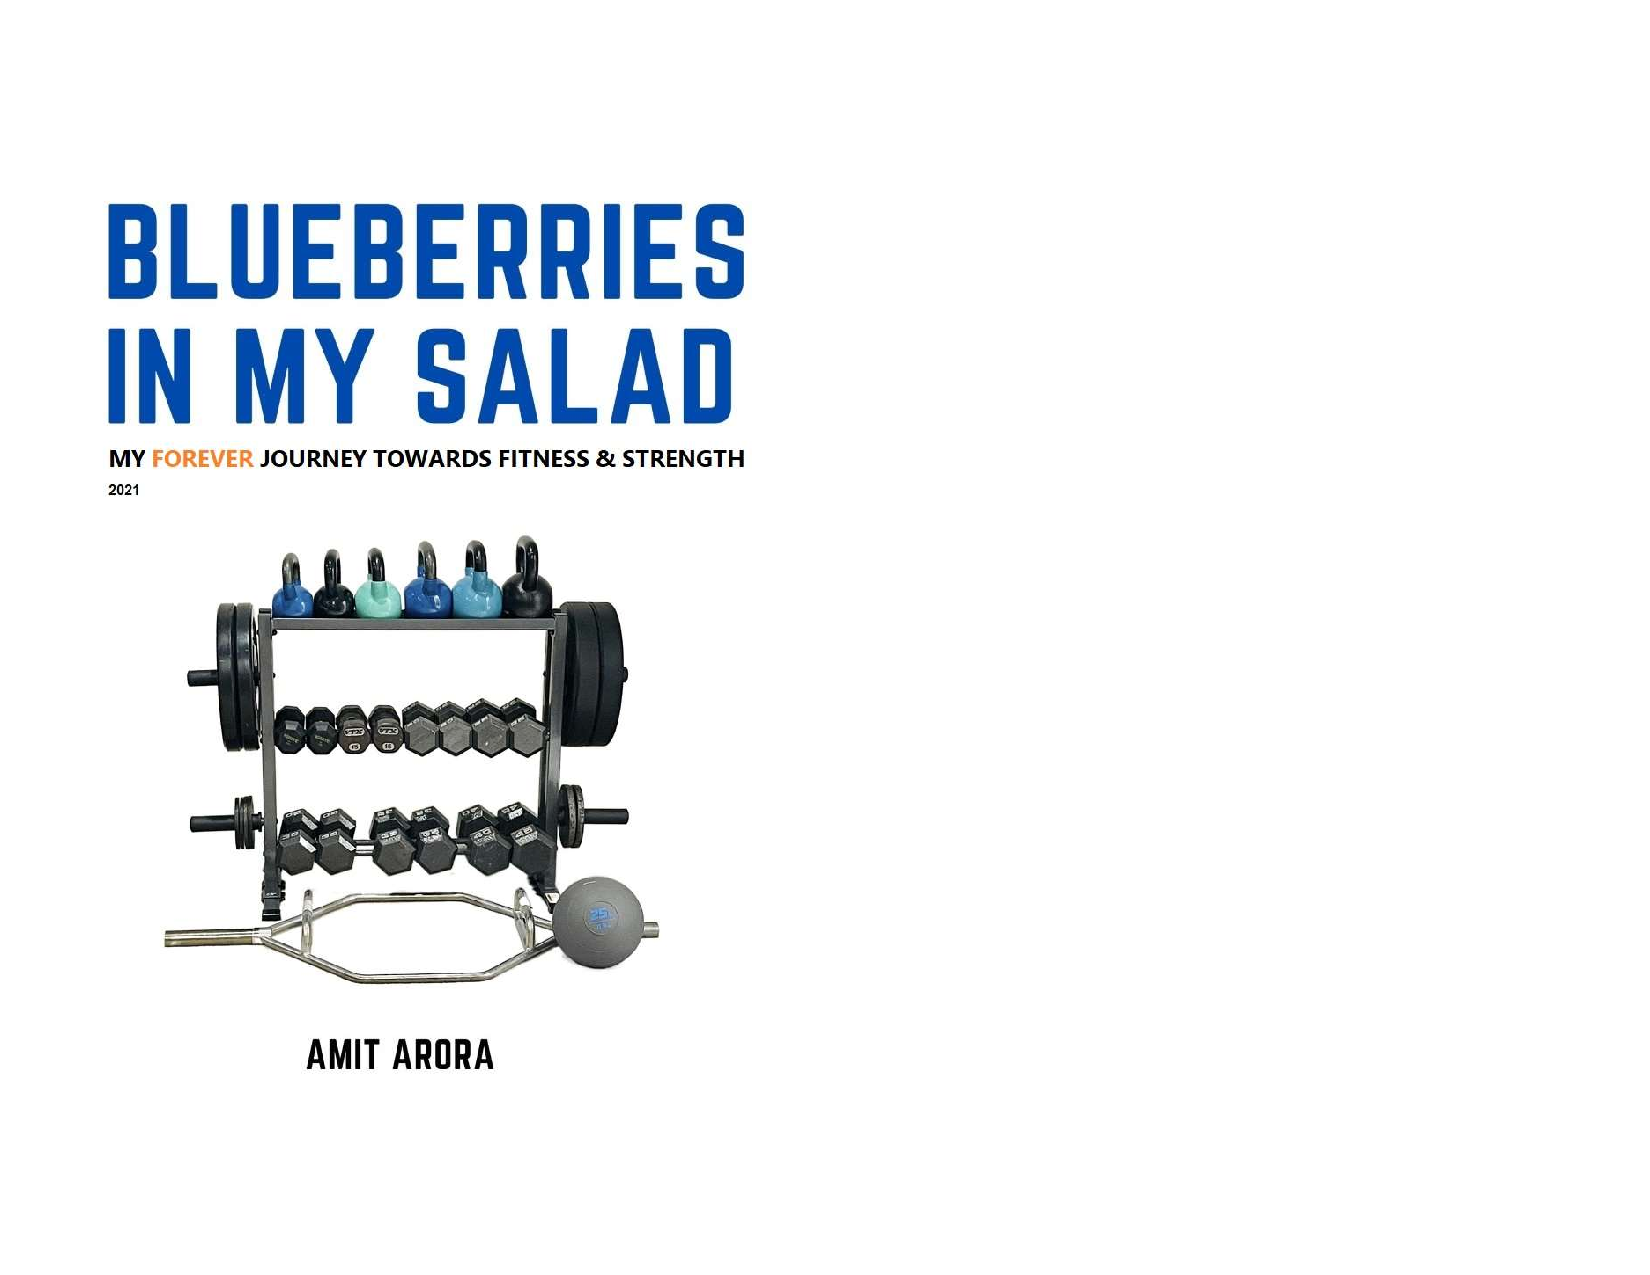
\includegraphics[width=\textwidth]{introduction/cover2021.pdf}}
\usepackage{amsmath}
\usepackage{booktabs}
\usepackage{caption}
\usepackage{longtable}
\ifLuaTeX
  \usepackage{selnolig}  % disable illegal ligatures
\fi

\begin{document}
\maketitle

{
\hypersetup{linkcolor=}
\setcounter{tocdepth}{1}
\tableofcontents
}
\setstretch{1.15}
\hypertarget{preface-to-the-updated-2nd-edition}{%
\chapter{Preface to the updated 2nd edition}\label{preface-to-the-updated-2nd-edition}}

I would not say that I wrote the first edition of this book (also, my first book) on a whim, but even so, it wasn't something that was a part of my new year's resolutions either. But then again, it was the year 2020 after all, between an online shopping site running out of podcast microphones and peacocks being sighted in city streets, anything was possible. A person like me who had been overweight and unfit most of their adult life suddenly writing a book on health and fitness, why not?

Since the 9 months or so that have elapsed between the first edition getting self-published and me starting work on the second edition, a few things happened. Firstly, I met several people, some close friends, some acquaintances and some complete strangers who told me how much they enjoyed reading the book, that it was useful for them in their own fitness journey and also they were curious if we eventually did reach our fitness goals (the first edition ends with me and my wife being about three quarters of the way there). I did reach my fitness goals both in terms of my body weight and deadlift target, so right there, there was a sequel to the first book waiting to be written. Secondly, I realized what a great learning and personal growth it was for me to actually put down all our experiences on paper and understand that it is one thing to hold your own in a conversation at a dinner party and a totally different thing to string together cogent and coherent sentences in a book. Finally, I learn and remember by writing (or typing). As they say one good habit begets another, I started reading and learning more and more, incorporating in my own life what I could about overall wellness, longevity, nutrition and other aspects of human health. I felt I should write what I learnt.

I am far from being an expert and certainly would not suggest to anyone to begin on this journey without proper guidance, but it is, after all, a voyage of self-discovery. This book is a travelogue of my midlife journey through the hills and valleys of health and fitness, discovering new (to me) vistas and realizing truths that now appear self-evident. Perhaps the most important truth that I learnt was that a choice between work and workout is a false binary. There is no work (as in a job, business, studies) without a workout. While it is mind over matter, always, but our physical body is also a tool to control the mind. A good workout does more for the mind than for the body, having experienced that repeatedly, I just cannot stress that enough. A good session of strength training is about as perfect a start to a day that you can ask for, it sets you up for success, give it a chance!

This edition of the book covers several new and important topics, such as ``breathwork'', ``water fasting'', ``proteins \& carbs'', and also a topic that has applicability even outside of fitness and strength: ``consistency rather than intensity, the power of showing up every day''.

When I started my journey, I was not sure of how long it would last. I never thought about it in terms of a start and a finish, I did not think much of anything except that this was a good road to travel. Most people I knew thought about health in terms of a single metric: \textbf{body weight}. People spoke in terms of ``oh, I need to lose 10 pounds'', ``I need to get rid of belly fat'' and so on, no one and I mean literally no one that I knew of spoke in terms of ``I want to have more energy'', ``I want to sleep better'', ``I want better physical fitness that helps me become better at whatever I do''. So when I started, my focus was also, not surprisingly, body weight, but over time I realized, body weight was just one metric, an important one, but still one of several. A healthy mind lives in a healthy body, and a healthy body takes consistent effort, day after day, week after week, month after month. Unless you have hit a genetic lottery and are just born with great metabolism there is a lot of work to put in (I would in fact argue that if you have hit the genetic lottery you have an obligation to maintain it). But a healthy lifestyle does not have to be a chore, people often get disappointed to hear that health is not a quick fix, the 10 pounds that they want to lose will come back once they go back to their old eating habits. \textbf{Lifelong changes require lifelong efforts}, and I would even question, why should it be any other way? There is a great amount of satisfaction and feeling of self-worth to be derived from looking back and reflecting ``Yes, I really did this, not as a onetime quick fix solution, but as something that I was able to sustain!''. What drives me is not just some goal that I decided to set up for myself but the experience, the blood, sweat and tears (metaphorically speaking) in the pursuit of the goal. Goals are important (a 400lb deadlift, completing the \href{https://themurphchallenge.com/}{murph challenge} in under 35 minutes, doing the \emph{Exorcist stairs} at Georgetown 10 times up and down, being able to run for 15 miles, many more) but those are more like milestones on a highway rather than a destination to get to. If I am making progress, howsoever small, even if it is two steps forward and one step backwards, it is all good. Fitness is an infinite game; the objective is to play the game for as long as possible and that can only happen by enjoying the journey and being proud of the effort.

For most of 2020 and early part of 2021, social interactions were severely curtailed because of Covid. As we started seeing people, it was interesting and encouraging to see that the reactions I got from people changed from ``how are you losing so much weight?'' to ``you look athletic!'' or ``you look strong!''. When someone praises you, it invariably creates a dopamine rush that drives you to keep up the good work. Whether it is an Instagram like or a compliment on your physical fitness, the physiological processes involved are the same, but I would argue getting the dopamine rush via someone saying nice things because you are a transformed person is probably not so bad! Just to be clear, I don't mind the Instagram likes at all. I put a lot of fitness content on my \href{https://www.instagram.com/ilivethedata/}{Instagram} primarily to chronicle my workout progress but also to maybe give hope to some random person (which would be me 2 years ago) scrolling through their Instagram feed and thinking ``if he can, then why can't I?''. It is always nice to see how far down that road I have traveled from being the clumsy person who could barely do a squat to someone who now regularly does a 150lb barbell squat.

A word about data, we kept up with the practice of collecting weight and other biometrics every day and that has been invaluable. I would have liked to have better tracking for all exercises but did not find an app which did quite what I wanted. Started creating my own app for tracking workouts, but with my day job, I could either find time to work on the app or write this book, I choose this book :). Hopefully, the app will also be available someday. The charts and tables in this book are all generated using R and gpplot2, please see this \href{https://github.com/aarora79/biomettracker}{github repo} to find the latest data. This book is rendered using the wonderful \href{https://bookdown.org/}{bookdown package}, very thankful for it.

As all good books should, this book too has a website now. Please see \url{https://blueberriesinmysalad.com}. The website tracks our journey as it continues, has updates on what are the latest topics in health and fitness that I am currently learning about and maybe a monthly newsletter as well in the future.

Amit Arora\\
Clarksburg, Maryland

PS: To the one person who sent me screenshots of underlined passages of the first edition of this book with questions written on the margin, thank you for the encouragement :), please look for a signed hardcover copy of this new edition in the mail!

\hypertarget{preface-to-the-1st-edition}{%
\chapter{Preface to the 1st edition}\label{preface-to-the-1st-edition}}

This is neither a book on salads, nor a commentary on life. What it is, is a journal of experiences that my wife and me had in our journey towards being fit and strong. Like a salad, day to day life may not be the most appealing lunch option, but just like a good salad if you can keep finding the blueberries every now and again, it is both rewarding and fulfilling. The small and big milestones we achieved during our journey kept us going, just like the blueberries in our salad.

Initially, I wanted to write a book documenting our journey towards fitness and strength on a day to day or at least a week by week basis. As things progressed, I realized that we were not the only ones on this journey and the Internet was filled with blogs and YouTube videos that document in detail, very successful, inspiring and transformational stories. Why was I wanting to reinvent the wheel by writing our story on the same lines? I thought that while a daily or weekly journal was not something, I could do but definitely there were ``topics'' on which I would like to pen down my thoughts. For example, the most often asked question, ``What diet did we follow?'', ``Do I really need a trainer?'', ``Just tell me how long it would take to lose 10 pounds'' and so on. Therefore, I decided to write this book as a collection of essays on these and other related topics.

It has been more than 9 months since we started this journey and I feel that we have learnt so much that it is important to document this first and foremost for our own selves and then also for anyone who might be interested (I hope someone is). After all, it is one thing to see someone famous transform and another thing to see someone you know or could relate to (middle aged Punjabi NRI couple anyone?) do the same and then realize ``If they could do it, so can I''.

We took daily measurements for our weight and other biometrics and they were automatically synced via an app on our phone. This is huge, daily tracking enables, even forces, conversations around progress (or lack thereof) towards your targets. It keeps you honest and on track. What it also enables is to see the big picture over time, such as are you slowing down, do you need to adjust to your routine, how much that elaborate weekend dinner set you back? For me personally, as a data scientist it was fascinating to collect the raw data, find patterns, gain insights and get some forecasts done (when would we reach our target weight?).

Over time I understood that while the desire for weight loss was what got me here, but what I was really gaining was good health and strength. One can lose weight by falling sick, we know that is not healthy. Weight loss should not be the only goal. To reduce the benefits of what we were doing to just burning calories and losing tens of pounds now seems like a terrible underselling of the idea of fitness. The human body is a fascinating machine capable of wonderful things, good health is a state of both mind and body. Exercise and healthy eating habits help both mind and body. If you do not have any serious health issues, there isn't really any excuse for not exercising regularly and eating healthy. As it is said 
\includegraphics{pictures/sanskrit1.png} loosely translated it means that the body is the source of all good deeds.

Finally, nothing in this book should be interpreted as me recommending anything, this is simply a written version of my musings. An experiment with a sample size of N=2, in other words statistically irrelevant! \textbf{Do not take anything that you read in this book as medical advice. Always consult your doctor before starting any diet or exercise program.}

\hypertarget{acknowledgements}{%
\section{Acknowledgements}\label{acknowledgements}}

Besides improving our quality of life, clean eating and exercises also provided me the impetus to finally take up something that I have wanted to do for a long time, writing a book.

This would not have been possible without my dear wife Nidhi, who was not only an equal partner in this journey but was also the head chef to prepare all the tasty \& nutritious food (all the photographs including the book cover are courtesy her), the assistant coach who kept an eagle eye on my forms during the exercise and also the one who kept on encouraging me to write. She is also the proofreader for this book, although, any mistakes and omissions are mine alone.

A huge thank you is due to our wonderful trainer and friend, Dawn Kirk. Thank you Dawn for persisting and persevering with us. I wish everyone has the good fortune to have a trainer like you.

Finally, this book is dedicated to my grandparents, my guardian angels. I know they watch over me.

Amit Arora\\
Clarksburg, Maryland

\hypertarget{how-it-began}{%
\chapter{How it began\ldots{}}\label{how-it-began}}

I remember the first time some 15 years ago when a colleague at work introduced me to the burrito, and delicious as it was, I barely managed to finish it. Same with the foot-long. It was just too much food, more than what I needed to eat for lunch. Over the years I got more used to it and what used to be a huge portion size once, was just very normal now. What was almost a culture shock many years ago, was just routine now. It should not have been.

About 3 years ago i.e.~in the spring of 2017, I decided to go to the doctor and ask why do I wake up with a severe case of dry mouth every morning? I knew I was grossly over-weight and the dry mouth had started happening a few years ago and the two could be related. I kept ignoring it for years, but it had become bad enough that I sometimes used to wake up very early in the morning because of it and had to rinse my mouth to go back to sleep. The doctor's visit was an eye opener, he said it is most certainly because you are grossly over-weight (I weighed 273 pounds) but asked a few more questions which led him to believe I had all the symptoms of sleep apnea.

TL;DR I did a home sleep apnea test and the results were very alarming. The doctor said it was so bad that I could be at the stage of starting to lose short term memory i.e.~because the sleep is so disrupted because of lack of oxygen that the brain is not able to make new neural connections that it usually does when we are sleeping. This was happening when I had just joined a masters program in data science at Georgetown University and was now part time at school, 16 years after having completed my engineering degree. With my day job and school homework, my sleep time was anyway much reduced and not getting quality sleep was just bad in so many ways.

\hypertarget{my-tryst-with-a-protein-based-diet}{%
\section{My tryst with a protein-based diet}\label{my-tryst-with-a-protein-based-diet}}

Something had to be done. I got on a medically supervised weight loss program that used a ketogenic/protein meal replacement diet and I started sleeping with a CPAP (Continuous positive airway pressure therapy). I count those two decisions among the top 5 best decisions of all time I ever took in my life. I followed the diet very strictly, of course my dear wife Nidhi was with me in this and she did the diet as well. I started losing weight immediately, sleeping with the CPAP machine was what I would call a life changing experience. I no longer felt like dozing off while driving to college, even if I slept 5 hours (which was 4 days a week) I still woke up refreshed and did not experience the mid afternoon crash in energy. In a couple of months, the weight loss, for both me and my wife, was very noticeable and friends and family started asking what were we doing that was causing this transformation. Everyone is interested in the new diet that their friends are into (especially if they are getting thinner:)). Expected case of FOMO, I would say. In about 8 to 9 months, I had lost close to 70 pounds and my wife had lost close to 40 pounds, that is drastic by any measure. It was effective, expensive and un-sustainable!

For about 10 months or so till I followed the diet, we were pretty strict about no or as little carbohydrates as possible and ate a lot of those protein supplements (bars, shakes, snacks etc.). Then came the holiday season, new year parties and there it was, the dreaded phase where I thought OK, we can go off course for a little bit and then get back on when this season is over. No prizes for guessing, it never happened. I still remember my weight had gone down to 202 pounds and I could see it rising back up, day after day. I thought OK, this is still less than 210, I can pull it back, no problem. Well, not really, soon it was past 210. I told myself, OK but it is not 220 yet, I can pull this back. Once it crossed the 230 pounds mark, I gave up trying.

I was able to graduate two years later (in 2019), my weight at 240 pounds and the CPAP machine by my bed every night. I did not even go for a weekend getaway without it. The dry mouth was getting back, not as bad though, but it was back, there was no missing it. The sleep was not as good. By end of 2019, I was 250 pounds, the CPAP machine was broken, my wardrobe almost completely redone because none of the clothes fit me anymore and I had given away all the clothes from 2017.

\hypertarget{a-new-beginning}{%
\section{A new beginning}\label{a-new-beginning}}

Cliched as it is, I made a new year resolution in Jan 2020, ``I need to fix myself, this cannot continue''. Nidhi had also gained weight, not as much as me, but she gained 20 pounds out of the 40 she had lost. She had mentioned to me in December 2019 that there was this personal trainer who had dropped in to the Doctor's office (I conveniently skipped to mention that Nidhi became a health coach and started volunteering in the Doctor's office) and left her card if someone coming in for fitness training wanted to come for a trial class at her gym.

It is said, good things happen when the time is right (no one says that, I just made that one up :)). Nidhi left the trainer a message, and we did not hear back from her until a few days later when she said sure we could stop by her gym for a free class. There we were, on January 17th, 2020, in her gym, for what I did not know at the time would be the start of a new chapter in our life.

The gym itself was unassuming, in an extended but disjoint part of her house. I did not think much of it, but little did I know what we were getting into. It needs to be said that prior to this I had never seen the inside of a gym in real life and my only window into how fitness equipment looks like and what trainers do was through films and TV, in other words, what I knew was far from reality. I remember asking before the training ``So what do you think, how many calories would we burn during the workout today?'' and the answer I got was ``Oh I don't know, we don't count calories here :)''. ``Ok, then'' I remember saying to myself. The trainer seemed to be a pleasant person with an infectious smile, the training was good, tiring but not hard and I was like ``OK, this isn't too bad''. Later that evening, I felt a sharp pain in my neck, but I thought it is nothing. As the evening progressed, the pain increased. I barely got any sleep that night, even after putting some pain reliving ointments, the pain did not subside. It was the most physical pain I had endured in a long time. I even thought to myself, maybe I would need to put in a collar around my neck (I didn't need to). It took a couple of days for the pain to go away completely. Thankfully, that was the only time I felt such pain in all the months now that we have been exercising. Was a good lesson for me right at the start, never be under any false sense of bravado while working out in the gym (or even otherwise :)).

We decided to enroll for two classes a week. Since we were just starting out and I needed individual attention, we decided why don't we do a couple's package where we would have classes for a month for just the two of us together. She also asked us to fill out a detailed log, as detailed as we could get, of everything we ate or drank for 3 consecutive days. It was not convenient, but we scribbled something and gave it to her in the next class. The trainer had a small book that she and her husband had written about her journey with what they called (don't know it might be a standard term) ``clean eating''. There is a 30-day clean eating challenge in which you eat no processed food, no dairy, no pulses, no legumes, no hard drinks and no soft drinks either, only vegetables, fruits and meats are allowed. We decided to do the challenge and made a list of everything we thought we could eat during the challenge and got her to say Yay or Nay on each of those items. The list is in appendix A of this book. It had things commonly found in Indian kitchens like ``spices'', ``herbs'', different fruits etc. Now that I think about it, I am not sure what made me do the challenge, I just decided to do it just like I decided to workout in the gym twice a week, something that I had never done in almost my 41 years of life. When thoughts become deep, intentions become weak. So, there we were, working out twice a week in the gym and decided to go for clean eating in a few weeks' time.

What endeared me to the workout sessions was that after a few weeks I noticed both in myself and my wife there was an unmistakable feeling of joy/elation/happiness as we completed a hard training session in the gym. We did lose some pounds but nothing very noticeable. What attracted me to the clean eating was that I could identify with it, it did not claim any magic results, did not ask to give up on the basics i.e.~vegetables/fruits/meat in fact it embraced these and only said do not eat processed food. This was the same guidance I had grown up with during my childhood, this was what my grandmother used to say as well, surely this could not go wrong. Surely nothing bad could happen by not eating cakes and cookies, not drinking soft drinks or hard drinks and just basically saying goodbye to processed sugar. Made total sense.

So here we were, ready to start and reminding ourselves \textbf{that the only way to reach the finish line is to start\ldots{}}. My target was simple i.e.~``not to be obese'' as per the \href{https://www.nhlbi.nih.gov/health/educational/healthdisp/pdf/tipsheets/Are-You-at-a-Healthy-Weight.pdf}{NIH guidelines}, provided. I do not remember the time I was at 158 pounds, I just wanted to be 190 or less so that I would not be adding to the ``obese'' population of the planet. Nidhi on the other hand was reasonably fit and her goal was close to the NIH guidelines. I had the motivation, the means and had made up my mind.

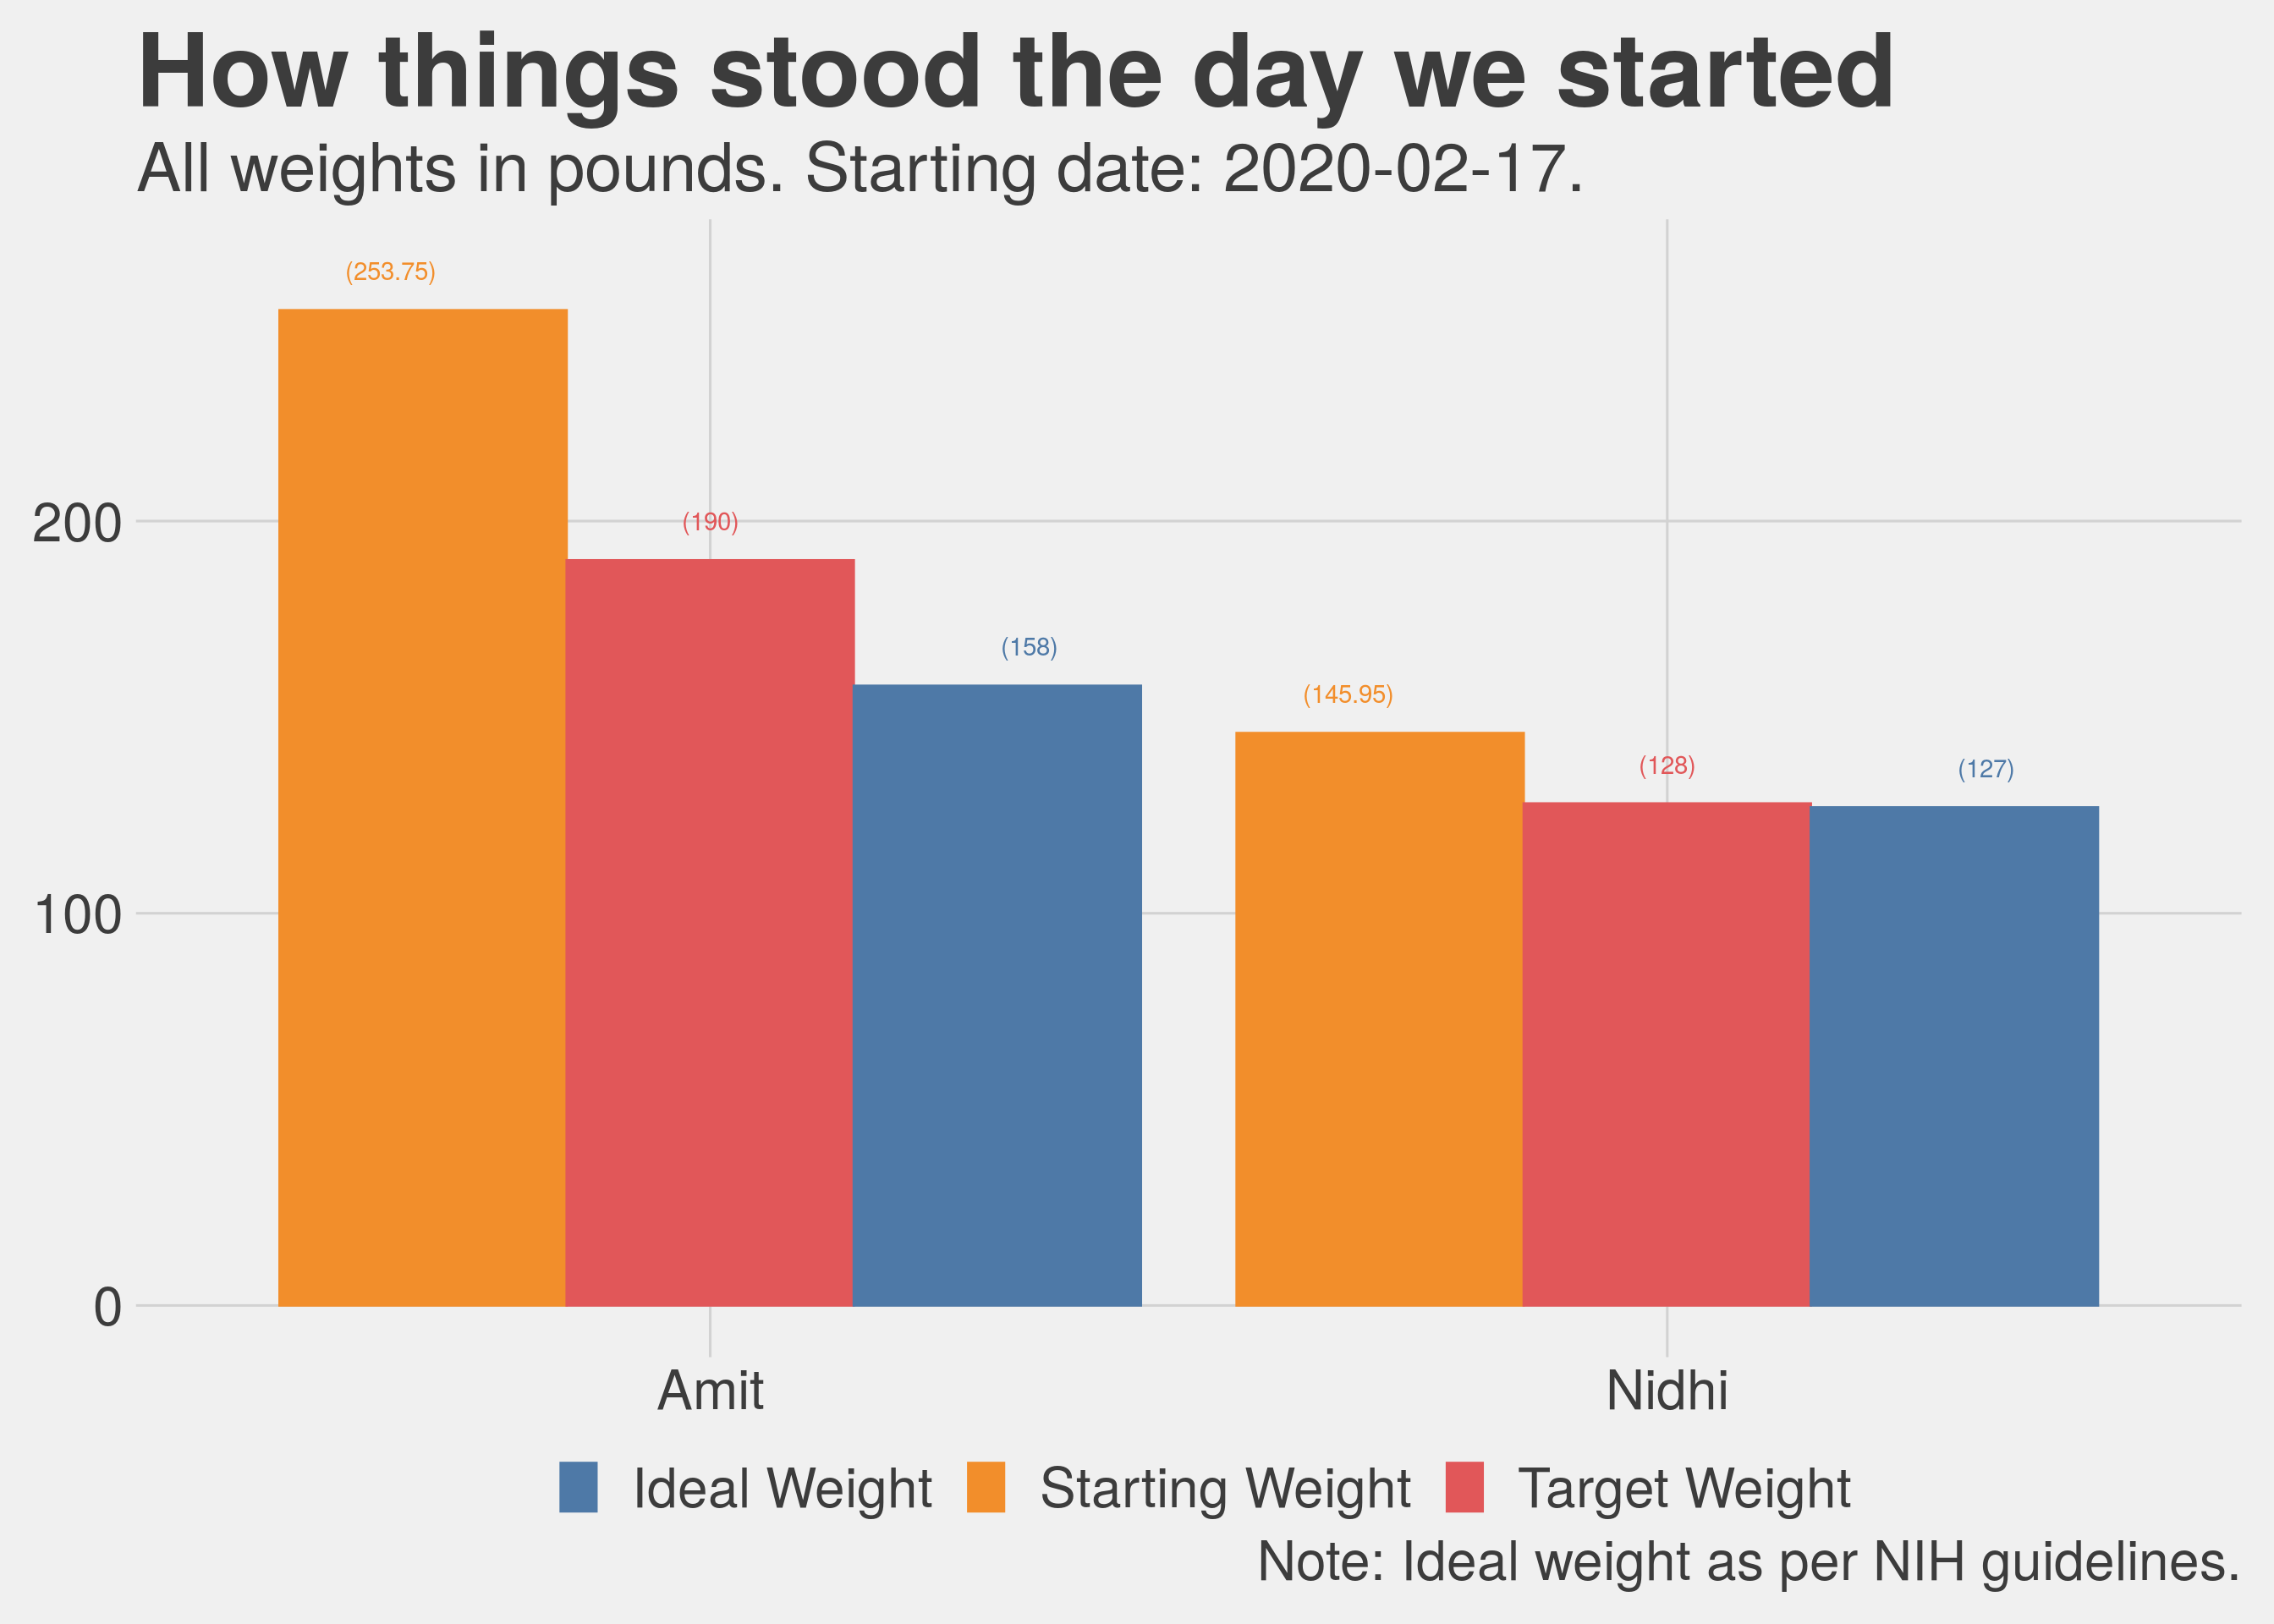
\includegraphics{bookdownproj_files/figure-latex/unnamed-chunk-4-1.pdf}

\hypertarget{looking-back}{%
\section{Looking back}\label{looking-back}}

With the benefit of hindsight having been on this journey for close to two years now, here are some closing thoughts for this chapter on new beginnings.

Whenever we start something new, even if it is something as personal and discrete as a change in eating habits and fitness regimen, as people around us learn about it there are two kind of reactions one can expect, broadly speaking. One is a reaction of genuine encouragement which comes from a place of care, concern and wellbeing. This is usually from immediate family and close friends. The second is that of nonchalance disguised as an overt display of encouragement. Almost as if to say that you are trying a new fad, sure, try it for a few weeks, soon you would give up and be back to the same place as all of us or as a data scientist would call it, ``you would regress to the mean''. We should use both these reactions in a positive manner, even people who are indifferent today would be appreciative when they see the results in the months and years that follow (I purposefully did not say ``weeks'' but months and years). The fact that we started our journey in 2020 did help in this regard, we hardly met anyone in person for a greater part of the year, so most of the external inputs at the start of our journey, were just not present so we did not have to deal with them. While some of us might be completely self-driven with no need for the fuel of external encouragement to power our journey, but most aren't. As I realized later, it feels good to be appreciated :). Nothing like a little bit of positive reinforcement from family, friends, acquaintances or a random person walking up to you in a social gathering to say ``you look so much fitter than last I saw you, what have you been doing?'' to fire those dopamine neurons which will make you get up and move (very literally).

I would end this chapter by saying most people overestimate what they can achieve in the short term and underestimate what they can achieve in the long-term. Usually what we think of as short term targets either don't get achieved because they were never achievable in the short term to begin with (like fitness, wealth creation) or even if they are achieved we end up losing them (again, fitness and wealth creation seem to be the perfect examples here). In the world we live in today, setting your eyes on a long term goal and then working towards it without getting discouraged by failures that would inevitably happen along the way is a little bit of a challenge. If someone told me in January of 2020 that it would take 15 months of a lifestyle change comprising of nutrition and regular workouts to reach to my weight and BMI goals, I would have had moments of self-doubt. The trick is to acknowledge the self-doubts but focus on the resolve or maybe just don't think anything at all and just take the plunge (which is what I did). You would be surprised to see encouragement pouring in from unexpected quarters, the universe does conspire to make you successful!

\hypertarget{chapter-3-at-a-glance}{%
\section{Chapter 3: At a glance}\label{chapter-3-at-a-glance}}

\begin{center}\rule{0.5\linewidth}{0.5pt}\end{center}

\begin{enumerate}
\def\labelenumi{\arabic{enumi}.}
\item
  A change in lifestyle is usually triggered by a life changing event which often is a health scare. Don't wait for it to happen, make the switch to a sustainable healthy lifestyle now.
\item
  If the change you make is not something you can sustain for a long time, it will not last and ultimately all the gains you made would be lost. We found that a high protein low carb diet and no workouts, did not work for us as we found it to be unsustainable.
\item
  Clean eating and with regular workouts could be an ideal start for someone trying to make the switch.
\end{enumerate}

\hypertarget{clean-eating}{%
\chapter{Clean Eating}\label{clean-eating}}

\emph{Disclaimer: this is my interpretation of what I understood and did as part of clean eating. I am not aware if there is a standard definition for this and if there is one I do not wish to challenge it.}

Clean eating is not a diet. This is the number one thing I find myself explaining to people when they say, ``you have lost so much, what diet are you following''. It is simply a decision of saying I am going to keep processed foods and sugars out of my body. Strictly speaking, only if you are eating something you have grown or you have hunted are you eating clean, but then let's be real here, unless you are living on a farm, this is not feasible. The next best thing we could do is to keep processed food and especially processed sugars out of our body. I don't need to say more on this except that there is tons of research available proving why processed food and refined sugars are just plain bad, do yourself a favor stay away from these.

Appendix A contains a checklist of what we confirmed with our trainer was allowed during clean eating. This is an exhaustive list. Before I get into the details of exactly what we ate, I would like to address something upfront. Is clean eating hard? Yes, it is hard, but only to the extent of saying that nothing that is worthwhile is ever easy. Not being able to eat your favorite unhealthy snack is hard, I am not going to lie, but then it is for a fixed period. After all, no one ever became unhealthy because they could not eat enough ice-creams :). At the same time, clean eating is also not that hard when I compare it to other diets. The key difference is that you are not counting calories, counting calories is not sustainable, you cannot survive on 1000 calories a day for long (several months maybe, can you do it for your whole life). Think of it, if counting calories was the solution then some food company would have figured it out and the shelves would be full of some magic food.

The intent of clean eating is to reset your system, calibrate your taste buds so that they begin to appreciate the natural tastes of different foods. I would know because I am the person who back in India would go (every now and then) for a late evening after dinner ice-cream (a fruit salad Sunday to be precise) and then as if that was not sweet enough, go to a \href{https://en.wikipedia.org/wiki/Kulfi}{Kulfi} place right after that to top it off! 3 weeks into clean eating I found a papaya to be sweet, grapes to be just too sweet and eating an orange or two as a 4pm snack seemed just delightful.

Indulge me a little bit before we get into the details of breakfast/lunch/dinner. When we got married, we went to Europe for our honeymoon and one of the places we visited was the city of Nice in the south of France. Absolutely beautiful place, however, we did not quite develop an appreciation for the French food. We were looking for some Indian food or anything that had some spices and was not cold and bland (my apologies to anyone reading and thinking these folks don't know the first thing about French food). We found this Pakistani restaurant by the beach and were delighted to eat some Butter Chicken there. It was not hard to notice that we were from India because Nidhi was still wearing some distinctly Indian jewelry. The owner of the restaurant stopped by to talk to us and seeing we were Indian sat down for a conversation. He said, ``you know, the French food is the best food in the world'', we were listening but not quite agreeing, the butter chicken would not allow us. He continued ``back home, we put so much spices in our food, cook it for so long that we never get to know what the ingredients actually tasted like\ldots{}''. Months of eating relatively clean (not strictly, I mean I do eat my ice-cream sometimes, I have had a pizza a few times), has made me realize that while I still cannot compare the taste of the Indian cooking with anything else, I do see the point of the natural taste of food. Our elder son likes a green chilly with his dinner, but the younger refuses to even recognize that ``bitter'' can also be a taste.

\hypertarget{a-clean-breakfast}{%
\section{A clean breakfast}\label{a-clean-breakfast}}

Breakfast was mostly eggs, in any form. Egg fry (cooked in Ghee or Kerrygold butter), Omelette (sometimes with tiny pieces of bacon thrown in), boiled eggs, scrambled eggs, egg wrap or any other variation one can think of. Along with coffee (for me, I am a coffee person) or tea (Nidhi is a tea person) with almond milk or an almond and coconut milk creamer. We used to think that removing dairy from our diet would be almost impossible, but surprisingly, that was one of the easiest things to do. Swapping whole milk with almond milk worked like a charm. I personally find the almond milk so light and have developed such a liking for it that I no longer feel like drinking regular milk at all. For the days we did not consume eggs, we had bananas or almond flour pan cakes. Another thing we really enjoyed for breakfast was frozen Acai bowl (you can get them at Costco, just don't eat the granola that comes along with it).

Here are some pictures. I would note that every day the Omelette may not have looked as good but was close. It is real hard work to make breakfast this good daily and the credit for this is one person's and one person's alone i.e.~Nidhi :).

\begin{figure}
\centering
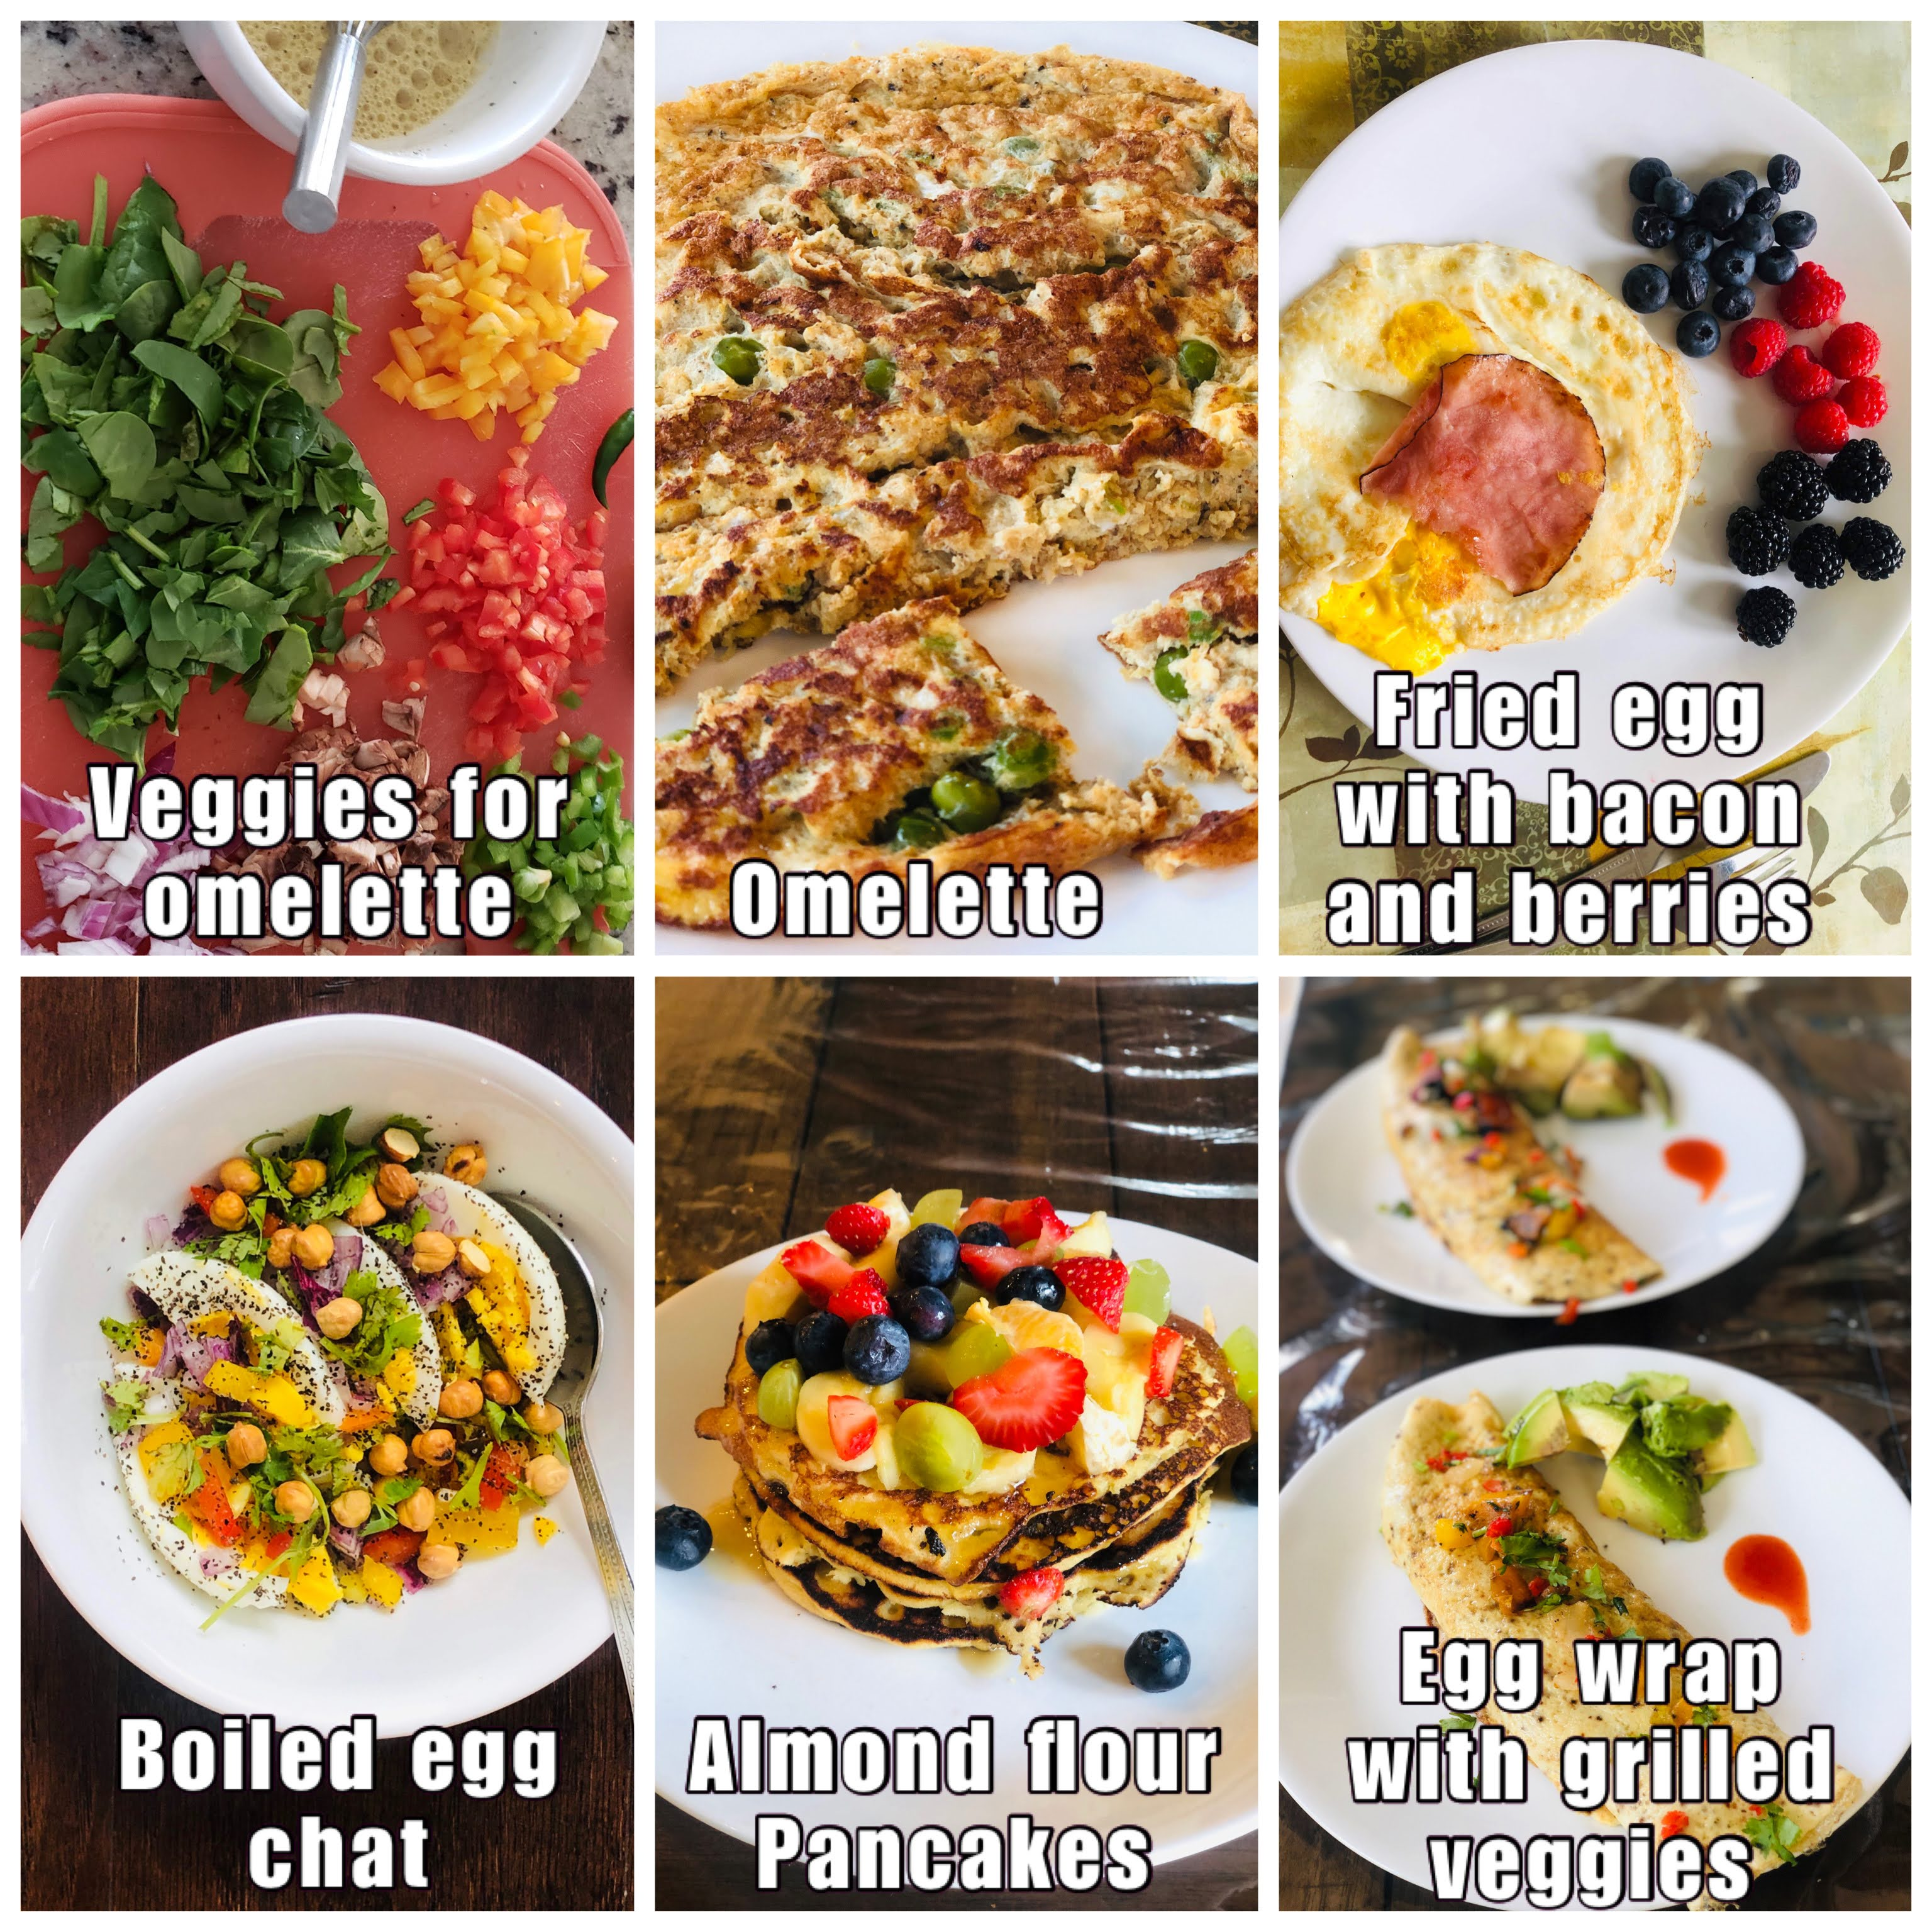
\includegraphics{pictures/breakfast.JPG}
\caption{A clean breakfast}
\end{figure}

\pagebreak

\hypertarget{a-lunch-we-really-love}{%
\section{A lunch we really love}\label{a-lunch-we-really-love}}

For lunch we used to have salads. I don't know about you but when I think of salads, i have two contrasting pictures in my head as reference (this is all prior to clean eating), one is a cold salad with raw vegetables and boiled eggs, along with some beans and chickpeas and broccoli and the other image is from a salad place like the one I often visited at Georgetown, exquisite salads with all sorts of ``woke'' ingredients. The first one was something I just did not find palatable at all and the second one was what I would wait for the whole week so that I could eat it whenever I was at Georgetown for a class. Surely there was some middle ground here, I would think, and there is.

Costco has a bunch of good salad mixtures in their fridge section and they are all very good. We particularly liked the sweet kale salad (minus the dressing that comes with it, we did not use that). So we mixed the sweet kale, with additional ingredients such as spinach or other mixed greens and topped it with sunflower seeds, chia seeds, walnuts (sometimes cashews), some cranberries and my favorite, ``blueberries''. Used a homemade dressing made of olive oil, lemon juice and herbs. Add a boiled egg, half an avocado and then either some grilled chicken or tuna. Some days we substituted chicken/tuna with grilled tofu. I am still surprised that even after more than 6 months of eating variants of it (keeping the base recipe the same) 4 to 5 times a week, we are still not bored of it, in fact we seem to like it as much as we liked it before. Each day, the salad tastes a little different and that was keeps it interesting.

\begin{figure}
\centering
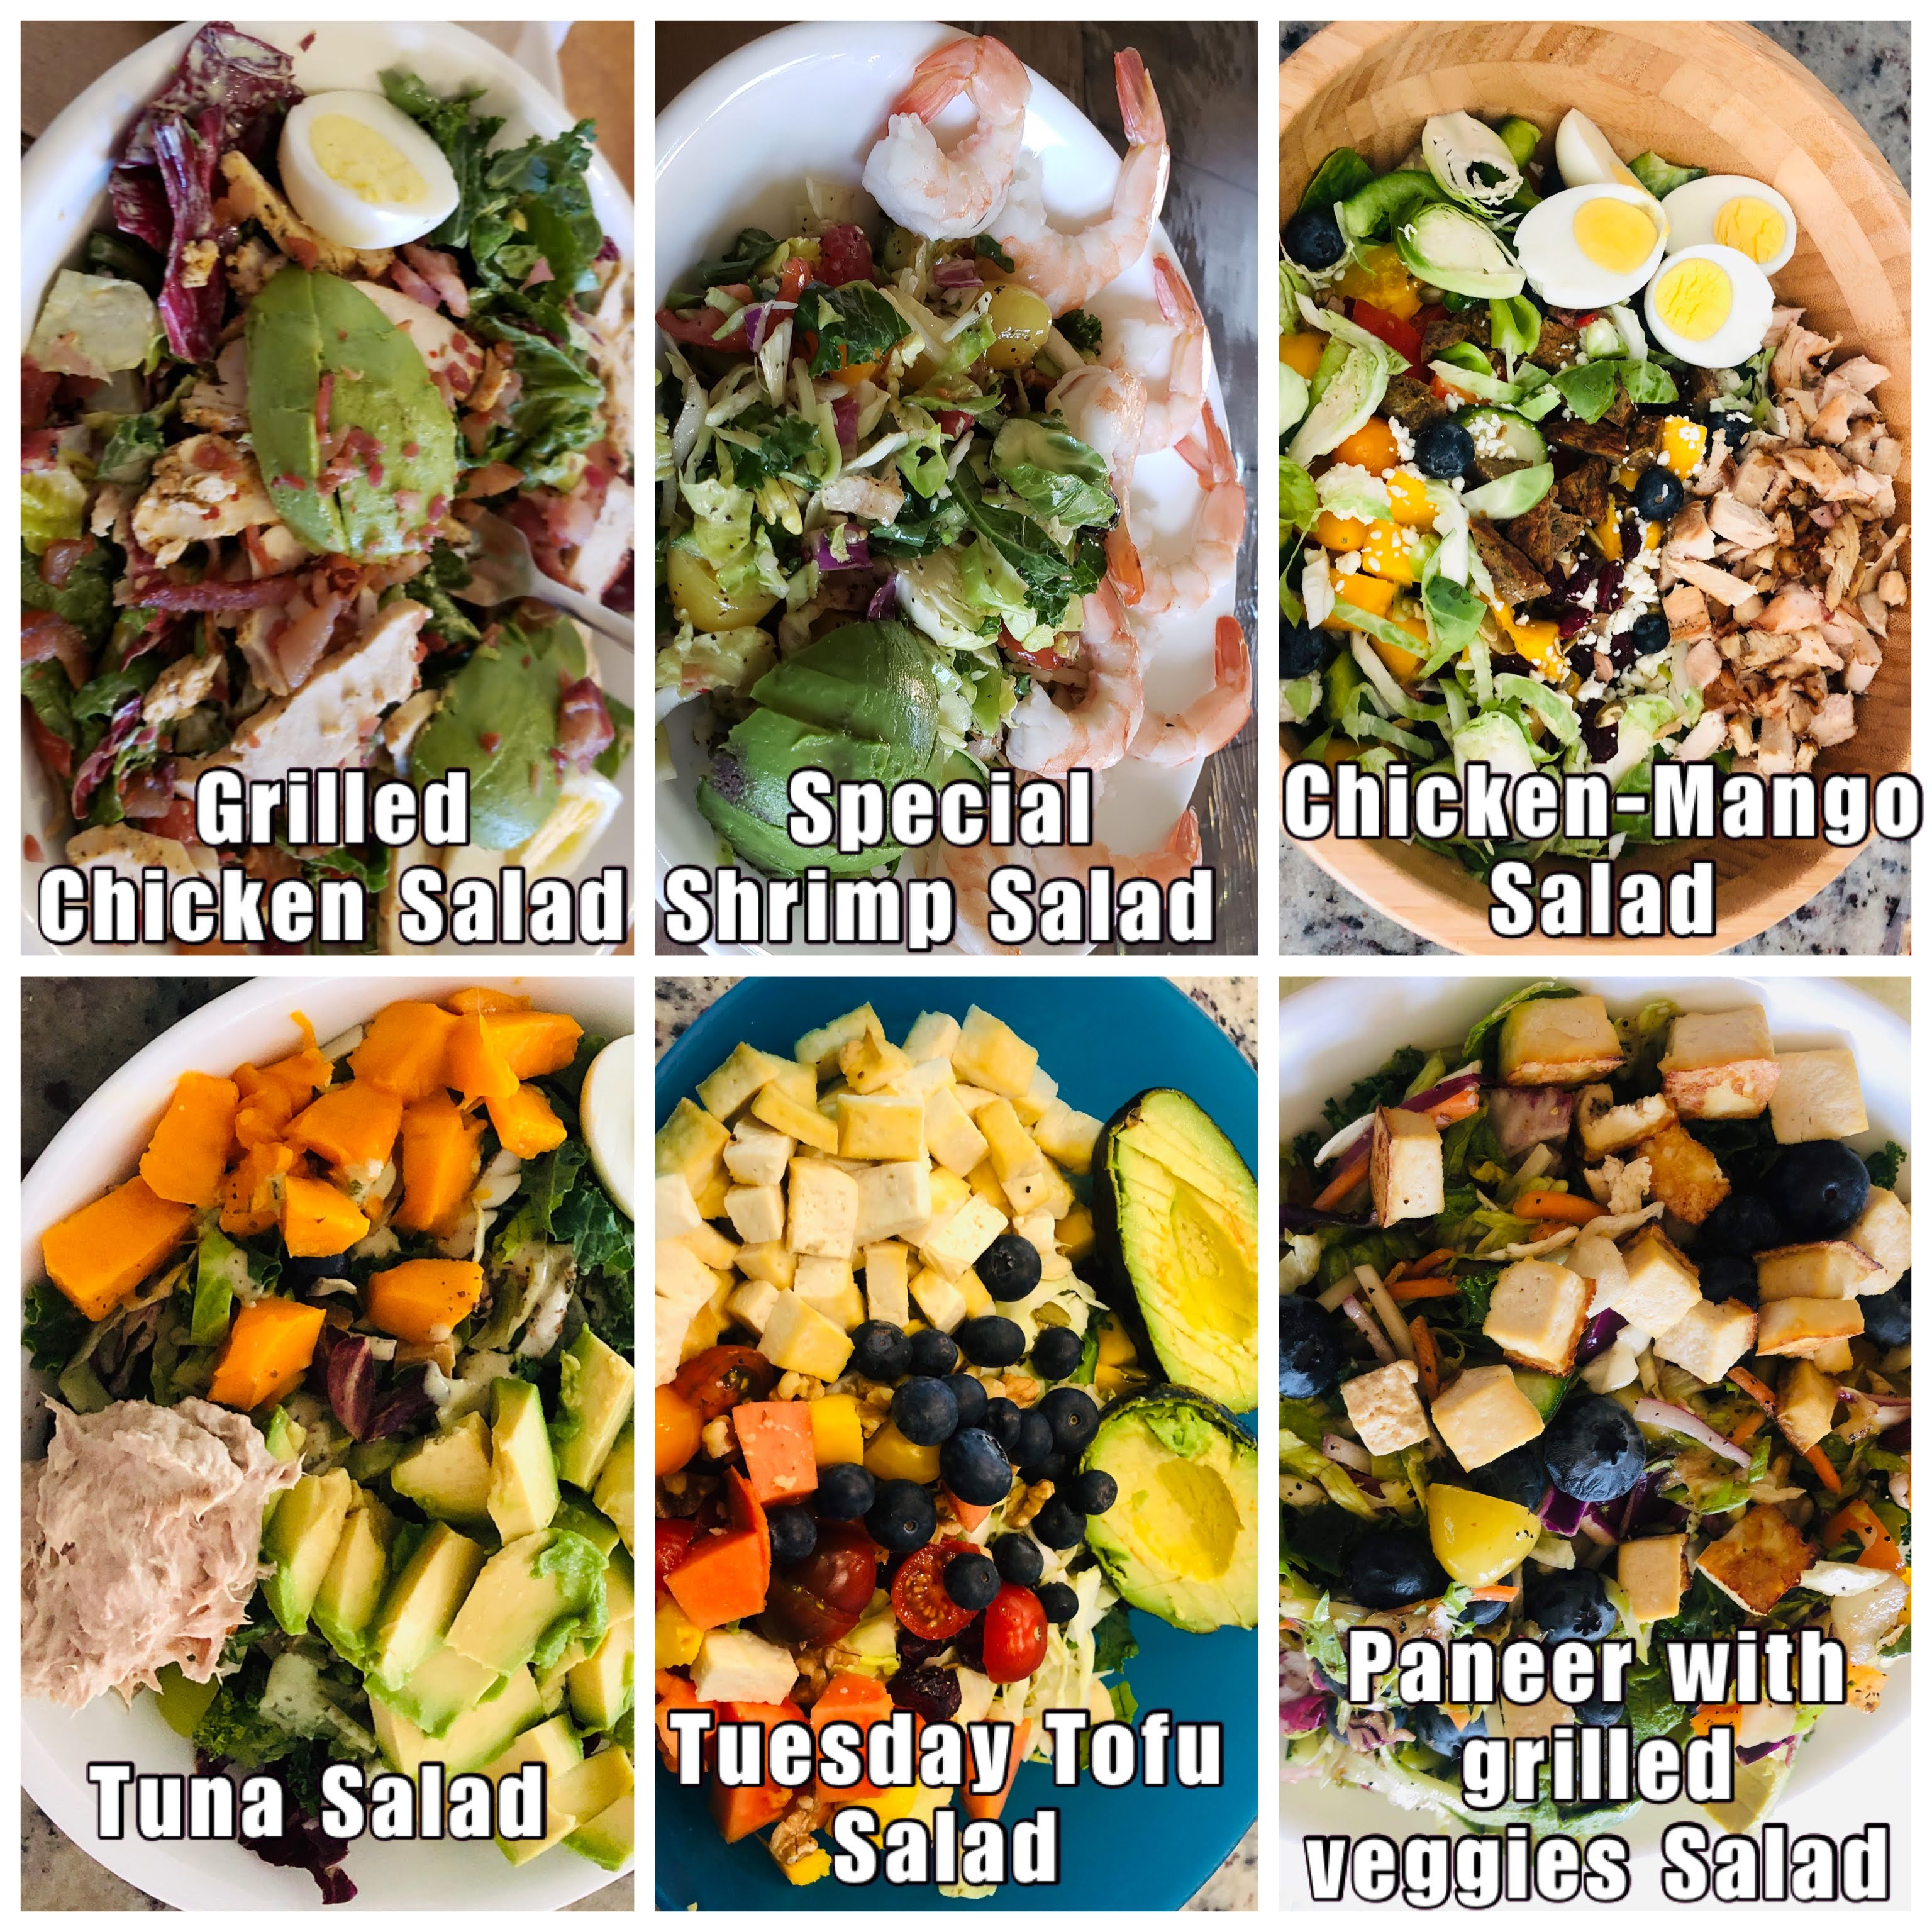
\includegraphics{pictures/lunch-salads.JPG}
\caption{The lunch salad collection}
\end{figure}

One of thoughts I had, and I believe many people would have is that salad does not satiate me, it does not fill me up. That was not the case for us as I found out. Eating a bowl and a half of salad does indeed fill you up. As before, I still like a cup of hot coffee after lunch. What does happen is that after 2 to 3 hours I felt the need for a late afternoon snack. Previously this could have been any unhealthy options like chips, cookies, a diet soda, even a chocolate bar, basically anything you would typically find in a vending machine. That had to go, for good.

\hypertarget{the-4pm-snack}{%
\section{The 4pm snack}\label{the-4pm-snack}}

A couple of small oranges at 4pm felt delightful. They tasted good, and the sugar content provides the boost the brain needs to shake off any late afternoon lethargy or drowsiness. At times I also ate maybe 4 to 5 apricots, maybe an apple, or even some nuts such as walnuts/cashew nuts/almonds (not those packaged snack pouches please, we want to stay away from any processed food, as much as possible).

I did not try this as much, but sometimes I did have a ``tea'' such as a earl gray or English Breakfast, just a dip tea with hot water, no milk of any kind. It was nice, but me not being a tea person did not pursue it that much, but it is certainly an option.

\begin{figure}
\centering
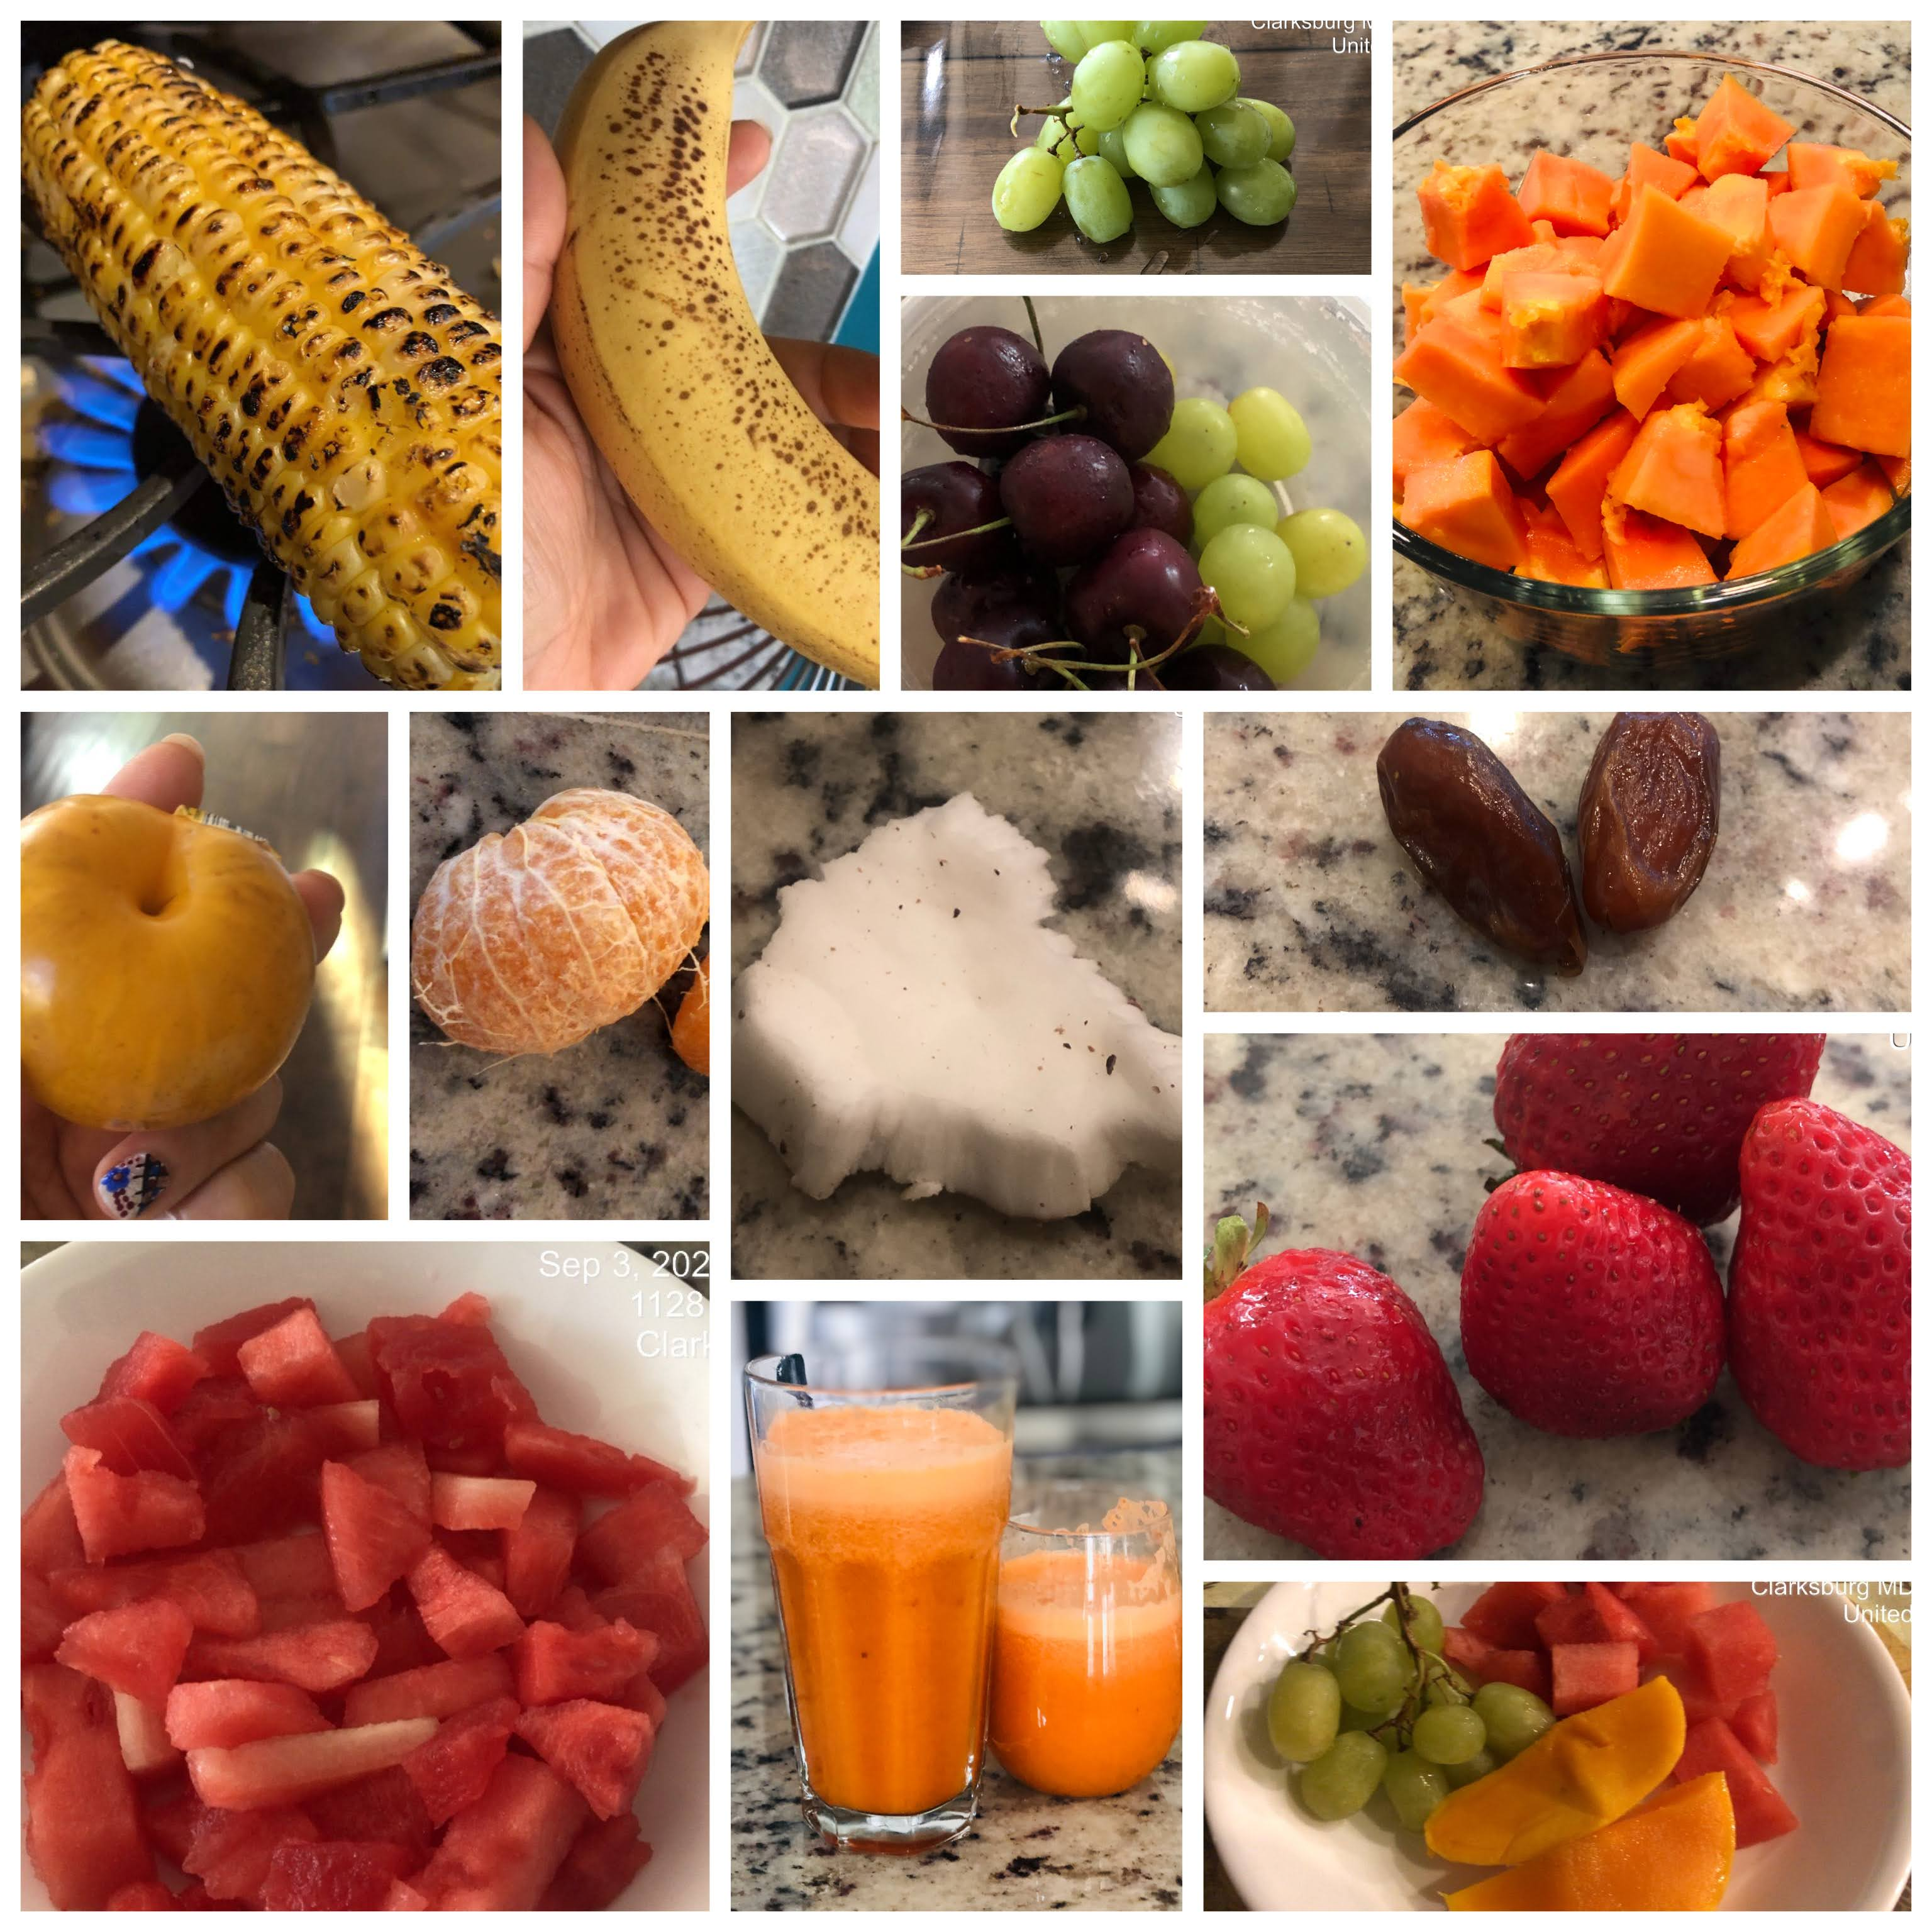
\includegraphics{pictures/4pm-snacks.JPG}
\caption{The 4pm snacks}
\end{figure}

\pagebreak

\hypertarget{the-grand-finale-a.k.a-the-dinner}{%
\section{The grand finale a.k.a the dinner}\label{the-grand-finale-a.k.a-the-dinner}}

If you try to stick to this routine, you would naturally find that you want to have your dinner early. What is early? For me, growing up, dinner was never earlier than 7.30pm and then later in life as I got caught up with studies and then later at work and other things, it could be at 8 or 9pm or even later. That is not good, in fact, I would now say that is just unacceptable.

Now we really try to wrap up dinner by 7.30pm, maybe 8pm at the latest. I start feeling hungry around 6pm, so a dinner around 7pm seems like the perfect fit. Eating dinner early helps to naturally avoid the urge for mindless snacking. As one of the people I happen to meet over the years who was into eating healthy said ``You are not a goat, you don't have to keep munching all the time!''. One way to avoid munching all the time is to eat at fixed times and eat full meals so that you don't feel hungry anymore. Instead of trying to eat just a little bit and continue what you are doing (whether it is work or anything else around the house) and wait for dinner, which inevitably leads to repeated snacking while waiting for the full meal, it is much easier to just tell your brain, wait for the full meal and then make sure you don't push off that meal to 2 hours later.

So, what did we have for dinner? Lots of different types of food and I would happily say lots of tasty food. There is a lot of grilled food as you would notice. I did not realize this until I wrote this, a lot of our dinner is grilled either outside or in the oven. There are vegetarian options also and the vegetarian options are as tasty as the meats.

\begin{figure}
\centering
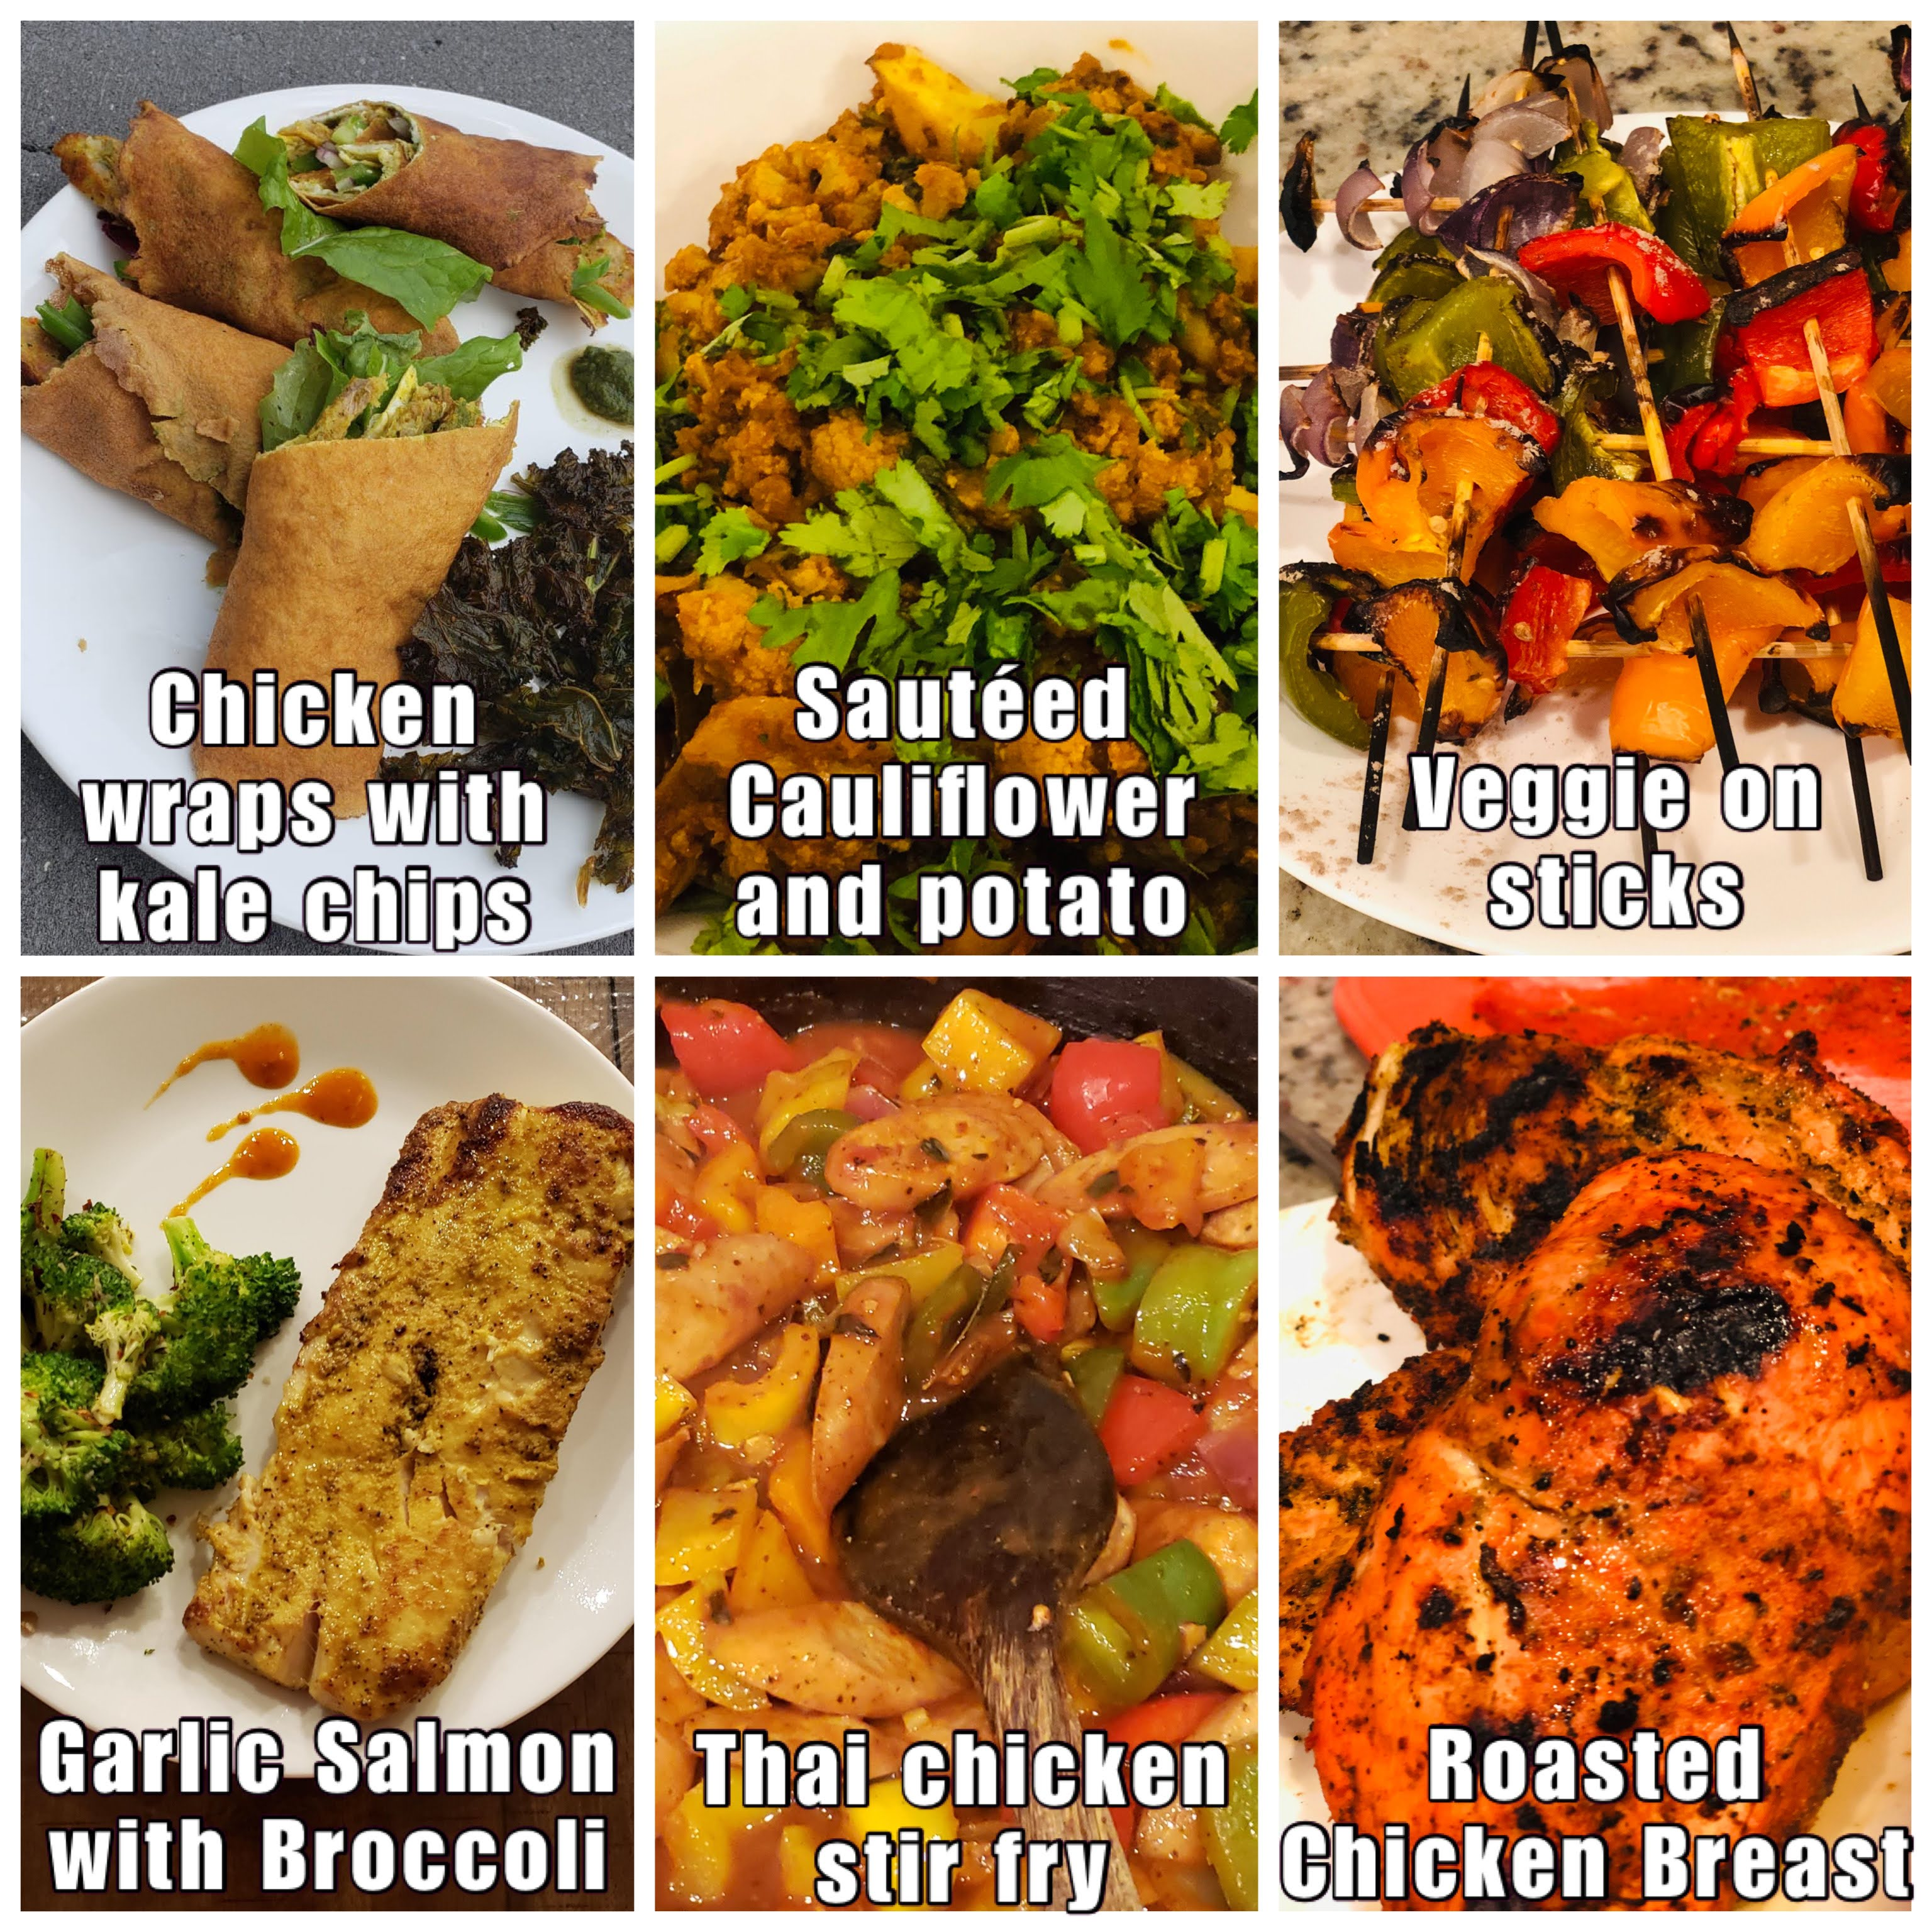
\includegraphics{pictures/dinner1.JPG}
\caption{A clean dinner}
\end{figure}

\begin{figure}
\centering
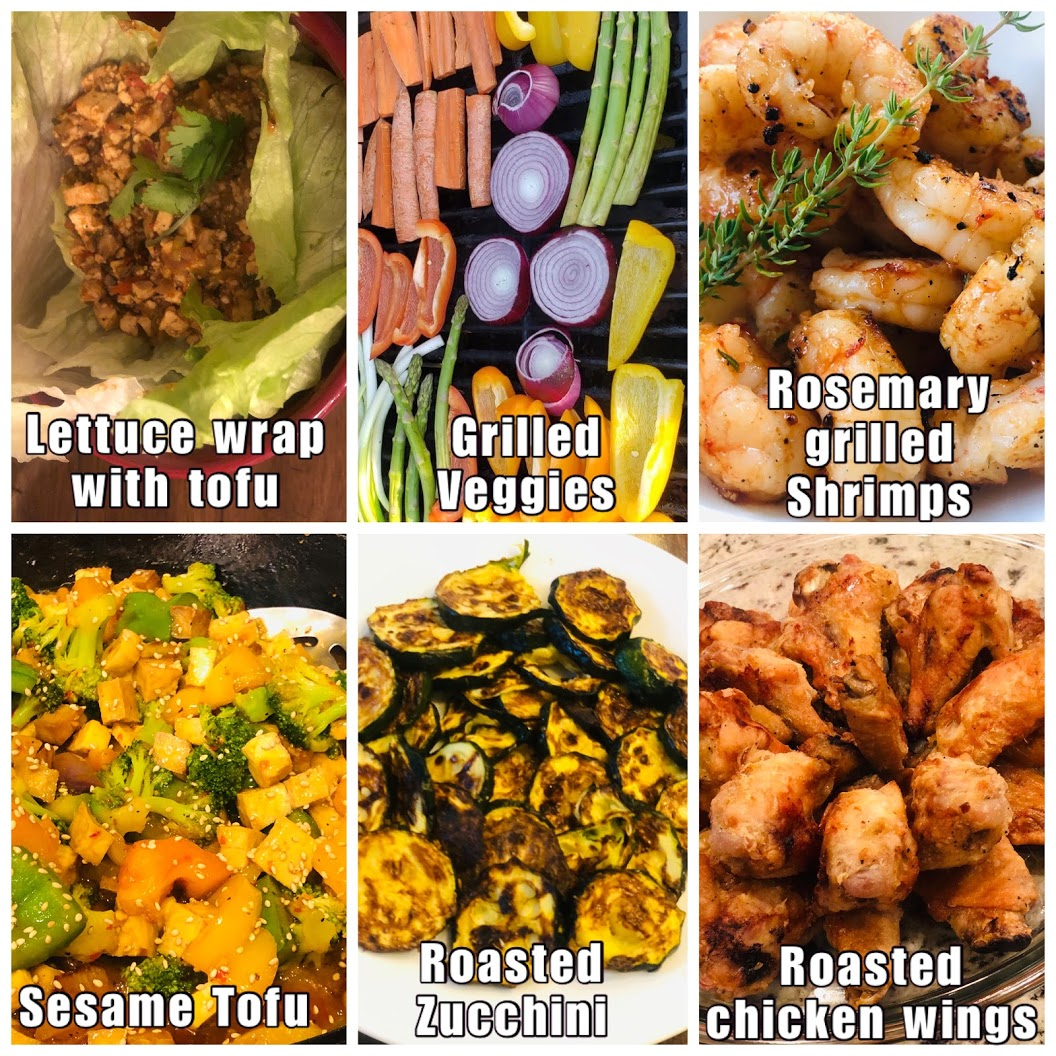
\includegraphics{pictures/dinner2.JPG}
\caption{More clean dinner}
\end{figure}

\pagebreak

\hypertarget{the-results}{%
\section{The results}\label{the-results}}

The following charts show our progress in terms of weight loss, with the clean eating periods highlighted. We did a clean eating in February-March and then another in July-August.

We saw very good results in both the iterations. The first iteration produced much better results because obviously there was just too much weight to lose, but surprisingly the second iteration was also very effective. The way we see this now is that if we ever hit a really long plateau in the journey to achieve the desired weight, we could just toughen our minds and do this again. It cannot hurt.

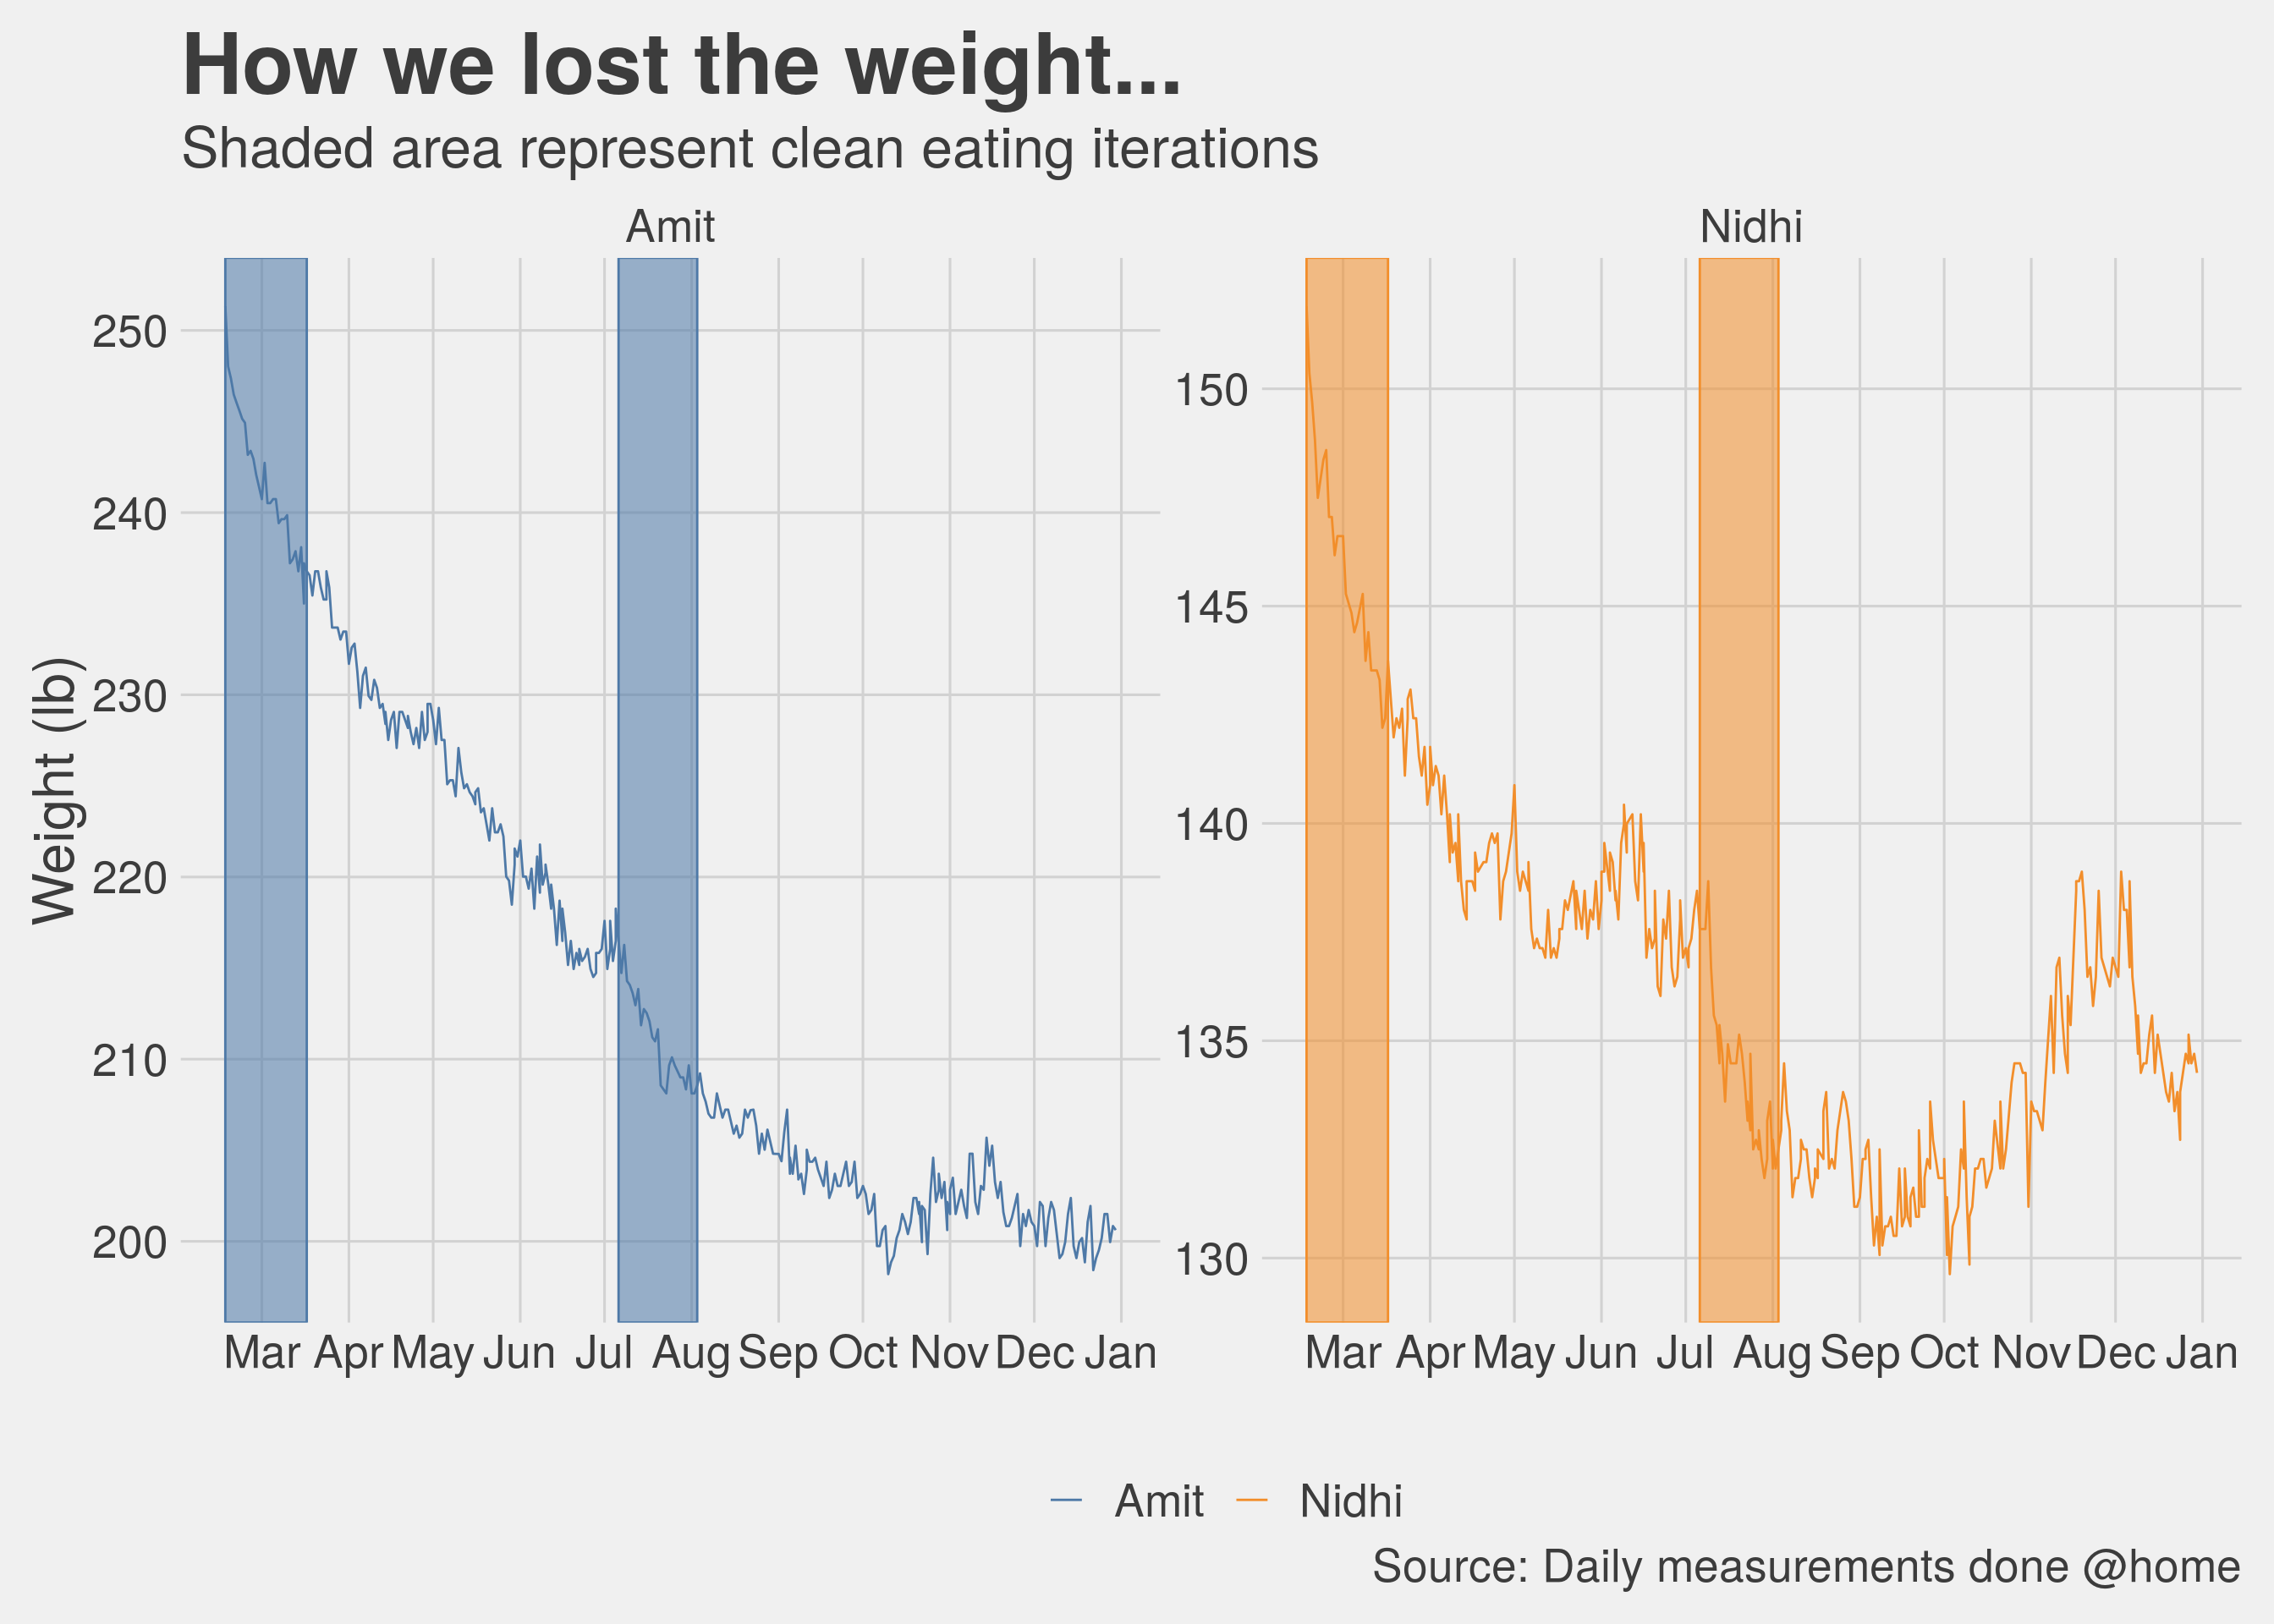
\includegraphics{bookdownproj_files/figure-latex/unnamed-chunk-5-1.pdf}

Here is another chart that compares the weight loss during clean eating and non-clean eating days. Note that even when we were not doing clean eating, we were still careful about what we were eating (in other words we were not gorging on Pizzas and butter chicken, soft and hard drinks were still completely off limits).

The chart shows a boxplot representing the spread of the weight loss per day during clean eating periods and non-clean eating periods. The horizontal line inside the box represents the median value of the distribution. For example, I lost at least 0.435 pounds per day on 50\% of the days during clean eating whereas I only lost at least 0.005 pounds on 50\% of the days during non-clean eating period. The data for this chart includes both clean eating periods over a timespan from 2020-02-17 to 2021-10-09.

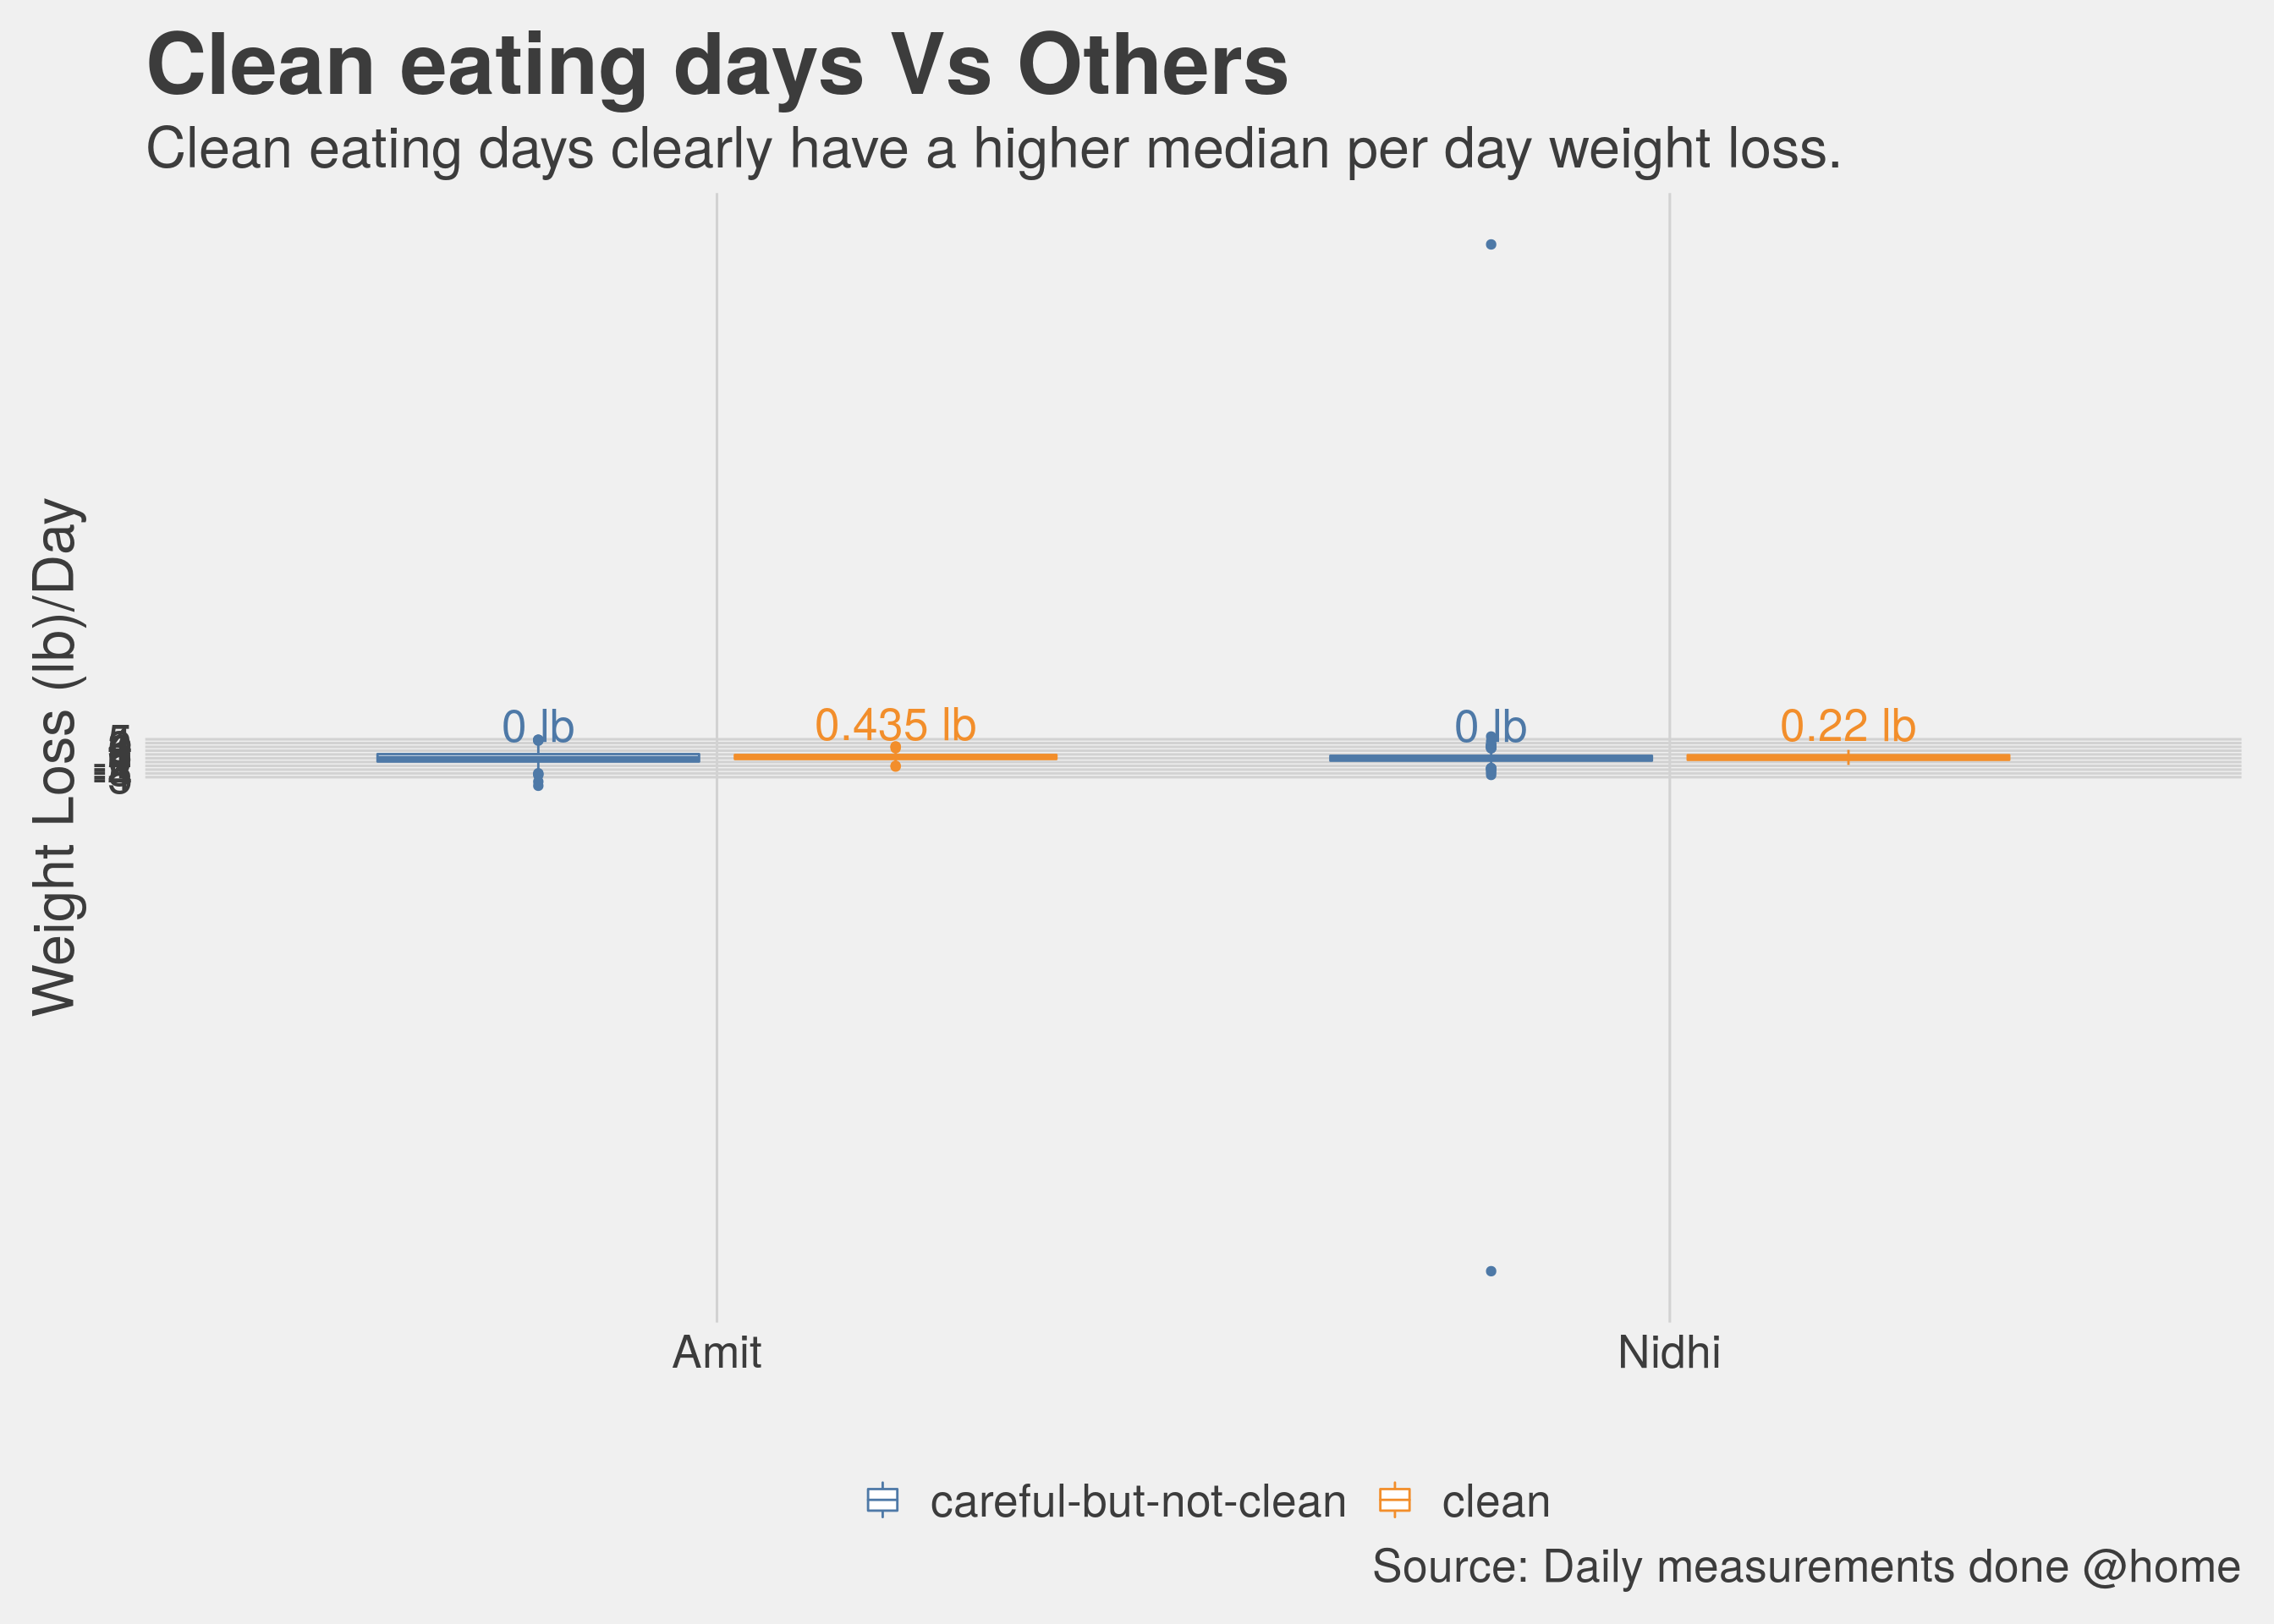
\includegraphics{bookdownproj_files/figure-latex/unnamed-chunk-6-1.pdf}

\hypertarget{is-the-30-day-challenge-hard}{%
\section{Is the 30-day challenge hard?}\label{is-the-30-day-challenge-hard}}

It is not very hard, certainly I did not feel it was, BUT tedious and tiresome is how I would describe it. It must be said though, it is hard for the chef for sure, our food menus did change. The fact that there isn't a restriction on eating vegetables or fruits makes it easier than other diet programs that I know of. It is a given that you are not eating potato fries daily for lunch or a mango as an after-dinner dessert every night. What makes it hard is that after the first few days the enthusiasm begins to wane, and the new eating habits take some time to become friendly. Once you adjust, both body and mind, to the new eating regimen then it does not feel like a diet at all. It certainly helps to have a goal in mind and keep reminding yourself why are you doing this.

For me, I think after two weeks or so, I could certainly start feeling the benefits, I felt lighter, more energetic (no late afternoon energy crashes), better quality of sleep, just overall lot of positives. While all this is happening, an interesting incident occurred. We had to be at a friend's place for a birthday dinner, the host was gracious enough to prepare some salads for us and we also took our own food with us. Midway through the party, I suddenly started feeling uncomfortable. The smell (aromas) of all the food and more so the alcoholic drinks made me feel nauseous, I felt like throwing up. Fortunately, I did not throw up and we had a very enjoyable evening other than those 30 minutes. I was totally fine when we were back home, totally fine the next day as well. It must be that 3 weeks into clean eating the internal circuitry in my body had maybe begun to rewire itself, or so I thought.

Another thought that often came to my mind was that good food is a source of happiness, of joy. The sweet gulps of the \href{https://en.wikipedia.org/wiki/Lassi\#Mango_lassi}{mango lassi} soothe the soul, the tangy and crisp \href{https://en.wikipedia.org/wiki/Panipuri}{Gol Gappe} tickle the brain, a \href{https://en.wikipedia.org/wiki/Paratha}{raddish or carrot or onion paratha} satiate the stomach like nothing else, and what even comes close to a \href{https://en.wikipedia.org/wiki/Butter_chicken}{butter chicken}? This is all true, however, food does not have to be the ``only'' source of happiness. There is happiness to be derived from good health, from feeling light, awake and agile throughout the day. A round of vigorous exercise resulting in a body drenched in sweat and a rush of endorphins is also happiness. Give it a chance, it will not disappoint you.

\hypertarget{what-happens-after-the-30-day-challenge}{%
\section{What happens after the 30-day challenge?}\label{what-happens-after-the-30-day-challenge}}

Several people have asked me, ``like other diets, do you go back to your old weight after you stop clean eating?''. My answer is ``yes, most certainly'' and this should not be a surprise. While I would not call clean eating a ``diet'', it is certainly accurate to say that there is no such thing as a ``one-time fix''. If you want the effects to be permanent then the lifestyle changes also must be permanent, there are no quick fixes. I have often heard in other contexts that being fit/healthy/strong requires a lifestyle change. I agree, it certainly does. Does it mean we can never eat unhealthy food? No, it does not mean that either. What it does mean is that you first become healthy enough and consistent enough with your nutrition and fitness so that a vacation, social gatherings or just plain eating out does not have to be viewed as a reason to say ``Oh, I need to workout extra tomorrow to burn all of these extra calories, or I need to fast for a day now\ldots{}'', your regular fitness and eating regimen is able to take care of it.

As our 30-day challenge was coming towards an end I was very much looking forward to eating a lot of Indian delicacies, all in one meal. I did that, probably having deprived myself a lot, I went overboard. The results were not pleasant. After about an hour, I started feeling miserable. I felt bloated, tired, lethargic and sleepy. For a moment I could not understand what was happening, sounds like an exaggeration but I had almost forgotten what it felt like to overeat. Nidhi then pointed out it was probably because of all the food I ate, that made total sense. I felt so full, I did not eat anything in the afternoon, nothing in the evening for dinner either. Next morning, I felt much better. This was my body's way of telling me that you do this again and I am going to react to this as if there is an alien invasion and the planet is in danger. Make no mistake, I have not stopped eating that food, I just eat smaller portions of it because I realize that what follows the 30 minutes of pleasure is several hours of unpleasantness.

\hypertarget{a-post-2020-update}{%
\section{A post 2020 update}\label{a-post-2020-update}}

We did not repeat the clean eating challenge again in 2021. Not because it was not useful anymore but because, it is a tool in the toolkit for attaining a healthy body weight, but it is not the only tool. Like all useful tools, it needs to be used judiciously. By the end of 2020 we understood to a good extent what kind of foods suited us, how are bodies reacted to certain food and so did not have the need or to a great extent the drive to do the challenge. The clean eating challenge at its core, is an exercise in finding out the relationship the body has with various kinds of foods by the process of elimination.

What we were now figuring out was something that can be described as ``infinitely sustainable''. Chapter 11 of this book discusses this in detail. Also, as 2020 was ending and the festival season was approaching, clean eating challenge was no longer on our minds and then in 2021 we started experimenting with other things such as water fasting. So, while we still eat reasonably clean (no soft drinks, minimal hard drinks either, minimal processed foods or sugars) doing the clean eating challenge again is not high on the list.

\hypertarget{chapter-4-at-a-glance}{%
\section{Chapter 4: At a glance}\label{chapter-4-at-a-glance}}

\begin{center}\rule{0.5\linewidth}{0.5pt}\end{center}

\begin{enumerate}
\def\labelenumi{\arabic{enumi}.}
\item
  The 30-day clean eating challenge is a way to detox your body by staying away from any and all processed food and especially processed sugar.
\item
  We mostly ate a diet high in protein, fiber and good fats. This meant we remained full for a longer time and were able to eliminate snacking and surprisingly (for us) did not experience cravings for any specific food item.
\item
  The two times we did the 30-day clean eating challenge we saw an increased weight loss per day on an average.
\end{enumerate}

\hypertarget{exercise-putting-in-the-hard-yards}{%
\chapter{Exercise: Putting in the hard yards}\label{exercise-putting-in-the-hard-yards}}

You would have probably heard that managing weight is 70\% about nutrition and 30\% about exercise. I think this correct. Having said that, we should not downplay the 30\% i.e.~the exercise. As I have mentioned earlier in the book, a few years back I tried a purely diet-based plan and achieved good results. The problem with it, like with all diet based plans, was that it was not sustainable. There is another aspect to this as well, when I tried losing weight purely via the diet route (a.k.a. counting calories) my overall appearance became thinner or to use the more appropriate term here, weaker. While I do not recall feeling lack of energy, but the appearance was as if I had just lost a lot of weight from sickness and it did not look healthy. Several people asked me out of genuine concern if I was sick and when I told them that I was doing this diet their reactions were on the lines of ``ok, but don't do more of it''. This time however, things are different, both me and my wife look leaner and fitter. Our body structure has become ``denser'' if that is the right word to use here and it is because of that we look thinner and fit into much smaller clothes. Appearance wise we do not have the starved look that I suppose comes from severe calorie restricted diets. Without a doubt, this is the result of the rather intensive exercise routine that we now have.

\hypertarget{counting-calories-and-why-it-does-not-work}{%
\section{Counting calories (and why it does not work)}\label{counting-calories-and-why-it-does-not-work}}

If you have ever made a conscious effort to lose weight, chances are that you are aware of the phrase ``counting calories'' or ``caloric restriction''. These phrases refer to the idea that we note the calories we expect to get from the food items we eat and once we know that we restrict our daily caloric intake to a number lesser than the average recommended value (see the FDA guidelines \href{https://www.fda.gov/media/112972/download}{here}). The idea being if we eat less than what our body requires then the body ends up burning stored fat reserves, ergo, we lose weight. The problem with this approach is that while the idea is correct, but it is not sustainable. You can lose weight by consuming less calories than what your body needs based on your specific life circumstance but then for how long? Nobody like to be deprived of foods they love (I am not suggesting we surrender to cravings for junk food that are specifically engineered to trigger those cravings), keep feeling hungry or worse feel stressed because we are not able to consume (in appropriate quantities) foods that we like. Think about it, if calorie counting worked then someone in the past 100 years would have figured out a way to make it work in a sustainable fashion, we know by looking all around us that it is not the case.

There are two things to understand here, a) calorie counting is a tool, it is a way of measuring how much is enough and b) not all calories are the same. When we are eating processed food, getting a realistic count of calories is difficult. The amount of energy that our bodies have to expend to metabolize processed food is much less than the amount of energy required to get the same number of calories from whole foods, thus the cost per calorie in terms of calories burnt and calories gained is much smaller for processed food. Put simply, processed food is going to make us fat, fast!

What if we were able to burn more calories rather than having to eat less food? This is where exercise and specifically strength training comes in. When we do strength training consistently over months and years, we build muscle and the body then has to keep burning fat (even when we are at rest) to generate calories to sustain these muscles. A balance of eating healthy and strength training regularly is what helps to ultimately find that fine equilibrium, just as Goldilocks found the porridge that was just right. It is important to mention that just as caloric restriction is not the panacea, the idea that ``I can eat anything now that I work out 5 days a week'' is also incorrect and most likely harmful in the long run even though it might prevent weight gain in the short term.

\hypertarget{there-is-always-a-first-time}{%
\section{There is always a first time}\label{there-is-always-a-first-time}}

When I went to the gym for the first time this year, it was not just the first time for me in the year 2020 but it was for the first time in my entire life of 41 years. I had no illusions of how supremely unfit I was and how difficult this was going to be. Sometimes, I used to see people exiting after their class and I used to tell myself ``OK, that person looked great, but that is probably because he has been working out since forever''. Of course, this may or may not have been true, but my goal was to keep telling myself that if I was disciplined enough to show up rain or shine and do the exercises as told then I would get better, that is just how it works (at least that is what I told myself anyway).

I look at some old videos now of me doing exercises like planks or air-squats when I started, and I compare them with the more recent ones of me doing the same exercise. My movements used to be very clumsy, almost hilarious, and it is to the credit of the trainer that she did not give up on me. Nidhi on the other hand, being a dancer, her movements had a natural rhythm, she had flexibility and havingdone some exercises while growing up, she was much more comfortable with the whole setup. My objective was not to be as good as her but to simply by better than me from four weeks ago. Here is a picture of me doing squats, about a year apart. The one on the left is my attempt to do a squat with a box to support in case I fall, the one the right is me doing the same exercise but this time with a 45lb kettlebell and heels elevated on a plate. Doesn't even look like the same person, does it :). Procrastination is the absolute worst thing we can do, no matter how uphill a battle it appears at the start, it is always the first step that lays the foundation and it is consistency that creates the stairway to success.

\begin{figure}
\centering
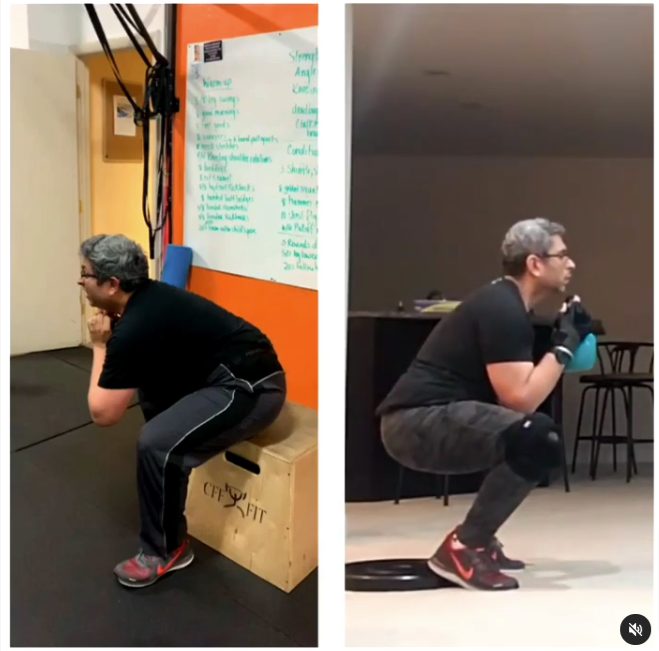
\includegraphics{pictures/goblet_squat_w_kb.png}
\caption{Goblet Squats}
\end{figure}

We started with working out twice a week, and then went to thrice, and then four times and now I work out five times a week. Nidhi tried the four times a week routine but is now nicely settled into three times a week. In about 8 months I went from having to push myself to work out twice a week to now chasing endorphins. Of course, it helps that because of Corona, we are all working from home so we have a little more flexibility with our schedules. If there was one silver lining that I could find in that otherwise disaster of a year, it was that we could fit in time for self-care.

One day a couple of months into training, I stumbled upon a YouTube video of the training routine of an actress who played the role of a superhero in one of her movies. Her trainer said when she came to the gym and looked at people doing pullups and deadlifts, her reaction was that ``Oh yeah this is cool, and all but I can't do that'', and a few months later she was deadlifting 235 pounds. When I saw the video, I had a similar reaction. I thought sure, a Hollywood actress with a celebrity trainer can of course do this, I cannot. I WAS WRONG. I recently deadlifted 325 pounds, and while I still do assisted pullups, I can at least visualize myself doing some real pullups by myself, not easy, but possible.

I am hugely inspired when I see a video of an athlete's working routine, a movie star spending weeks and months in the gym training for a role to look the part or just so many people who share fitness content on social media. Like everything else, social media also comes with its share of the good, the bad and the ugly, it depends upon you which lens you choose to view the world.

\hypertarget{our-workout-routine}{%
\section{Our workout routine}\label{our-workout-routine}}

I am not a personal trainer; therefore I am not qualified enough to talk about the technical details of what makes for a good workout but I would like to share what we did and loved.

Our workout sessions were an hour long and were mostly divided into five parts:

\begin{itemize}
\tightlist
\item
  Warm up (about 5 minutes)
\item
  Strength (about 10 to 15 minutes)
\item
  Strength \& Conditioning (15 to 20 minutes)
\item
  Core (5 minutes)
\item
  Stretches (2 to 3 minutes)
\end{itemize}

With some rest time and setting up equipment for different exercises the above routines added up to an hour (give or take 5 minutes). From mid-January when we started to about the end of March we were working out twice of week in our trainer's gym and since then we have been working out at home and our home gym has slowly metamorphosed from being your amateur home gym to a souped up version with lots of weights, barbell, deadlift equipment, resistance bands, boxes, pull up bars, rowing machine etc. Some of the stuff we bought, some our trainer was kind enough to lend us for a while (because Corona). Here are a couple of pictures.

\begin{figure}
\centering
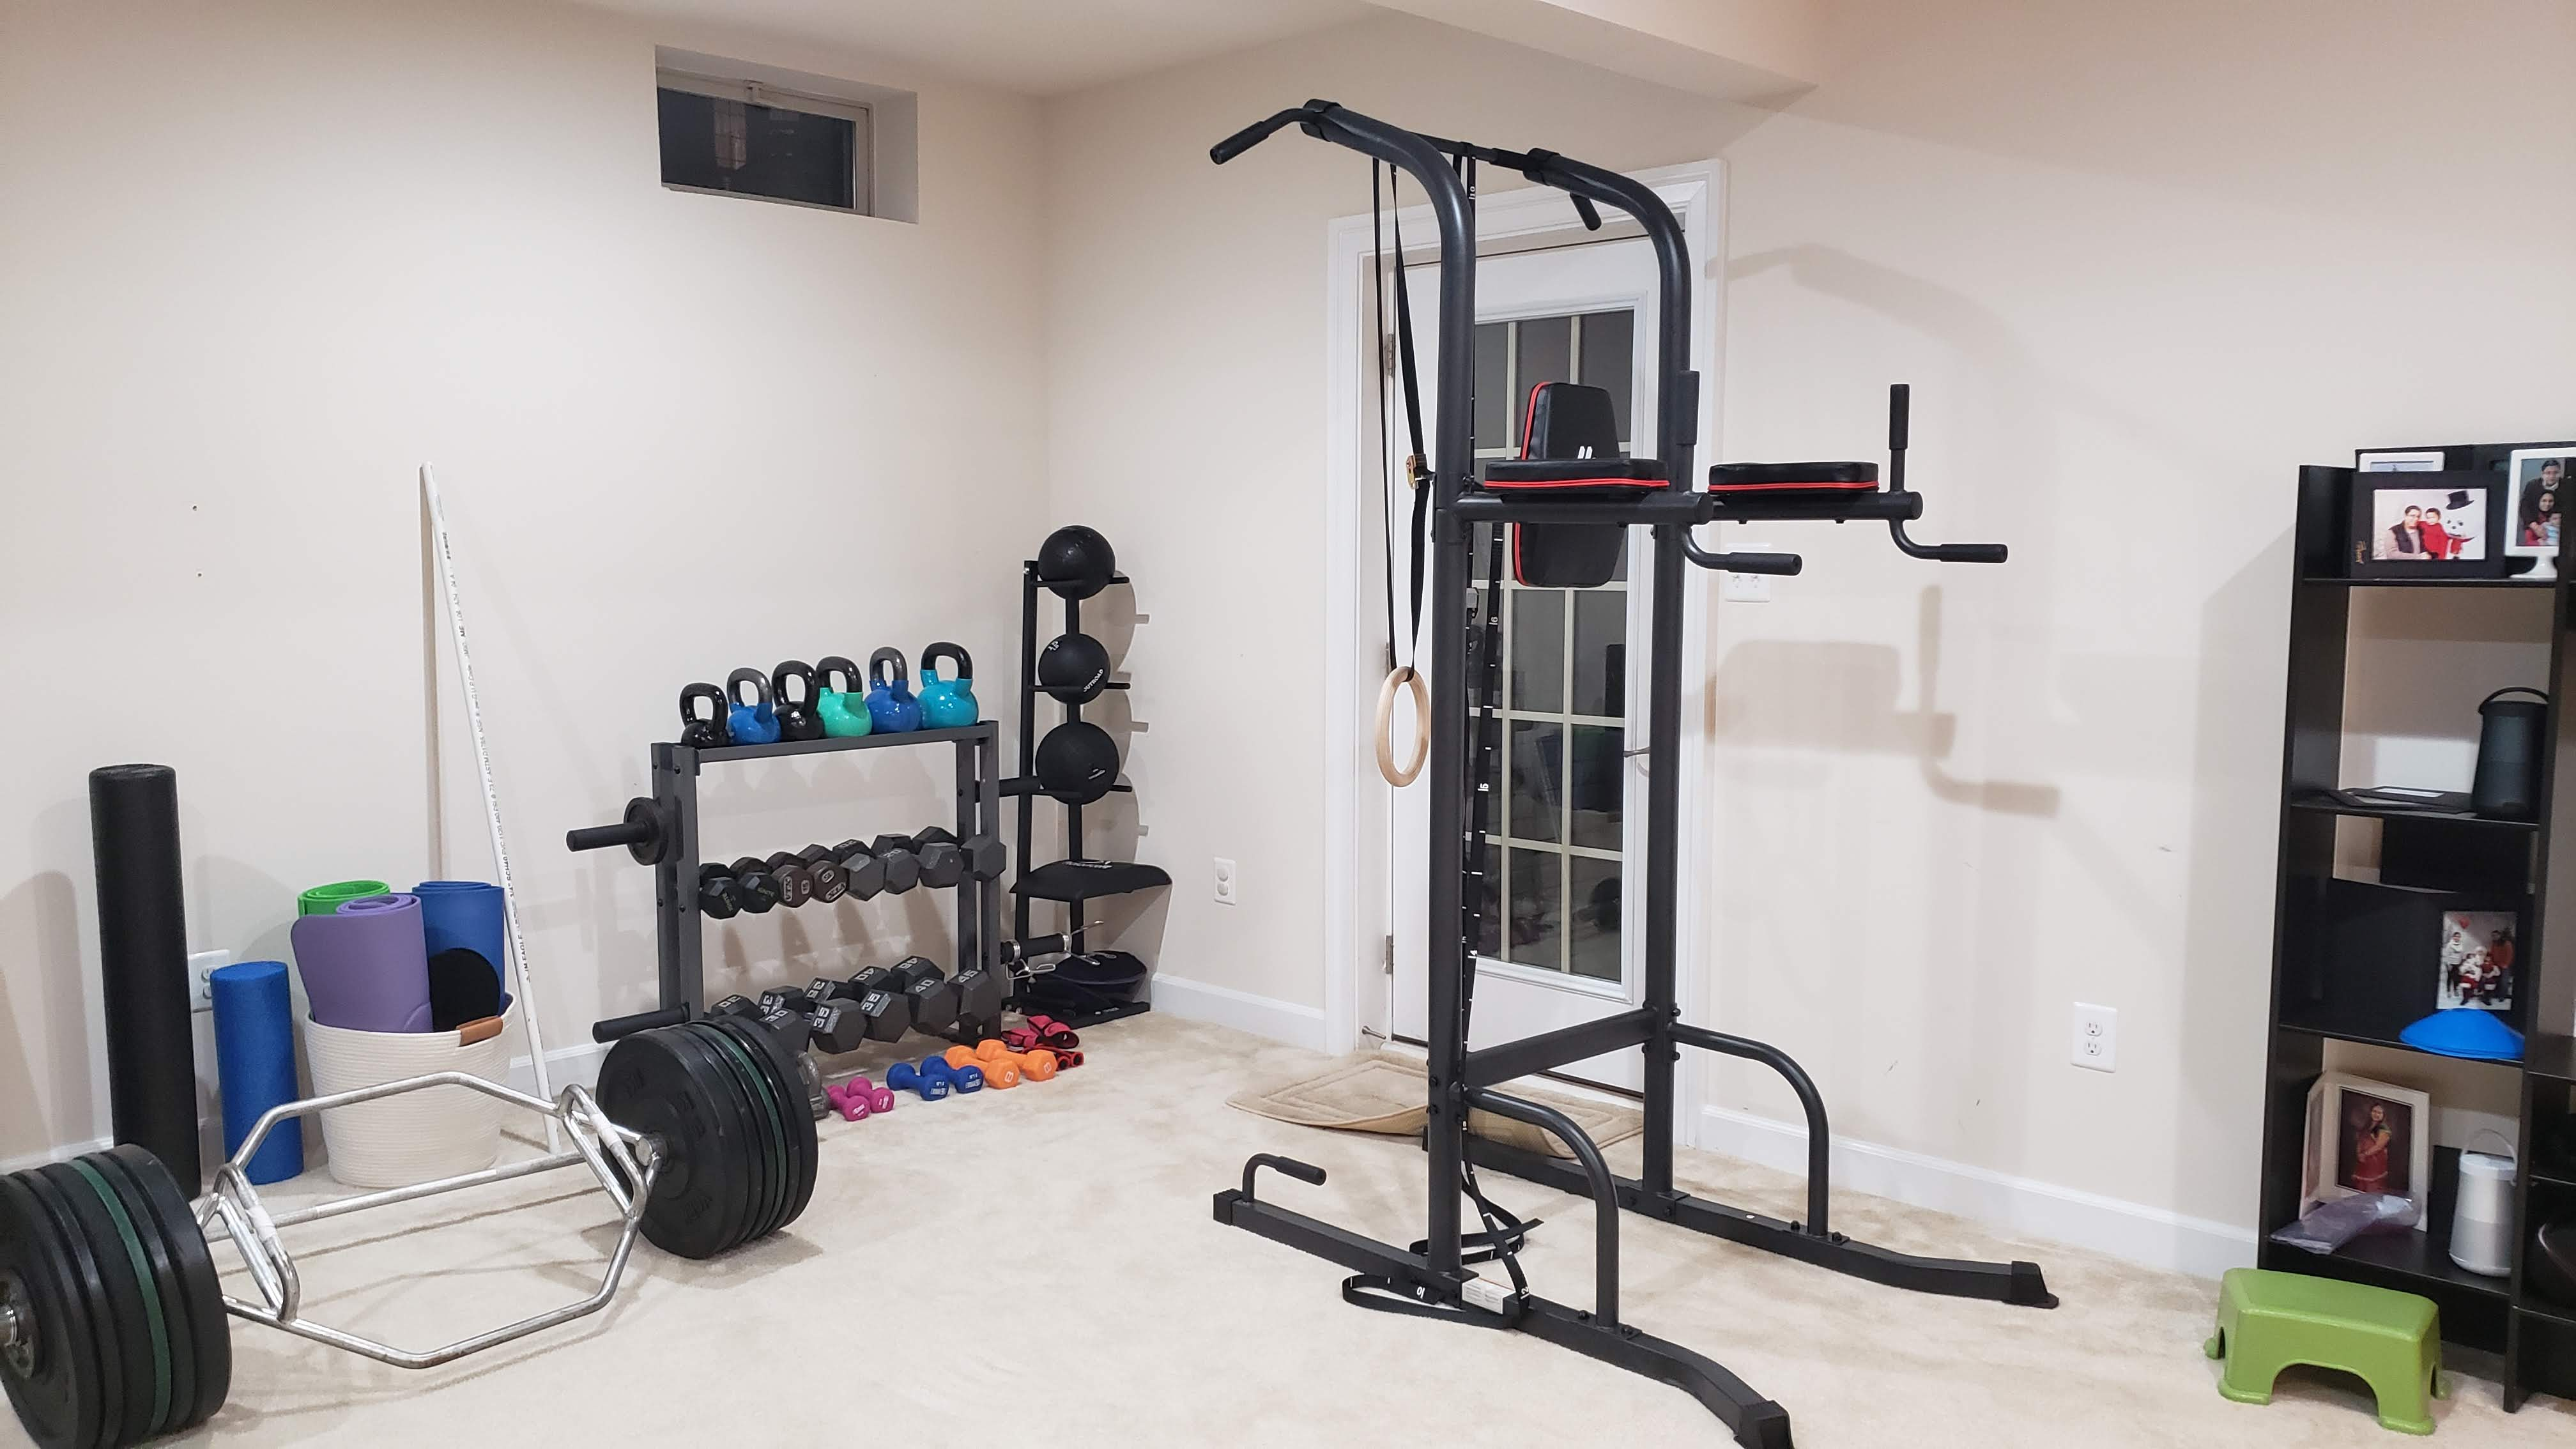
\includegraphics{pictures/gym2.jpg}
\caption{Weights and such}
\end{figure}

\begin{figure}
\centering
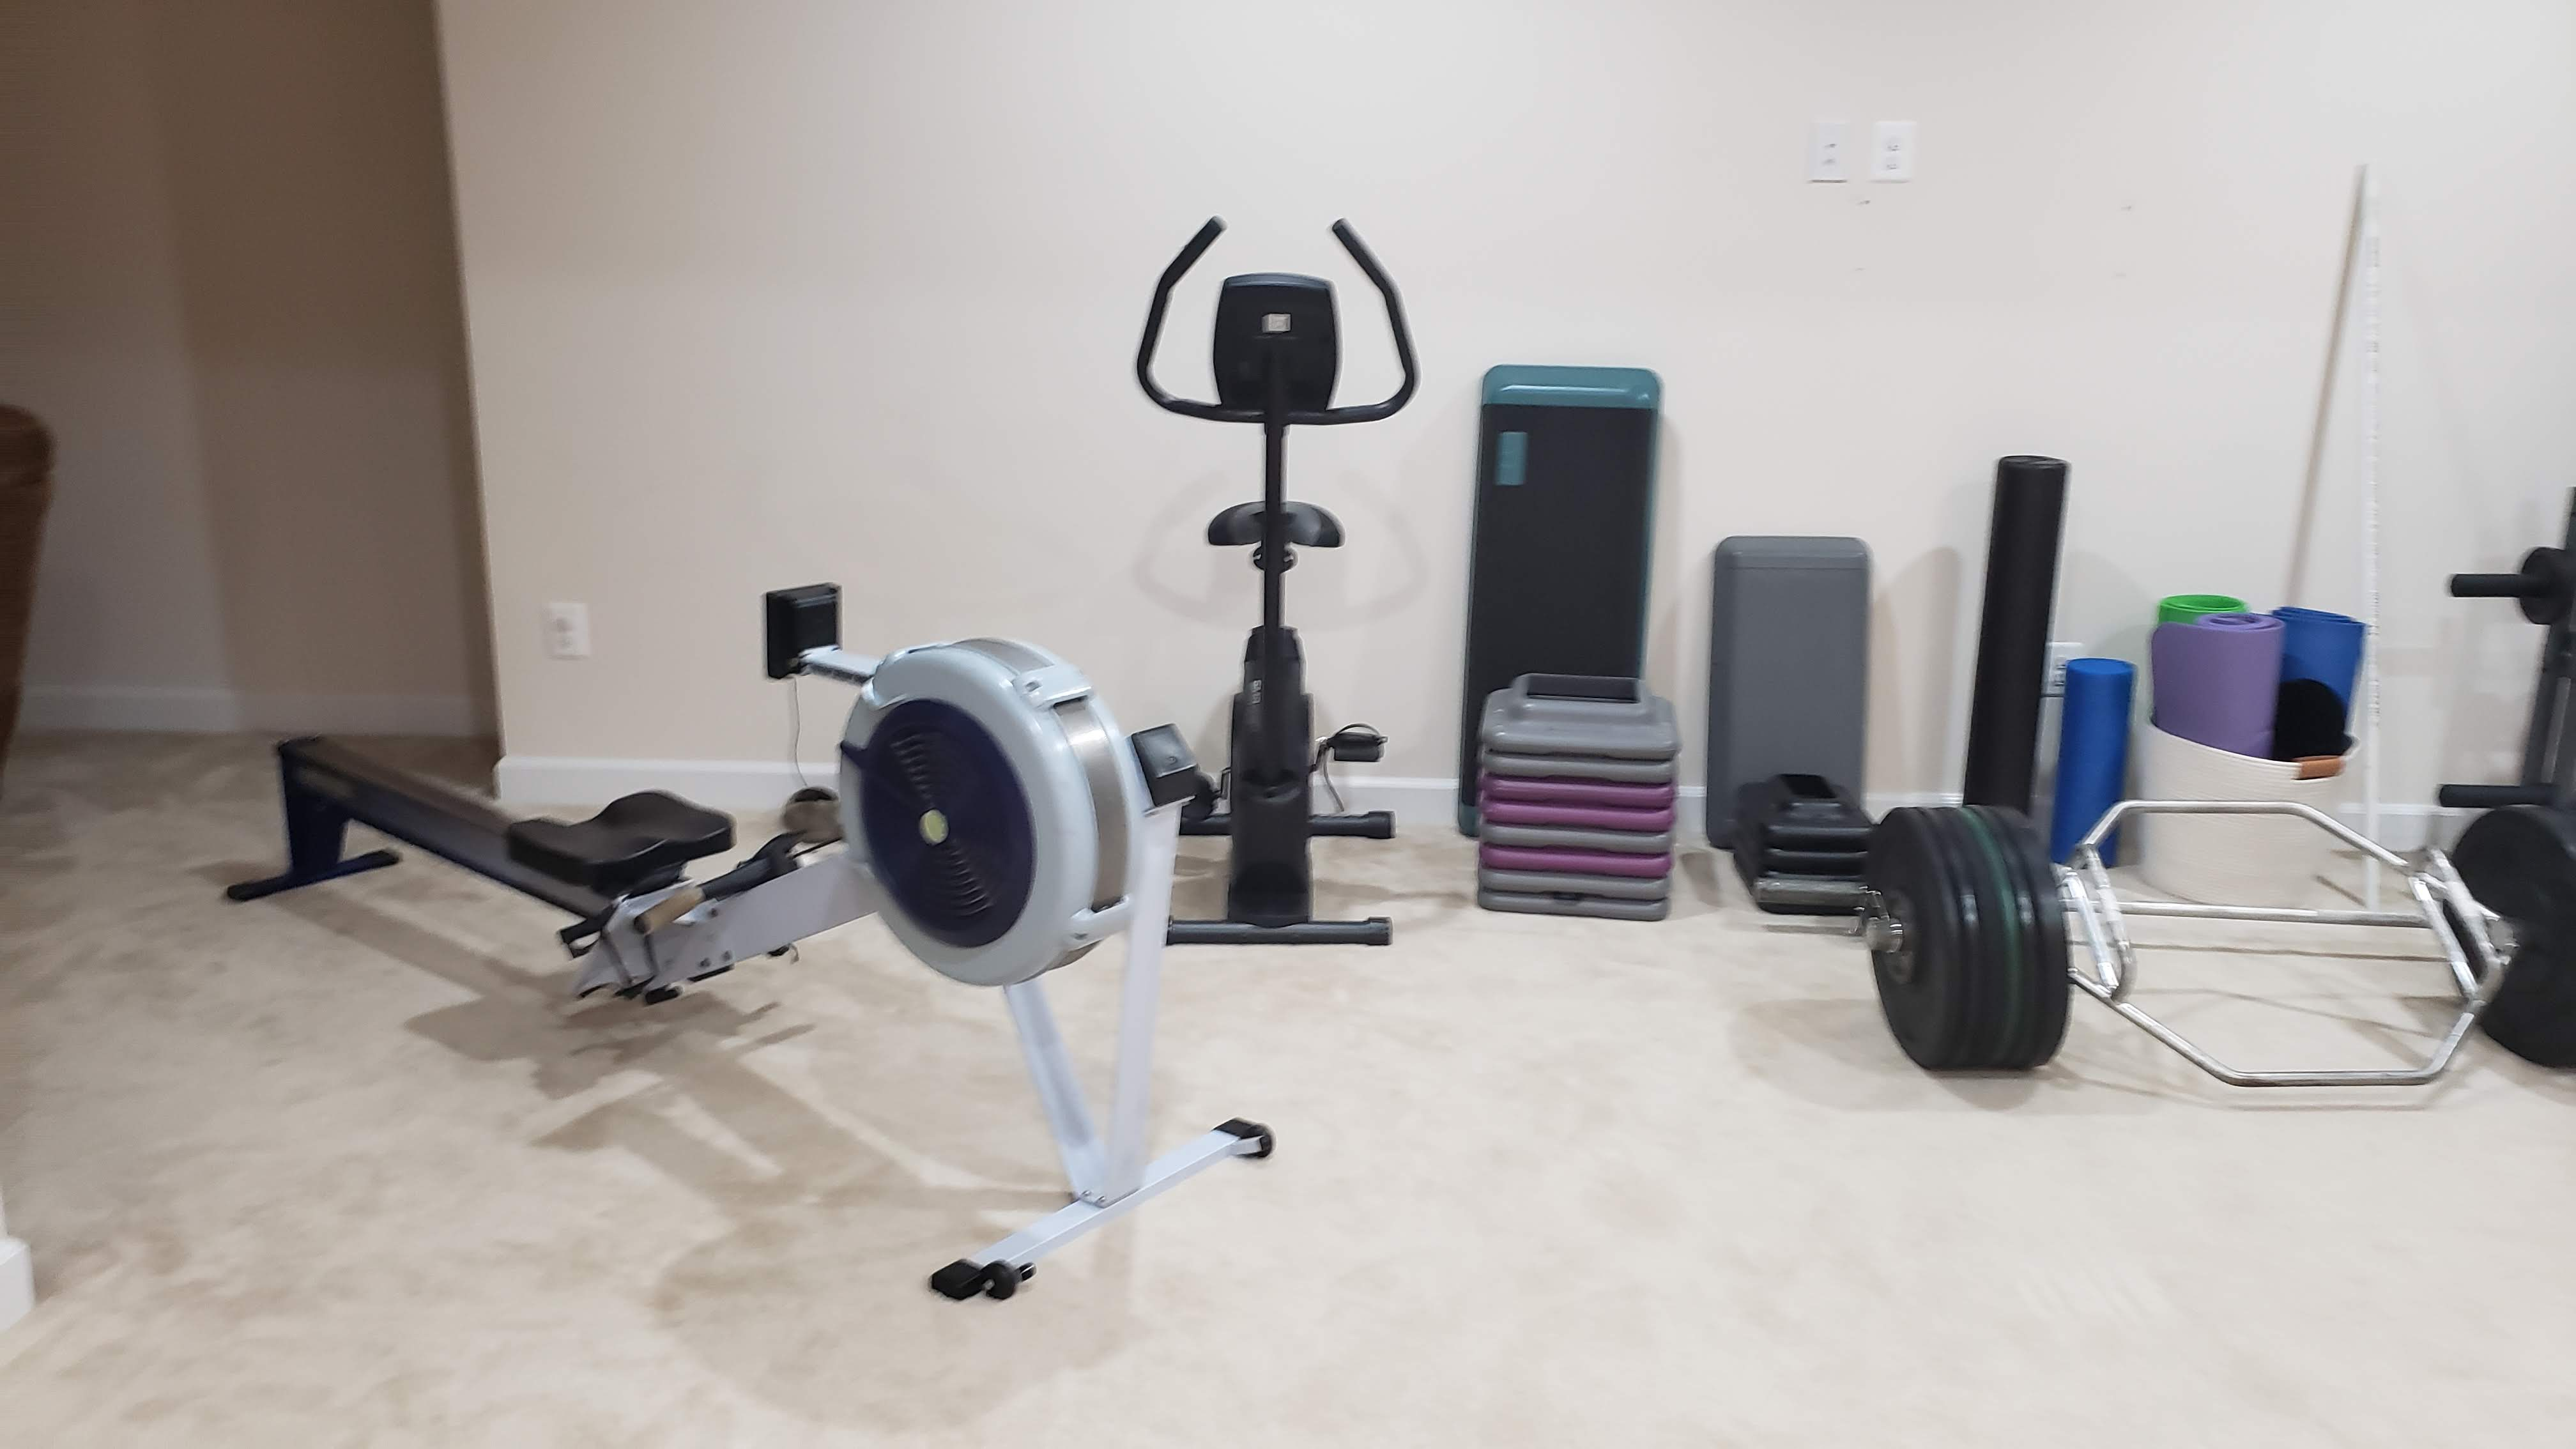
\includegraphics{pictures/gym1.jpg}
\caption{Rowing machine and cycle}
\end{figure}

For a long time, I used to tell myself before the workout, that warmups are easy, the strength portion is just 10 to 15 minutes so it will be over quickly before I realize and then the conditioning is the only part that I have to push through and then by the time I am half way through the conditioning it would be almost over and then the core is super easy (it really isn't). This kind of mental setup helped me get through the hour. Of course, once I was in the middle of it, unless the workout on the day absolutely pulverized me, my mind used to blank, barely any thoughts at all. This thought process has changed over time, now I enjoy the workouts, my mind and body are now used to the fact that for the next 45 to 60 minutes I would experience physical stress (not physical pain, just controlled stress) and that is OK and expected. Post that stress would be a feel-good period, a calm mind and sharp focus.

I have experienced this several times when I used to work out in the afternoons or evenings that going into the workout from a crisis at work is a huge mental shift. Once the workout is over, I realize that maybe the work problems were not that insurmountable as they appeared an hour back. It could be the exercise, or just the fact that I have had the opportunity to (forcibly) extricate myself from the crisis and now after an hour I am able to think more clearly. I do not know what the reason is, but I do know that I experience mental clarity after the workout.

The following tables show a subset of the different exercises we did, over time, as part of the warmups, strength, conditioning and core. These were done over a period, with the more difficult ones such as the Turkish getup added much later and for the ones which we did from the start we kept on increasing the weights or the numbers of sets and reps over time.

The complete list of exercise is huge, there are just so many of them, we kept meticulous notes of what exercise we did and weights we used for those exercises (wherever applicable). The purpose of putting this list here is to emphasize two things, firstly a good training routine requires a lot of different exercises to train the big muscles, the small muscles and everything in between and secondly this is not DIY, there is a lot of thinking and planning that goes on before we show up in the gym that is done by our trainer. It is similar to a conversation I once had with my dentist about flossing my teeth, I asked her ``so which teeth do I need to floss?'', and she replied rather nonchalantly ``only the ones you would like to keep\ldots{}''. It is the same with muscle groups.

At the same time, I do not want anybody who works out at home on a treadmill or a spin bike or goes out for a run or does any other form of exercise to see the following tables and feel overwhelmed. Any which way you get your 150 minutes per week of moderate intensity physical activity (\href{https://www.cdc.gov/physicalactivity/basics/adults/index.htm}{CDC guideline}) is good. The more I think about it, the more I feel that we just organically fell into this routine. It was as if we found this beautiful path through the woods, decided to explore it further and loved every step of the trail.

One last point before ending this section, keeping track of your workouts is super important to see how you are progressing (not so much for the pace of progress but simply to know that there is progress, or not). However, this is hard to do manually and after a period simply impossible to do manually. There are some good apps out there which you can use, choose something that allows you to export all your data out so that you are not tied to that one app but can actually see the raw data for yourself in a spreadsheet.

\captionsetup[table]{labelformat=empty,skip=1pt}
\begin{longtable}{ll}
\toprule
\textbf{Exercise} & \textbf{Body part/Muscle Group} \\ 
\midrule
Shoulder CARS & Shoulders \\ 
Trunk Rotations & Hips, lower back \\ 
Trunk Swivels & Hips, spine \\ 
Squat to stiff legs & Hamstrings \\ 
Birddogs & Core, spine \\ 
Quadruped shoulder rotations & Shoulders \\ 
Star Pushups & Shoulder \\ 
Banded butt bridges & Glutes \\ 
Easyseated forward folders & Hips \\ 
PVC zott squats & hips, glutes \\ 
PVC dislocates & Shoudlers \\ 
Lying Ys and Ts & Shoulders \\ 
Banded clamshell raises & Quads, hips \\ 
Bretzel & Quadsm shoulders \\ 
 \bottomrule
\end{longtable}

\captionsetup[table]{labelformat=empty,skip=1pt}
\begin{longtable}{ll}
\toprule
\textbf{Exercise} & \textbf{Body part/Muscle Group} \\ 
\midrule
Deadlift & Posterior Chain \\ 
Squat into press & Quads, shoulders \\ 
Pushups & Chest \\ 
Strict Press & Shoulder \\ 
Kettlebell Swings & Posterior chain \\ 
Turkish Getup & Shoulders and core \\ 
Back squats & Quads, glutes \\ 
Overhead tricep extensions & Triceps \\ 
Hammer curls & Biceps \\ 
Hexbar carries & Posterior chain \\ 
Quarter landmines & Shoulders \\ 
Chinup holds & Biceps, shoulders, core \\ 
Calf raises & Legs \\ 
 \bottomrule
\end{longtable}

\captionsetup[table]{labelformat=empty,skip=1pt}
\begin{longtable}{ll}
\toprule
\textbf{Exercise} & \textbf{Body part/Muscle Group} \\ 
\midrule
Weighted Squat Jumps & Quads, glutes \\ 
Straight arm lateral pulldowns & Lats \\ 
Wall sits with ball at chest level & Quads, glutes \\ 
Single arm push press & Shoulder \\ 
Skull crushers & Triceps \\ 
Push press & Shoulder \\ 
Goblet squats & Quads, glutes \\ 
Pullups & Biceps, lats \\ 
Burpees & Whole body \\ 
Body rows & Lats, biceps \\ 
Pistols & Glutes, quads \\ 
Close grip bench press & Chest, triceps \\ 
 \bottomrule
\end{longtable}

\captionsetup[table]{labelformat=empty,skip=1pt}
\begin{longtable}{ll}
\toprule
\textbf{Exercise} & \textbf{Body part/Muscle Group} \\ 
\midrule
Palloff press & Abdominal muscles, shoulders \\ 
Palloff circles & Abdominal muscles, shoulders \\ 
Bicycles & Abdominal muscles \\ 
Tricycles & Abdominal muscles \\ 
In and outs & Abdominal muscles \\ 
Planks & Abdominal muscles \\ 
Plank circles & Abdominal muscles \\ 
Plank walkups & Abdominal muscles \\ 
Hip dips & Abdominal muscles \\ 
Alternating V-ups & Abdominal muscles \\ 
Pilates pump & Abdominal muscles \\ 
Iso crunches & Abdominal muscles \\ 
Mountain climbers & Abdominal muscles \\ 
Kneeling dumbbells around the world & Abdominal muscles \\ 
 \bottomrule
\end{longtable}

The conditioning part of the routine usually consisted of either a 15-minute AMRAP (as many rounds as possible) or a 12-minute EMOM (every minute on the minute) or sometimes a HIIT (high intensity interval training) such as Tabata or on some days just a combination of exercises.

\hypertarget{our-calendar-so-far}{%
\section{Our calendar so far}\label{our-calendar-so-far}}

The following charts shows the calendar for the year 2020 and 2021 with the days we exercised marked with an {[}E{]} and the amount of weight lost/gained reflected by the color. Red indicates weight loss and green indicates weight gain. More ``red'' than ``green'' in a month means overall, we lost weight in that month. I like this chart a lot because it brings out very clearly that weight loss is never a straight line, you gain some (days) and you lose some (days), except in this case, losing is better.

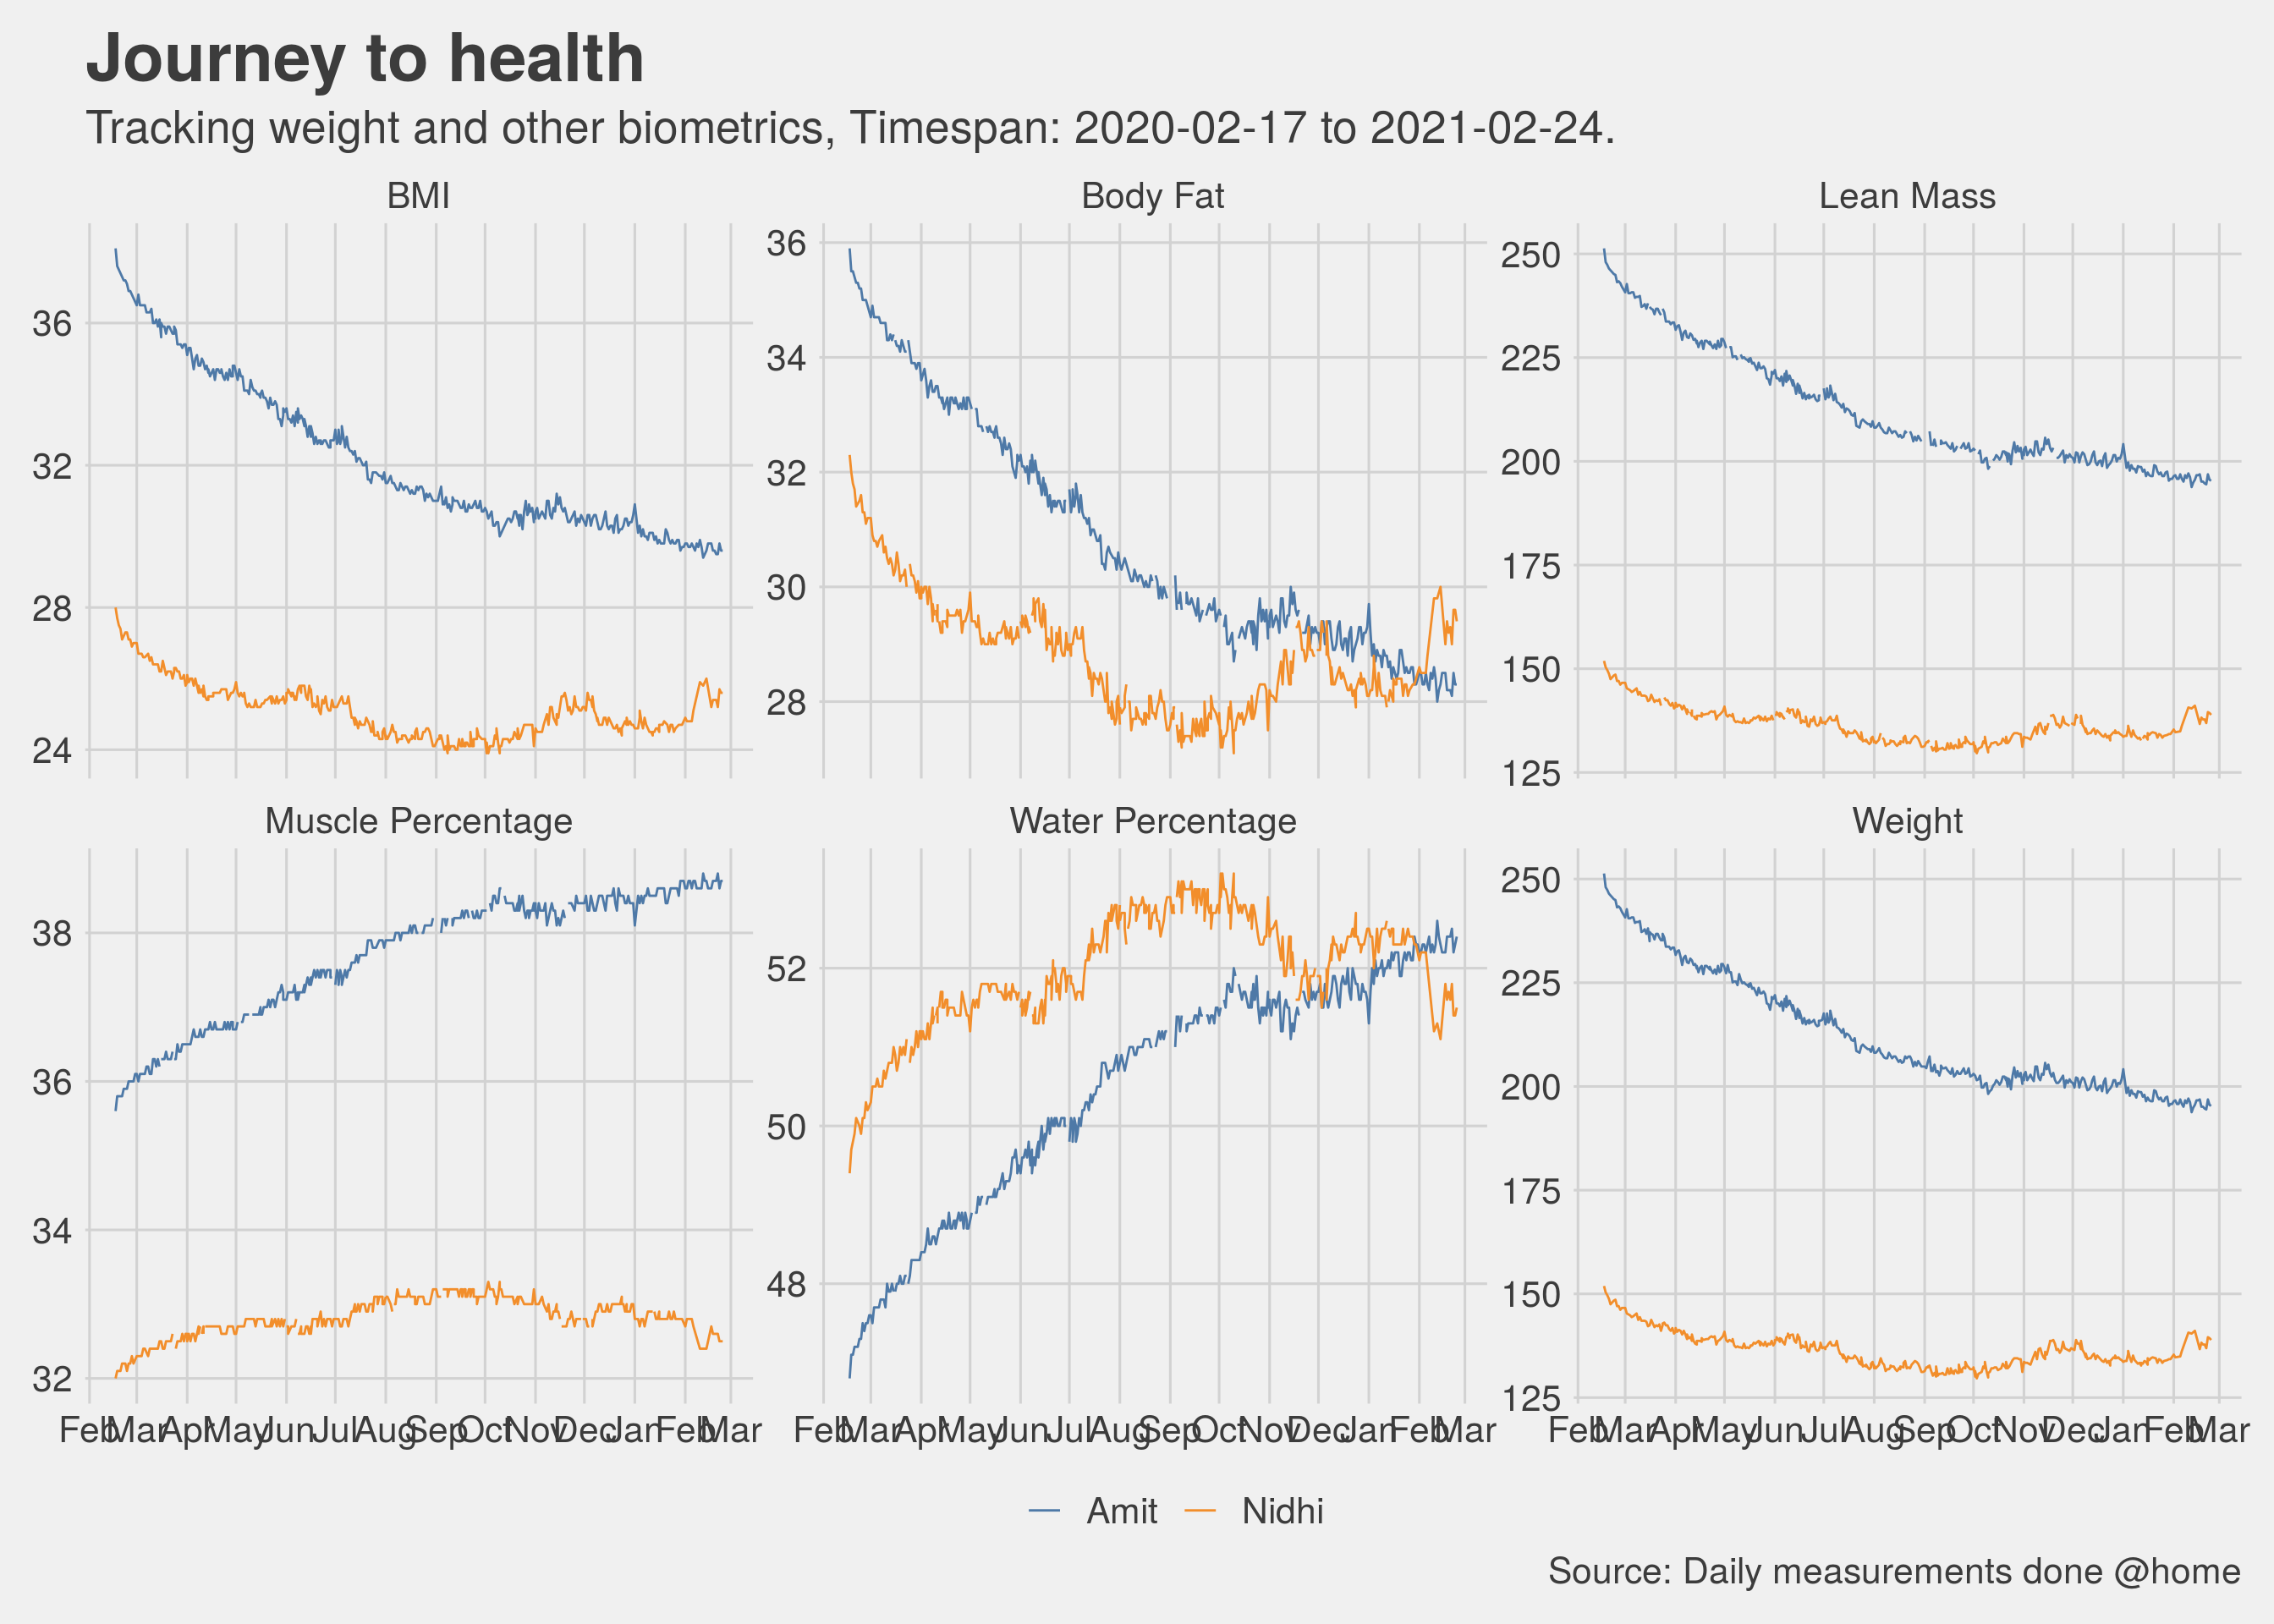
\includegraphics{bookdownproj_files/figure-latex/unnamed-chunk-12-1.pdf}

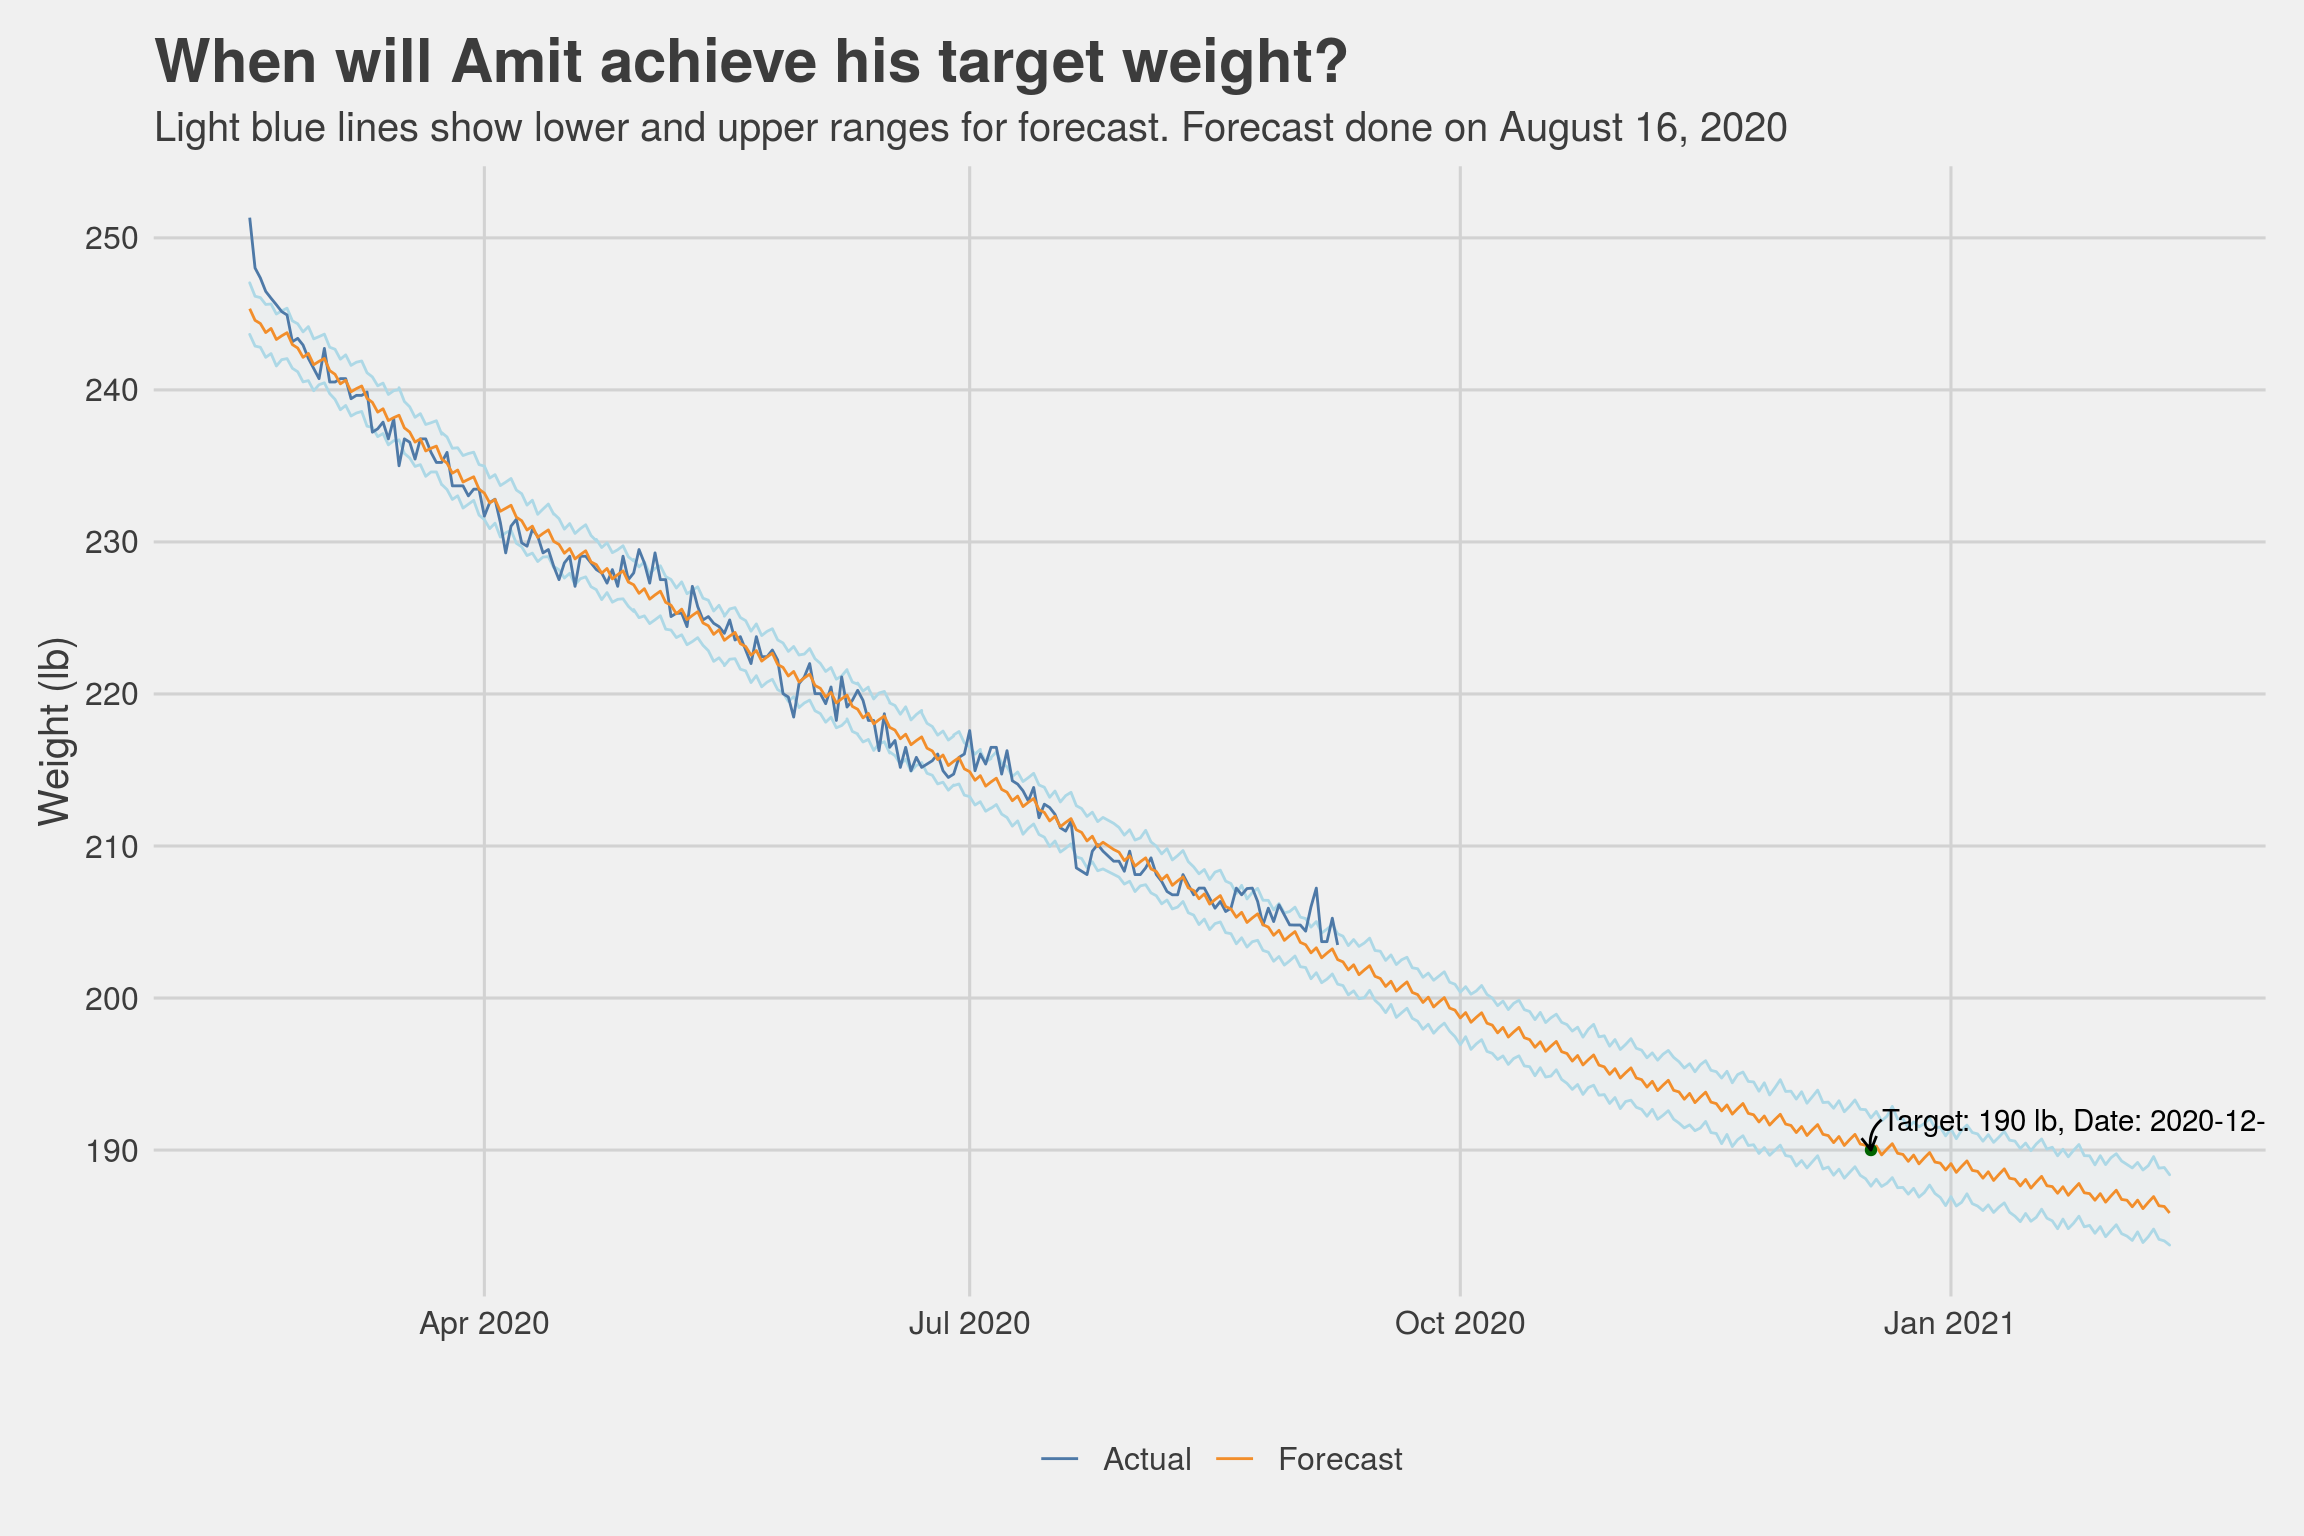
\includegraphics{bookdownproj_files/figure-latex/unnamed-chunk-13-1.pdf}

You can notice in the charts the number of days marked as {[}E{]} (for exercise) has increased over the months in 2020 until August and from that point on it was settled at 5 days a week or 20 days a month for me and 3 days a week or 12 days a month for Nidhi. As we exercised more and ate right, the body became stronger and it could take on more work and so we exercised even more, it became a self-propgating cycle. Exercise also gives you a ``high'', a feeling of euphoria, you cannot miss it. Stated differently, this increased number of workouts, doing more sets and reps, this was only partially driven by just the motivation to lose weight, the rest of it was because A) the body became strong enough that the current load became easier and so a step up was needed and B) the desire for that ``high'', it makes you want to get more of the stuff that got you here in the first place. If this book ever gets into the hands of someone who has exercised for any length of time, I would like to add that what I have written here may seem routine and totally on expected lines to you but to me this was unlike anything I had experienced before, it was a joyous discovery. Lookup \#chasingendorphins on Twitter or Instagram and you will see what I mean.

\hypertarget{that-which-does-not-kill-us-makes-us-stronger}{%
\section{That which does not kill us makes us stronger*}\label{that-which-does-not-kill-us-makes-us-stronger}}

*Quote from Friedrich Nietzsche

Deadlifts are my favorite. They are a full body exercise; our trainer says deadlifts are a game changer. I have watched a lot of celebrity trainers on YouTube and heard them echo the same sentiments. While we did several different variants of the deadlift such as the single leg stiff leg deadlift, the sumo stance deadlift etc. but my personal favorite and something that I religiously tracked was the deadlift with a hexbar. Maybe it had to do something with the visual imagery I had in my head of this being a strong man's exercise. I remember that when I first saw the hexbar in the gym I asked our trainer when we would be using it and she said, you will get there in a couple of weeks (this was sometime in mid to late February). The hexbar weighed 55 pounds, it was the heaviest they had.

The first day I tried it, I recall that the trainer was very cautious, I don't know if she thought I could even do it (I was fat and never been to the gym until last 2 months remember, this was February). To this day, when I have graduated from lifting the hexbar with no weights to lifting the same hexbar with 135 pounds plates on either side, she is still extremely cautious and rightly so. My deadlift goal is 400lb, which as it stands of today (September 9, 2021) is 2.15 x my body weight. I currently deadlift 325lb which as of today is 1.74 x my body weight.

Is the 400lb or 2x body weight just an arbitrary tough ask for an ``alpha'' exercise such as the deadlift or a truly worthy \& aspirational goal for the ``king'' of exercises? Let me dwell on that number a little bit, where did this 400lb or 2x body weight goal come from? For me I believe it just came from the Internet, the usual fitness blogs, YouTube videos and the like. I have not come across a scientific study comparing the benefits of a 1.5x, 2x or say a 3x body weight deadlift. The Internet is filled with blogs from well-respected strength coaches about 2x being the right of passage to real strength goals. My personal opinion (my book, my opinions :)) is that if you are not an athlete and on the other side of 40, then being able to deadlift 2x is a remarkable achievement that isn't something most people you would meet in an year would be able to do! It takes a lot of sustained training to lift anything more than bodyweight, truth be told, for me even getting to deadlift equal to my body weight was a lot of work. Getting the form correct, getting the breathing right, getting every muscle group involved in the exercise stronger, getting the focus right, it all takes some amount of doing. Plus, there are highs, lows and plateaus, sometimes you just get stuck at a specific weight and need to change a few things in your technique to make progress or just wait it out.

A completely valid question that someone might ask is ``Why do I need to deadlift? I am not a power lifter, and this seems like it is a super specialized exercise.''. A rather unexpected answer would be that deadlift is not just a strength building exercise but also a rehab exercise for lower back precisely because it is a strength building exercise! Getting stronger is the best insurance against not getting injured, and this is true not just in the gym but also in life. All of us use and will continue to use our lower backs so strengthening it should not be considered as an optional nice to have. If you lift something from the floor you are using the same musculature that you would use when you deadlift, better strengthen that back.

The following two chart puts all this in perspective.

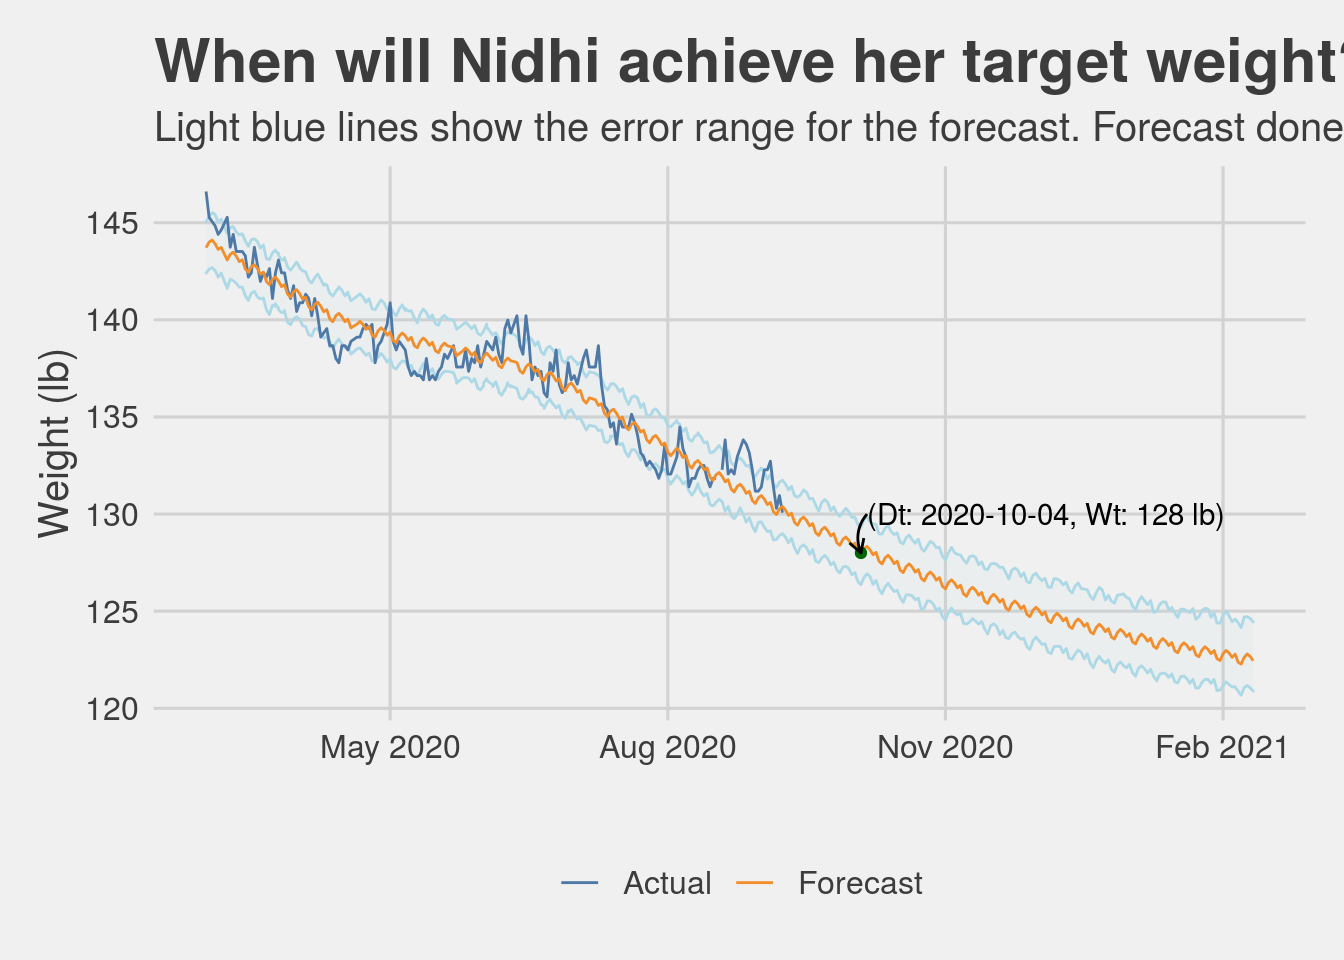
\includegraphics{bookdownproj_files/figure-latex/unnamed-chunk-14-1.pdf}

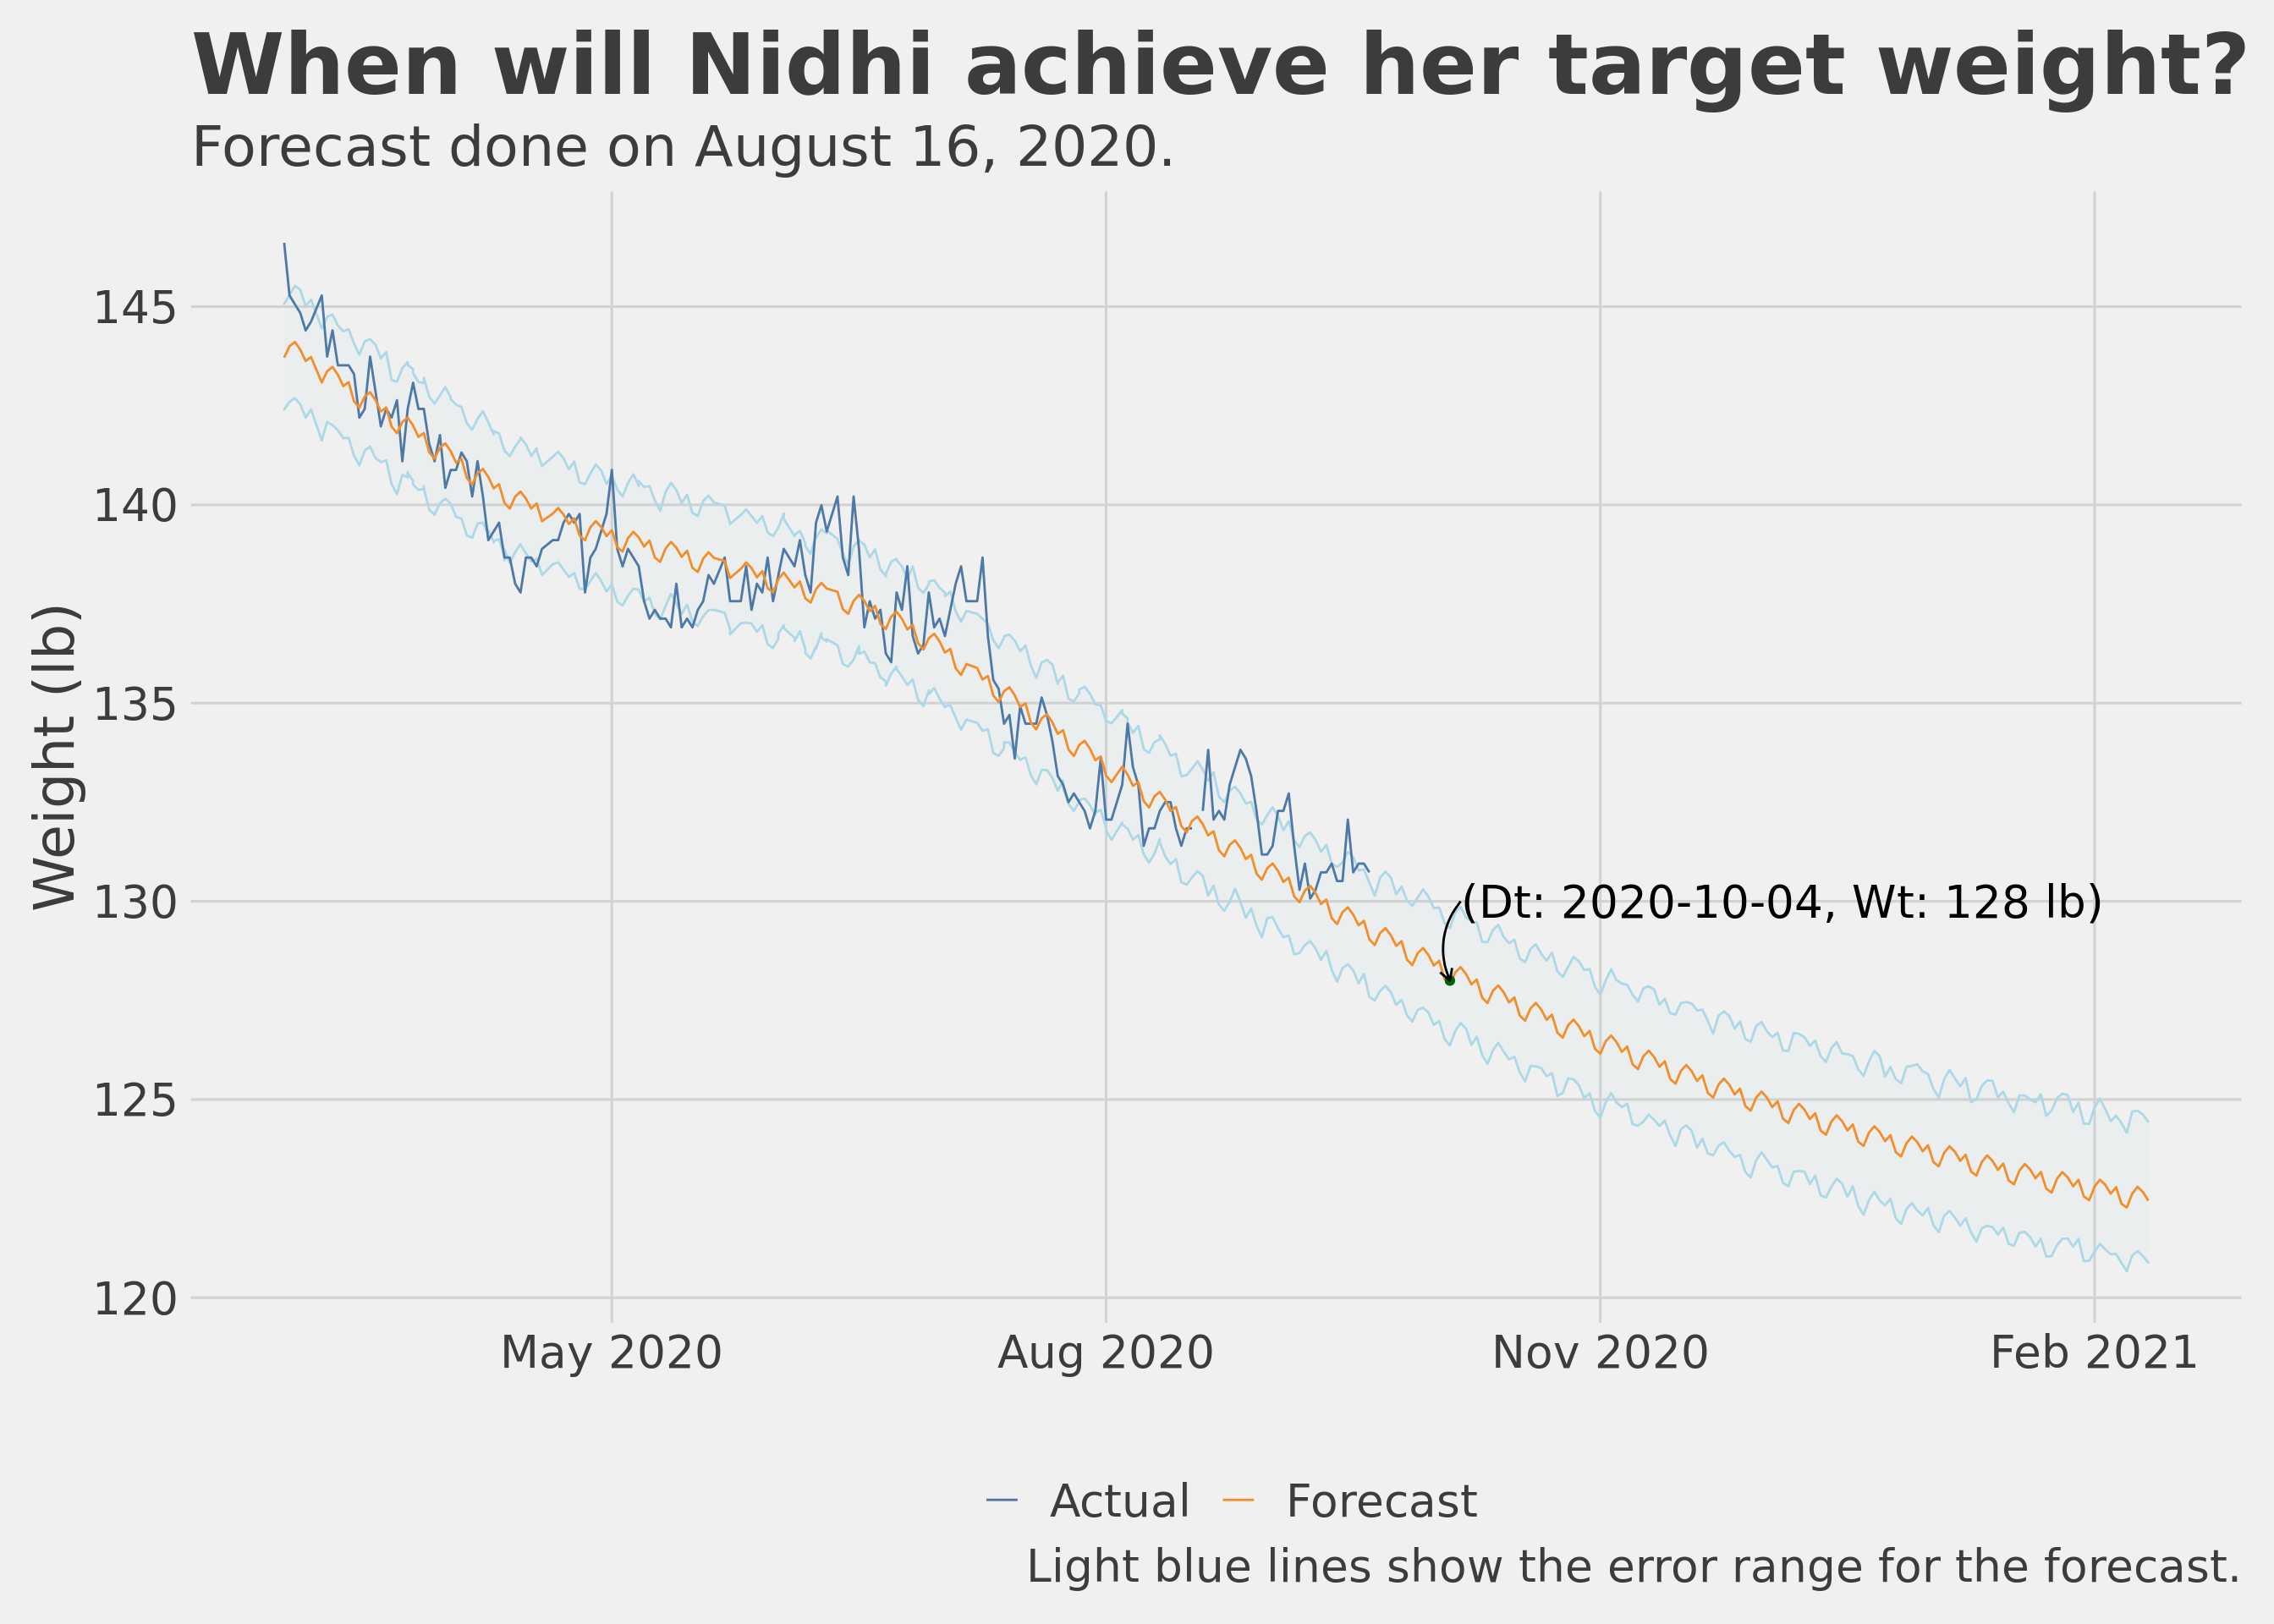
\includegraphics{bookdownproj_files/figure-latex/unnamed-chunk-15-1.pdf}

The key observations from the above charts are:

\begin{itemize}
\item
  It gets progressively harder. Took 7 months to get to 1 x bodyweight, 11 months to get to 1.5 x bodyweight and then a total of 19 months to get to 1.75 x body weight so lifting 325lb with a bodyweight of 185lb. I expect to be at 2 x bodyweight or 370lb in the next 4 to 6 months, so 2 years to get to lift 2 x bodyweight.
\item
  As I started losing weight, I was able to lift more weight. Not unexpected, as you get stronger you are able to lift more, makes sense. But now, I want to stay around 185lb bodyweight, otherwise the 400lb would be a challenge harder than what it already is.
\end{itemize}

Viewing this journey from a completely different lens and using the deadlift as a metaphor, I guess we should all try to find something that takes perseverance and hard work over a long period of time to achieve and then start on the road to achieve that. Over a period of time we will realize that the goal itself was simply an impetus to get started but as we keep putting in the hard yards and keep seeing the milestones along the way, those small hits of dopamine keep driving us forward. We live in a world today that is designed to provide instant gratification but rather provides years of compounded benefits, does indeed take some time to sink in.

PS: On December 22, 2021 I was able to lift 2x of my bodyweight, although not all the way off the ground but a plate elevated version where the hexbar is kept two inches above the ground making the lift a tad bit easier. Here is a picture of me lifting 385lb, my bodyweight that morning was 191.3lb.

\begin{figure}
\centering
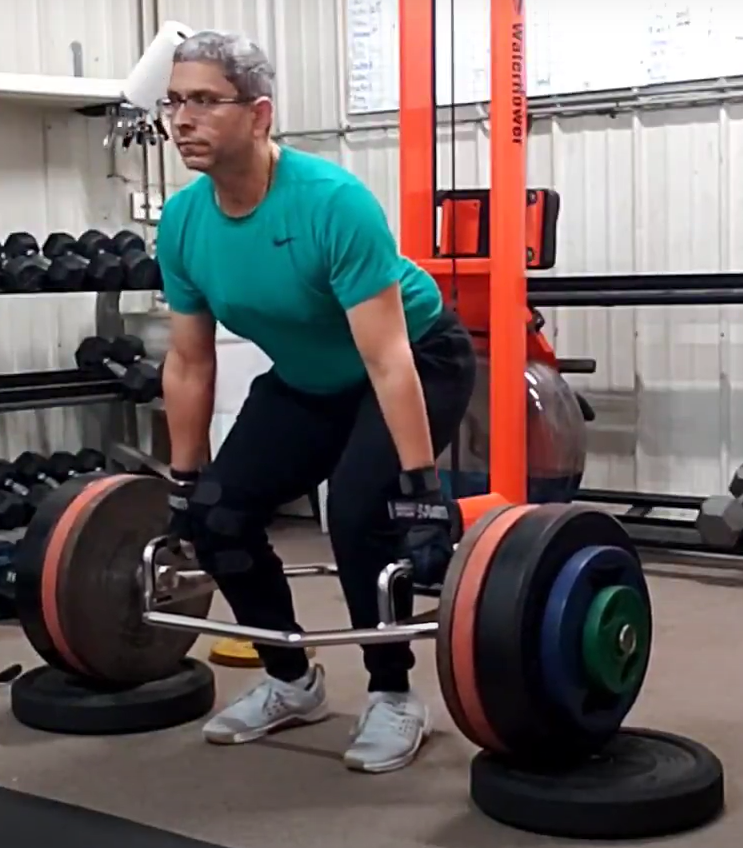
\includegraphics{pictures/385lb.png}
\caption{Hexbar, total weight 385 pounds}
\end{figure}

\hypertarget{do-i-really-need-a-trainer}{%
\section{Do I really need a trainer?}\label{do-i-really-need-a-trainer}}

Short answer: \textbf{Yes}. Longer answer: \textbf{Yes, please}.

We were very fortunate, and I certainly count it as a blessing that we were able to simply meet a wonderful trainer without having to find one. A kind-hearted, good natured person who just happens to be a fitness trainer walked into our lives when we decided to set sail on this journey. Maybe if we worked with someone else our experience would have been different. Given what we did experience, I would certainly recommend finding a good trainer. A good trainer is one who not only is an expert but more importantly makes you feel that they are personally invested in your success. That being said, there are other more technical reasons as well for why you should get a personal trainer.

DIY workouts are great but they could also be limited. You can buy an exercise cycle, maybe a rowing machine, an elliptical, or any of those one stop shop kind of machines and start working out on your own. Good for you. What I realized is that there is a lot more to workouts than just calorie counts. If your goal is something beyond just burning calories but to gain overall strength and build muscle (not to be confused with becoming a body builder) then you need to do a lot of different kind of exercises which work on different body parts and different muscle groups. This requires knowledge and expertise; it is not DIY. It is important that these exercises are done under expert supervision where a trainer is watching your posture, giving feedback and correcting you in real time. If you do not feel good with an exercise then a good trainer will suggest an alternate, there are just so many different things that come into play here as we experienced over the last several months. This idea that just because all knowledge is now simply a Google search away so everything is DIY does not apply here (or anywhere, in my opinion) and could even be dangerous in my opinion.

A good trainer will keep your long-term goals in mind and keep on evolving your workout to help achieve those goals. Goals here are not just in terms of weight but also in terms of let's say your cardiovascular strength. As your body starts getting stronger, the workouts need to adapt. For example, if you could do 3 rounds of 4 exercises in a 12-minute AMRAP today, then maybe in two months you should expect to do 4 or 5 rounds of the same (or an even harder) routine in the same time. A trainer would be able to gauge that and work with you to help achieve that. For myself, I have a goal of being able to deadlift 400 pounds, going from 200 to 400 pounds requires paying extreme attention to minute detail such as a specific breathing pattern while doing the deadlift, achieving that requires doing another different exercise which helps perfect the breathing pattern and once that is mastered only then do you go beyond a particular weight. This level of detail is beyond what most people could figure out themselves. Even if I could figure all this out, question is, should I? Am I better off spending my time doing what I do best and leave this to the expert? I certainly believe in having an expert guide me and work with me rather than me spending the time and energy to figure it out on my own.

There is another benefit of having a trainer, it obligates you to show up. I don't have the numbers, but I don't think the odds are too high that I would have dragged myself to a gym to workout 30 minutes on a treadmill (or an elliptical or a cycle) 5 times a week on my own. Let's face it, this is probably also true for most people. It changes things altogether if you have a trainer who you know would be there on time expecting you to show up and the fact that you have spent a lot of money for it also helps :). I should mention that the fact that my wife and I started working out together, was very helpful, two is better than one. We had each other to share our experiences of every workout we did together. A lot of our daily conversations are now about health and fitness. Couple goals, anyone? Community is very important, while it was just me and my wife working out together but I can totally appreciate how motivating it would be to a part of a group of people that workout together as a part of the larger fitness community of a local gym.

How do you know you are making progress? By tracking, of course. But besides noting down the sets/reps and weights and seeing the trajectory over time, there is also a human element to the identifying progress and that is through the feedback of someone who is not you i.e.~your trainer. No matter what we might believe about ourselves, everyone has some craving for acceptance and appreciation. Strength training is an intense experience and because of that often when we get (almost) involuntary real time feedback as part of that experience it takes deep roots at a subconscious level. The feedback doesn't have to always be verbal, but gestures like a smile when you complete a good set or a clap when you do that difficult exercise correctly for the first time is an unmistakable reflection of joy, both for you and the trainer. Human beings are hardwired to repeat the same actions to get that same experience of joy again. I am being completely honest when I say this, there are times I look at an exercise routine and my first reaction on seeing how difficult it is ``Is this for me? Seriously!'' the only reason I still give it my all is because someone else believed in me more than I believed in myself. A part of that belief, that faith, that my trainer had now becomes a part of my own self-belief and makes the hard routine doable. I know this sounds abstract, but it is anything but, I sincerely hope you get to experience it.

In the age of Instagram \& YouTube celebrities, it is easy to be carried away by all the fluff and say I will try this at home on my own, do yourself a favor, get a trainer in real life.

I am reminded of a story that I read when I was a kid, there was a small boy who wanted to acquire all knowledge without having to go through the rigors of learning from a Guru, so he decided to do extreme penance for it. One day he saw a man putting handfuls of sand into a river, he asked the man what was he trying to do, the man said ``I am trying to make a bridge of sand, if I throw enough sand surely I would be able to build the bridge''. The boy laughed, what a foolish idea. The man replied if this is foolish than what would you say about trying to acquire all knowledge yourself without a teacher. I think that story sums up my thoughts about the ``do I need a trainer?'' question almost perfectly.

With that said, if your goal is to burn calories to lose a few pounds, then yes, any form of exercise is good. Walking, running, working out on a treadmill or any other machine, any physical activity that helps you move is good. You don't need a trainer just for that.

\hypertarget{why-my-workouts-suck-sometimes}{%
\section{Why my workouts suck sometimes}\label{why-my-workouts-suck-sometimes}}

All days are not the same, all workouts are not the same as well. I have had some days where I felt, ``Oh, my God, why does this workout feel so difficult?'', ``I can't do this anymore'', ``Remind me again why am I subjecting myself to all this?''. It happens and if you work out consistently, you will experience this as well. Good news is, as I learnt, this is normal and even expected.

Here are some reasons I could think of why sometimes workouts are just plain awful.

\begin{itemize}
\item
  \textbf{Lack of sleep}: If you are working out first thing in the morning and have not had a good night sleep the previous night then chances are you would probably not have the best workout. I have had days where I was working late into the night and then next morning just woke up 20 minutes before the workout. This is not good. For the kind of workout we did, small things matter, not sleeping enough is absolutely bad and a good night sleep is non-negotiable.
\item
  \textbf{Stress}: While I now almost exclusively workout early in the morning before the start of my work day but I noticed this often when I used to work out in the afternoons or evenings that if you are stressed it would adversely affect the quality of your workouts (there is always something on fire at work right before the afternoon workout session, need to pick up the car from the workshop AND get a phone call from the kid's school AND you have to be at the gym in 30 minutes). While it is usually a good idea to go ahead with the workout even if it means you show up 15 minutes late, be kind to yourself and give yourself credit for showing up, just don't expect to hit a personal record that day. You would invariably end the workout feeling much better knowing that the world did not come to a halt and you also managed to get the workout in, achievement unlocked!
\item
  \textbf{Not drinking enough water}: Just bad for so many reasons. This is not that hard to fix, I started keeping a water bottle with me in my office and that makes it easy to consume 2 liters of water a day.
\item
  \textbf{Expecting progress in a linear path is wrong}: I think I was wrong in expecting that I can keep on working the same pace and I can keep on getting results at the same pace. That is not how the body works. One should expect progress as a zig-zag line, ups and downs are not bad, they are expected and when they happen it indicates the body is responding to the demands of the workout. What feels difficult on one day seems do able on another day and vice-versa. This is totally how it is supposed to be. If we keep on making changes in the workout to adjust for the adjustments the body is making so that there is always a little challenge but not too much of it, things will be fine.
\item
  \textbf{How much to train}: While I firmly believe it is mind over matter so one should keep on pushing oneself but then there must be a method to the madness. Every workout does not have to be insanely hard, a light workout on some days is good and even warranted to allow the body some rest. The key is to push yourself very close to the edge but not to try going over the edge every single time. Over time the edge will automatically push itself forward and you will automatically be able to do more. Do not try to go one up on your body in every workout session, the aim is not to fight the body, it is to respect the body and work with it. Working out too much produces more cortisol than needed, and that is bad, just do enough but don't go overboard.
\end{itemize}

\hypertarget{supercharge-your-workouts}{%
\section{Supercharge your workouts}\label{supercharge-your-workouts}}

No, am not trying to sell you the next advancement in nutrition or wearable devices, just listing some life-hacks that work well for me. Here is a workflow that I have reached upon by trial and error and now I am very particular about following this every time I am looking to hit a new personal record for my deadlift. I would like to follow this always, but it is tough to be that regimented about your routine.

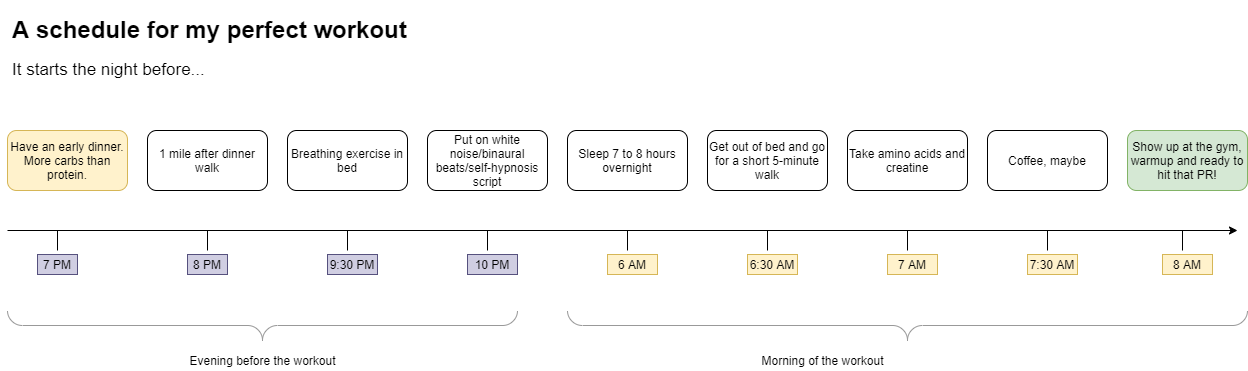
\includegraphics{pictures/routine.drawio.png}
The basic theme in the above workflow is to optimize for a good night sleep (ideally 8 hours) followed by an energized morning hitting the gym with boosted dopamine levels ready for that PR. The following table talks some more about the individual steps in the workflow.

\begin{longtable}[]{@{}
  >{\raggedright\arraybackslash}p{(\columnwidth - 2\tabcolsep) * \real{0.50}}
  >{\raggedright\arraybackslash}p{(\columnwidth - 2\tabcolsep) * \real{0.50}}@{}}
\toprule
\begin{minipage}[b]{\linewidth}\raggedright
\textbf{Step}
\end{minipage} & \begin{minipage}[b]{\linewidth}\raggedright
\textbf{How it helps}
\end{minipage} \\
\midrule
\endhead
Early dinner. More carbs than protein. & Helps sleep through the night. Carbs will raise the blood sugar levels helping to fall asleep and stay asleep. \\
1 mile after dinner walk. & The sights and sounds of the late evening provide visual and audio cues to the brain that it is time to wind down and sleep. \\
Breathing exercise in bed. & Relaxes the body and helps detach the body from any mental stresses we may have experienced during the day. \\
Put on binaural beats/white noise/self-hypnosis script. & Regular pre-sleep ritual to help fall sleep faster, go into deep NREM (non-rapid eye movement) sleep. \\
Sleep 7 to 8 hours overnight. & All the magic happens when we are sleeping. Muscle building, rest and recuperation. \\
Get out of bed and go out for a 5 to 10-minute walk & The sights and sounds of the post sunrise morning time provide visual and audio cues to the brain that it is time be alert and get ready to move around. \\
Take amino acids and creatine & Early mornings pre-workout is arguably the best time to take amino acids for muscle building. \\
Black coffee & Coffee provides the dopamine hit that makes us ready to move and achieve our target. \\
Show up at the gym, warmup and ready to hit the PR & The hardest part yet, showing up! Also, never forget to warmup before doing any heavy lifting to avoid injuries. \\
\bottomrule
\end{longtable}

\hypertarget{best-time-of-day-for-a-workout-for-us}{%
\section{Best time of day for a workout (for us)}\label{best-time-of-day-for-a-workout-for-us}}

While acknowledging that there is not a one size fits all solution (for most things), I would say that there are several advantages for working out first thing in the morning before the start of the workday. Over the past 2 years we experimented with working out in the morning (8am), the afternoon (1pm), late afternoon (4pm) and evenings (6pm). The mornings worked best. Not only did we have more energy before and after the workout but there were several other advantages as I list below.

\begin{enumerate}
\def\labelenumi{\arabic{enumi}.}
\item
  For most people the most difficult part of getting a workout in is getting into a habit of getting the workout in. The more we delay it during the day the more the chances of life events coming in the way and that does not allow the habit to form. Once a morning workout becomes a habit it ceases to become a decision point, it is just something that you do in the morning, same as brushing your teeth.
\item
  A good workout increases focus (thanks to dopamine) and uplifts the mood (thanks to endorphins, the happiness hormone), it is a physiological phenomenon, not just something that we have to imagine. For me personally, workout is part of my workday (at least that is how I like to think about it) at the very least it is a non-negotiable precursor to my workday. Between the hours of 9am to 1pm, I feel super productive because I can think faster and focus better. I now try to front load the more difficult part of my day's work in the first half.
\item
  There is something to be said about the cortisol (the stress hormone) levels and exercise. In the morning the cortisol levels are at their peak due to their natural circadian rhythm so working out during the morning can take advantage of that. The brain signals the adrenal glands to secrete adrenaline, which makes the heart beat faster thereby supplying more oxygen to the muscles, in simple words, it fills us with energy. Conversely working out in the evenings is not such a good idea because cortisol levels are at their lowest and working out would lead to elevated level of cortisol which would interfere with sleep and cause other undesirable effects.
\item
  Finally, a workout in the morning gives you a win, right at the start of the day! When you complete that difficult set, lift that heavy weight off the ground, you are telling yourself I can do hard things and that thought then just does not remain limited to the workout, it extends to everything that you do during the day.
\end{enumerate}

We have had to adjust in our daily schedule in order to accommodate our morning workouts, but it is totally worth it. If you are not sure what time of day works best for your workouts, go ahead and experiment and see what works best for you.

\hypertarget{a-word-about-pain-fatigue-and-delayed-onset-muscle-soreness-doms}{%
\section{A word about pain, fatigue and delayed onset muscle soreness (DOMS)}\label{a-word-about-pain-fatigue-and-delayed-onset-muscle-soreness-doms}}

I have mentioned this earlier in the book that a few hours after I exercised the very first time, I felt an acute pain in my neck which got worse before it got better in about 24 to 48 hours. Thankfully, that was the only time I had to endure that pain and in the almost two years that I have been working out I have not had an exercise related injury. This is primarily because of the watchful eye of our trainer who pays a lot of attention to our form as we perform an exercise and because we listen to our body, in other words we are very clear about *\_not* pushing through the pain. It is important to understand the difference between pain, fatigue and muscle soreness.

If you feel pain during an exercise, you need to stop or go down in weight. The risk of pushing through the pain and consequently causing an injury to a muscle is not worth the false sense of bravado. The intent is not to fight your body but to respect it and be consistent with your workouts so that your form gets better, range of motion improves, and the muscles get stronger over time and thus what seems difficult today becomes easier tomorrow.

During my early months of workout, I would very often wake up the next morning with muscle soreness or what is technically called delayed onset muscle soreness. It was not pain but more like stiffness, it did not prevent me from getting on with my day to day activities (which let's face it were not physically challenging anyway) but it was, for lack of a better word, a nuisance. I started applying Arnica oil on the sore muscles just before sleeping and it helped, but then as I started working out more days a week the ritual got diluted. I used to keep a small bottle of Arnica oil by my bed so that it was easier to remember to apply it, but I was not very regular. Until one day, I realized, I did not need it anymore, I had not been putting the Arnica oil for a few nights and I was fine the next morning, no soreness. What did this mean? Was I getting stronger? Probably. But more importantly I was recovering FASTER. Clearly the emphasis on sleep, nutrition and a proper warmup routine was helping. Often times people consider the (in my opinion) misleading adage of ``no pain, no gain'' or if you do not experience muscle soreness were your workouts even effective, be that as it may, I am happy at not having to experience soreness after every workout. A better indicator that you are making gains from your workout is body measurements.

There is one exercise though that still triggers muscle soreness for me and that is deadlift and a carry, where I pick up a hexbar with weights and carry it 10 to 12 steps up and back. I usually go up to 255 pounds of total weight with the deadlift and carry and it does cause soreness in the back (specifically in the external oblique abdominal muscles) the next morning which goes away as the day progresses and is completely gone in 24 to 36 hours post workout. I am hopeful that in due course as my form improves and recovery is better the post deadlift and carry soreness would also go away. A little bit (define little bit? it is subjective) of muscle soreness should not prevent you from working out and in my experience a good workout helps the muscle soreness go away much faster.

\hypertarget{sleep-sweet-sleep}{%
\section{Sleep, Sweet Sleep!}\label{sleep-sweet-sleep}}

When was the last time you felt like sleeping because you were physically tired? If someone asked me this question last year, I would certainly have to jog my memory. I have a sedentary job and my work does not provide me any natural opportunities to get up and move.

Now however, on days I have a very good workout, by 8-9pm or so I start feeling like dozing off. By the time I get to bed and lay down, the mind, body and soul everything wants to immerse itself in deep sleep to rest and recuperate. The only words that come to mind to describe that feeling are ``sweet sleep''. Doesn't happen very often, but on days that it does, the feeling is hard to miss. A good workout begets good sleep. There is a bi-directional relationship between sleep and workout, a good night sleep makes the workouts the next morning better and a good workout during the day helps get a good sleep at night.

\hypertarget{chapter-5-at-a-glance}{%
\section{Chapter 5: At a glance}\label{chapter-5-at-a-glance}}

\begin{center}\rule{0.5\linewidth}{0.5pt}\end{center}

\begin{enumerate}
\def\labelenumi{\arabic{enumi}.}
\item
  A regular workout routine that focuses on strength training provides \textbf{freedom} from having to count calories and eat foods that we love (in appropriate quantities).
\item
  It is never too late to start working out, I started on the other side of 40. \textbf{The right time to start may have been yesterday, but the best time to start is today.}
\item
  Have aspirational goals but aim for consistency in routine. Getting a set number of workouts in week after week, month after month will set you on a path where the goals are just milestones on a highway and not the focus of your journey, they will take care of themselves.
\item
  This one is personal: for me having the trainer was one of the key reasons why I could stay on track injury free (fingers crossed), motivated and making progress.
\end{enumerate}

\hypertarget{what-did-we-accomplish}{%
\chapter{What did we accomplish?}\label{what-did-we-accomplish}}

I have said this earlier in this book, my initial goal in meeting with a trainer and going to the gym was to lose weight, but as we started sweating it out I realized that we were getting a lot more out of this exercise and clean eating regimen than just a lighter body. Even so, weight loss and overall getting the body in a better shape are important goals, so how did we fare on these?

\captionsetup[table]{labelformat=empty,skip=1pt}
\begin{longtable}{cll}
\caption*{
{\large \textbf{Important Metrics}} \\ 
{\small Key data points that describe the journey}
} \\ 
\toprule
Metric & Amit & Nidhi \\ 
\midrule
Days since start & 600 & 600 \\ 
Days taken to lose last 10 pounds & 48 & 577 \\ 
Starting Weight (lb) & 251.33 & 151.9 \\ 
Current Weight (lb) & 183.87 & 133.82 \\ 
Total weight loss (lb) & 67.46\textsuperscript{1} & 18.08\textsuperscript{2} \\ 
Best Weight loss month & May, 11.91 lb & Oct, 9.26 lb \\ 
 \bottomrule
\end{longtable}
\vspace{-5mm}
\begin{minipage}{\linewidth}
\textsuperscript{1}26.84\% of the starting body weight. \\ 
\textsuperscript{2}11.9\% of the starting body weight. \\ 
\end{minipage}
\begin{minipage}{\linewidth}
Source: Daily measurements done @home\\ 
\end{minipage}

I would be remiss if I do not mention that men and women respond to exercise and diet differently. While it is true that I had a lot of weight to lose as compared to Nidhi, but it is also true that she was losing weight at a much slower pace and had several phases where her weight loss just stalled. Both of us did the same workouts (for the most part) and ate pretty much the same food, but I could lose weight and she found it very hard. Important to have realistic expectations and continuously work with your trainer to evaluate what could be tweaked.

\hypertarget{percentages-are-revealing}{%
\section{Percentages are revealing}\label{percentages-are-revealing}}

I reached my weight goal of 190lb in in early 2021 and then decided to go even lighter so that I weight between 180lb to 185lb. I am no longer obese, although technically overweight. However, I am much lighter and much stronger at 42 years of age than I felt at 22 years. I bet 22-year-old me would not be able to run a mile without gasping for air, more like not able to run a mile at all, period. I have a target of being able to deadlift 400lb and so I intend to stay around 185lb and not lose any more weight. Once you understand how your body responds to certain foods and cut out refined sugar from your diet, losing weight becomes straight forward unless you have other issues.

So, net-net in about 22 months, I lost about 27\% of my body weight and Nidhi lost about 12\%. Not too bad. In terms of how far we have progressed compared to the goals we started with, well the goals are just milestones along the way, the journey continues.

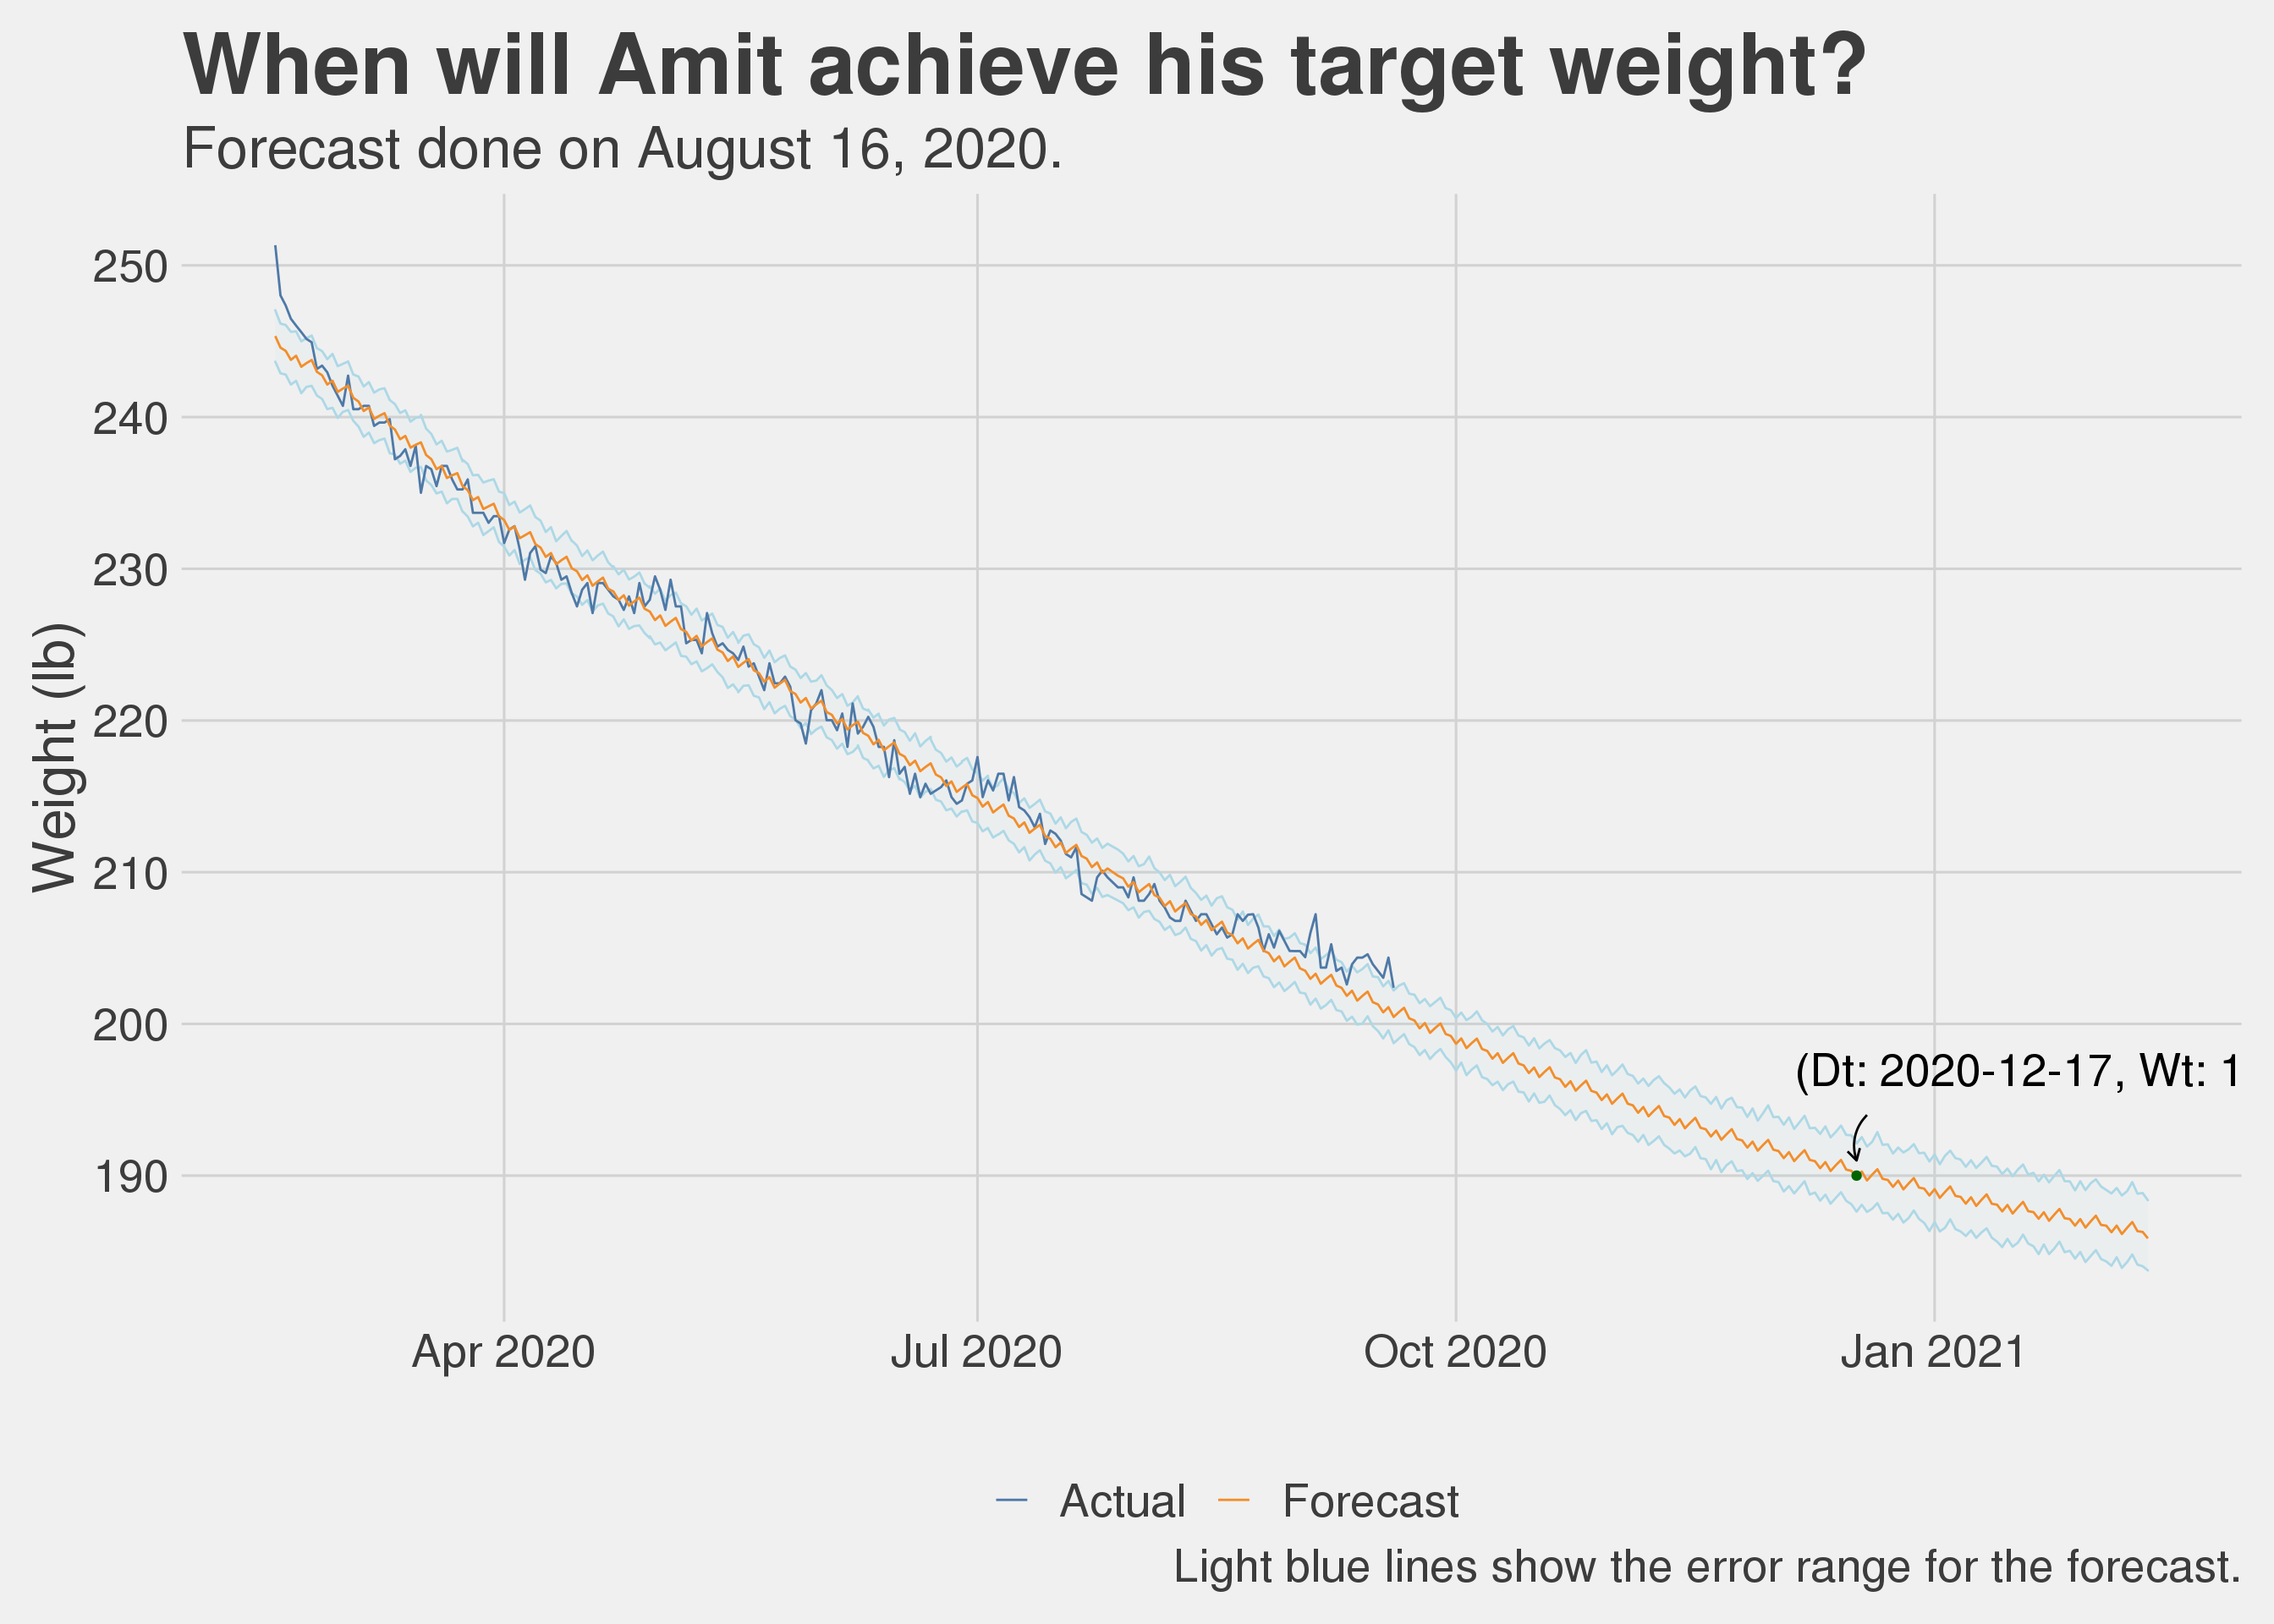
\includegraphics{bookdownproj_files/figure-latex/unnamed-chunk-17-1.pdf}

\hypertarget{changes-in-other-biometrics}{%
\section{Changes in other biometrics}\label{changes-in-other-biometrics}}

Along with the body weight, other metrics also saw significant change. This is seen in the following charts. BMI is widely used (I suppose accepted as well) measurement to determine if someone is healthy, obese or overweight. We saw reduction in BMI as well which as expected is correlated to the reduction in weight. NIH guidelines for BMI are available \href{https://www.nhlbi.nih.gov/health/educational/healthdisp/pdf/tipsheets/Are-You-at-a-Healthy-Weight.pdf}{here} for reference.

All measurements in the charts below were done automatically as part of the daily metrics measured by the scale and synched with our phone. This made it easy to collect and analyze this data.

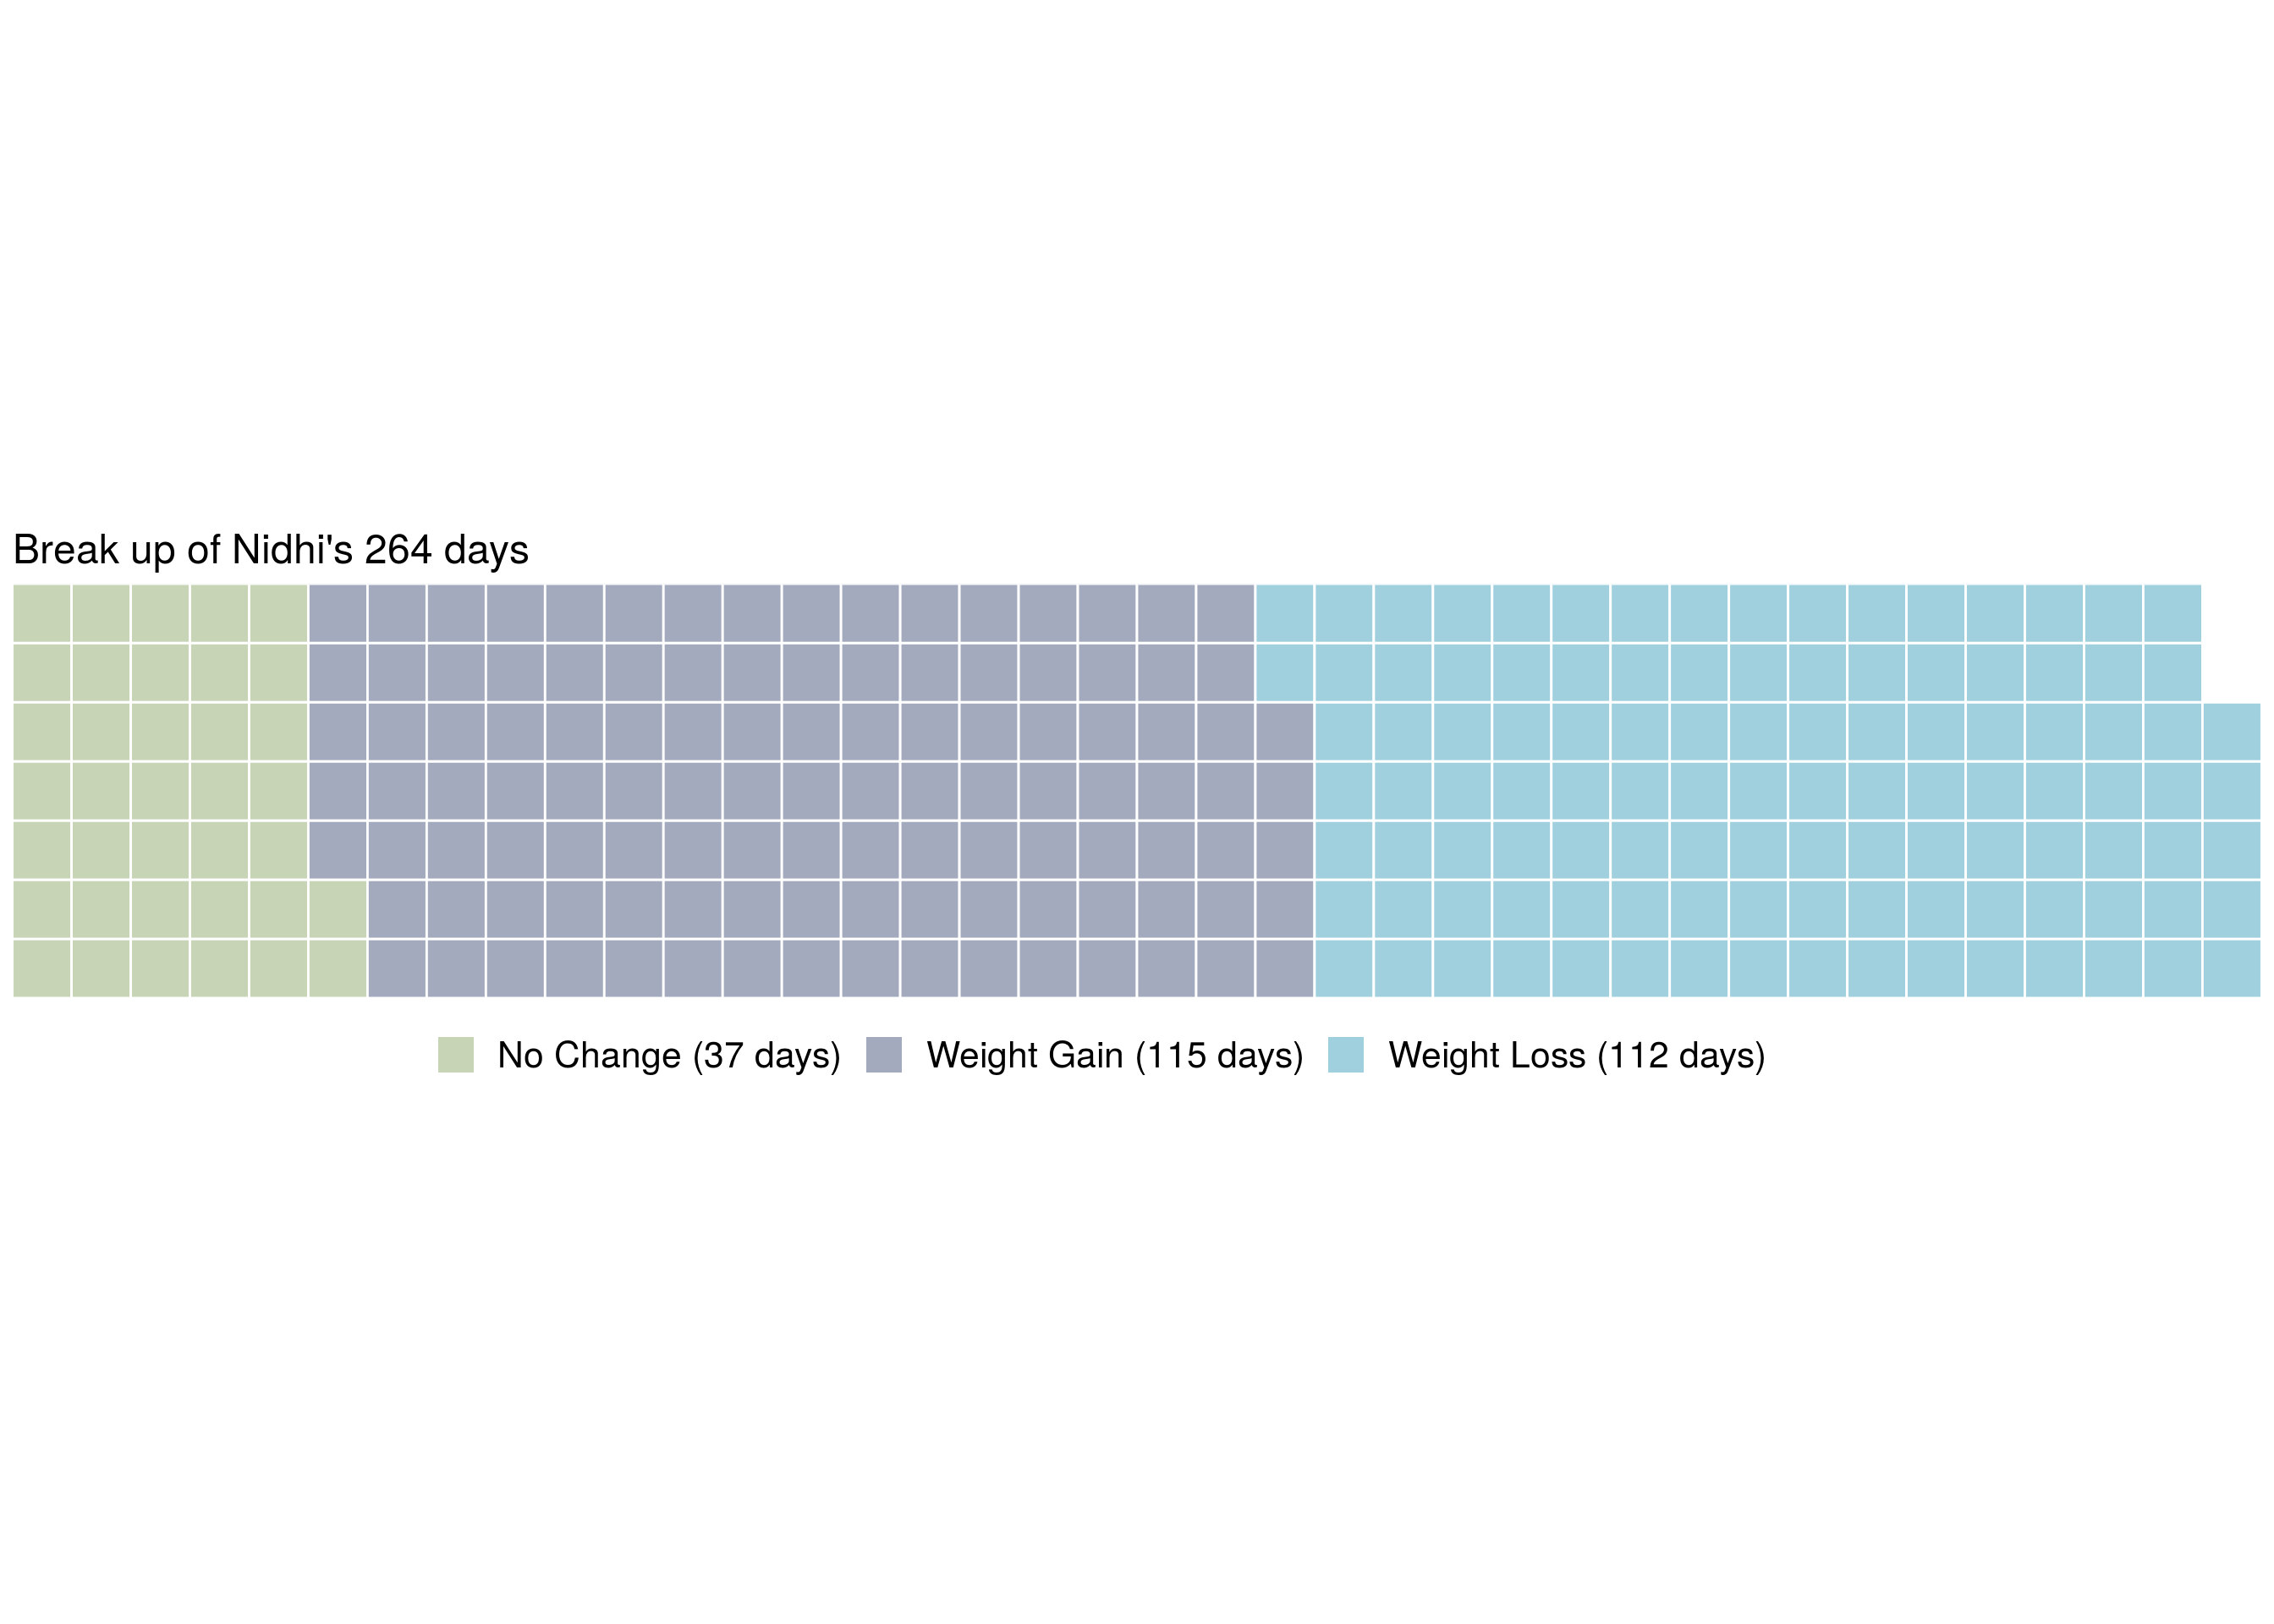
\includegraphics{bookdownproj_files/figure-latex/unnamed-chunk-18-1.pdf}

\hypertarget{body-measurements}{%
\section{Body measurements}\label{body-measurements}}

Weight and BMI is not the only metric we tracked; these metrics are often times all we think in terms of measuring but there is more. Just as the proof of the pudding is in the eating, the proof of the weight loss is in the wearing (of clothes). As we kept on making progress in our journey, the clothes started fitting well at first, then getting loose and the finally it reached a point where most of our old clothes were just too big and this necessitated a wardrobe refresh. A happy problem to have.

We tracked this by doing body measurements once every few months. The charts below have a story to tell.

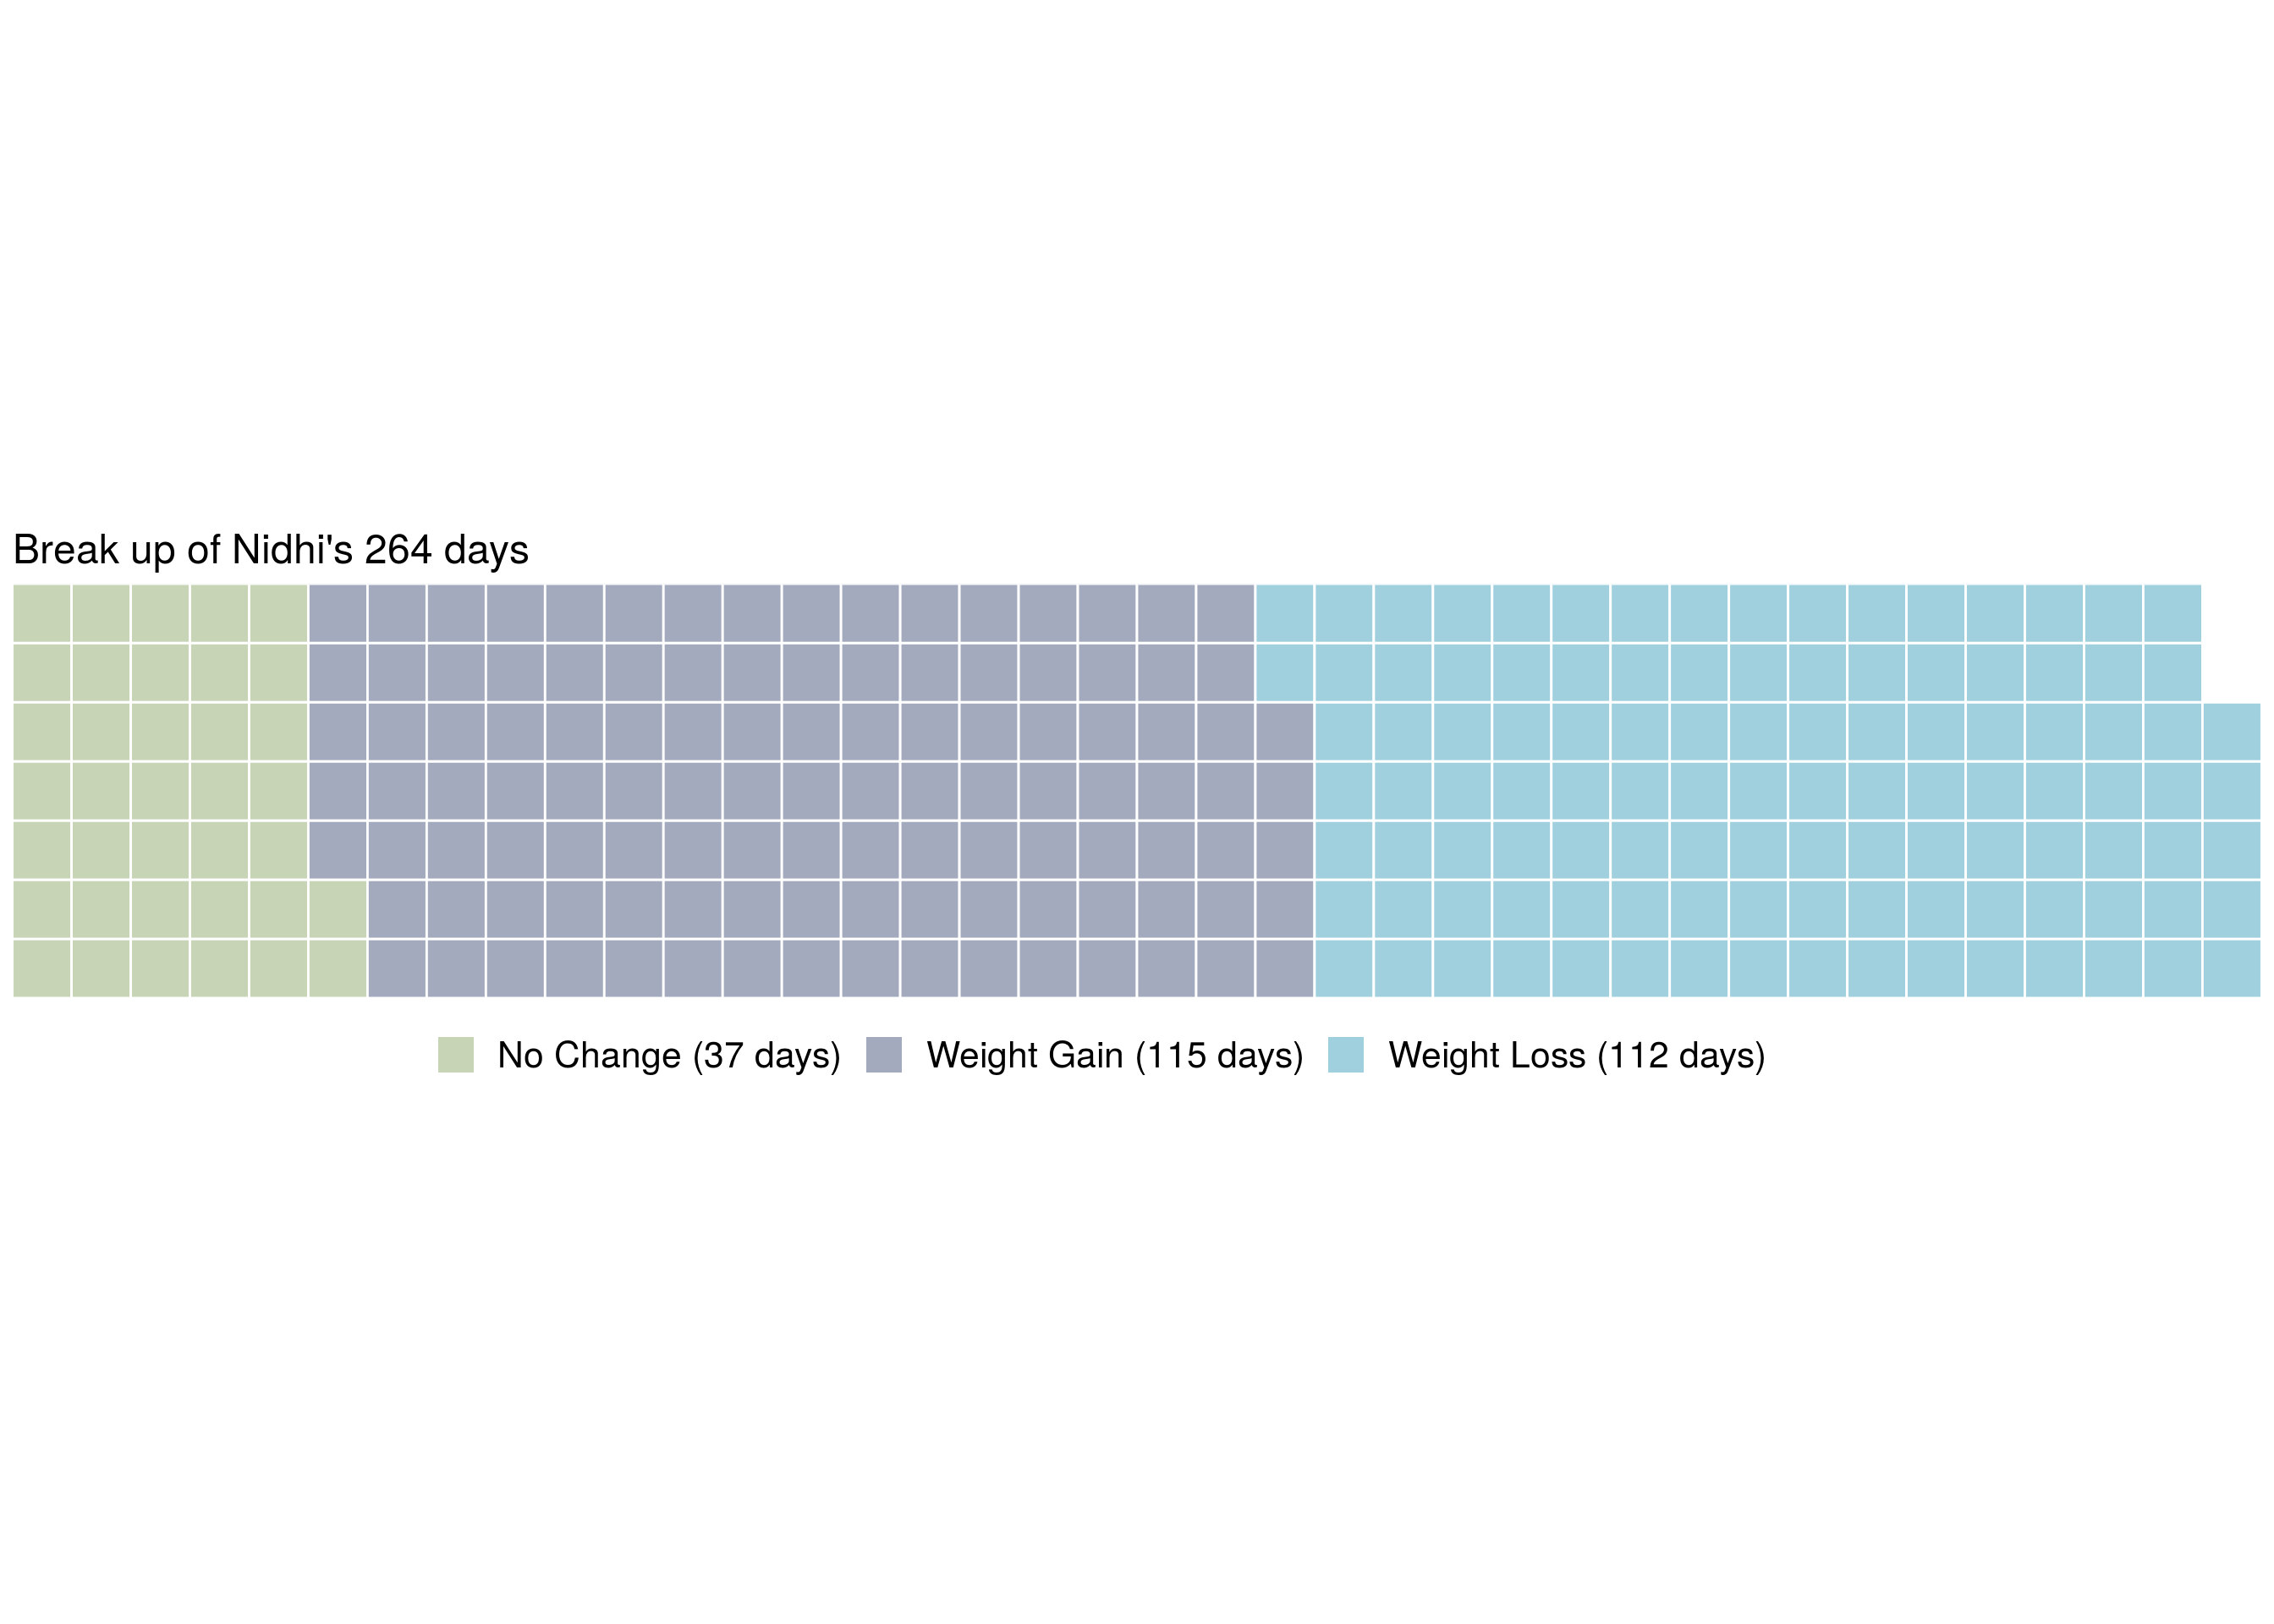
\includegraphics{bookdownproj_files/figure-latex/unnamed-chunk-19-1.pdf}

\hypertarget{of-slides-and-plateaus}{%
\section{Of slides and plateaus}\label{of-slides-and-plateaus}}

Anyone who has embarked on a journey to lose more than say 10 pounds would identify with the fact that the weight loss trajectory is never a linear slide downwards, no matter how determined you are in your desire and dogged in your persuasion. It was the same for us, there were days and weeks which were very good, especially at the start and then there were periods where the weight loss yo-yoed. These periods were disappointing, disheartening even.

It is important to understand, as we discovered, that as we are subjecting the body to a different sort of eating regimen and making more and more demands of it by way of workouts in the gym, the body is also trying to recalibrate its response. It is figuring out how much fat to store as energy reserves, how much to burn to provide the fuel for the exercise. This means that sometimes the weight loss may completely stall or even go in the reverse. The key is to be patient and keep eating clean (relatively speaking) and putting in the hours in the gym without completely burning out.

The next chart shows the week by week distribution of the weight and as you can see there were at least a couple of streaks of plateaued weight loss. We persisted, and ultimately, we prevailed.


\includegraphics{bookdownproj_files/figure-latex/unnamed-chunk-20-1.pdf}

\hypertarget{a-forecast-and-a-promise}{%
\section{A forecast and a promise}\label{a-forecast-and-a-promise}}

As we were going through this journey, I was very eager to apply some forecasting and determine if we could project a reasonable date when we would be able to meet our weight loss target. As much as this book is not just about weight loss, there is no denying the fact that it was one of the most (if not the most) tangible outcome we were tracking towards.

\textbf{\emph{NOTE:}} I did this forecast in August of 2020 and tracked it till December 2020. Forecasting weight loss is a complex mathematical problem because it depends upon a multiplicity of (changing) features. I did achieve my target in early 2021 but kept these charts as is as a reminder of where we started and what I was thinking as being possible a few months into the journey.

Once we had collected a reasonable amount of data, I used standard timeseries forecasting techniques to determine how our weights would look say 30, 90 or 180 days from the current date. I used the \href{https://facebook.github.io/prophet/\#:~:text=Prophet\%20is\%20a\%20procedure\%20for,daily\%20seasonality\%2C\%20plus\%20holiday\%20effects.\&text=Prophet\%20is\%20robust\%20to\%20missing,and\%20typically\%20handles\%20outliers\%20well.}{Prophet} package from Facebook AI Research (\href{https://github.com/facebookresearch}{FAIR}) to do the timeseries forecast. The results are presented below. This forecast was done on August 16, 2020 and as per this forecast we should be able to achieve our target weight (128 lb) in early October for Nidhi and mid-December for me (190 lb).

Once we had these forecasted dates and the plots created, we started monitoring very closely if our daily weight measurements were within the range of errors as shown in these plots. Some days the weight did creep out of the error limits but then it served as a nice tool to keep us honest, so in a manner of speaking we knew how much we could deviate. So, if an Indian takeout dinner one evening did set us back, we knew we had to make up for it in the next few days to come back within acceptable range. So far it seems the projects are holding up reasonably well. If nothing else, it provides certain guard rails to not let one go completely off track. The promise still is, if we keep doing what we have been diligently doing, we should be able to achieve our goals around, if not exactly on, the forecasted date. It is important to mention here that this simple forecast is considering the weight loss as a single variable timeseries, we know it is much more complicated than that. There are a lot of factors that would go into making a much more accurate weight loss forecast (if I could do that then maybe I would be writing a different book :)). This is just a simple attempt.

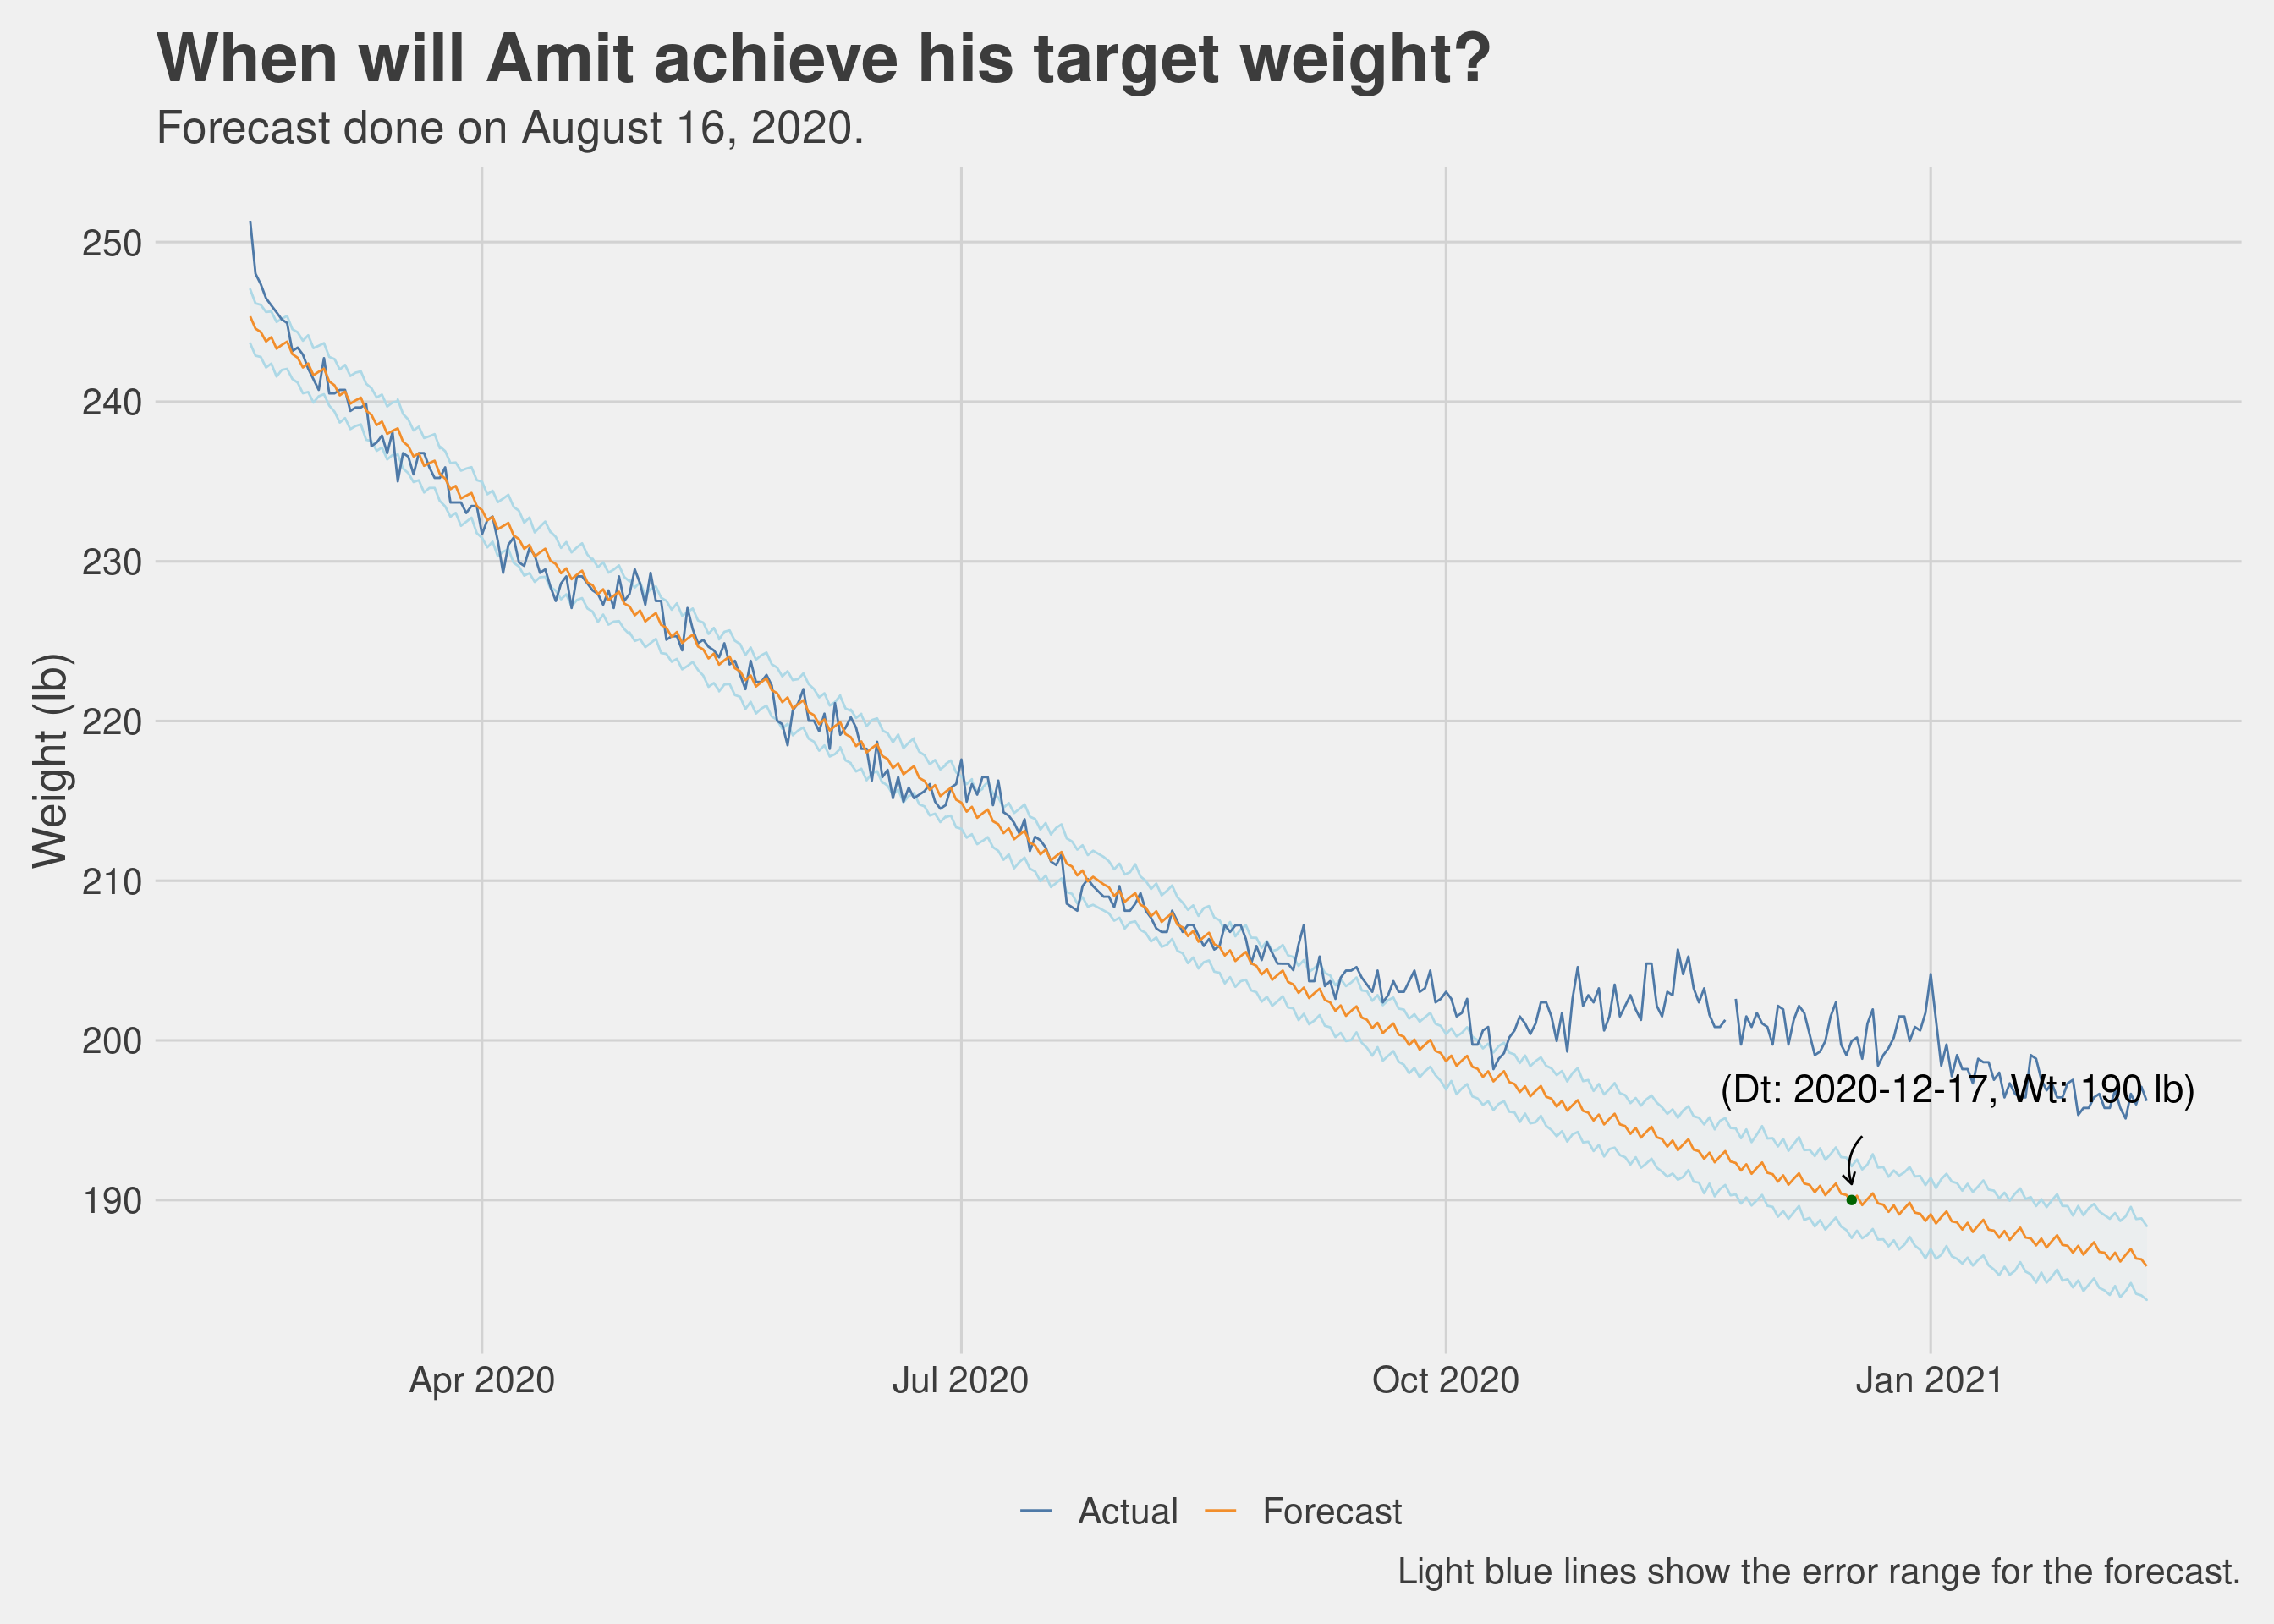
\includegraphics{bookdownproj_files/figure-latex/unnamed-chunk-21-1.pdf}

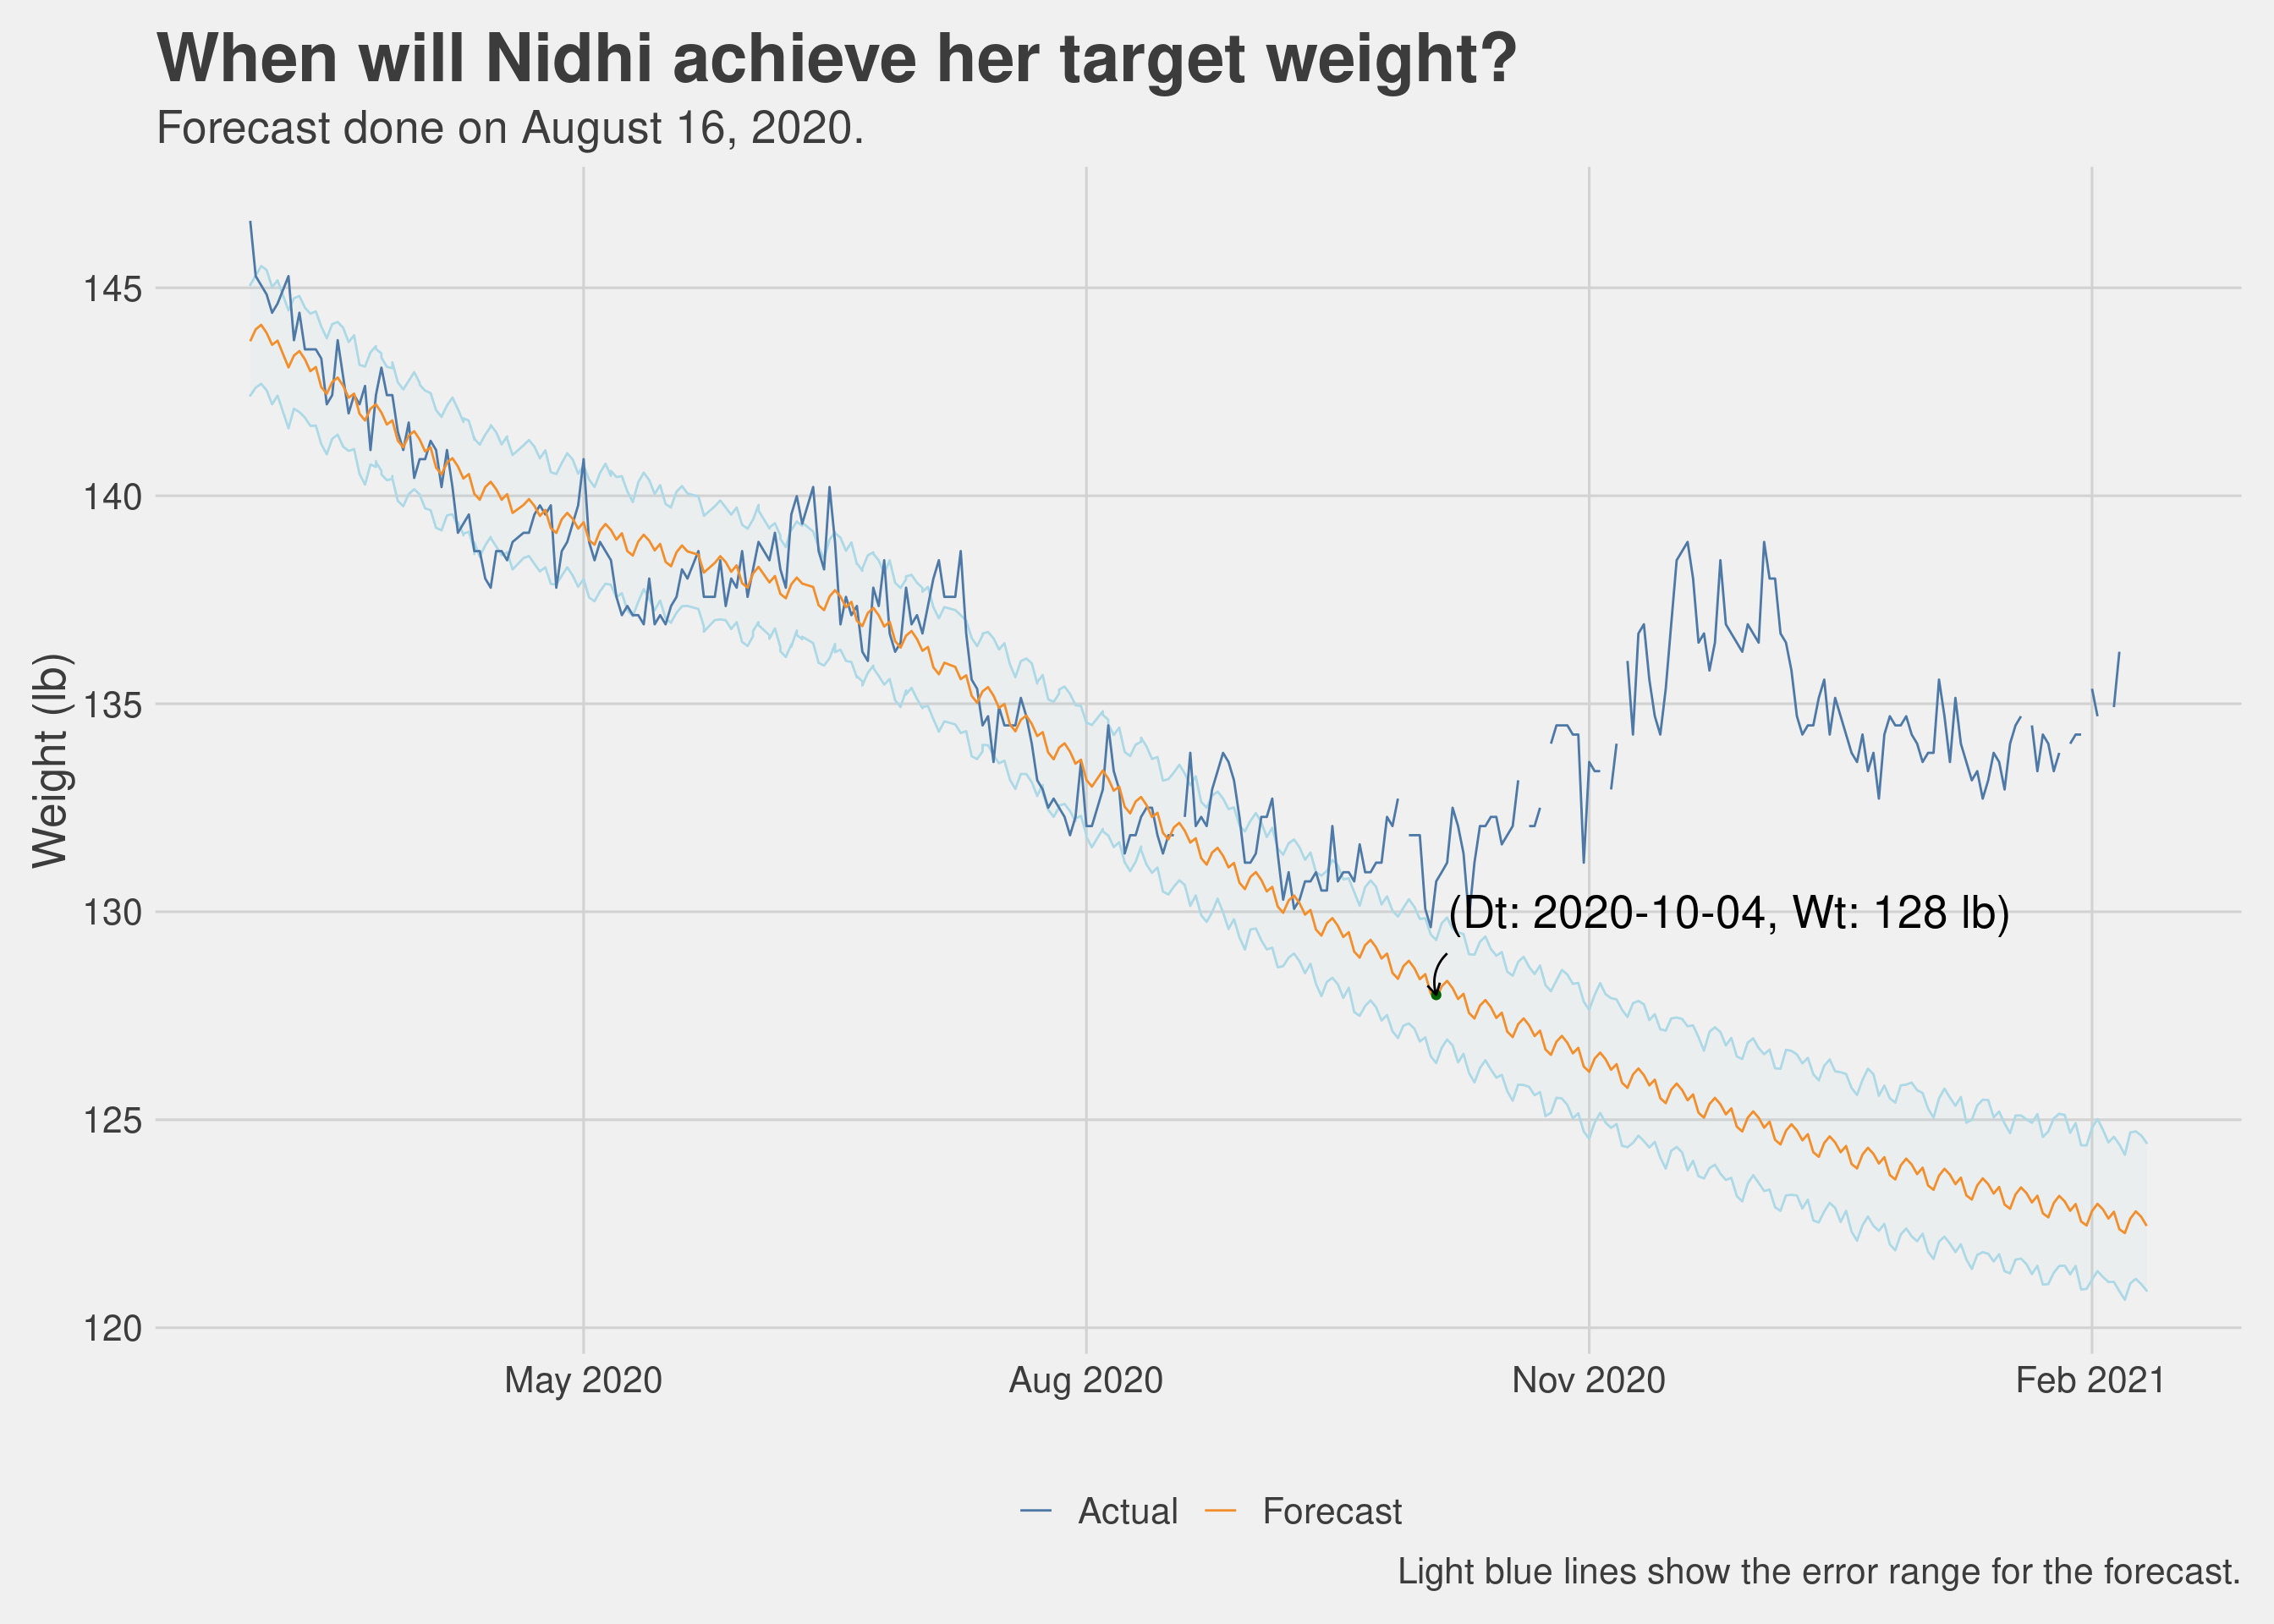
\includegraphics{bookdownproj_files/figure-latex/unnamed-chunk-22-1.pdf}

\hypertarget{losing-weight-is-one-thing-but-keeping-it-off}{%
\section{Losing weight is one thing but keeping it off\ldots{}}\label{losing-weight-is-one-thing-but-keeping-it-off}}

Anybody who has ever lost any amount of weight, even if it is 5 pounds (or some would say especially if it is 5 pounds) would tell you that it always comes back. Well, how did we fare in that regards?

The chart below shows my daily body weight since the start of 2020. I was able to reach my target body weight of 190lb and have been able to maintain between 185lb to 190lb since then (7 months as of this writing). No mean feat for someone who had never been fit before and the good part is that I have been able to do it not by tapping into some deep hidden reserves of will power but all while leading what I would consider a \textbf{normal} lifestyle that involves vacations, eating out every now and then and having a decent social life. In other words, it did not involve living in a cave or carrying my own food with me everywhere.

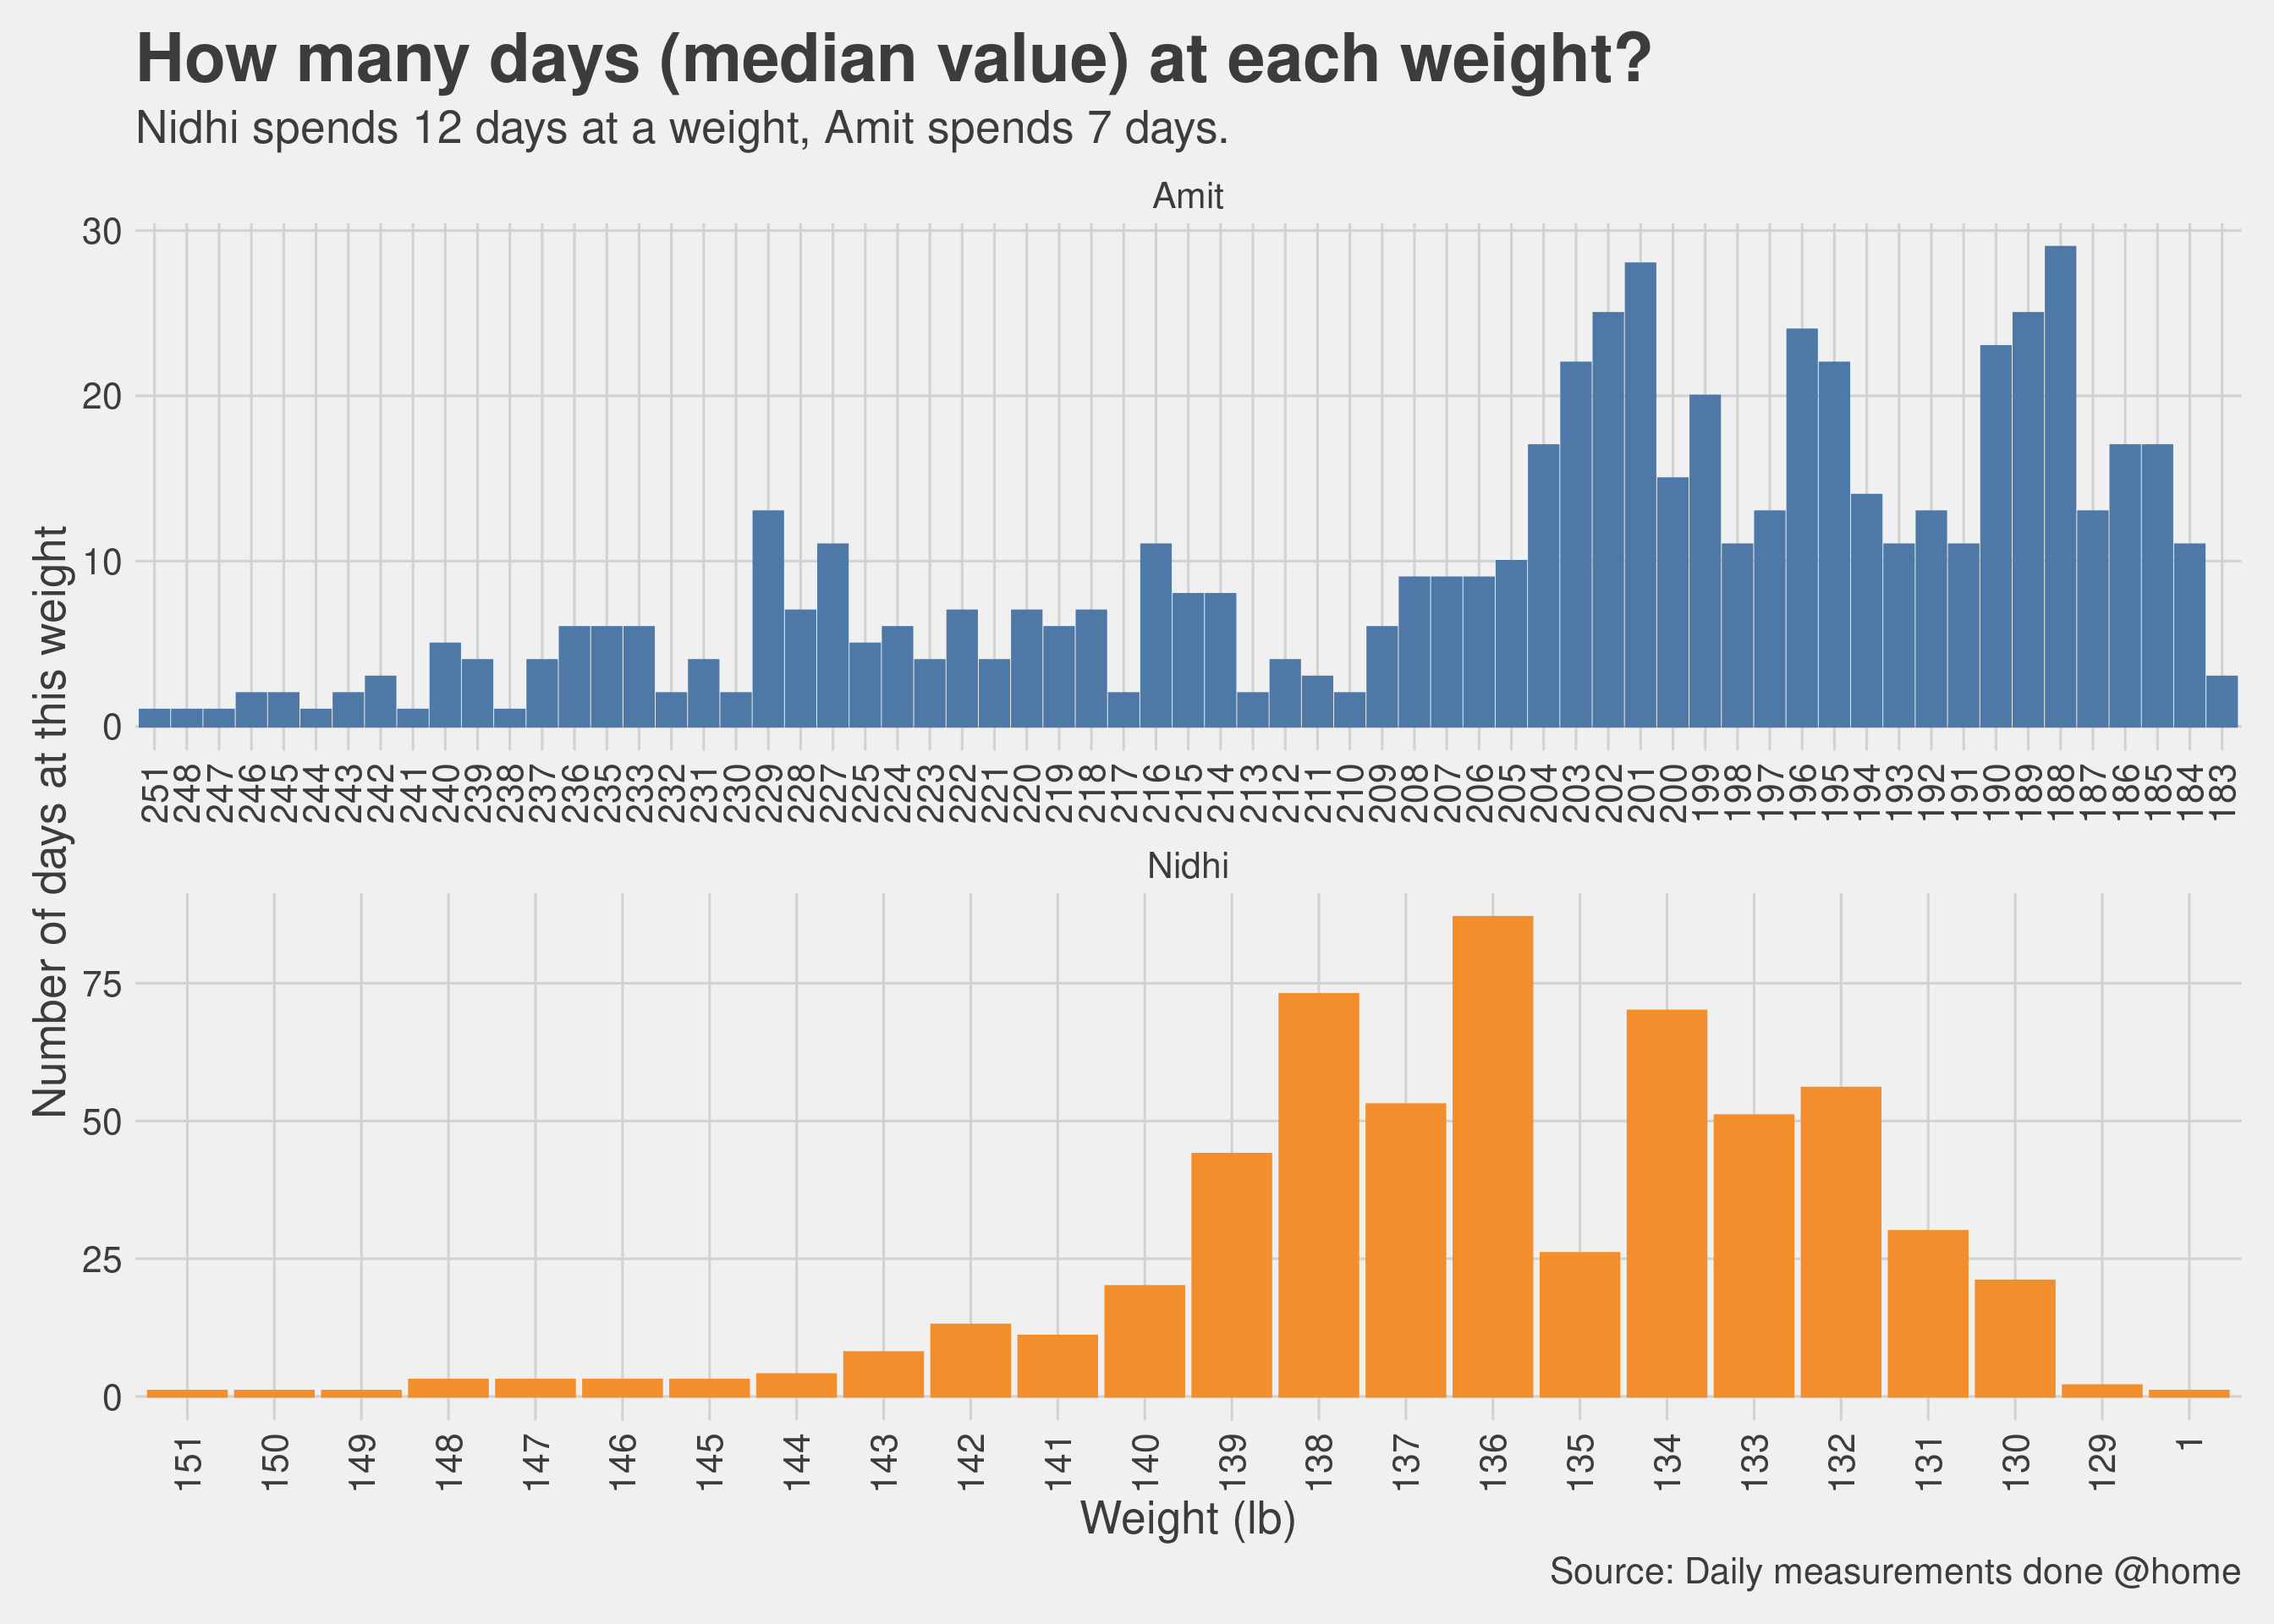
\includegraphics{bookdownproj_files/figure-latex/unnamed-chunk-23-1.pdf}

So, here is the secret recipe that works for me. As you can see there is hardly any noble prize-winning research here, just \textbf{simple things, \textbf{done} \textbf{consistently}}.

\begin{longtable}[]{@{}
  >{\raggedright\arraybackslash}p{(\columnwidth - 6\tabcolsep) * \real{0.25}}
  >{\raggedright\arraybackslash}p{(\columnwidth - 6\tabcolsep) * \real{0.25}}
  >{\raggedright\arraybackslash}p{(\columnwidth - 6\tabcolsep) * \real{0.25}}
  >{\raggedright\arraybackslash}p{(\columnwidth - 6\tabcolsep) * \real{0.25}}@{}}
\toprule
\begin{minipage}[b]{\linewidth}\raggedright
How strict I am about this?
\end{minipage} & \begin{minipage}[b]{\linewidth}\raggedright
Category
\end{minipage} & \begin{minipage}[b]{\linewidth}\raggedright
Activity
\end{minipage} & \begin{minipage}[b]{\linewidth}\raggedright
How well did I really stick to this?
\end{minipage} \\
\midrule
\endhead
Non-negotiable & Food & Absolutely no soft drinks (soda) and barely any hard drinks. & Yes, for the most part. My alcohol consumption is practically zero now, had a few drinks during the holidays though, have not had a soda for about 2 years now. \\
Non-negotiable & Food & No dairy products (except homemade curd and cottage cheese, occasionally). & Yes, for the most part. Made an exception for some homemade Indian sweets during the festival season. \\
Non-negotiable & Food & No cakes, pastries, canolies, muffins or bread. & Yes, for the most part. Goes without saying that I did have cake on my kids' birthdays and our wedding anniversary. \\
Non-negotiable & Food & Don't want to name names but you won't find me dead in a fast food restaurant chain. & Yes, no exceptions, even when we were on long road trips. \\
Non-negotiable & Food & No caffeine after 3pm & Yes, for the most part. \\
Non-negotiable & Food & Warm water or no-caffeine/herbal tea 30 minutes after dinner. & Yes, for the most part. \\
Non-negotiable & Workout & 5 days of strength training with an occasional 6th day of light cardio such as long walks. & Yes, no exceptions, even when we went on vacations, I worked out in the hotel's fitness center. \\
Best Effort & Eating Habits & A 16-8 or at least 14-10 eating window. & Yes, no exceptions, even when we went on vacations. \\
Best Effort & Eating Habits & Eat most of my protein and fiber in the first half of the day and most of my carbs during dinner (preferably 7.30pm, no later than 8pm). & I try hard, but of course, I fall short sometimes. \\
Best Effort & Eating Habits & 2 to 3 days of water fasting every month. & This is a hard goal (although not as hard as it might seem at first glance) but we were able to do it consistently for most of 2021. \\
Best Effort & Lifestyle & Short morning walk, 1 mile after dinner walk & Recent addition to my routine, able to do it at least 4 times a week. \\
Trying to improve & Sleeping Habits & While the goal is 8 hours, I manage just about 7 hours on most days. This is a stretch goal and something I need to work on. & Not so good. \\
Trying to improve & Lifestyle & Breathwork practice, for sleep, relaxation and workouts. & Working on it. \\
Trying to improve & Lifestyle & Read more books, very selective engagement with social media. Why is this important? Because, there is no physical health without mental health and vice-versa. & Working on it. \\
\bottomrule
\end{longtable}

So, I cannot end this chapter without mentioning about Nidhi's journey, did she achieve her target. Well, if we go by numbers, she isn't 130 lb today, for most of 2021 her weight has been between 133 lb and 138 lb. There were setbacks in terms of her getting Covid, and some other health issues, but she bounced back and is constantly marching towards her goal. Due to regular workouts, even at 135 lb she looks (and indeed is) fitter than a year ago because her body structure has become toned and athletic. To my mind, she is perfect the way she is.

\hypertarget{chapter-6-at-a-glance}{%
\section{Chapter 6: At a glance}\label{chapter-6-at-a-glance}}

\begin{center}\rule{0.5\linewidth}{0.5pt}\end{center}

\begin{enumerate}
\def\labelenumi{\arabic{enumi}.}
\item
  Regular body weight measurements and other biometrics along with body measurements were very helpful in keeping us on track during our weight loss journey and beyond.
\item
  Life happens and that will provide an occasional pause in the weight loss journey, and that is OK if we get back on track right away. Social dinners, going on trips, making exceptions for a late evening ice-cream after dinner is all par for the course.
\item
  Losing weight and keeping it off are two different problems and should be approached as such. Weight loss can be accomplished by intensity (generally people can stick to a diet, any diet, for a few months maybe, especially when they start seeing results), but keeping the weight off requires consistency. It ultimately comes down to a binary choice ``healthy and therefore happy in the long term OR consciously unhealthy right now for sort term pleasure but miserable tomorrow and beyond''. I know its a harsh statement but it really is a question we need to ask of ourselves and it's answer will inform us of why we are the way we are.
\end{enumerate}

\hypertarget{our-diet-now}{%
\chapter{Our Diet Now}\label{our-diet-now}}

Towards the end of 2020, we had an outdoor get together with some very close friends and as we were sitting around the fire pit chatting and laughing one of our friends said ``bring the brinjals, lets grill them so that you can make a \href{https://en.wikipedia.org/wiki/Baingan_bharta}{baingan ka bharta} tomorrow!''. the ``Baingan ka bharta'' is a delicacy made with grilled minced eggplant. So, we got two brinjals, they were grilled and the next day we did make the ``bharta'', ate it with crisp tawa rotis and green chillies. It tasted divine. The reason I mention this is that after about 8 months of eating what was essentially a high protein, high fiber and low carb diet, we were slowly but surely wanting to get back to traditional food that we had eaten most of our adult lives and our parents and grandparents had eaten most of their lives. Eating the bharta that day reminded us that we missed our traditional Indian food more than we realized.

As more months went by, roti, rice, pulses cooked in a pressure cooker and cooked vegetable curries became more and more a part of our dinners like they had always been. We still love our grilled veggies and chicken though and eat it multiple times a week. The lunch for us is still one of our favorite salads on most days. The breakfast, however, is what is the most different because the ``lunch'' is the ``breakfast''. Allow me to explain.

\hypertarget{the-breakfast-that-isnt}{%
\section{The breakfast that isn't}\label{the-breakfast-that-isnt}}

When we started training, and our trainer mentioned the 30-day challenge, she also mentioned something that we simply ignored (one of the rare things that she said and I just forgot). It was that she did not eat breakfast or said another way her first meal of the day with which she broke her overnight fast (break-fast) was lunch.

It did not even occur to me that it was something to consider, I did not pay much attention to it at all. As I became more interested in nutrition and ageing and longevity, I started hearing more and more about intermittent fasting. There are two schools of thought, one that says you should keep eating small meals multiple times a day and another one which says you should eat two or three full meals a day and no snacks. I can only speak from what I experienced, eating full meals and no snacks works best for us. Just to state it again, \emph{whatever I am writing here is not medical advice, please consult your doctor before starting any new diet or exercise and confirm that it is appropriate for your specific situation and life circumstance. Children should not skip breakfast; my kids eat a healthy breakfast early in the morning}.

By intermittent fasting, I mean a 12 hour fast and a 12-hour eating window OR a 14 hour fast and a 10-hour eating window OR a 16 hour fast and an 8-hour eating window. Depriving oneself of any and all foods that one likes during the week and then gorging on all sorts of unhealthy foods over the weekend is not my idea of intermittent fasting. I started with a 12-12 fasting and eating window and have now comfortably settled into a steady 16 hour fasting and 8 hour eating window and it works great for my body and mind. I prefer intermittent fasting over the eating 6 meals a day routine for several reasons that I list below.

\begin{itemize}
\item
  Eating clean and healthy 3 times a day is difficult as is in a modern city based lifestyle, eating clean and healthy 6 times a day is almost impossible unless you are an athlete or a movie star and have someone on your staff whose job is to take care of your nutrition. I just don't trust myself to make the correct choice for food 6 times a day, every day.
\item
  All weight loss is ultimately a game of keeping the insulin levels in your blood within a narrow range. Eating multiple times a day means blood sugar levels will increase in response to the carbs being broken down into glucose and that means the pancreas will produce insulin.
\item
  I feel bad while writing this, but I cannot deny that not having to prepare and eat breakfast is a decent 30 minutes of time saved at the start of the day. While this should not be a factor, but the reality is that it is. I like to use those 30 minutes for my morning walk, for reading a book and sometimes for replying to some quick work-related emails.
\end{itemize}

All my adult life I had eaten three full meals a day, the idea that there is no breakfast was so much out there that even until a few months ago I used to think that if you do not eat breakfast how do you even function! Not anymore. I feel fantastic with my 16-8 routine. I realized that often times when due to some work related crisis in the morning I could not eat breakfast until noon, my brain actually worked much better, now it could simply be a result of being very focused on the problem but it was definitely something I considered when trying intermittent fasting.

While I do not eat breakfast, but I do take my morning coffee (no cream or sugar), sometimes with 10 to 15ml of MCT oil added to it to make it the so-called \textbf{Bulletproof Coffee}. The MCT oil provides the fat which they say gives you energy, clears brain fog and has other benefits. I am not so sold on the benefits; I do take it every now and then. Recently though, instead of the morning coffee I have started taking microgreens, available as powder that you can just mix in cold water and drink and then take my coffee an hour or so later at the start of my workday. This arrangement works much better for me. The microgreens help provide several essential pre and postbiotics, vitamins and minerals. I have seen several nutritionists recommending not to take coffee right after walking up. Drinking coffee on an empty stomach could cause gut health issue, change the Cortisol production cycle, so I am happy that have shifted my coffee intake to about two hours (or sometimes even more) after waking up. While on the topic of caffeine, I don't drink coffee after 3pm and rarely, if ever, after 4pm. Here is a picture of the microgreens drink, first thing in the morning.

\begin{figure}
\centering
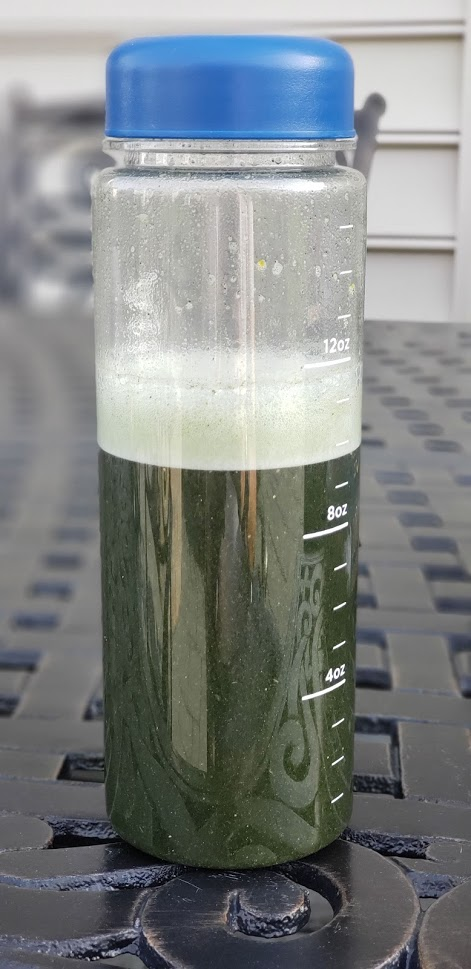
\includegraphics{pictures/microgreens.jpg}
\caption{Microgreens}
\end{figure}

\hypertarget{the-lunch}{%
\section{The lunch}\label{the-lunch}}

One thing that has relatively stayed the same, and which also explains the unchanged name of this book, is the lunch salad, of course with blueberries. It is still something we greatly enjoy eating. The fact that it is something that is healthy and tastes good means that there isn't any need to change it. I mean why fix something that is not broken? Our lunch is usually around 1pm.

The salad still consists of a healthy dose of cruciferous vegetables such as a kale, broccoli sprouts, cabbage, arugula, brussels sprouts. The benefits cruciferous vegetables are well documented in terms of their antioxidant and anti-inflammatory effects. These vegetables are also good source of fiber and vitamins. There is some research that show that cruciferous vegetables decrease inflammation and reduce the risk of cancer.

We have had two additions to our salad: Broccoli sprouts and Hemp seeds. I learnt about the benefits of broccoli sprouts in a Podcast that I listen to and when I saw them in a local supermarket, I immediately decided to try them out. So now our salads often contain a few grams of Broccoli sprouts (they have a very small (fridge) shelf life). These wonderful sprouts contain glucoraphanin which our bodies convert into a compound called sulforaphane that helps in fighting cancers, ulcers and even supposed to have mental health benefits. Hemp seeds are a great source of plant-based protein, essential fatty acids and some vitamins and minerals. We use it off and on in our salads. More discerning readers would know that hemp seeds contain trace amounts of THC (\textless{} 0.3\%), the active compound in marijuana. I suppose the jury is still out on the inclusion of hemp seeds into functional foods.

There is a growing interest in using plant based chemical compounds for improving cellular defense mechanism and we just feel happy about making the good choices wherever we can.

Eating salads, so consistently has been a very distinct shift from our eating habits growing up. While we always were aware of the idea that eating raw uncooked vegetables is beneficial but then how much of raw vegetables could you consume. Growing up, my lunch used to have cucumber, radish, cabbage and onion as salad but it was an adjunct and that too not every day and slowly as I went for higher studies, entered professional life, the amount of raw uncooked vegetables I consciously consumed just kept on reducing. Whereas now, a hearty salad, rich in fiber, proteins and good fats, that completely fills us up \emph{is our lunch} at least five days a week. The lunch salad is probably the most fundamental and probably the most beneficial change in our diet. Nowadays, if I eat a heavy lunch such as a high carb lunch at a restaurant or sometimes even at home then within an hour or so of eating the lunch the familiar old feeling heaviness, lethargy and sleepiness returns. I am now so used to maintaining constant energy levels through the day that feeling sleepy in the middle of the day, is just, terrible. Sometimes when meeting friends or at social events people give me the reaction that ``oh, you are doing such a great job of watching what you eat, what a sacrifice to make for good health!'' and I must explain to them ``actually, no, it is not at a sacrifice at all, what it is that now I don't want to trade 3 hours of feeling sub-optimal for 20 minutes of taste, that is all\ldots{}''. This body is not a loaner!

Well, as it turns out, the salad is not the end of our lunch. To top it off, I usually take a protein bar (we choose one of the bars that has minimal ingredients) or sometimes a spoonful of Moringa powder with water after the salad. It does not taste good, but boy is it beneficial! \emph{Moringa Olifera} is a widely grow in Asia and Africa and is native to North Western India, the exact part of the Indian subcontinent from where my grandparents came. It is interesting that when I was describing Moringa to my mother, she mentioned to me that my grandfather used to get that plant often as a vegetable to be had as part of lunch. Moringa is called \emph{Sehjan} in Hindi. It has several documented health benefits such as being good for digestion, helps with medical conditions such as high blood pressure, diabetes, obesity etc. But the one health benefit that I noticed right from the first day was that it helps keeps my insulin levels constant and energy levels up. Now, I do not have a continuous glucose monitor (CGM), not yet anyway, to be able to prove it with data but I certainly think that is the case.

On days when I don't have Moringa powder after lunch, I take a black coffee along with my protein bar. This is my last cup of coffee for the day.

\hypertarget{the-4pm-snack-1}{%
\section{The 4pm snack}\label{the-4pm-snack-1}}

As you might have guessed, I no longer feel the need for it. The fiber, proteins and good fats from the lunch keep me full. I do take a caffeine free tea anytime between 3.30pm to 5pm. Sipping a hot beverage helps me focus better, although the documented benefits of sipping hot water (I would like to consider the caffeine free tea to just be flavored hot water) are that helps with digestion, triggers the endocrine system, even helps the muscles relax, but I will go with ``it helps me focus better post lunch''.

\hypertarget{dinner}{%
\section{Dinner}\label{dinner}}

I get back home from work around 6.30pm (I started going back to work soon after I got my second Covid vaccine shot) and at that time I am hungry. I will admit, that before dinner I do end up snacking, could be a few apricots, a couple of figs or very occasionally a slice of frozen grain bread (toasted before eating) with kerrygold butter. This is not ideal, but then, it is better than eating unhealthy snacks.

Ideally, I would like the dinner to be between 7 - 7:30pm but it is more like 7:30 - 8:30pm. We need to pull it back. The dinner has changed since last year. The high protein grilled stuff that we had been eating is now mostly replaced with a conventional North Indian dinner which includes carbs, fat and some protein (in that order). Until a few months ago when I was still shy of my weight target, I used to be very careful about avoiding carbs, but no more. My weight has been stable between 185lb to 190lb for several months now, and that has been with a dinner that contains carb in the form of \emph{Rotis} and cooked vegetables, fats in the form of \emph{Ghee} and proteins either from chicken or fish or pulses.

It was in February 2021, almost one year after we switched to a high protein low carb diet, that I started noticing that I could not sleep through the night. I used to wake up around 2 or 3am and then go back to sleep after 15 minutes or. This disrupted sleep meant that I did not wake up energized the next morning. I discussed this with my trainer and did some google search and found out that this was probably happening because I was not fueling my body with enough carbs. Eating a full dinner, not late in the evening of course (although 7.30pm is a bit late anyway), helps to get a good sleep and eating carbs satisfy the specific appetite for carbs that our bodies have. I come back to my earlier point, this is the kind of dinner I had eaten most of my years growing up, and my parents and grand parents had eaten all their life. My body loved it. So I started eating the rotis again, cooked vegetables, pulses often replaced the chicken for protein content and within a few weeks I was sleeping much better, waking up refreshed and the carbs provided the sufficient fuel for my workouts the next morning. It has been working well since.

Sometimes after dinner, if I am feeling the need for eating something sweet, I eat an Acai bowl. Sometimes we go out for ice-cream as well! The last thing I eat in the day is usually a spoonful of fennel seeds for digestion, another eating habit that is (or at least used to be) customary in most Indian households. Finally, a hot caffeine free tea to wash down everything and that is the end of the eating and drinking part of the day.

\hypertarget{but-what-about-social-events}{%
\section{But, what about social events?}\label{but-what-about-social-events}}

As the world is slowly coming out of Covid and social distancing regulations are being relaxed, it is inevitable that we find ourselves in social gathering with tasty, albeit somewhat unhealthy, food. If you have ever been to an Indian dinner party, you know that saying no to food is not an option, it only results in the host serving you some other delicacy than the one you just said no to.

While We try to avoid foods that we can, but for the foods that we like, we eat them without any guilt with the knowledge that the next morning and the one after that and the one later in the week, we would find ourselves in the gym. The idea here isn't that because we ate extra calories so we have to burn them all in a single bout of an intense workout, but that a consistent workout and healthy eating routine will tide over a day (or even a few days) of unhealthy eating. Just like we did not become unhealthy eating a pizza one evening, we would not be able to become healthy by working out for a couple of hours the day after a big party. A habit of healthy eating and regular workouts will carry the day.

\hypertarget{a-note-about-alcohol}{%
\subsection{A note about alcohol}\label{a-note-about-alcohol}}

So, how much alcohol is Ok? Exactly 0ml. I wish I could say like everything else, alcohol in moderation is fine, unfortunately no, it really isn't. Refuse a drink at a party and immediately friends will start telling you ``this is light beer it has only 2.5 carbs'', ``this is scotch, not one of those sugary drinks\ldots{}'' and so on and so forth. When most people talk about alcohol and its effects on health they are thinking in terms of carbs and the beer belly, the more important point that is often missed in these conversations is that alcohol disrupts and degrades your sleep. Although, given that alcohol is a sedative, it will, in general, put you to sleep faster but sedation is not sleep! Alcohol affects hormones such as the stress hormones (cortisol). Ultimately, as we all know, alcohol is a neurotoxic i.e.~alters the normal activity of the nervous system and that can never be good.

At a personal level, there is something else that automatically makes me say no to alcohol, it is a very simple test that I use when I need to: ``Is this drink going to improve my deadlift performance?'' the answer, obviously, is ``No, it will not.'' and therefore that is also my answer to the drink, ``No''. Juxtaposing two choices together clearly brings out the answer that we knew all along to be correct but was difficult to tell ourselves.

\hypertarget{er..-vacations}{%
\section{Er.., Vacations?}\label{er..-vacations}}

Whatever I wrote about social gatherings applies to vacations as well. All of us (well most of us anyway) need a break from whatever it is that we do for a living and those breaks usually involve travel and travel invariably means eating for pleasure rather than just for fueling the body. Whenever we go on a road trip, the packs of chips and the trailmix come out in the first few hours, dinners and lunches do not contains anything that remotely resembles healthy food and this isn't because we want to break free from any restrictions, no, it is just what you do on a trip.

I usually like to think about each trip in terms of a weight budget like a financial budget, I know I am going to add some pounds, but how much is it that I am OK with? Usually this number should not exceed 3lbs, certainly not more than 4lb. This is the number of pounds I am confident that I would be able to shake off in a week or less after returning to my regular routine after the vacation. Yes, I travel with my weighing scale. Knowledge is power, so knowing how much of my budget have I spent (pounds gained in this case) helps keep the eating in check especially towards the end of the trip.

Upon returning from the trip, the one thing that I consciously decide not to do is to feel guilty about adding those pounds. I enjoyed the trip and the food was a part of it. In fact, it was one of the sources of enjoyment and now I will be enjoying losing this added weight. I tell myself that I understand how my body works and have the good sense to get back to eating healthy, before I know it, the added pounds would be gone. Another thing that I never do is to go on a fast or completely cut out carbs or fat after the vacation. It is neither required nor recommended, in fact, it could cause more harm than good. Suddenly going off carbs would most certainly lead to increased hunger, brain fog and irritability.

Since this book is all about data (in addition to being all about fitness), so what does the data tell us about gaining weight during trips and then losing the pounds upon returning? Well, for one, there were trips where I certainly gained more than the 3 or 4 pounds, I was comfortable with, but thankfully, I was able to get rid of the extra weight quickly upon return. No magic potion or starvation just return to regular workouts and healthy eating plus I do consciously try to be as physically active as possible during the trips. All hotels usually have a fitness center and I make good use of that. I usually do body weight or free weight (dumbbell) workouts during trips and it works out OK (the results speak for themselves).

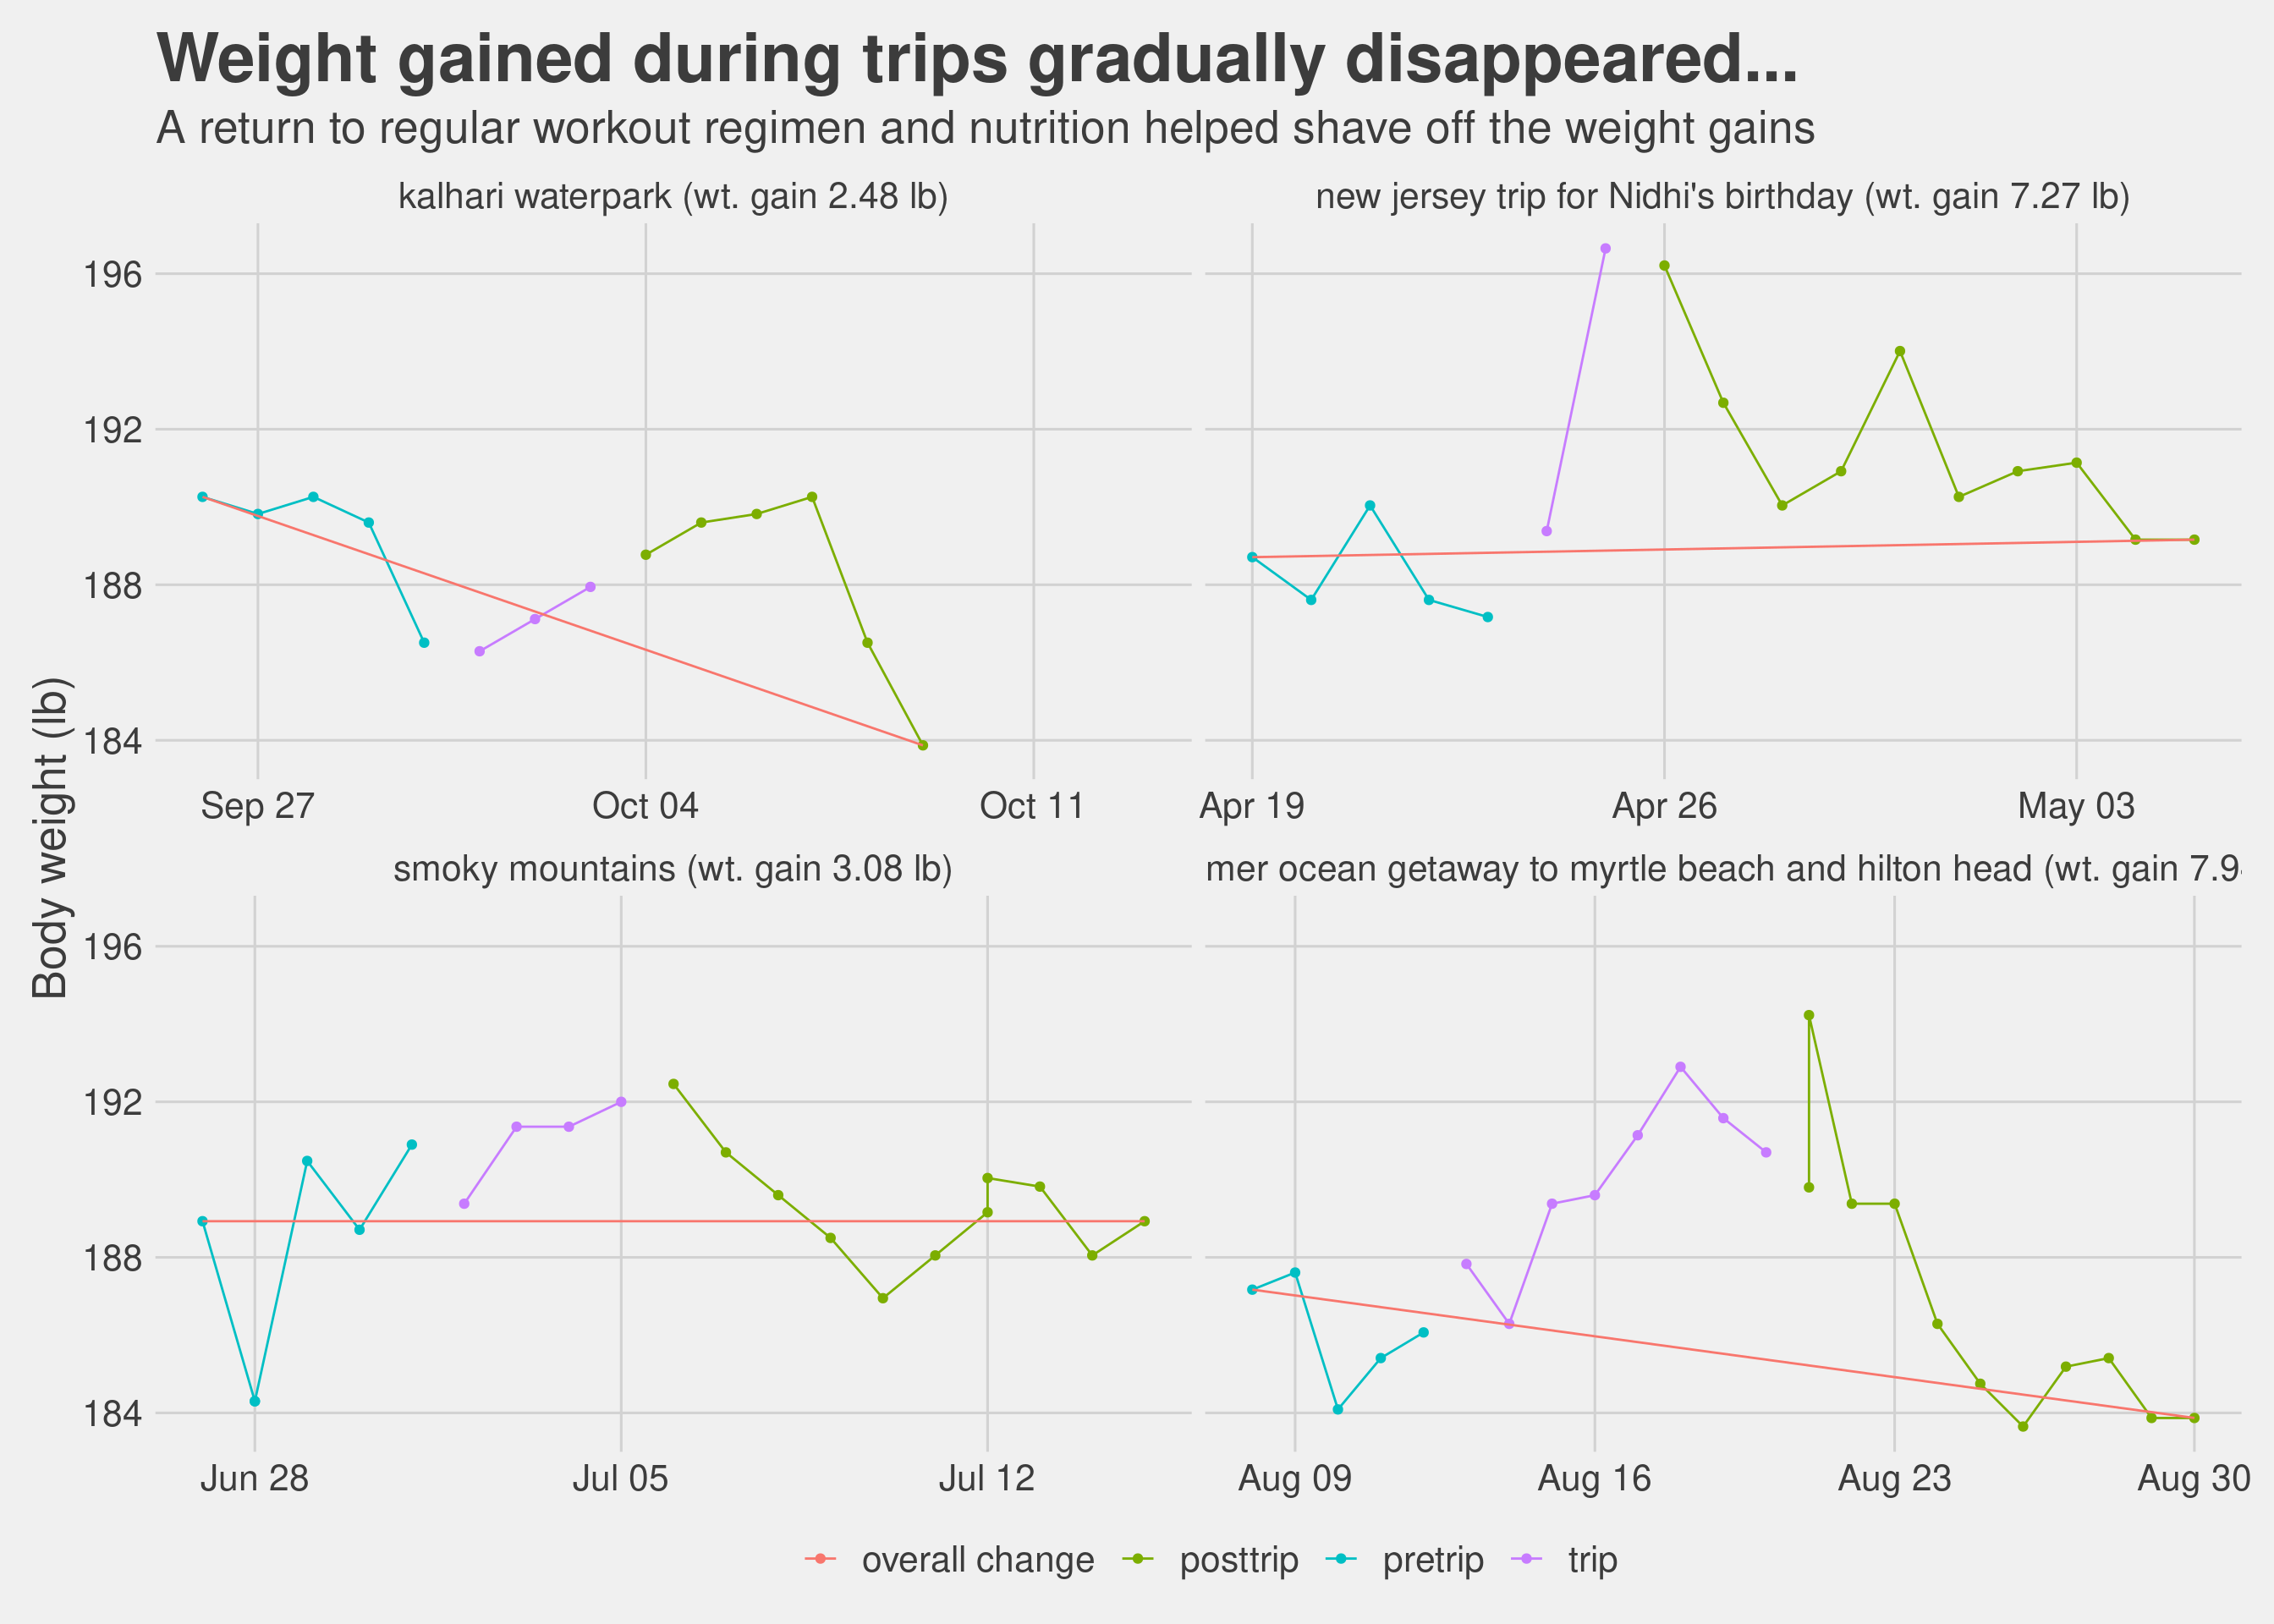
\includegraphics{bookdownproj_files/figure-latex/unnamed-chunk-24-1.pdf}

\hypertarget{chapter-7-at-a-glance}{%
\section{Chapter 7: At a glance}\label{chapter-7-at-a-glance}}

\begin{center}\rule{0.5\linewidth}{0.5pt}\end{center}

\begin{enumerate}
\def\labelenumi{\arabic{enumi}.}
\item
  Food composition changes as the extra weight comes off and the demands of the workout increase. I eat less protein than before and regular Indian food (daal, roti, sabzi) for dinner.
\item
  We choose eating two big meals a day rather than multiple small meals through the day. Skipping the breakfast helps with intermittent fasting.
\item
  The lunch is still a protein, fiber and a good fat rich salad. Avoiding carbs at lunch time helps avoid the lethargic feeling during the afternoon.
\item
  Dinner now has a higher carb content than before (please do not delay dinner beyond 7:30pm) which helps with a good night sleep and fueling the workouts the next morning.
\item
  A consistent regimen of the workout and healthy eating helps shave off the extra pounds from the social gatherings and vacations.
\end{enumerate}

\hypertarget{fasting-for-overall-health-and-longevity}{%
\chapter{Fasting for overall health and longevity}\label{fasting-for-overall-health-and-longevity}}

Growing up, fasting for religious reasons on special days was very normal. We did it several times a year as a family. The focus was not so much on the health benefits but more on the spiritual side of it (abstinence from food helps brings the focus inwards, maybe). As I grew older, I started looking at these fasts more and more as an opportunity to test self-control, with work, travel and other day to day life situations it was always somewhat of a challenge. Even though the fasts themselves did not involve going without food for long hours (certainly not days), you could always eat something from the allowed set of food items. It was still a challenge, nonetheless.

One thing that my fasting experience growing up taught me that ``hunger comes and goes, and it always gets better'' especially with the multi-day fasts (again, there were always some allowed food items such as fruits, nuts, certain vegetables), I knew the first day was the most difficult and by the 3rd day while the mind certainly wanted certain food, the body was not missing anything and in fact felt better than it did before fasting.

Different cultures around the world have since times immemorial have traditions of fasting, so in that sense the modern-day interest in fasting is not something brand new, although what is new is looking at fasting through the lens of science, specifically that of clinical trials. Fasting has profound effects on the body and the mind. While we did not go beyond a 4-day fast, but even that I would liken it, at least to some extent, to a dopamine fast where you are surrounded by abundance (of food in this context) but you deprive yourself of it and in doing so reset the brain's reward circuitry. After the fast any food that you get to eat is experienced as the most satisfying food you have ever eaten!

I am going to discuss two types of fasting routines in this chapter, first is ``Time Restricted Feeding'' or the so called ``intermittent fasting'' and second is extended multi-day fasts (such as a 48 hour or 72-hour fasts).

\hypertarget{time-restricted-feeding}{%
\section{Time Restricted Feeding}\label{time-restricted-feeding}}

Chances are that you have heard about Time Restricted Feeding (TRF) or as everyone likes to call it ``Intermittent Fasting''. As the name suggests you define a feeding window in which you eat all your food for the day and try to stick to it both for the duration and the time of day. So, for example a 12:12 TRF could be eat between 8am to 8pm or said another way do not eat anything between 8pm to 8am. You could also change it to 9am to 9pm while still maintaining the 12-hour fasting and feeding window but shifting the time of day when that window occurs. Usually it is advisable to stop eating 2 (preferably 3) hours before bedtime so an 8am to 8pm window is convenient. The feeding window could also be 8 hours instead of 12 in which case it becomes a 16:8 fasting and feeding cycle. In a 16:8 TRF one could wait till noon before eating anything and thus the feeding window is from 12pm to 8pm. Some people also do the 22:2 which only leaves time for ``one meal a day'' or OMAD as it is commonly called. Finally, there is also a 5:2 routine in which people eat regularly for 5 days and then eat very little for 2 days.

My own experiments with TRF have been that I started with 12:12 and then have graduated to 16:8 and feel very good doing it. The thing that drew me towards intermittent fasting was that it just seemed natural and tied to conventional wisdom I grew up with i.e.~stop eating well before bedtime and do not eat within an hour or two of waking up. So, 2 hours before bedtime and 2 hours after waking up combined with 8 hours of sleep translates to 12:12 intermittent fasting. Easy. Not quite. Over the years, I had become very used to grabbing an after-dinner snack while working late-nights, I now believe that the late-night snack and the lack of sleep were probably the root cause of me putting on so much weight. It took a little bit of effort to avoid the post dinner snack, sometimes I had a protein bar if I really felt like eating something or half a cup of almond milk, slowly but surely, my body adapted, and I no longer needed that snack. In fact, now it is the opposite, if I eat a late dinner, sometimes I wake up in the night feeling extremely hungry, even though I had just eaten a few hours ago.

In early 2021, I had somewhat of an epiphany. I was dealing with multiple work-related crisis and it just so happened that I ended up skipping breakfast several times during a two-month period. Since the workouts were with the trainer so I could not skip those (also they were in the morning, although I did skip one or two) but I could skip breakfast, simply because I did not want an interruption. What I realized later, was that on those days when I had skipped breakfast but did my workouts as planned, my focus was razor sharp, I could concentrate for longer duration and overall just felt better. I decided to continue the experiment even when there was no crisis and it was just a normal day and realized I indeed functioned better and had more energy if I did not eat until noon or 1pm. I decided to formally switch to 16:8 where I have my first meal of the day (which would technically be my break-fast but is my lunch) between 1pm to 2pm and then have my dinner between 7 to 8pm (occasionally 8.30pm). I will admit that when I first started this extended experiment, I used to think after finishing my dinner that ``Oh my God, am not going to be able to eat anything until lunch time tomorrow, really???'' but as I realized it was actually not that difficult. I have been doing the 16:8 for most of 2021, and I find it suits my lifestyle perfectly.

While there are studies that document results from clinical trials (in both rats and humans) showing benefits of TRF both in terms of weight loss and overall health but to me it was just something that intuitively made sense. I thought why I would want to snack every now and then and keep spiking my insulin levels, feel lethargic and then as a result want to snack more and then the cycle just continues. The best part for me was that if done in accordance with our natural circadian clock it just seemed natural and not an add on activity that I had to think about doing.

I also tried the 22:2 a few times, it was fine but not something I enjoyed. Having said that, I never tried it long enough, just a day here or a couple of day there. Admittedly, I did use the 22:2 as some form of a damage control mechanism after say a weekend of eating out and late-nights and it did work, but I felt it did not come naturally to me like the 16:8 so I did not pursue it. I never tried that 5:2, because it made no sense to me.

I cannot end this section without saying please read this excellent book called ``The Circadian Code'' by Dr Satchin Panda, it will provide you evidence-based reasoning you need to try out TRF.

\hypertarget{multiple-day-fasting}{%
\section{Multiple day fasting}\label{multiple-day-fasting}}

It was probably through some YouTube recommendations that I stumbled upon the topic of longer multi-day fasts, more specifically, ``multi-day water fasts''. These fasts could be anywhere between 1 day to several days where you eat no food and only water (+ electrolytes) was allowed. Both me and Nidhi were very keen on trying this. I had fasted for multiple days before (not water fast though and certainly not for multiple days) but she had not. So we met with a naturopathic doctor and asked her about it, she said she wanted to get some bloodwork done to make sure she did not see anything which would make her say no. Long story short, everything turned up OK in the bloodwork and she really encouraged us to do a multi-day water fast. We could drink tea, coffee and electrolytes but no milk (no dairy, but a little bit of almond milk was OK) and of course no sugar. Basically, anything that had calories was out.

I had not heard about this word called ``autophagy'' which literally means ``self-eating'' before I stumbled upon videos, podcasts and articles about multi-day fasting and it being a means to trigger autophagy. Google ``autophagy and noble prize'' and you will find a detailed presentation on autophagy. As I understand it, multi-day fast are one of the means of triggering autophagy which allows the body to remove and recycle damaged cellular material and thus providing multiple health benefits such as longevity and improved mental health. Fasting is not the only way of triggering autophagy, good sleep, exercise, certain foods, would all trigger autophagy. Fasting though, is one of the most effective way of triggering autophagy as supported by multiple studies (\href{https://www.ncbi.nlm.nih.gov/pmc/articles/PMC6627766/}{this}, \href{https://www.ncbi.nlm.nih.gov/pmc/articles/PMC3106288/}{this}).

We started with a 2-day water fast, and then gradually increased it to 3-days and finally to 4-days. While it is not easy, but it is certainly not as difficult as it might sound. To anyone wanting to try it, I would suggest easing into it, if you have never fasted before you will be miserable on the first day of the fast. Some amount of metabolic flexibility is required for a multi-day fast, in other words the body should have some experience in producing energy by burning something other than carbohydrates, namely fat. Start with intermittent fasting, a 12 hour fasting and feeding window, after a couple of weeks on 12:12 change it to a 16:8 routine where you fast for 16 hours, stay there for a few weeks, then try a few days of 22:2 and having done that you will be in a mental frame where the idea of skipping food for a whole day and going to sleep empty stomach would not appear daunting. It is always a moment of self-realization to find out for the first time that you can survive without eating for a whole day and feel just fine the next morning. If someone is used to eating 3 meals a day with snacks in between, they cannot just decide and start a multi-day fast, you do not want it to be a test of will power, you want to work with your body and gradually ease into it. We have been doing multi-day fasts every month since April 2021 (it is November 2021 as I write this).

To be clear, when I mention a 2-day fast I mean a 48-hour period without food, so if we are fasting Monday and Tuesday, the fast begins at say 8pm on a Sunday and then we do not eat anything until 8pm on Tuesday. Now technically, we are still not fasted when we sleep on Sunday night and so should we count the 48 hours from say Monday morning, maybe? Autophagy gets triggered by anywhere between 18 hours to 4 days, so I guess somewhere during those 48 hours we would have started getting the benefits.

\textbf{\emph{NOTE}}: Please consult with your doctor before doing any type of fasting, we certainly did.

Here is a quick primer on how to go about a multi-day and what to expect during the fast.

\hypertarget{how-to-prepare-for-the-fast}{%
\subsection{How to prepare for the fast?}\label{how-to-prepare-for-the-fast}}

The most important thing to do is somewhat counter intuitive and that is not to eat too much during the last meal before the fast. One would think that I am going to be without food for the next 48 to 72 hours so let me stock up, while the thought might be correct, but in reality, the body is already stocked up which is what all the stored body fat is. The body is going to use that body fat for energy when it is does not get food, that is what we want. Also, we try to be very diligent about reducing our carbohydrate intake a day before the fast starts, helps us feel less hungry on the first day of the fast (hunger is only a first day problem, no really).

In terms of what liquids other than just plain water that you can consume during the fast, make sure you have tea, coffee, sparking water, electrolytes (make sure 0gm of sugar, of any kind, some brands don't mention sugar but say sucralose, you don't want that). Also lemons, for lemon juice if you like that and most importantly salt. No coconut water please, because it is naturally sweet, and we want to completely avoid carbohydrates. I did have some (maybe a teaspoon) of almond milk during some of my fasts but I do not do that anymore.

Finally, remember, hunger comes and goes, and your body has enough stored fat to survive a few days without food.

\hypertarget{day-1-of-a-72-hour-fast}{%
\subsection{Day 1 of a 72-hour fast}\label{day-1-of-a-72-hour-fast}}

Day 1 is the hardest! By the afternoon, you start feeling hungry, late afternoon could be difficult, if this is your first time might experience with some mild headaches. Then the hunger subsides and goes away. Drinking electrolytes really helps (again, make sure no sugar because otherwise it could make you feel even worse), it would reduce hunger and help with the headache because of all the salts content (sodium, magnesium, potassium).

Make sure you drink water, tea, coffee, it all helps. It is important to continue with your regular lifestyle, we did. Unless of course your regular lifestyle involves strenuous physical activity, you should be fine. I had some instances where I had to do a lot of talking (work, meetings) and that does take a lot of energy, must keep that in mind while scheduling the fast.

I do my regular workouts on day 1 and day 2 of the fasts, maybe at somewhat reduced intensity but I do not skip my workouts. In fact, I feel better (more energetic) after the workouts.

By evening, I am feeling sleepy and want to go to bed early. This is a good idea because when you are sleeping, you are not thinking about food. More than hunger, it is the act of preparing food for the family, the aroma of food that makes you think ``tell me again why I anot not eating this?''. To be honest, the first day is tough.

\hypertarget{day-2-of-a-72-hour-fast}{%
\subsection{Day 2 of a 72-hour fast}\label{day-2-of-a-72-hour-fast}}

When you wake up the second morning, you would be feeling refreshed after the sleep and surprisingly not hungry. You can then go about your day as normal, if there is no strenuous physical activity involved and not a lot of talking, you would feel fine, certainly much better than day 1 and maybe even better than when you were not fasting.

The afternoon would probably bring some hunger, but now you know how this plays out, the hunger will subside in an hour or so. Electrolytes, tea and coffee should all help.

A different feeling that we had on day 2 was a strange feeling of emptiness in the stomach, it was not hunger but a strange but entirely expected feeling of missing food. Energy levels are fine, you are not hungry, but you miss the act of eating because that is an intrinsic life activity. That feeling, of just missing food even when not hungry, is probably what would cause you to say, ``ok I don't want to do this any longer''. If you are doing a 48-hour fast and you started counting the hours since dinner two days ago then day 2 is not hard because you know that in a few hours you are going to be eating. If you are going to continue for another day or two, then yes, you want to keep yourself busy with regular work and go to sleep early at night, that is what we do.

An interesting thing that happens (and for some this might happen earlier on day 1 itself) is that you start feeling cold. This is because there is no metabolic activity going on to digest food, so there is less heat produced and therefore you would feel the palms of your hand to be cold.

\hypertarget{day-3-of-a-72-hour-fast}{%
\subsection{Day 3 of a 72-hour fast}\label{day-3-of-a-72-hour-fast}}

If this is your final day of fasting, then Day 3 is easy because your destination is in sight. If this is not your final day then day 3 is very much like day 2 i.e.~you must contend with ``boredom of not being able to eat'' and random thoughts of ``Ok enough, I just want to pick up this banana and eat''.

By day 3, you get used to not feeling hungry, no headaches, probably a little bit low on energy levels but nothing extraordinary.

Day 3 often comes with questions such as ``remind me again why am I doing this?'' and at that time it is just a question of running out the clock.

\hypertarget{how-to-open-a-fast}{%
\subsection{How to open a fast?}\label{how-to-open-a-fast}}

The first food item, rather the first meal, after a multi-day fast feels like heaven. You realize what does food mean to the soul, not just to the body because you now know the body can do just fine for a few days without food. The fast brings about such a big reset to the idea of ``good food'' that it is difficult to describe, whatever you eat as part of your first meal is good food.

We usually open our fast with a soup, something light such as a vegetable soup made from beets, spinach and tomato served with a little bit of butter. Followed by some nuts and dried fruits and then a light dinner. It is difficult to eat too much after a fast. You do not want to give another shock to your digestive system which is just getting used to not having to digest any external food by suddenly eating a whole lot of carbs.

\hypertarget{the-morning-after}{%
\subsection{The morning after}\label{the-morning-after}}

The weighing scale does show us lighter by several pounds (anything between 4 to 7 pounds) but this weight loss is not permanent and water fasts are not meant to be a weight loss protocol. Said a different way, water fasting is not meant to be a detox after a vacation that added a few extra pounds.

We generally feel great with no residual impact from the fasting.

\hypertarget{our-72-hour-fasting-experience}{%
\subsection{Our 72-hour fasting experience}\label{our-72-hour-fasting-experience}}

During one of our fasts I decided to meticulously record all the data on a per hour basis so that we had actual data recorded in real time to reflect what we were experiencing: were we hungry, sleepy, had headaches and also what did we drink. Here is a link to the Google sheet I created to track this, you can download it \href{https://docs.google.com/spreadsheets/d/1qGM7gJ8zdBPTngD0HHkutP83-kCZx_erLRIak5hs5Lk/edit?usp=sharing}{from here} and use it to track your own fasting experience.

We mostly had normal energy levels, sometimes mild headache and almost no extreme hunger pangs. About a third of those hours were spent sleeping! I should note that this data was probably from our 3rd attempt at multi-day fasting, I believe we have gotten better at it and do not experience any headaches (not even mild ones) at all now.

\begin{figure}
\centering
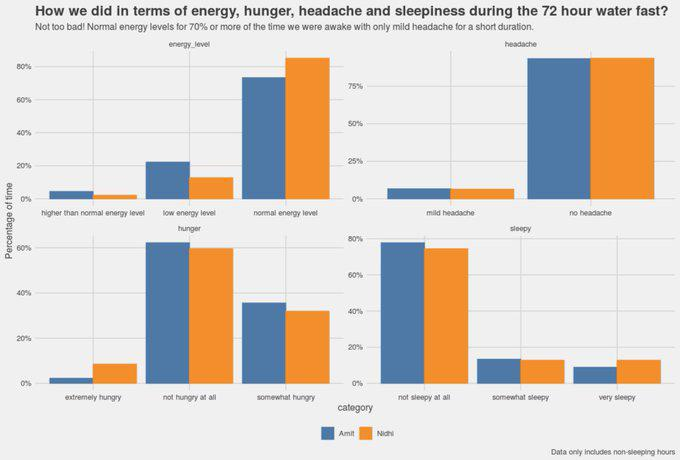
\includegraphics{pictures/fasting1.jpeg}
\caption{fasting experience}
\end{figure}

A multivariate analysis examining a combination of energy level, hunger and sleepiness is more interesting. Did we feel low energy, very hungry and very sleepy at the same time? Surprisingly, no! The high energy levels correspond to the hour just after a workout.

\begin{figure}
\centering
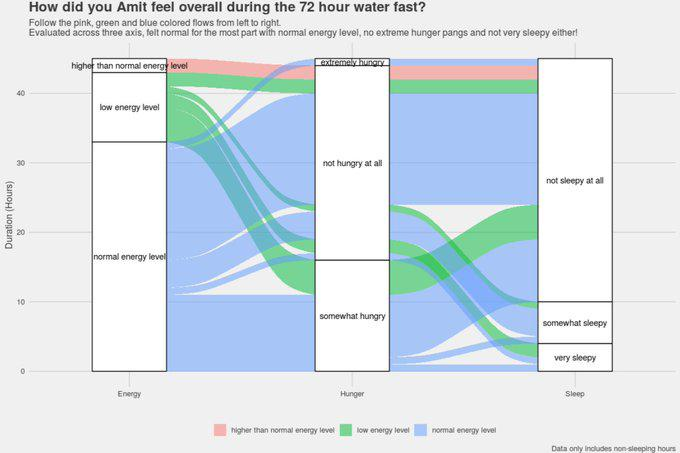
\includegraphics{pictures/fasting2.jpeg}
\caption{multivariate analysis of fasting experience for Amit}
\end{figure}

Same for Nidhi as well, no case of hunger pangs combined with low energy and feeling very sleepy. While a 72-hour water fast is no walk in the park, it was definitely not the case that we felt we would collapse going without food for a few hours.

\begin{figure}
\centering
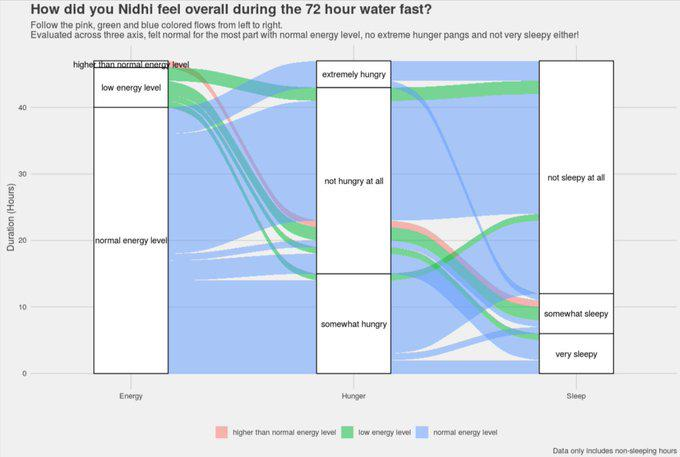
\includegraphics{pictures/fasting3.jpeg}
\caption{multivariate analysis of fasting experience for Nidhi}
\end{figure}

Our fast was not a water only fast. While I drank a variety of beverages other than just water, Nidhi mostly stuck to water and tea.

\begin{figure}
\centering
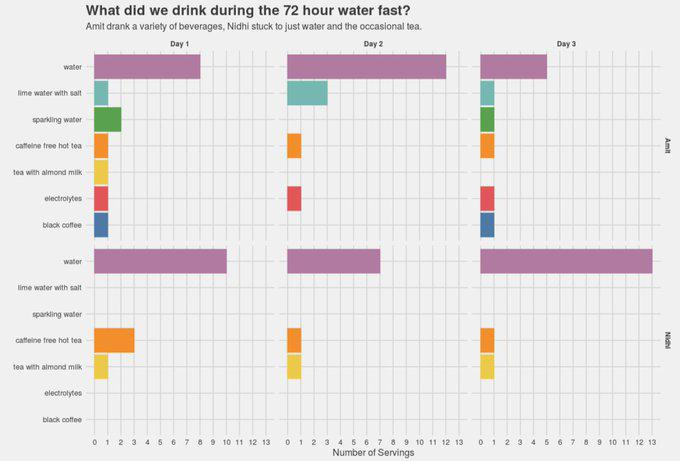
\includegraphics{pictures/fasting4.jpeg}
\caption{What did we drink during fasting}
\end{figure}

\hypertarget{closing-thoughts-on-fasting}{%
\section{Closing thoughts on fasting}\label{closing-thoughts-on-fasting}}

We would like to do a longer fast, something like a 5 to 10 day fast but we also have work to do and kids to attend to and friends to meet (and eat with) all of which make it difficult to sustain a fast for a longer duration (4 days is the maximum that Nidhi tried, I did not try more than 3 days). We get our bloodwork done every few months and several biomarkers show marked improvements but then it is hard for us to say how much of it is due to fasting and how much is due to overall lifestyle changes. Tests for autophagy are not yet common and we certainly have not got one done, an objective quantitative measure would certainly help provide an impetus for an extended multi-day fast.

Some of our friends also tried out a 48 hour fast (I hope at least in part based on our experience) and they also had similar experience as us, once the first day was over, it was not that hard.

I will close this chapter by citing an anecdote of my own. I believe that the multi-day fasting helped to completely clean up a painful skin condition that had developed in the sole of my foot. While I have no scientific proof that it was indeed the fasting that cured it, but I can say for sure that it got better after every fast and was healed after a few fasting iterations. All this while the podiatrist was not having much success in treating my condition and the next step in that line of treatment was to get an MRI done (I had already got an ultrasound done which did not reveal anything), which I did not get done and thankfully did not need ultimately. The body knows how to heal itself; we just need to give it some help. Just so that I do not come across as promoting quackery, please always consult your doctor for all medical conditions and before starting on any fasting or dietary regimen.

\hypertarget{chapter-8-at-a-glance}{%
\section{Chapter 8: At a glance}\label{chapter-8-at-a-glance}}

\begin{center}\rule{0.5\linewidth}{0.5pt}\end{center}

\begin{enumerate}
\def\labelenumi{\arabic{enumi}.}
\item
  Revisiting the traditions of fasting through modern science offers new insights into how fasting helps heal our body and mind.
\item
  Intermittent fasting or time restrictive feeding has benefits in terms of weight loss as well as improvements in general health. A 12:12 fast that allows with the body's circadian clock should be within reach for most people.
\item
  A multi-day fast triggers autophagy which is a process by which the body removes and recycle damaged cellular material thereby improving health and promoting longevity.
\item
  When done with proper preparation a 2 to 4-day water fast (that we did) was not as difficult to do as it might appear at first thought. It is natural to think that such a fast would involve a lot of hunger pangs, headaches and lack of energy, but as we discovered, that was not the case for us.
\end{enumerate}

\hypertarget{breathwork}{%
\chapter{Breathwork}\label{breathwork}}

\textbf{NOTE}: In this chapter I refer to specific people and books, I would like to put it on record that this book is not endorsed by them, they probably do not even know that this book exists. Whatever I write here is my understanding of what I read from their books or saw from their videos. Anything you read in these pages or elsewhere in this book is meant for informational purposes only, it is not medical advice. You are responsible for your health, not me, please consult your doctor before starting any new protocol.

\begin{center}\rule{0.5\linewidth}{0.5pt}\end{center}

I am a software developer by training. One of the things that I learnt early on was that if you wanted to optimize a computer program so that it runs faster, then you optimize the one module that in itself might appear trivial and hidden from the user visible functionality but was performed repeatedly and therefore any improvement in it had a multiplicative effect on the performance of the overall program. Breathing is that hidden module in the human system. We breath about 20,000 times a day on an average, it is an involuntary action for the most part and even a small improvement in breathing can have a huge impact on our health, both mental and physical.

When I started training, our trainer told us about breathing patterns appropriate for a particular exercise but I did not focus on that too much because I was so new to workout and exercise and my forms were so clumsy that adding a breathing pattern to an exercise was just one thing too many. As my forms improved, some basic movements and bracing became a part of habit and I did not actively need to be aware of them, they just happened, maybe that freed up some of my brain to focus on the missing link i.e.~breathing. In any case, that is hindsight. It all started with me reading James Nestor's wonderful book called ``Breath: the new science of a lost art''. I think I stumbled upon some YouTube video about it, I don't remember for sure but as I read a little bit about the book, I was convinced I need to read it. I am so happy that I did. The book has many references to ancient Indian breathing practices, and I asked myself ``why am I not trying some if not all of this?''. After finishing that book, I read Dr Belisa Vranich's book ``Breathing for warriors'' and devoured every YouTube video and podcast I could find about breathwork.

\hypertarget{two-fundamentals}{%
\section{Two fundamentals}\label{two-fundamentals}}

The two most fundamental things that you can (and should) so are nasal breathing and horizontal breath or belly breathing. First up, the mouth is not meant to be the primary organ for breathing, the nose is, unless you are completely out of breath say while doing a hard exercise routine, you should not normally need to breathe through your mouth. Breathing through the nose offers a natural filtering mechanism to keep the harmful things out of your body, prevents dental problems and in general helps keep you calm and relaxed. I remember growing up, I used to have frequent colds and used to breathe through my mouth a lot and my mother had a very tough time constantly reminding me (often in public) to keep my mouth closed. As I grew up and my immunity got better, the frequent colds went away and while I did not breathe through my mouth as much, but it was not something that I paid attention to, not sure most people do.

After reading James Nestor's book I started being conscious about nose breathing and any time I found myself breathing through the mouth I immediately switched to nose breathing. Then one day I decided to see if I could train with my mouth closed and only breathing through the nose. I barely made it past the 5-minute warmup before I had to open my mouth for breathing. I persisted, and it got better, in a couple of weeks I could finish a 10-15-minute strength training portion of the portion of the workout which usually involved heavy deadlifts, back squats or other compound exercises. Whenever I did heavy cardio, such as sprints, a few calories on the assault bike, burpees and such I had to open my mouth. I knew I was getting better though. A couple of months into the nose breathing and I could finish the cardio portion as well. Today (about 6 months in), I am able to complete the entire 50-60 minute workout without having to breathe through my mouth, and more importantly, I do not even feel the need to (of course talking to the trainer or having a sip of water means I do breath through my mouth in between sets). I no longer feel out of breath while working out, my heart rate remains under 140 even during intense cardio and my endurance levels have improved tremendously.

The other fundamental is horizontal breathing or belly breath or diaphragmatic breathing. Put simply, a belly breath means expanding your belly as you inhale so that your lungs push your diaphragm down and contracting your belly while exhaling so that your diaphragm expands and moves upwards. This is best understood by seeing some visualizations and videos, there are many, but I would recommend Dr Belisa Vranich's books. It takes some practice to unlearn how we have been breathing all this while and how we used to breath in early childhood.

\hypertarget{our-breathwork-routine}{%
\section{Our breathwork routine}\label{our-breathwork-routine}}

Here are the specific practices I follow and benefit from.

\hypertarget{the-4-7-8-breath}{%
\subsection{The 4-7-8 breath}\label{the-4-7-8-breath}}

To improve sleep, we use the 4-7-8 breathing technique just before sleeping. It is extremely relaxing and helps to fall asleep so much faster. I learnt it from watching Dr Andrew Weil's video recommended from James Nestor's book. We do it once a day right before sleeping, or any time during the day if the stress level gets high. The technique is simple, touch the roof of your mouth with your tongue, inhale for 4 seconds, hold for 7 seconds and then exhale for 8 seconds, repeat this 4-7-8 cycle 4 times. Takes less than 90 seconds total. As with everything else, takes several weeks of consistent practice to see the benefits. There is an app for the 4-7-8 breath, it does the time tracking for you so that you only must focus on breathing.

\hypertarget{the-pre-workout-practice}{%
\subsection{The pre-workout practice}\label{the-pre-workout-practice}}

I got this protocol from a Brian Mackenzie's video recommended from James Nestor's book. It goes like this:

\begin{enumerate}
\def\labelenumi{\arabic{enumi}.}
\tightlist
\item
  Cycle 1
\end{enumerate}

\begin{itemize}
\tightlist
\item
  Repeat 5 times

  \begin{itemize}
  \tightlist
  \item
    2 second inhale
  \item
    2 second exhale
  \end{itemize}
\item
  20 pulse breaths
\item
  20 second exhale hold
\end{itemize}

\begin{enumerate}
\def\labelenumi{\arabic{enumi}.}
\setcounter{enumi}{1}
\tightlist
\item
  Cycle 2
\end{enumerate}

\begin{itemize}
\tightlist
\item
  Repeat 5 times

  \begin{itemize}
  \tightlist
  \item
    3 second inhale
  \item
    3 second exhale
  \end{itemize}
\item
  20 pulse breaths
\item
  20 second exhale hold
\end{itemize}

\begin{enumerate}
\def\labelenumi{\arabic{enumi}.}
\setcounter{enumi}{2}
\tightlist
\item
  Cycle 3
\end{enumerate}

\begin{itemize}
\tightlist
\item
  Repeat 5 times

  \begin{itemize}
  \tightlist
  \item
    4 second inhale
  \item
    4 second exhale
  \end{itemize}
\item
  20 pulse breaths
\item
  20 second exhale hold
\end{itemize}

This protocol stimulates the sympathetic nervous system so that the body and mind are prepared for a stressful activity i.e.~a workout routine. I do this prior to my workout. When I first started doing this, I did this with some healthy skepticism as to how much benefit I would get out of it even though I understood why it should help (release of adrenaline and noradrenaline). Over a period of a few weeks I realized it really made a difference in that my workouts did not seem as strenuous even though I was lifting heavier than before and more specifically I didn't feel totally enervated after a 12-minute EMOM. On some off chance that I forget doing this I immediately feel a difference during my workout and realize that it is because I missed my pre-workout breathwork and then I go back and do it.

\hypertarget{breathing-pattern-during-the-workout}{%
\subsection{Breathing pattern during the workout}\label{breathing-pattern-during-the-workout}}

Other than not breathing through the mouth unless necessary, I follow a simple rule: exhale while exerting effort, inhale when not exerting effort. This seems counter-intuitive, for the longest time I used to breath in the opposite way, so for example, if I was doing a push press I would inhale while pushing up. As I now understand that is the exact opposite of what I should have been doing. So now, before doing a push press, I take a deep ``belly'' breath, try to feel the air filling up my lungs and pushing outwards 360 degrees in my belly (I know this sounds abstract, but give it a try) and then press with everything tight and the air in the belly still supporting all the weight that I am pressing. I exhale slowly when I bring the barbell down after completing the press. Sometimes, when I really need to find that last bit of energy (around the 3rd rep of the 5th set) I would probably exhale slowly while pressing and a small inhale at the top but generally I try to avoid that. Deadlifts are similar, I take one last deep breath with my hands on the trapbar handles and the body in position, complete the lift, slowly put the trapbar down and then breath again. Occasionally, I would do an inhale at the top of the lift.

Having the air inside creates stability and gives support to the spine for the lift. It makes a world of difference.

\hypertarget{inversions}{%
\subsection{Inversions}\label{inversions}}

Chances are you may have seen a Yogic asan called ``Sheershasan'' or an ``inverted headstand''. There are numerous benefits of doing an inversion (there are several variants of it) such as increased blood flow to the brain (improved cognition), increased core strength, moving the lymphatic fluids to the upper half of the body (since we are inverted) to get rid of toxins from the body but at the same time it is also an exercise for the diaphragm. Just like exercises for the muscles we can see, such as curls for the biceps, the inversion is an exercise for the diaphragm which is a muscle that we do not see. The diaphragm is the major muscle of respiration and can also be made stronger by doing specific exercises, just like any other muscle.

I use a specific contraption called the feetup trainer that makes doing an inversion easier.

\hypertarget{the-physiological-sigh}{%
\subsection{The physiological sigh}\label{the-physiological-sigh}}

This is one of the quickest way to engage your para-sympathetic nervous system (the so called ``rest and digest''). In a way this is the opposite of the protocol I practice pre-workout. Engaging the para-sympathetic nervous system makes us less aroused and therefore less anxious and calmer. Life throws up situations and many times we react to things in ways we know are counter-productive but still we cannot stop ourselves. This protocol comes in handy in such situations. The protocol is very simple and reminds me of how small children sob, take two pulse inhales through the nose and then one long exhale through the mouth, repeat 3 to 5 times. At a physiological level what this protocol is doing is offloading the maximum amount of carbon dioxide.

I would refer you to Dr Andrew Huberman's podcast for understanding the biology behind this protocol.

\hypertarget{taping-the-mouth-while-sleeping}{%
\subsection{Taping the mouth while sleeping}\label{taping-the-mouth-while-sleeping}}

I tape my mouth while sleeping. It is just a small tape put vertically over the center of the lips. It is to ensure that I do not breath through the nose even while sleeping. I know it sounds at least a little bit weird, but it has improved the quality of my sleep. Even with fewer hours of sleep I feel refreshed when I wake up (I am not suggesting this as a way of getting by with less sleep, certainly not, I wish everyone is able to get a good 8-hour sleep). The first time I tried it, I had to take it off after a couple of hours, but then the next day it was fine and from then on, I haven't slept a night without the tape on.

\hypertarget{chapter-9-at-a-glance}{%
\section{Chapter 9: At a glance}\label{chapter-9-at-a-glance}}

\begin{center}\rule{0.5\linewidth}{0.5pt}\end{center}

\begin{enumerate}
\def\labelenumi{\arabic{enumi}.}
\item
  There are several breathwork protocols that we can easily incorporate in our daily lives to improve sleep, workout performance and reducing anxiety.
\item
  The 4-7-8 protocol, the pre-workout protocol for engaging the sympathetic nervous system, the physiological sigh for reducing anxiety are some of the techniques I use.
\item
  Please lookup the people and books I mentioned in this chapter, they are all very worth of your time.
\end{enumerate}

\hypertarget{stream-of-consciousness}{%
\chapter{Stream of Consciousness}\label{stream-of-consciousness}}

Here is a collection of some ``stream of consciousness'' topics that I wanted to convey but did not fit into any of the other chapters so here they are all in a chapter of their own.

\hypertarget{the-murph-challenge}{%
\section{The ``Murph'' Challenge}\label{the-murph-challenge}}

In May of 2020, during one of our Zoom workouts, our trainer just casually mentioned that they were doing this challenge in a couple of weeks where they would do a ``1 mile run, 100 pull-ups, 200 push-ups, 300 air-squats and then bookend it with another 1 mile run''. I had just managed to do like 3 push-ups in a row and I almost fell to the ground doing my 4th push-up and blurted out ``in how many days\ldots?''. While this question might seem funny at this time, hand to the heart, it was a serious question when I asked it. Remember this was coming from a person who thought doing 3 straight push-ups was an achievement. I was being told, in a matter of fact tone, that there are regular people who would be able to do what seemed like a test of endurance and strength to me.

The answer to my question, was ``um, some people take an hour and half, but mostly it is done in under an hour, and then we can do modified push-ups also'', so no it was not an event spread out over multiple days. I did not ask further and that topic did not come up again and until about a year later.

By April of 2021, I could do 4 sets of 8 push-ups relatively easily, I had also done 50 push-ups spread over 4 sets with each set going up to failure (so like 15 in the first one, 13 in the second, 10 in the third, 12 in the fourth just to make it to 50). At this time, I could at least comprehend that yes it would be possible for regular folks who had been training for a few years or had trained earlier when they were much younger that doing this kind of a routine would be challenging for sure but not as impossible as it had seemed to me a year ago. When we talked about this challenge again, then I looked up the history behind it and I thought this year both Nidhi and I should be able to do this (see \url{https://themurphchallenge.com/}).

I decided to prepare for the challenge, the last thing I wanted was to show up there and then not be able to complete it. So once a week until the challenge day (Memorial Day) I trained to do a mini murph at home, which included a mile on the rower, followed by 5 sets of 6 pull-ups, 6 push-ups and 6 air-squats (or sit-ups) and then a mile on the rower again. I took 30 seconds break between each set. When I did it the first time, I had no idea how hard it would be, fortunately, it seemed manageable. Why the number 6? Because by that I could only do 6 ``assisted'' pull-ups in a row, doing 8 push-ups seemed hard after the first 2 sets so I wanted to pace myself and so 6 seemed like a nice comfortable number. While I managed to complete the 5 sets that I wanted to, but I also realized that at this pace I would be at it for a very long time. Next week, increased the push-ups to 8, and air-squats to 10 per set. Still Manageable. Reaching up to the challenge day, I was settled into 5 pull-ups, 10 push-ups and 15 air-squats per set, just had to complete 20 sets of this and we would be done.

A few friends of ours were planning a trip to the beach on that Memorial day weekend and that would have meant that we reach home late evening on Saturday and then just show up Sunday morning without a good night's rest. We decided against it, instead had a relaxed Saturday, ate simple carb rich dinner, a mile long post dinner walk, and then went to bed around 9:30pm. Woke up next morning, quick 5 minute morning walk and then showed up in the local park where the rest of the folks from our gym were gathering.

Memorial day 2021 in Clarksburg, MD was a bright sunny day, temperature in the early 50s if I remember correctly. A near perfect day for being outside. We started with the 1-mile run; I had not run a mile before, at least not that I could remember. It was challenging, I think completed it nine and a half minutes. Started with the 5 pull-ups (to be clear, we did jumping pull-ups, I know, not the same thing but hey, even this wasn't a cake either), 10 push-ups and 15 air-squats routine. The energy of seeing people around you doing the same workout rubs on you. I took 10 to 15 seconds breaks between sets, slowly the breaks increased to 20 to 30 seconds and towards the end 45 seconds. Finally managed to finish the 20 sets. The hardest part was the push-ups, 200 push-ups are a lot of push-ups. By the time we finished, most people were already done with their second 1-mile run. I ran half of the last mile and walked the other half. Finally, when I finished, it was a few seconds shy of 60 minutes. I was the last person to finish the challenge, but that part was irrelevant, I was overjoyed that I finished the challenge. A year ago, I was thinking this was a multi-day activity, and here I was drenched in sweat, all done in under an hour!

Next year, I aim to complete the challenge in less than 45 minutes, maybe even 35 minutes, I guess we will find out. Here is a picture of Nidhi and me just after completing the challenge.

\begin{figure}
\centering
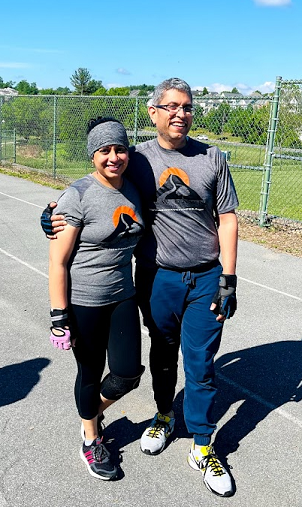
\includegraphics{pictures/murph.png}
\caption{Murph Challenge}
\end{figure}

\hypertarget{my-first-5k-run}{%
\section{My first 5K run}\label{my-first-5k-run}}

Running is not one of my favorite activities, probably because growing up I was never fit enough to run for more than a few hundred meters. As I progressed in my fitness journey, I wanted to explore things I did not think were possible for me and running was one of those things for sure. I wanted to see what all the calories burnt, and minutes spent on the assault bike translate into on a trail. I had run the 1 + 1 mile during the Murph but nothing after that.

We had just returned from an early morning shopping trip on the Friday after Thanksgiving and I happen to notice an Instagram post from our trainer about a 5k run in a park nearby. 5k or 3.1 miles should be manageable, I thought to myself, and if I cannot run all the way then I could always walk. I had started enjoying spending time outdoors and there wasn't really any reason to not do this, so I signed up. The run was next morning.

It was extremely cold and windy the next morning and we were all gathered at the Rachel Carson trail in Brentwood, MD. It was a 5k loop, start from the parking lot, run the loop and finish the run at the same spot. We started together divided into two groups, a group that wanted to run, a group that wanted to walk and enjoy the scenery and then there was me who wanted to start with a run and then fall back to the walker's group if needed. I wanted to run/walk the whole 5k without having to breathe through my mouth and that would also mean run at a comfortable pace so that I did not run out of air and just had to breathe through the mouth. About 800 meters in, I had to slow down and walk, it was not a flat trail and more importantly I had forgotten to do my pre-workout breathwork and I think it was making its absence felt. After walking for a couple of minutes, I started running again and this time, it felt easy, I could run without having to stop. Had to slow down and stop to tie my shoelaces, and the group ahead of me was waiting for the rest of the folks to catch up. Back to running again, then walking a little bit, then running again and before I knew it, I could see the road again and suddenly I could see the parking lot from where we started, I sprinted the last couple of hundred meters.

Took me 30 minutes for the 5k. Not too bad, I thought. I really enjoyed it and I am looking forward to making these short 5k runs a monthly family activity. Here is some data from my watch, for some reason it got the time and duration a little bit wrong but overall it was good to see this data and use it as a baseline for future runs.

\begin{figure}
\centering
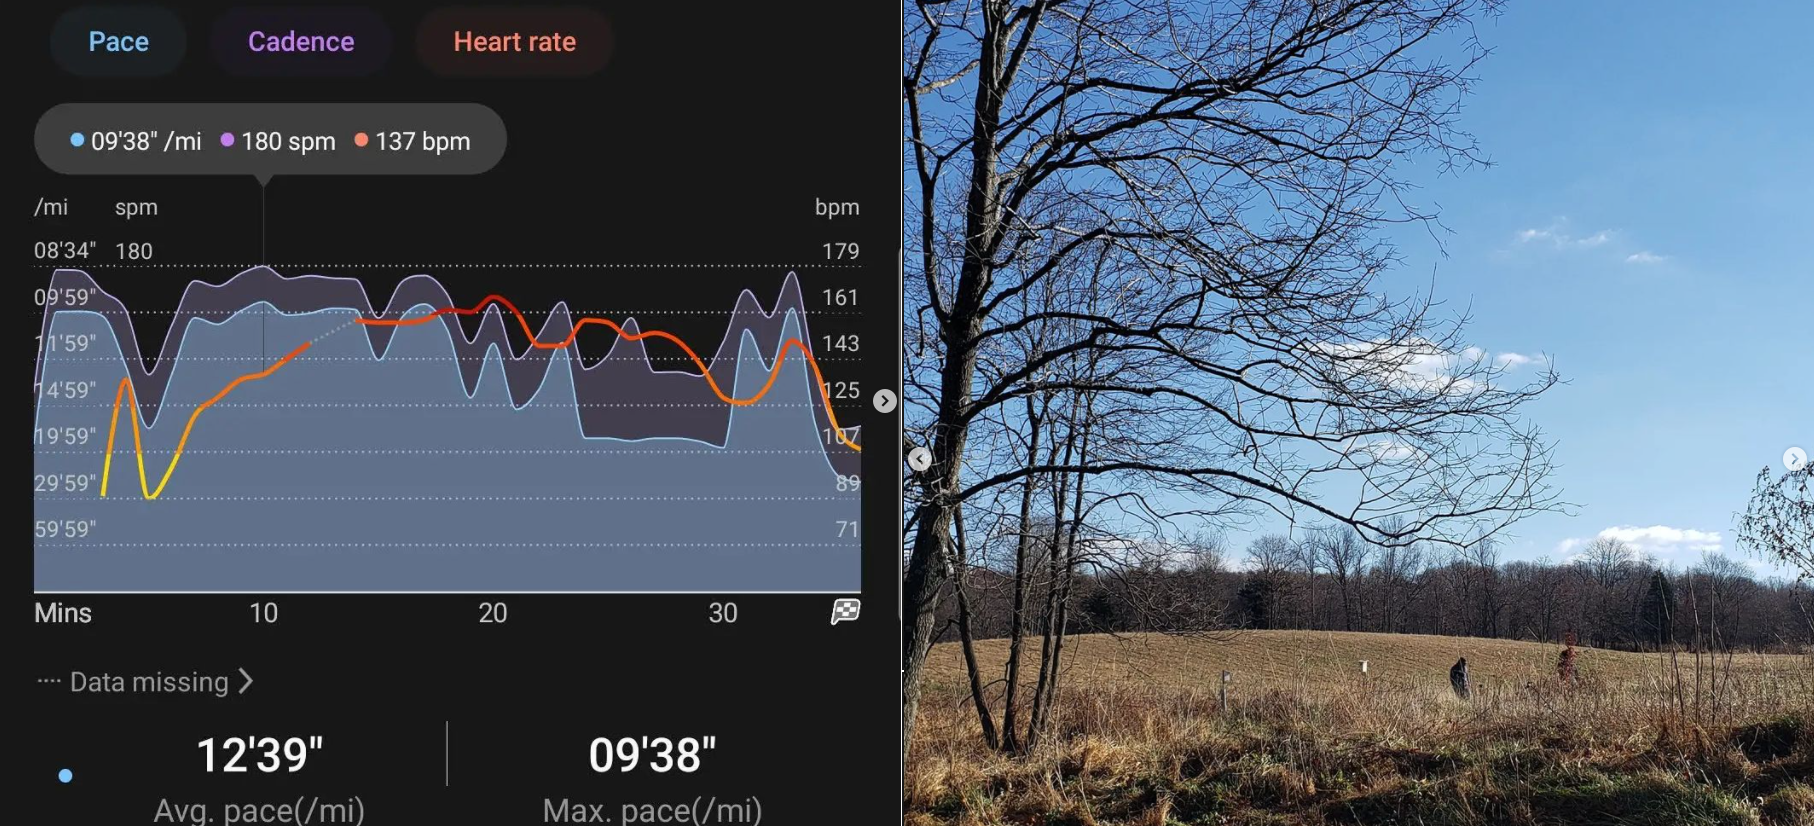
\includegraphics{pictures/5k.png}
\caption{watch data for 5k run}
\end{figure}

\hypertarget{carbohydrates-are-not-your-enemy-and-protein-not-your-only-friend}{%
\section{Carbohydrates are not your enemy and protein not your only friend}\label{carbohydrates-are-not-your-enemy-and-protein-not-your-only-friend}}

Like me you might have friends who lost a significant amount of weight by switching to a high protein and low carb diet, you might be thinking, should I do that too?

Well, I can say this from personal experience, a high protein low carb diet would almost certainly make you lose weight (all standard disclaimers apply, I am not recommending any diet here, nor offering any medical advice, please consult your doctor for that). Protein will satiate your appetite and fewer carbs would usually means you would be running a calorie deficit and thus would lose weight. Having said that, this is probably a good choice only for a short period of time (say a few months) so that you can lose weight and then you should get back to balanced diet (see CDC recommendations on healthy eating).

There is a good chance that we are already eating more protein than we need, and this can increase the activity of the IGF-1 system leading to accelerated aging and other even more harmful effects. I transitioned from a high protein, high fiber (I ate lots of cruciferous vegetables such as cauliflower, cabbage, kale, broccoli, Brussels sprouts etc. with my protein) and low carb diet to a lower protein, high fiber and higher than before level of carbs. I have been much happier since. I sleep better, I have more energy for my workouts and makes me feel better knowing that by reducing my animal protein consumption I am doing my (howsoever minuscule) part towards helping the environment. It is quite possible that soon I might transition completely to a whole food plant-based diet. I certainly want to experiment with a completely plant-based diet for 6 months and see how I feel, something tells me that I would feel much better.

I would highly recommend anyone interested in nutrition (that would be all of us) to read this excellent book \href{https://www.eatliketheanimals.com/}{Eat Like the Animals}.

\hypertarget{consistency-vs-intensity}{%
\section{Consistency Vs Intensity}\label{consistency-vs-intensity}}

Given enough motivation and means most people can summon up enough intensity to do something they want to, be it a new diet or a fitness routine, learning a new skill, a new technology or anything else. That is not hard, what eventually differentiates those who achieve transformational results and those who give up after a while is consistency, the ability to have the discipline to stick to a routine for days, week, months and years. Doing the same thing, preferably at the same time daily, rewires the neurological pathways and the practice becomes a habit.

Most people would be able to stick to a fitness routine, for a while, then life catches up and once you negotiate with yourself that it is OK to let go this one time, before long you are able to justify to let go completely and convince yourself that at least you tried. The trick is to stick to a routine for long enough until it becomes a habit, something that just happens at a subconscious level. Until you reach that point, you just need to tell yourself ``trust the process'', ``do this consistently'', ``I am in this for the long haul'', whatever it is that helps you stay the course until you start seeing results and the routine becomes a habit. An important point here is that being consistent should not translate into a permanent test of will power, because that is a test we will certainly lose in the long run. The idea is that to begin with sure, we would have to power through the urge to not put our bodies through the stress of waking up early and working out but slowly it should get easier, the rewards that we get along the way in terms of feeling stronger and overall health improvements should provide the fuel to continue.

I started with my workout routine with two workouts a week, then three a week, then four a week, and now it has been five times a week for more than a year (whether it is the at home workouts in the basement, in a hotel's fitness center while on vacation or with our trainer in the gym)! Similar story with my eating habits. A quote often ascribed to Bill Gates ``Most people overestimate what they can achieve in a year and underestimate what they can achieve in ten years'' is very relevant here. Cumulative gains that build on past progress can only be made by consistency rather than intensity (most of the time if not always).

When you achieve something after years of consistent, focused effort, whether it is a fitness goal or anything else it becomes a tremendous source of pride. The happiness that you derive from such an achievement is not short lived, it is more satisfying and more complete as compared to something achieved with a burst of intensity. More importantly it brings with itself a realization that you can do hard things and that realization is a powerful tool that you can use in any aspect of your life.

\begin{figure}
\centering
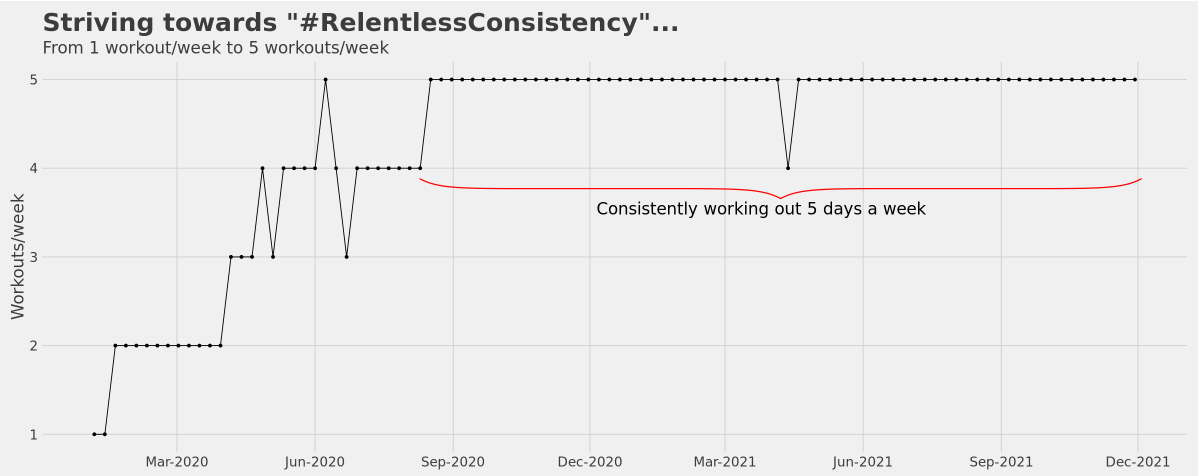
\includegraphics{pictures/relentless.png}
\caption{Relentless consistency}
\end{figure}

\hypertarget{the-choice-between-work-and-workouts-is-a-false-binary}{%
\section{The choice between ``work'' and ``workouts'' is a false binary}\label{the-choice-between-work-and-workouts-is-a-false-binary}}

When I started working out, the priority order between work and workouts was very clear, in fact it was not even a question, it was always work first and workout later. Said another way, if there was a choice between workout and what pays for the workout then I would always choose what pays for the workout i.e.~my work. I realize now that this is a false binary.

I have had several instances where I rescheduled my workouts just because there was a crisis at work, a meeting that was too close to my workout time (allowing very little time to do some pre-meeting prep work) or even for some not so pressing reasons, so much so that it was more of an excuse rather than an actual requirement. As time passed, I realized that the benefits of the workouts translated directly into my work, my focus improved, I became more efficient because I had this thing in my life that I did not want to short shrift so I had to finish the work in the time I had, and in general I just felt good after a workout.

The number of times I have felt ``oh, maybe I would have been better off not working out and taking care of this other distraction-of-the-day'' is exactly zero. Whereas the number of times I have felt ``oh, I am so glad that I did not negotiate with myself and just did the workout'' is too many to count. Life happens, competing priorities exist all the time, we just need to know that workout is also a high priority.

As I moved my workouts to the morning before the start of my workday, the benefits became much more tangible. I could feel it during my meetings that I was much more engaged and just had a sense of ``oh, I got this'' (maybe my brain was thinking I just deadlifted 300 pounds, compared to that this is easy). It has come to a point now that I feel, how will I even operate if I do not start my workday riding a post-workout high? Workouts do result in better performance at work, in my experience at least. Someone said to me at work the other day, ``Amit, you have a lot of responsibility on your shoulders'', and my response right off the bat was ``yes, that is why I work out regularly to broaden those shoulders\ldots{}'' and that brought a smile to everyone's face. While this was a comment made in jest, but to me it is a true statement, my workouts do indeed provide the fuel for work (and vice-versa, after all my work does pay the bill for my workouts).

If any CEOs out there are reading this book, I implore you to incentivize workouts and an 8-hour sleep schedule for your employees, the benefits to the bottom line are real.

\hypertarget{the-right-time-to-start-was-yesterday-but-the-best-time-to-start-is-today}{%
\section{The right time to start was yesterday, but the best time to start is today!}\label{the-right-time-to-start-was-yesterday-but-the-best-time-to-start-is-today}}

Do not procrastinate, look ahead and start today. We often procrastinate to start. Often it is because of a thought in our head that says, ``it is probably too late, you should have started yesterday or better still, 10 years ago''. While it is probably true that an early start would have helped, but that should not stop us from starting now and improving the future, should it?

An advantage we have now is the realization that it was the right thing to do, whether it was taking charge of our health by starting on a fitness routine, switching jobs for that non-linear growth or anything else. Your unique life circumstance is now telling you to begin, take charge and start now, yesterday is gone and the future is yet to come.

I did not set foot in a gym until I was 41 years old and now almost 2 years later, I workout 5 days a week. I am leaner and stronger at 42 than I was at 22. \textbf{The best time to start is today!}

\hypertarget{read-read-read}{%
\section{Read, read, read\ldots{}}\label{read-read-read}}

As they say, one good habit begets another, out of my interest to learn more about nutrition and fitness and initiated but a birthday gift from a friend I started reading books again. Unlike in the past, when I would buy books out of a genuine intent to read but then put them down after reading a few chapters, this time I followed through. After all, I have been working out consistently five times a week and could surely put the same power to good use elsewhere as well (at least that is what I told myself)! I have tried to weave reading into my morning routine, could be just a few pages, a few times a week but no week should go by with me not reading anything. I try to reserve 10 minutes in the morning, right before I go to the gym, for reading a book along with a good coffee.

Here is a picture from one of the more perfect mornings, made up of a good book, a good cup of coffee and a breathtaking view. Taken at an Airbnb in Smoky Mountains, Tennessee, in the summer of 2021.

\begin{figure}
\centering

\includegraphics{pictures/smoky_morning.png}
\caption{Morning Read}
\end{figure}

I read almost 12 books this year, all non-fiction, all related to health \& fitness or motivation and personal growth. Reading is now a part of my life priorities almost as much as fitness is and the more I read and enrich my mind the more I realize how much there is that I don't know. I would attribute rediscovering reading also to the gains I made while working out, it was as if the workouts flipped a switch in my head and I realized that just like I could find time for working out, I could also find time for reading (which meant less time for television). Truly, one good habit begets another.

At the start of the year I thought I should read at least a book a month, turned out it was more ambitious a target than I initially thought. The books I read in 2021 can be divided into three categories:

\begin{itemize}
\item
  Perspective on how we can make life more productive and rewarding: Atomic Habits, The infinite game, Think Again, Deep Work
\item
  Health \& Fitness: Why we sleep, Eat like the animals, Breath: the new science of a lost art, Breathing for warriors, The biology of belief
\item
  Personal stories for inspiration: Finding Ultra, Can't hurt me, The code breaker
\end{itemize}

I gained so much from reading \href{https://www.instagram.com/p/CW1yGyBsvLk/}{these books}.

\hypertarget{what-about-supplements}{%
\section{What about supplements?}\label{what-about-supplements}}

We did take supplements for micro-nutrients (vitamins and minerals). To be clear, the intention was not to take supplements for muscle building but for general health, more like an insurance against missing out key micro-nutrients from the food. Even with the previous protein-based diet program that I followed earlier there was a recommendation for different vitamin and minerals supplements so when we started exercising more, the topics of supplements came up organically. We discussed with our trainer and as I started reading more and more, I got more convinced that we should take some micro-nutrient supplements to augment what we were eating. I did my own research, which is a fancy way of saying I looked up supplements and their effects on \url{labdoor.com} and \url{examine.com} and discussed with my trainer as to which supplements were required and which brands had ingredients which were minimal and safe.

Here is my list:

\begin{itemize}
\tightlist
\item
  Vitamin D
\item
  Vitamin C
\item
  Zinc
\item
  Multi Vitamins
\item
  Fish Oil
\item
  Probiotics
\item
  Amino Acids
\item
  Creatine Monohydrate
\end{itemize}

Did not start taking these supplements from day 1, this happened over a 6-month period. \textbf{Do not start any supplements without first consulting with your doctor.}

\hypertarget{small-knobs-big-knobs}{%
\section{Small knobs \& big knobs}\label{small-knobs-big-knobs}}

Exercise and nutrition are the big knobs by which we can control weight and general health. As we progressed through our journey, we realized that there are small knobs as well which are needed to fine tune the body's response during the proverbial last mile. Losing first few pounds is easy, as most people would say, maybe even losing the first 5 pounds is easy, losing the last 5 pounds is insanely hard. That is where the small knobs become extremely important. The small knobs are

\begin{itemize}
\item
  Sleep: I have noticed this several times, not having a good sleep shows up unfavorably on the weighing scale the next morning. With my level of exercise now my body demands a good 7-hour sleep.
\item
  Making sure you are not taking less calories than what your body needs: if the body is not getting enough calories it will fight to keep whatever fat it has and therefore weight loss will become difficult. I have certainly experienced this.
\item
  Stress: we all live extremely busy lives, the demands of work, family and social engagements does cause stress and too much stress is bad for weight loss in the same way it is bad for anything else.
\end{itemize}

\hypertarget{for-the-love-of-charts}{%
\section{For the love of charts}\label{for-the-love-of-charts}}

Here are some more charts that I could not fit anywhere else.

\hypertarget{how-many-days-did-it-take-to-lose-every-single-pound}{%
\subsection{How many days did it take to lose every single pound?}\label{how-many-days-did-it-take-to-lose-every-single-pound}}

Sometimes we get anxious, about being stuck at a specific weight or oscillating within a few pounds. As enough data got collected, we could see empirically how many days we spent at each weight level so that before we start getting anxious we know if we really need to or is it still within an observed range.

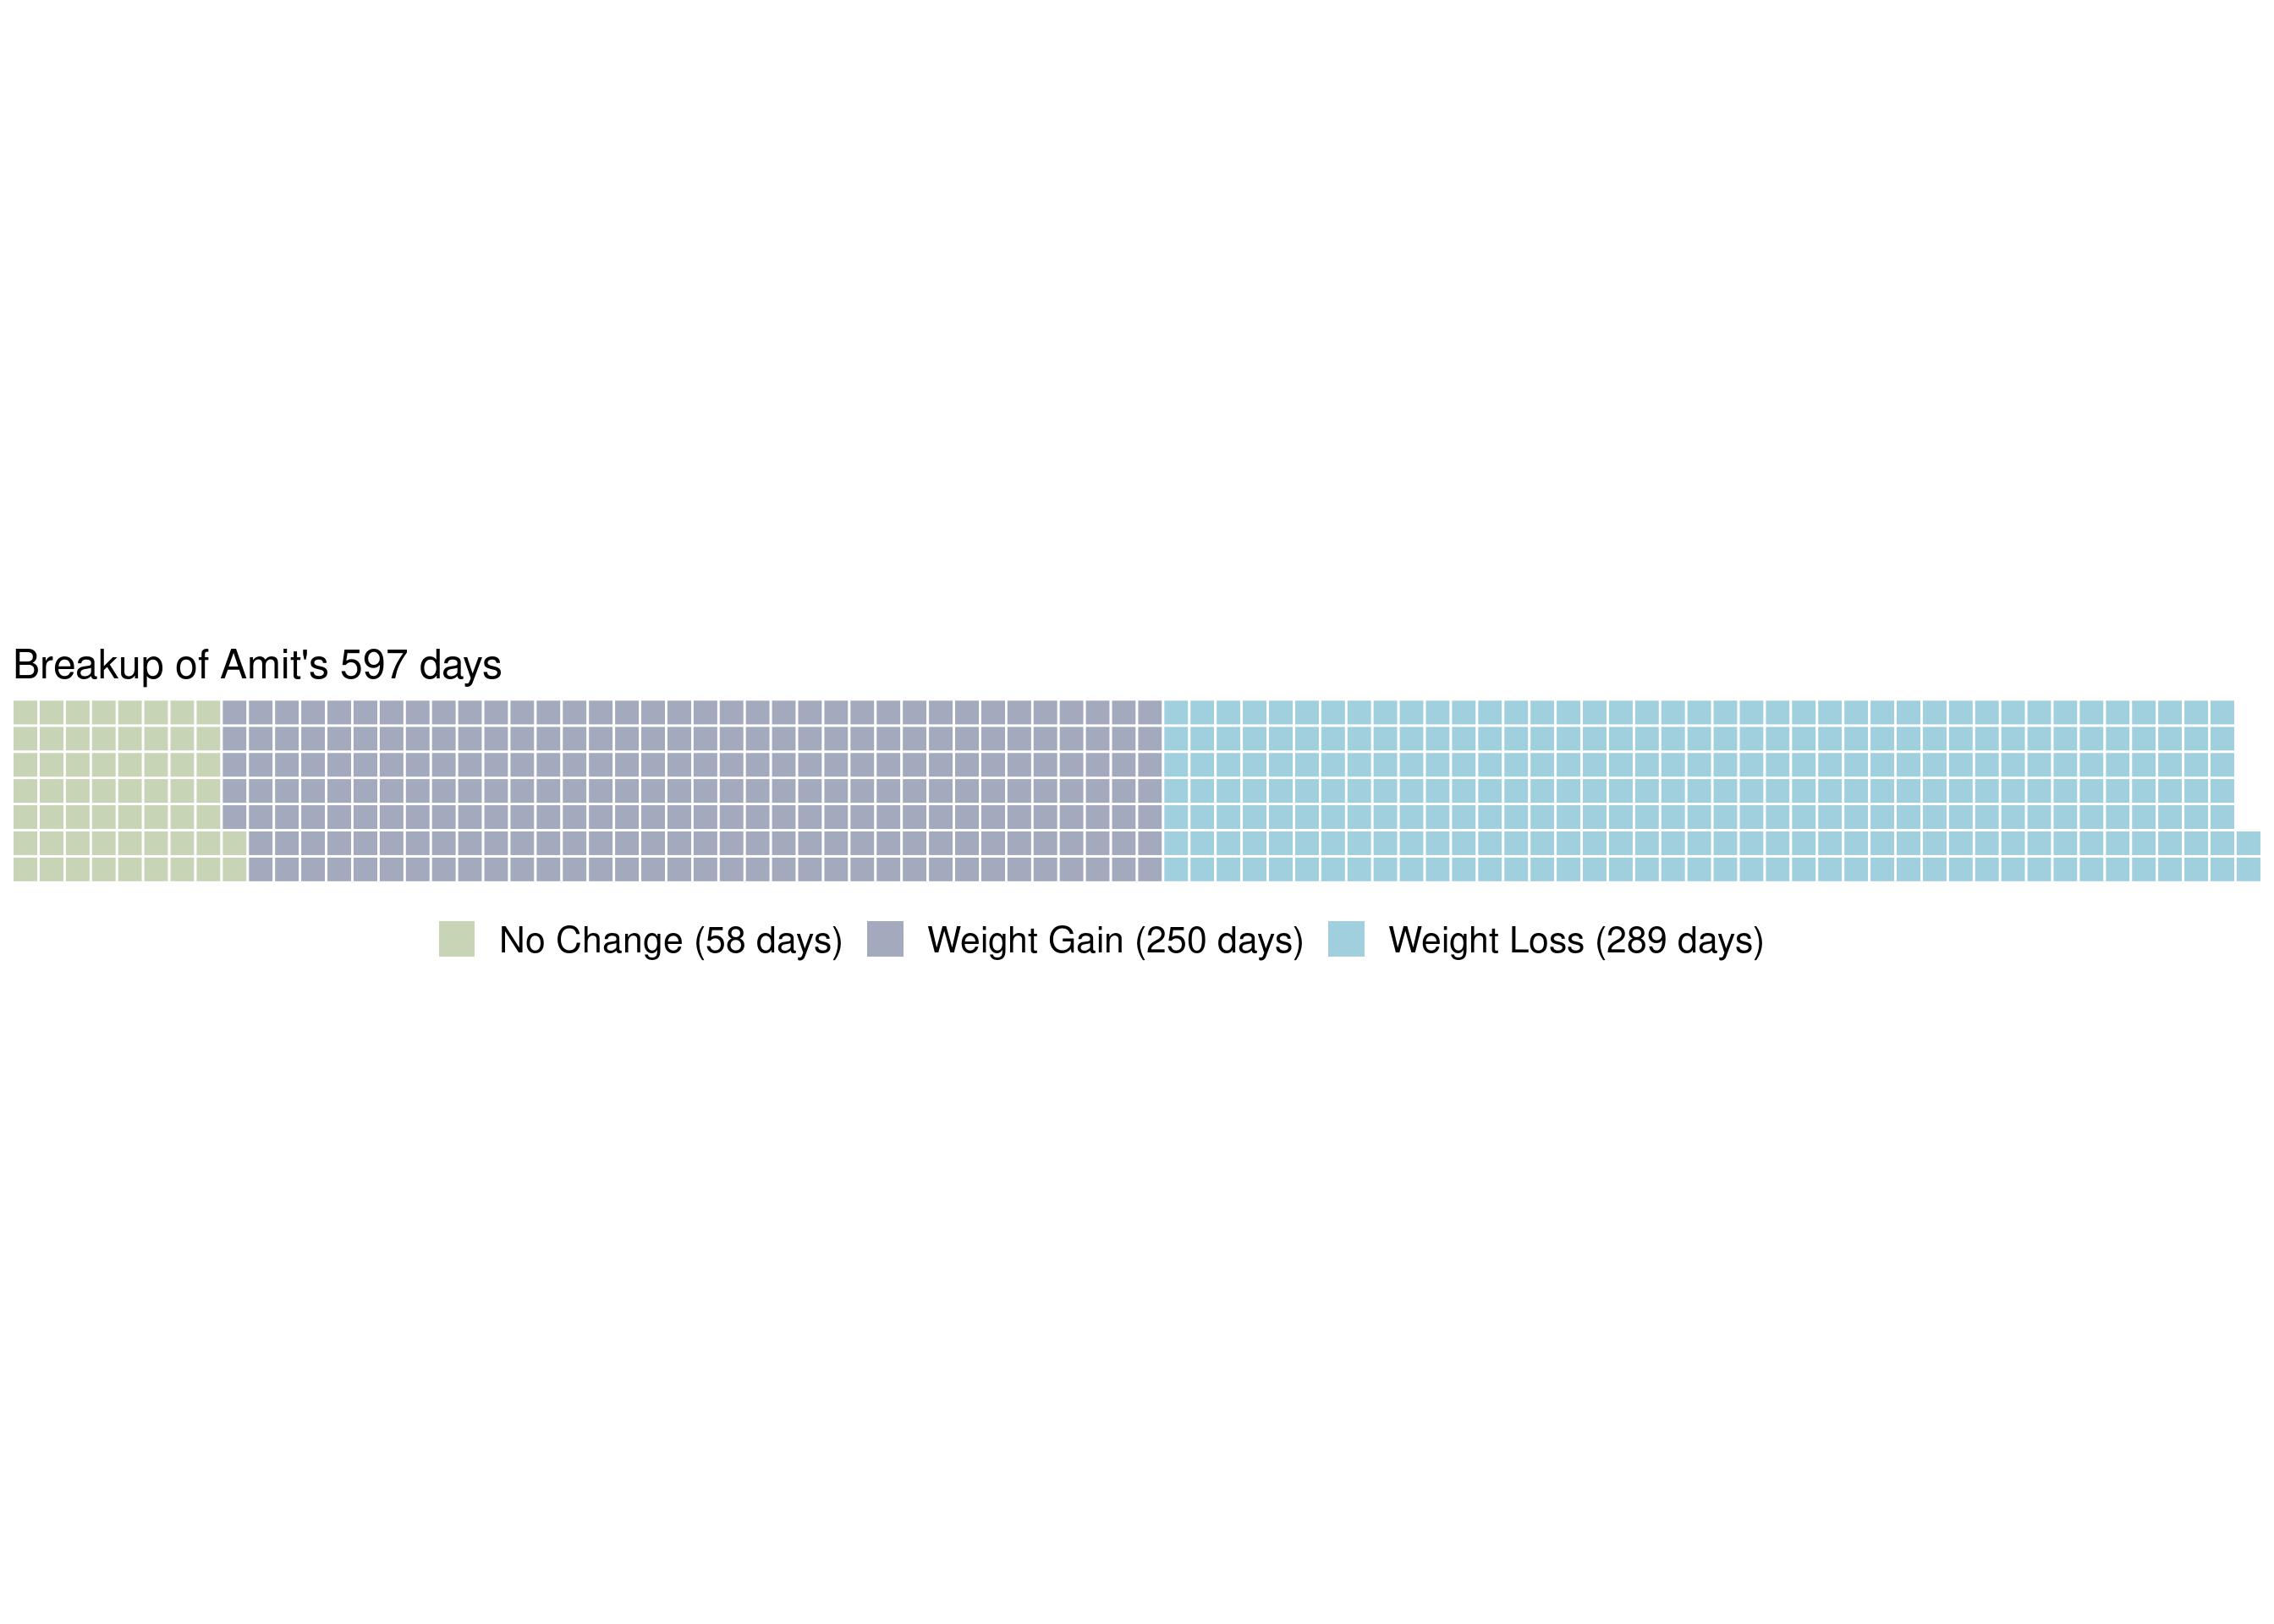
\includegraphics{bookdownproj_files/figure-latex/unnamed-chunk-25-1.pdf}

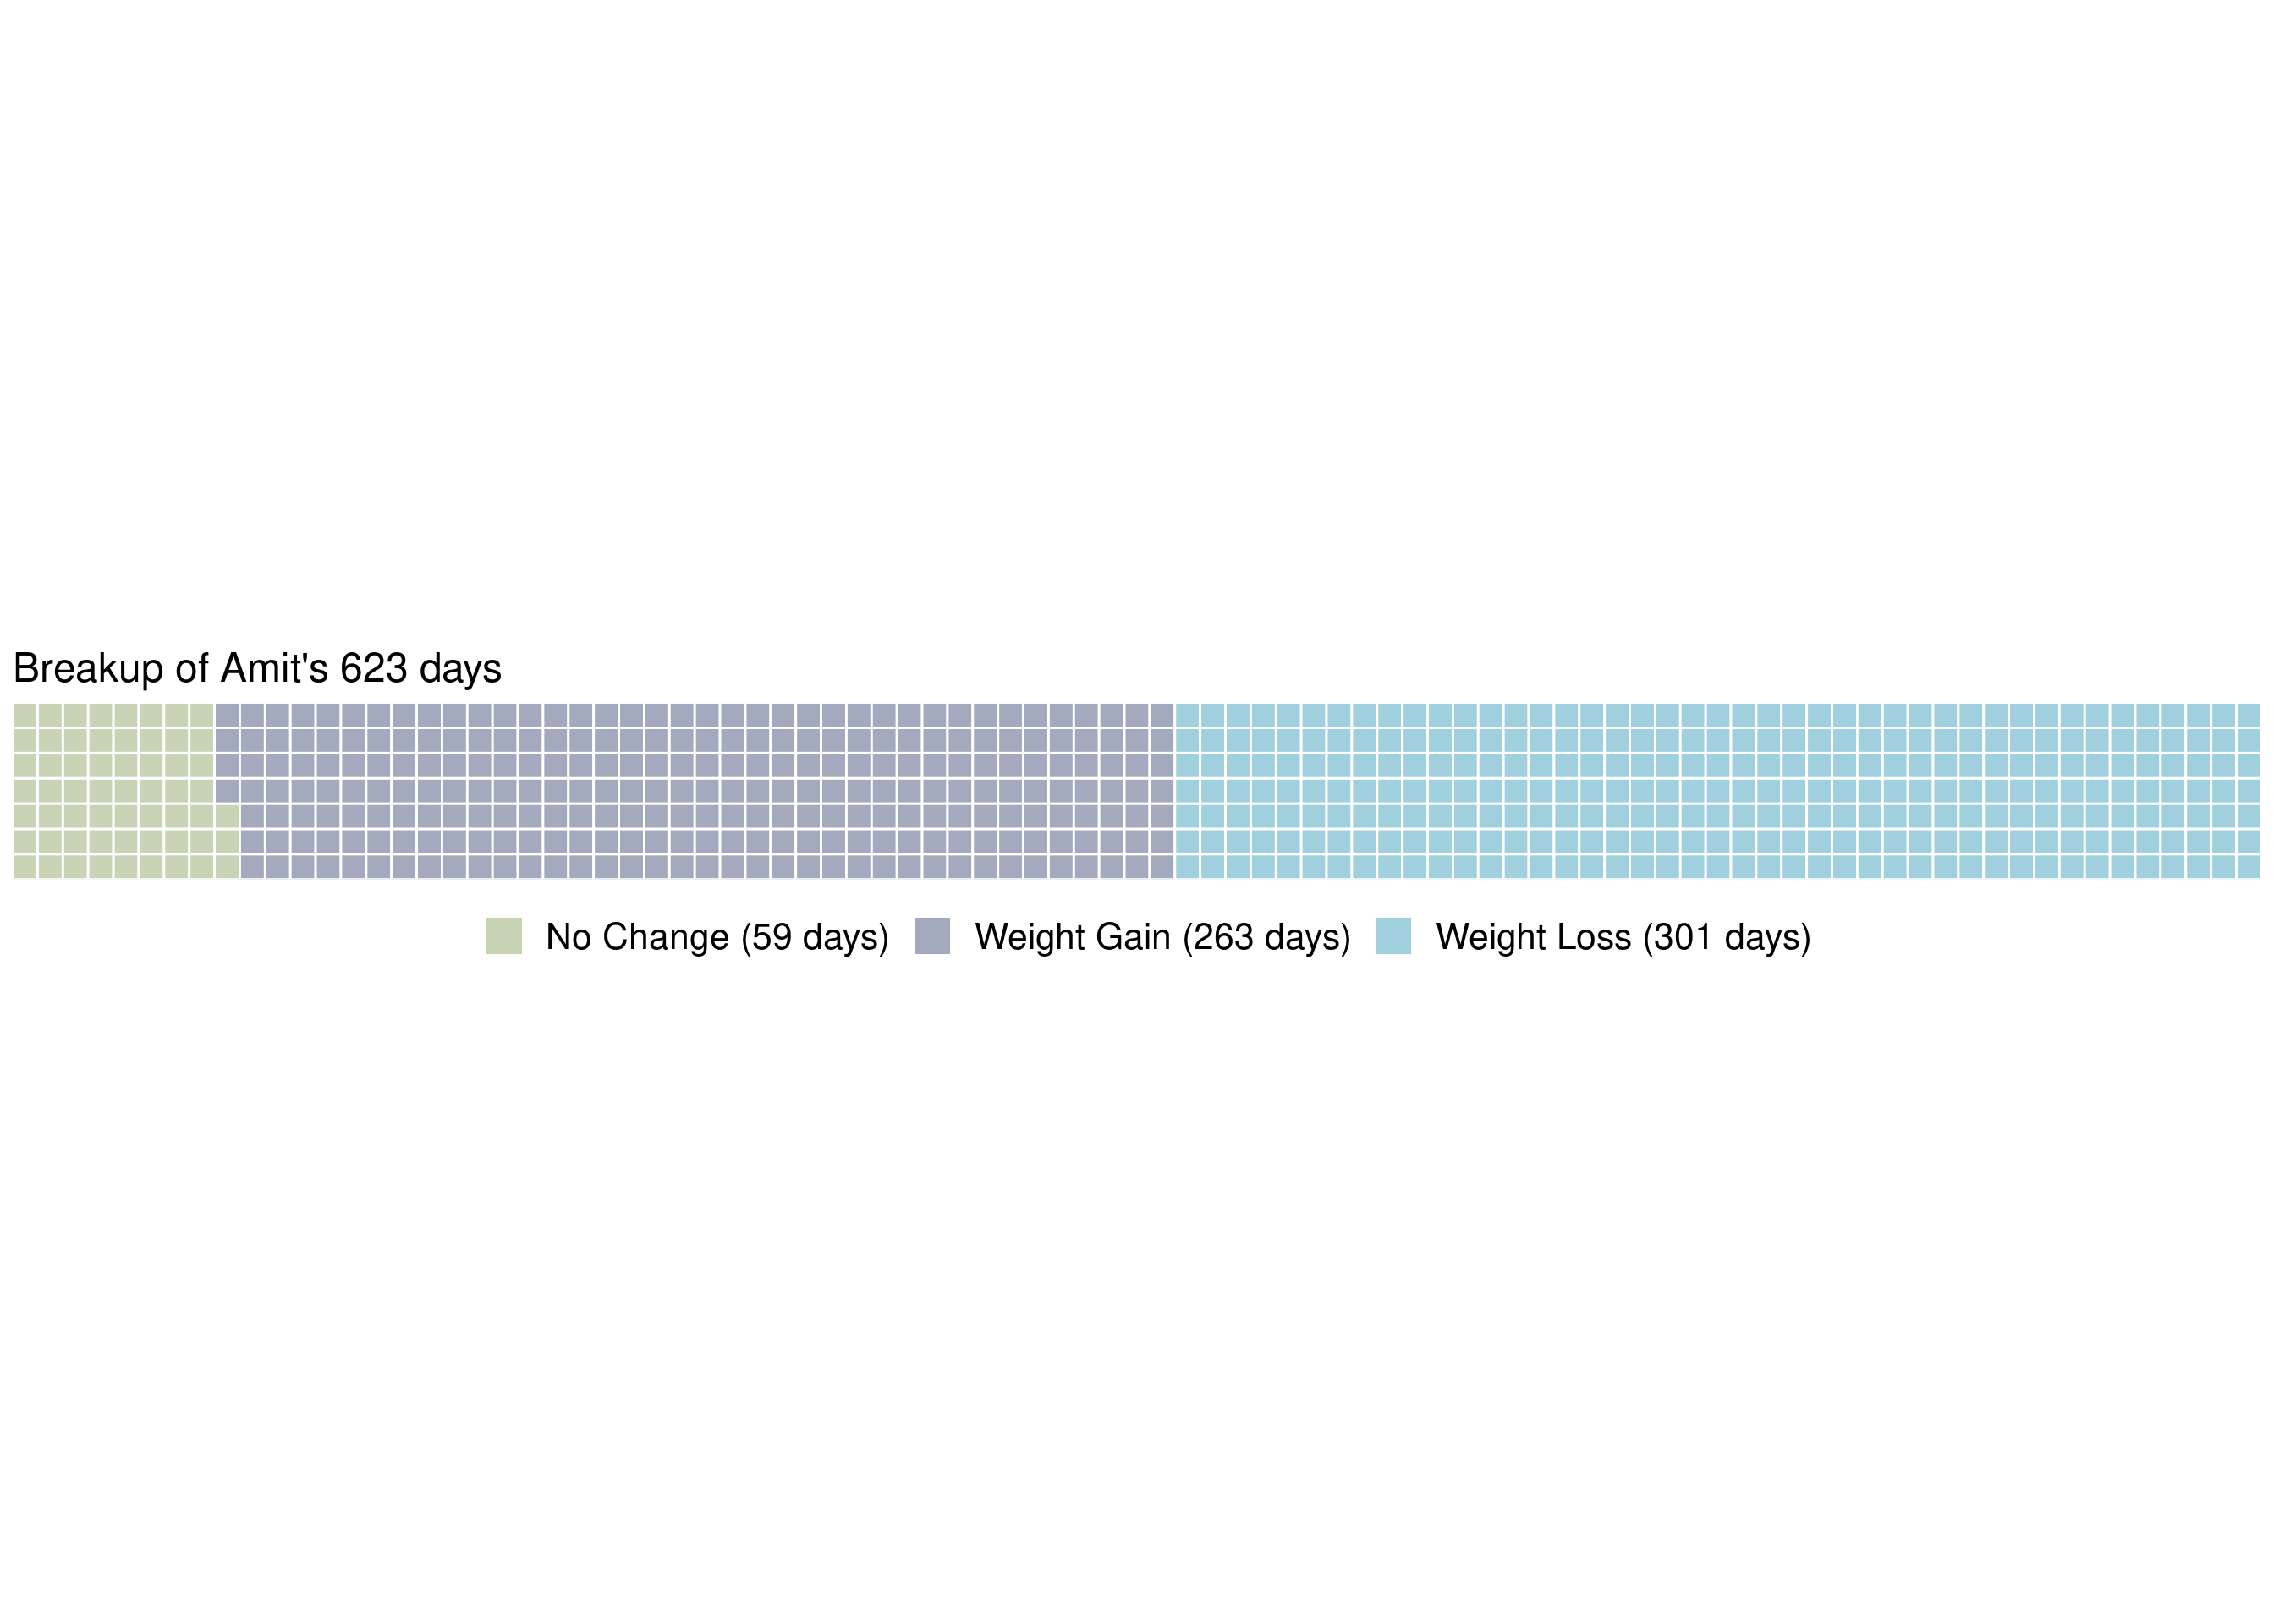
\includegraphics{bookdownproj_files/figure-latex/unnamed-chunk-26-1.pdf}

\hypertarget{breakup-of-the-days}{%
\section{Breakup of the days}\label{breakup-of-the-days}}

We know we lost weight on more days than we gained weight (otherwise this book would not exist), but a good visualization is always welcome.

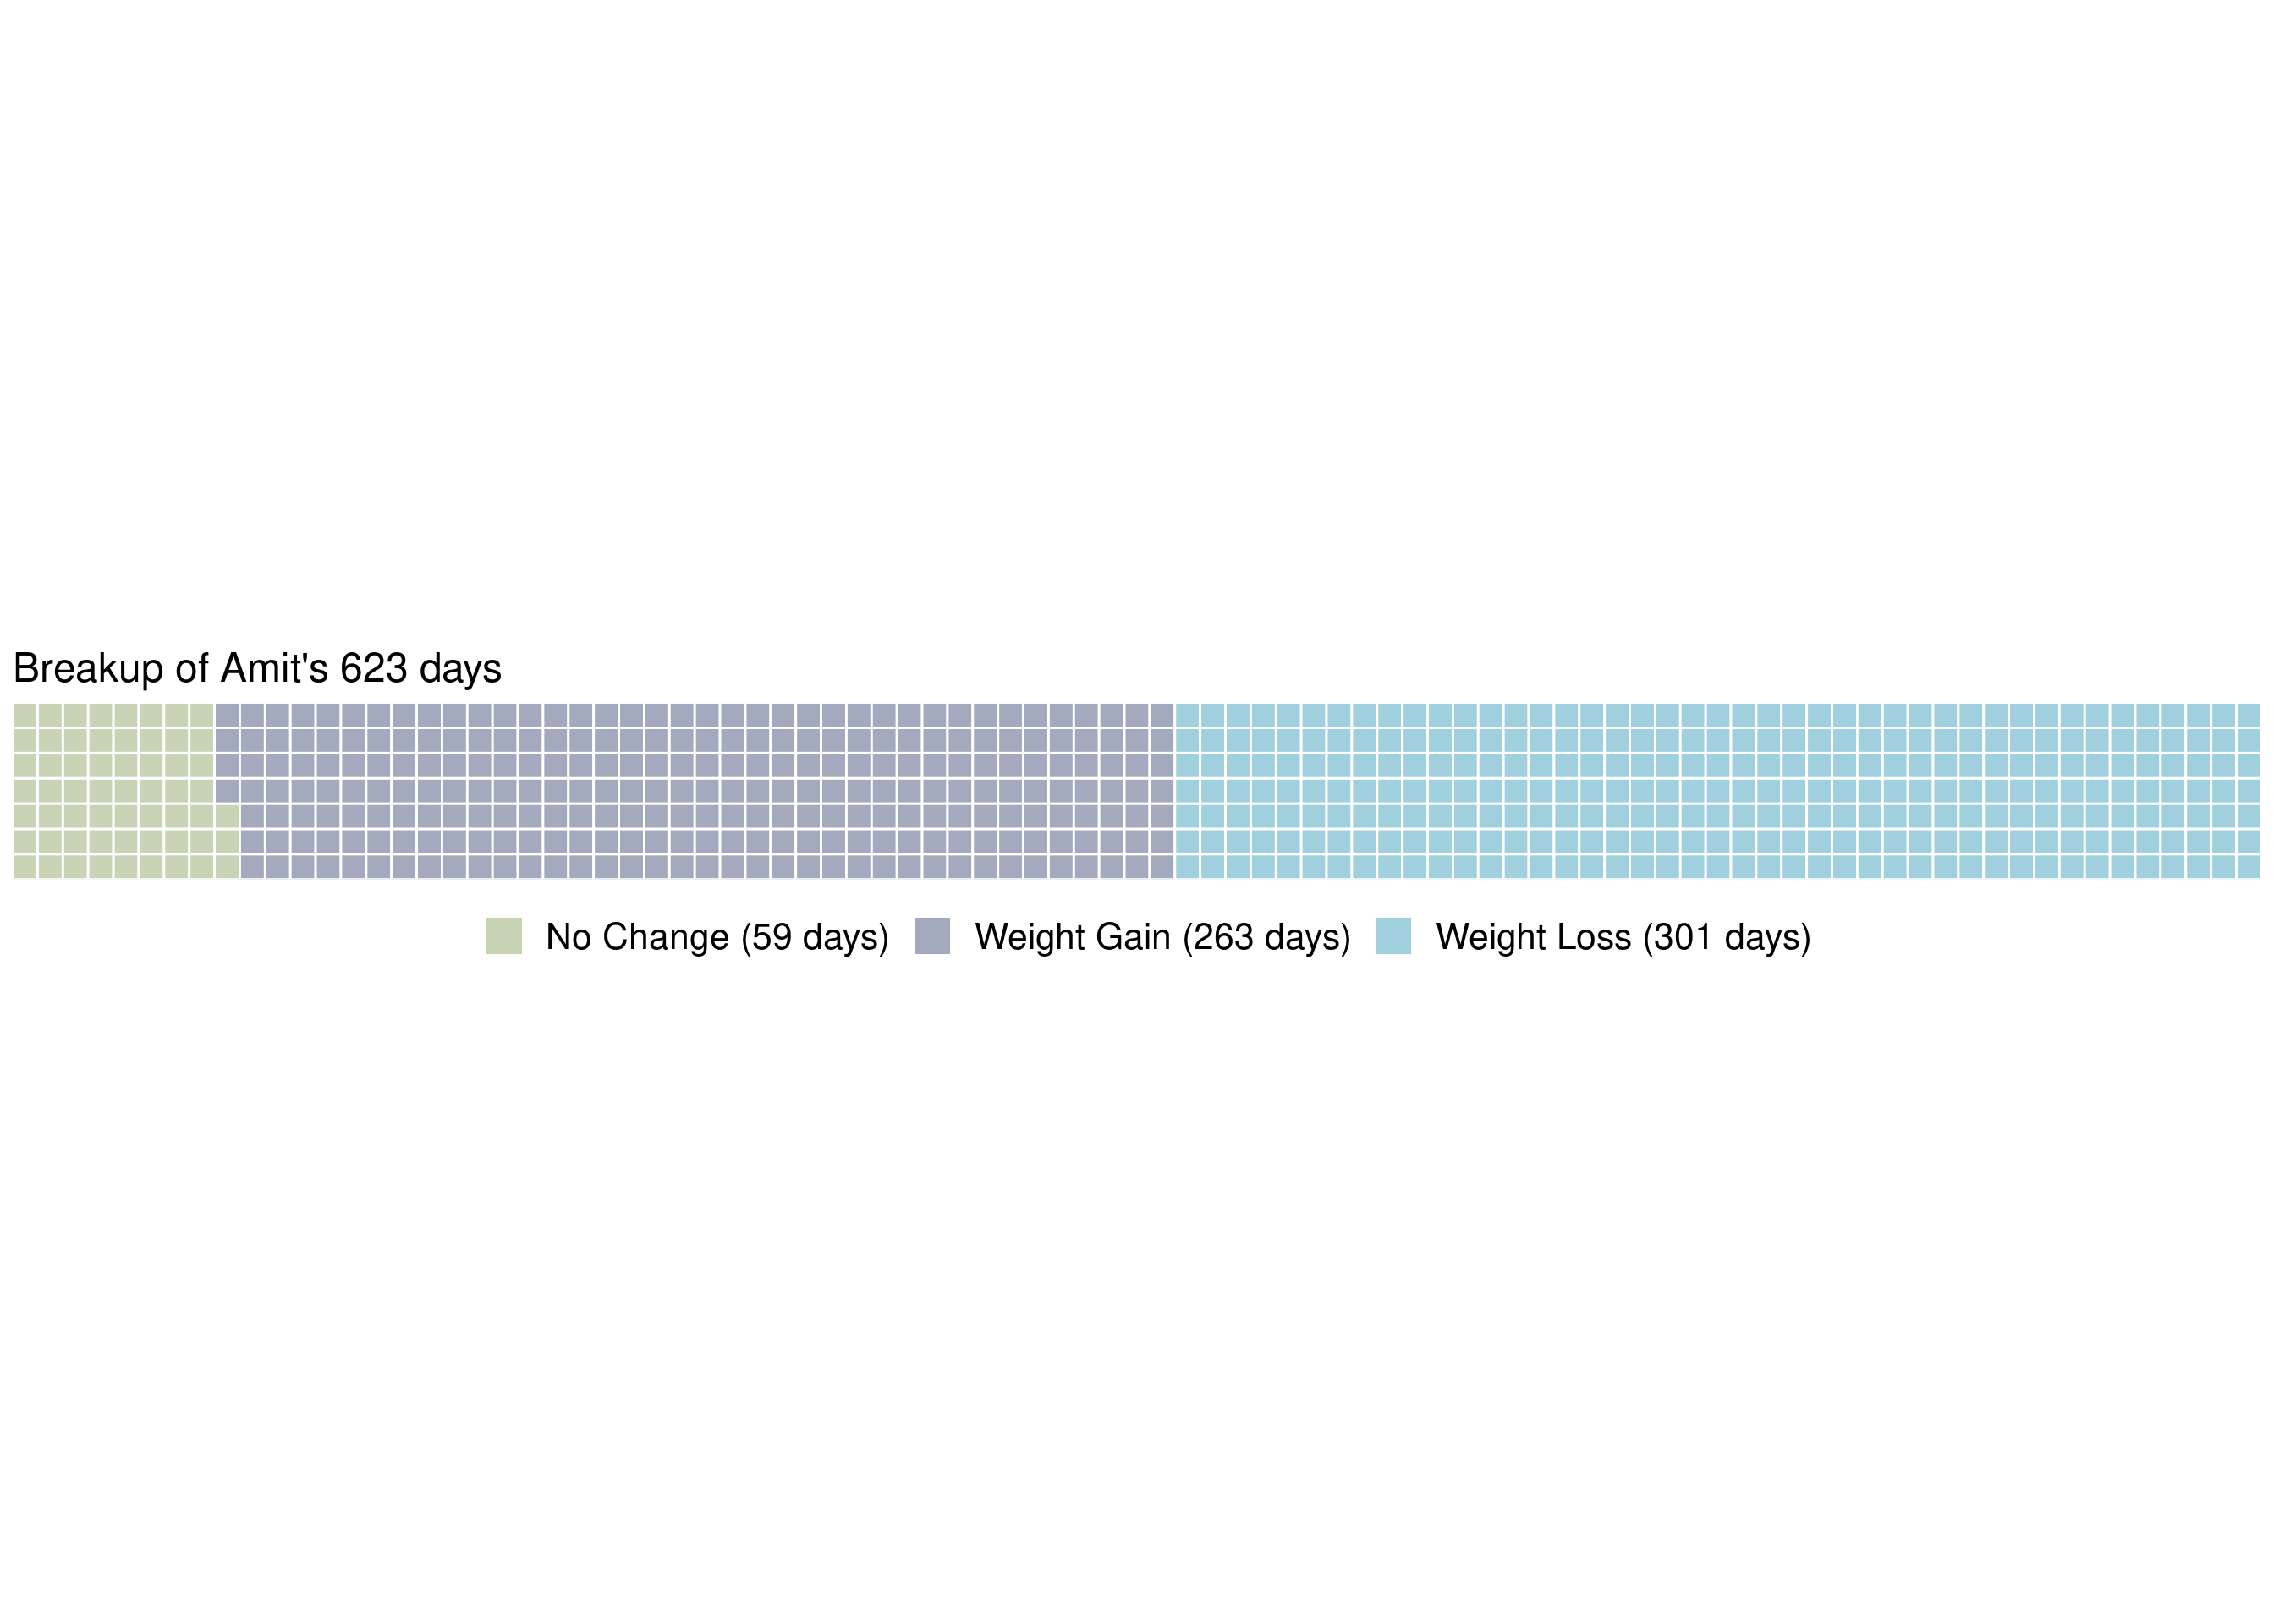
\includegraphics{bookdownproj_files/figure-latex/unnamed-chunk-27-1.pdf} 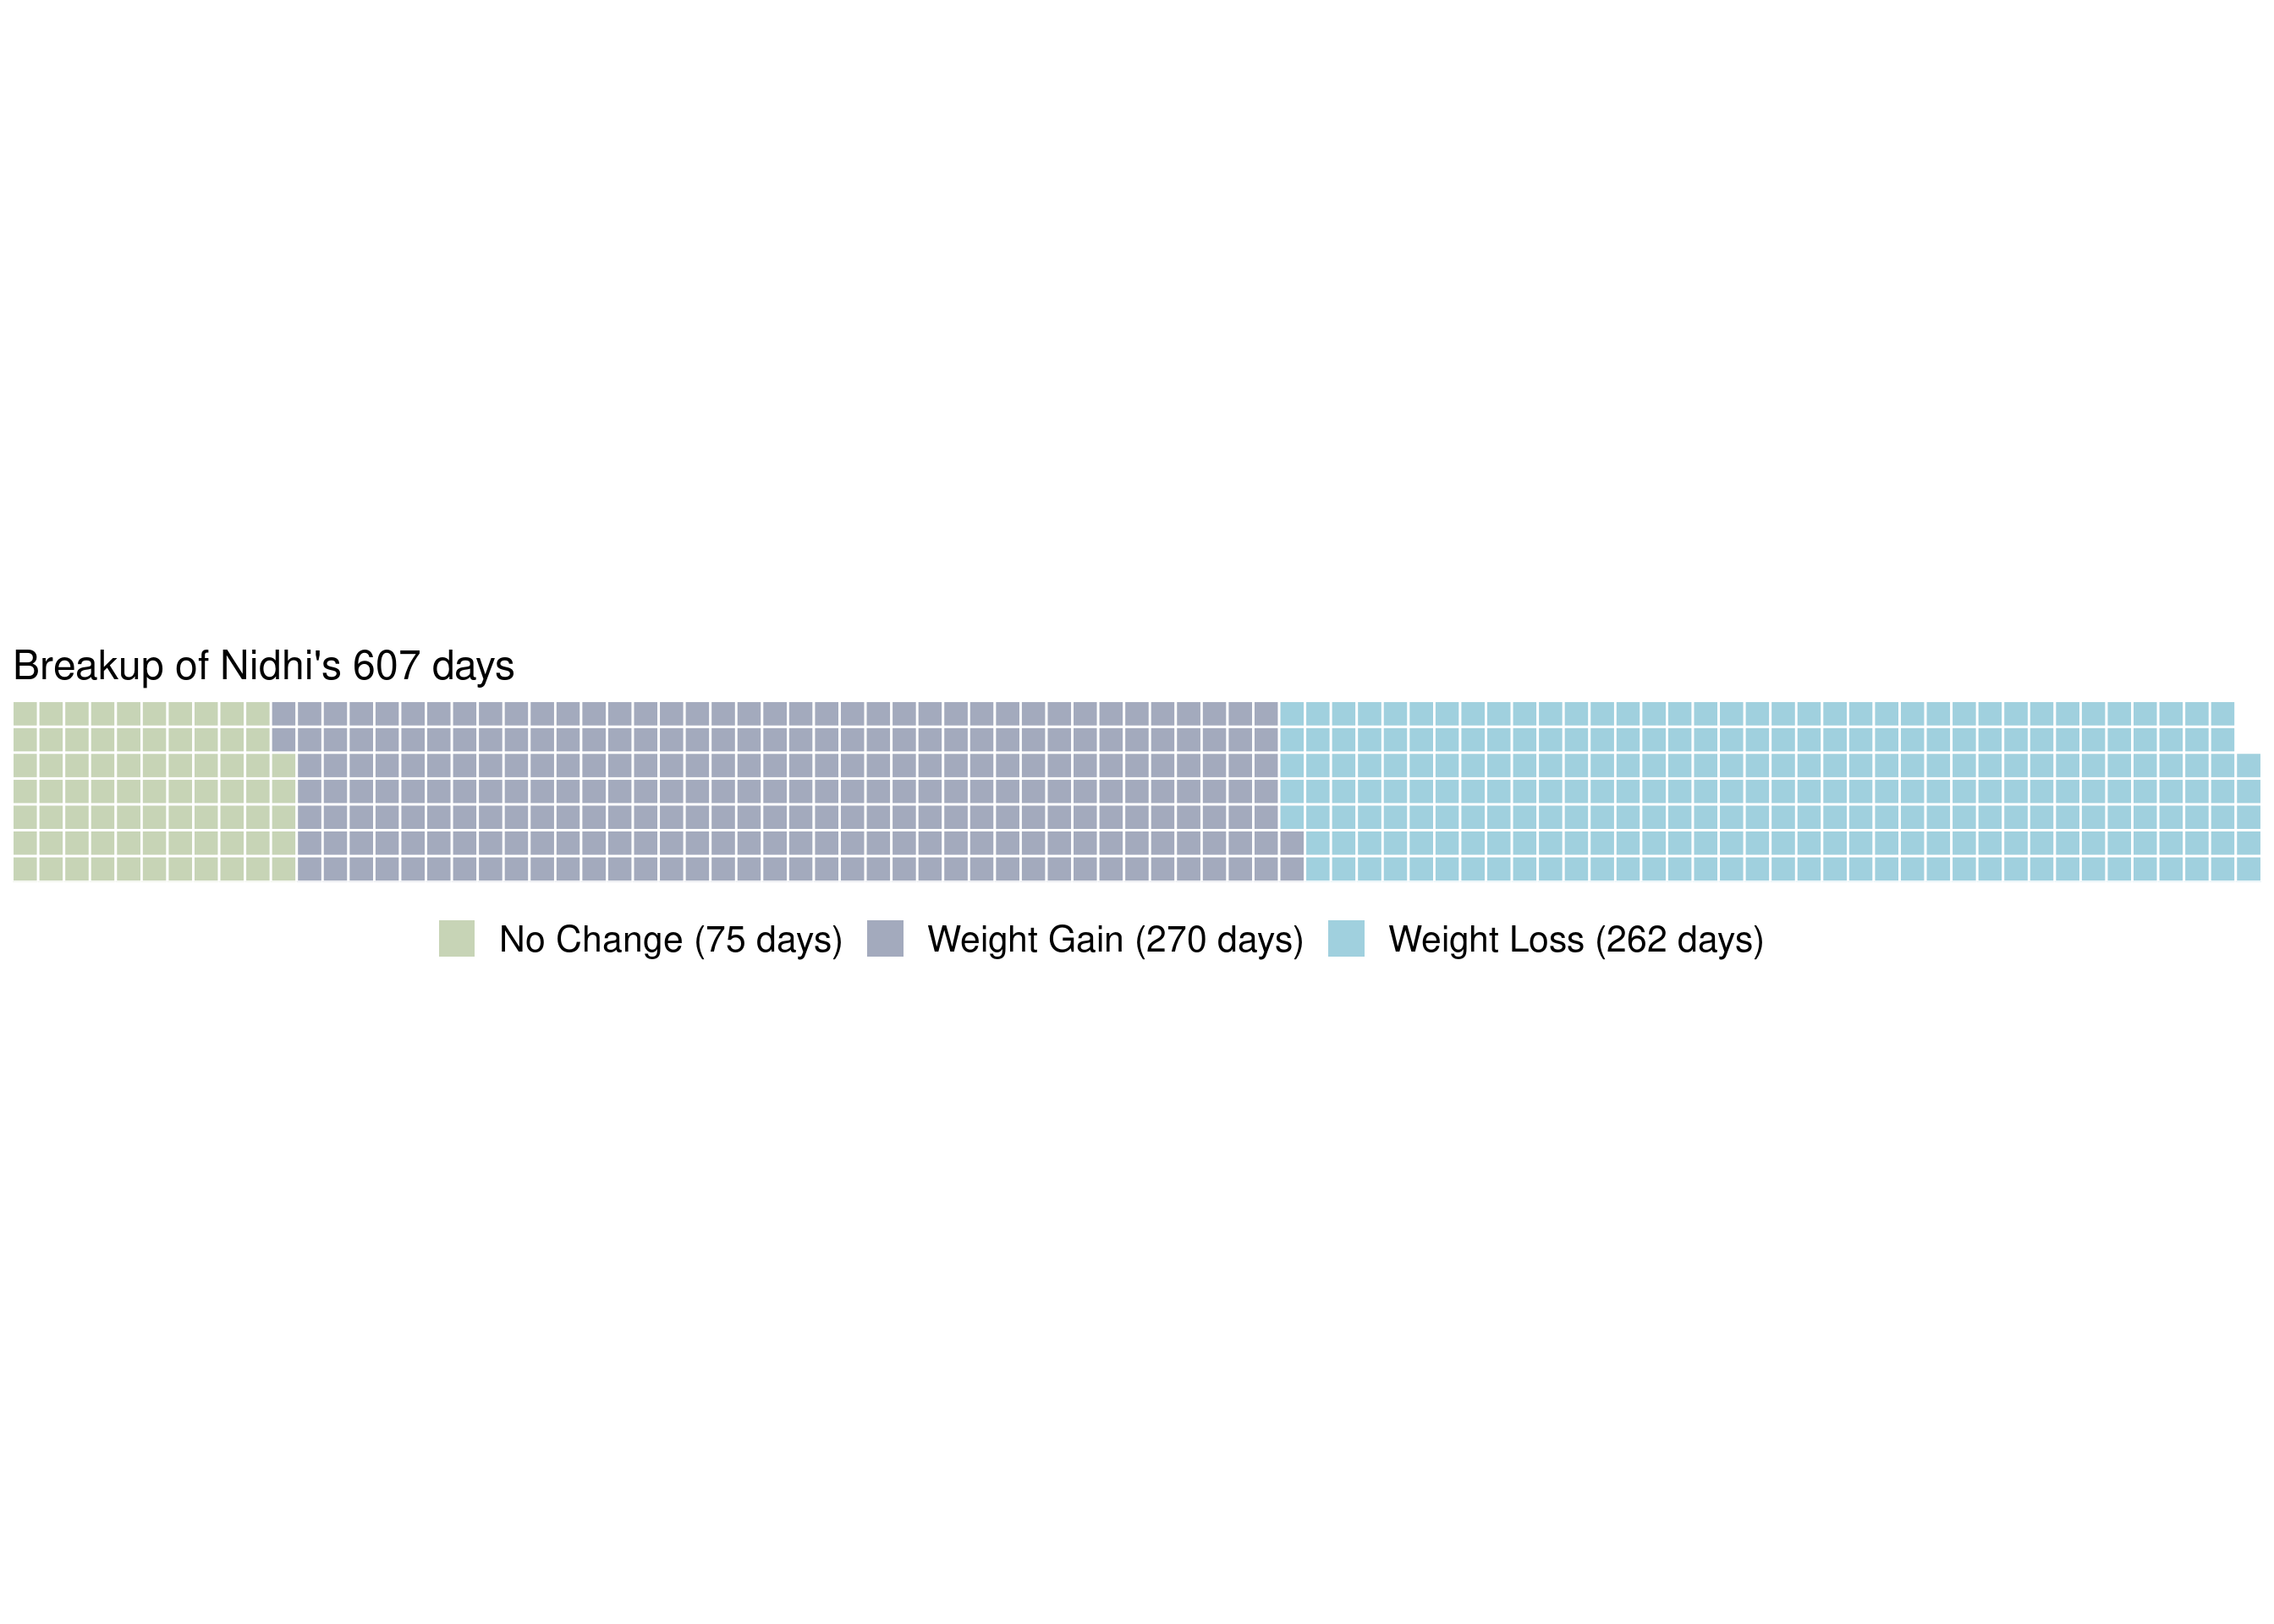
\includegraphics{bookdownproj_files/figure-latex/unnamed-chunk-27-2.pdf}

\hypertarget{chapter-10-at-a-glance}{%
\section{Chapter 10: At a glance}\label{chapter-10-at-a-glance}}

\begin{center}\rule{0.5\linewidth}{0.5pt}\end{center}

\begin{enumerate}
\def\labelenumi{\arabic{enumi}.}
\item
  The benefits of consistent workouts go far beyond benefits to the body, they transcend into better habits all around, better cognition and a better life.
\item
  There are no quick fixes, no silver bullet, no one diet to fix it all. Consistency with a relatively clean eating regimen (avoid processed foods), regular workouts and good sleep is the answer.
\end{enumerate}

\hypertarget{recipes}{%
\chapter{Recipes}\label{recipes}}

One of the most frequent feedback that we got on the first edition was: ``how can we try some of the delicious foods that we see in the book?''. While a lot of our friends have since been to our home to try some of the salads but for those whom we have not yet had the pleasure of hosting, here a few recipes that you can try out. Goes without saying, I am just the scribe here, this is all (like a lot of good things) credit to Nidhi.

\hypertarget{seasame-garlic-tofu}{%
\section{Seasame Garlic Tofu}\label{seasame-garlic-tofu}}


\includegraphics{pictures/Seasame-garlic-tofu.png}\\
Ready in 20 minutes. Serves 4 people

\hypertarget{ingredients}{%
\subsection{Ingredients}\label{ingredients}}

\begin{enumerate}
\def\labelenumi{\arabic{enumi}.}
\tightlist
\item
  Tofu 28 oz
\item
  Sesame oil 2 tbsp
\item
  Arrowroot Starch 2 tsp
\item
  Spring onions 5 to 6 (sliced with white and greens separated)
\item
  Garlic 2 flakes grated
\item
  Sesame seeds for garnish 1/2 tsp
\end{enumerate}

\hypertarget{preparation}{%
\subsection{Preparation}\label{preparation}}

Pre-preps for tofu:

\begin{enumerate}
\def\labelenumi{\arabic{enumi}.}
\item
  This recipe tastes best with the crispy texture of tofu. To get the crispy effect tofu must be dried from outside.
\item
  Tofu comes submerged in water, drain the water in the sink and wash and pat dry the tofu. Then place it on a flat base with a slight angle (I did it in my kitchen sink only), sandwiched between kitchen towels and put some weight on the top of the tofu. Make sure the weight is not so much that the tofu gets crushed, however, just enough to squeeze the extra water from tofu. I used an iron skillet as the weight.
  If possible, leave it like this before you go to the office and let it stay for a few hours. Or speed up the process by changing the kitchen towels frequently. This will take at-least 30 minutes.
\item
  Cut the tofu in about 1-inch cubes. Add the cut tofu in a platter and sprinkle cornflour. Toss the cubes to evenly coat with cornflour.
\end{enumerate}

Cooking instructions:

\begin{enumerate}
\def\labelenumi{\arabic{enumi}.}
\item
  Take an iron skillet and heat it before adding oil. Once hot, add oil, place the prepared tofu, do not overlap.
\item
  Do not turn till one side is completely done, brown all the edges. This will take around 15 minutes. (I had to do two rounds as all the tofu could not fit in one round).
\item
  In a bowl add all the ingredients of sauce and whisk them together. Once all sides of all tofu cubes are browned, add garlic in the skillet and saute for 30 seconds.
\item
  Then add all part white and half part greens of spring onion, saute for another 30 seconds. And pour the sauce on top.
\item
  Quickly stir and evenly quote all the tofu with the sauce. You need to cook till you get the shiny looking texture. That means the cornstarch is cooked completely. This will take 3-4 minutes.
\item
  Transfer them in a serving dish garnish with spring onion greens and sesame seeds.
\end{enumerate}

\hypertarget{preparing-gravy}{%
\subsubsection{Preparing Gravy:}\label{preparing-gravy}}

\begin{enumerate}
\def\labelenumi{\arabic{enumi}.}
\tightlist
\item
  In the same skillet add some water and some chili garlic sauce. Mix it well and take out all the sauce left behind in the skillet. This will make a thin gravy which I used to drizzle on my plated sesame tofu and stir-fried broccoli.
\end{enumerate}

Tip:
Arrowroot Starch can be replaced with cornstarch. To make it a complete meal for my kids, I added some rice with a gravy drizzle we ate with Cauliflower rice.

\hypertarget{egg-wraps}{%
\section{Egg Wraps}\label{egg-wraps}}

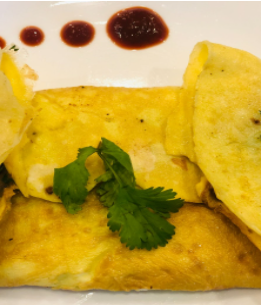
\includegraphics{pictures/egg-wraps.png}\\
Ready in 15 Mins. Serves 1.

\hypertarget{ingredients-1}{%
\subsection{Ingredients}\label{ingredients-1}}

\begin{enumerate}
\def\labelenumi{\arabic{enumi}.}
\tightlist
\item
  Eggs whole 2
\item
  Mushroom 1/4 cup diced
\item
  Green peppers 1/4 cup diced
\item
  Onions 1/4 cup diced
\item
  Coriander 1/4 cup diced
\item
  Green chili finely chopped (optional)
\item
  Ham diced 1 tbsp
\item
  Cajun Spice 1/8 tsp (optional)
\item
  Salt 1/4 tsp
\item
  Black pepper powder 1 pinch
\item
  Ginger powder 1 pinch
\item
  Olive oil 1/2 tsp
\end{enumerate}

\hypertarget{preparation-1}{%
\subsection{Preparation}\label{preparation-1}}

\begin{enumerate}
\def\labelenumi{\arabic{enumi}.}
\item
  In a bowl crack open the eggs and beat them well add 2 pinches of salt.
\item
  Heat a big flat pan, spray some oil and spread the egg and let it cook, when one side is cooked flip and both sides. Do not make it crisp, it should be easy to fold.
\item
  While the eggs are cooking at the same time in a separate pan add olive oil, all the vegetables and all the spices. You need to cook till mushrooms reduce their size and start getting roasted.
\item
  Now place the cooked vegetables in the center of the egg and wrap the egg around it as shown in the picture.
\item
  Serve it hot with sriracha sauce.
\end{enumerate}

\hypertarget{spinach-soup}{%
\section{Spinach Soup}\label{spinach-soup}}

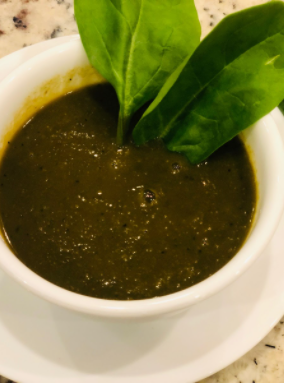
\includegraphics{pictures/spinach-soup.png}\\
Ready in 20 minutes. Serves 3 people.

\hypertarget{ingredients-2}{%
\subsection{Ingredients}\label{ingredients-2}}

\begin{enumerate}
\def\labelenumi{\arabic{enumi}.}
\item
  Spinach 1 bunch cleaned and roughly chopped
\item
  Tomato 1 roughly chopped
\item
  Carrot 1 small
\item
  Zucchini 1 cup (in my case I used the scrapes left from zucchini boats)
\item
  Green chili 2 (optional)
\item
  Ginger root 1/4 inch
\item
  Salt 1 tsp (or to taste)
\item
  Black pepper powder 1/4 tsp
\item
  3 cups of water
\end{enumerate}

\hypertarget{preparation-2}{%
\subsection{Preparation}\label{preparation-2}}

\begin{enumerate}
\def\labelenumi{\arabic{enumi}.}
\item
  Add all the vegetables with salt and 2 cups of water in a pressure cooker and cook up to two whistles.
\item
  Leave it for 10-15 minutes for the pressure to subside by itself.
\item
  Blend them in a blender and pour it in a pot. Now use 1 cup of water to rinse the blender and add to the pot, boil for 2 minutes. Add pepper powder, mix and taste to adjust salt.
\item
  Serve it hot.
\end{enumerate}

Tip:
Add butter before eating, Butter will make the soup's texture creamier.

\hypertarget{egg-drop-soup}{%
\section{Egg Drop Soup}\label{egg-drop-soup}}

\begin{figure}
\centering
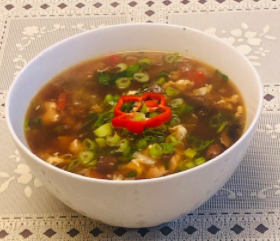
\includegraphics{pictures/egg-drop-soup.png}
\caption{Egg Drop Soup}
\end{figure}

Ready in 30 minutes. Serves 4 people.

\hypertarget{ingredients-3}{%
\subsection{Ingredients}\label{ingredients-3}}

\begin{enumerate}
\def\labelenumi{\arabic{enumi}.}
\item
  Eggs 3 whole whisked
\item
  Chicken 7 oz (one chicken breast) cut into 1 cm cubes
\item
  Sweet peas 2 tbsp
\item
  Carrot 1 small cut into 1 cm cubes
\item
  Cabbage ½ cup cut into 1 cm cubes
\item
  Spring onion 2 cut into thin slices, separate the whites and greens
\item
  Ginger julienne half tbsp
\item
  Garlic 1 tsp finely chopped
\item
  Butter half tsp
\item
  Chicken stock 32 oz
\item
  Water 2 cups
\item
  Salt 1.5 tsp
\item
  Black pepper powder half tsp
\item
  Soy Sauce 1 tbsp
\end{enumerate}

\hypertarget{preparation-3}{%
\section{Preparation}\label{preparation-3}}

\begin{enumerate}
\def\labelenumi{\arabic{enumi}.}
\item
  In a deep pan add butter and add garlic and then spring whites, cabbage and then add chicken stock and water.
\item
  When the chicken stock is almost boiling add soy sauce salt, black pepper powder, carrot, ginger julienne and peas.
\item
  When it starts boiling add chicken and cook for 3 mins, keep stirring so the chicken cubes do not stick together.
\item
  Add beaten eggs with a tablespoon, one spoon at a time. Stir lightly and not so frequently as we don't want to break the noodles made by dropping eggs. Taste for salt and soy sauce and adjust accordingly.
\item
  In the serving bowl add spring greens and pour the hot soup on it. Enjoy it hot.
\end{enumerate}

Tip:
If you want to thicken the soup you can add 1 tbsp of cornflour mixed in water (add it before adding chicken).

\hypertarget{zucchini-burrito-boat}{%
\section{Zucchini Burrito Boat}\label{zucchini-burrito-boat}}

\begin{figure}
\centering
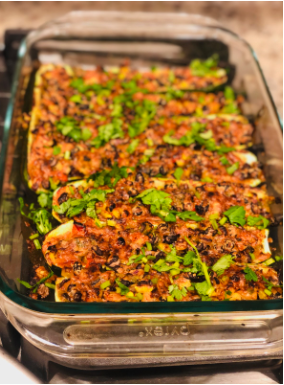
\includegraphics{pictures/zucchini-burrito-boat.png}
\caption{Zucchini Burrito Boat}
\end{figure}

Ready in 45 minutes. Serves 4-5 people.

\hypertarget{ingredients-4}{%
\subsection{Ingredients}\label{ingredients-4}}

\begin{enumerate}
\def\labelenumi{\arabic{enumi}.}
\item
  Zucchini 4
\item
  Kidney beans 14 oz can, drained and rinsed
\item
  Tomato 1 diced
\item
  Coriander 1/4 cup
\item
  Onion diced 1 cup
\item
  Boiled sweet corns 1/2 cup
\item
  Grated cheese Mexican blend 1/2 cup
\item
  Mixed colored peppers 1 cup
\item
  Jalapenos 1 deseeded and finely chopped (optional)
\item
  Salsa spicy
\item
  Salsa medium.
\item
  Lemon juice 1 tbsp
\item
  Salt 1 tsp
\item
  Cumin powder 2 tsp
\item
  Paprika 1 tsp
\item
  Taco seasoning 2 tsp
\item
  Olive oil 2 tbsp
\end{enumerate}

\hypertarget{preparation-4}{%
\subsection{Preparation}\label{preparation-4}}

\begin{enumerate}
\def\labelenumi{\arabic{enumi}.}
\item
  Preheat the oven at 400 °C. Cut zucchini in half lengthwise and scrape out the center part, leaving a shell of almost 1/4 inch thick.
\item
  Sprinkle the taco seasoning generously on them, drizzle olive oil and bake them for 15 minutes.
\item
  In the meantime, in a big bowl add drained and washed kidney beans, tomato, coriander, onions, sweet corn, colored peppers, jalapenos, cumin powder, salt, paprika, half of the cheese and lemon juice. Toss all the ingredients to mix well and get evenly seasoned.
\item
  Take the zucchini shells out of the oven. With a help of a spoon fill the zucchini shells with the above mixture. Sprinkle some cheese on the top.
\item
  Place them again in the oven for 15-20 minutes. Change the setting to broil (High Mode) and broil it for 3 to 5 minutes to get the golden browned top.
\item
  Serve them hot, before serving garnish them with spicy and medium salsa and some finely chopped coriander.
\end{enumerate}

Tip:
Looking for some low carb sides? You can also serve them as appetizers at your holiday get-together. Though this is low carb, it can still take you out of ketosis. Use the leftover scraps of zucchini to make a soup or other dish.

\hypertarget{protein-gelato}{%
\section{Protein Gelato}\label{protein-gelato}}

\begin{figure}
\centering
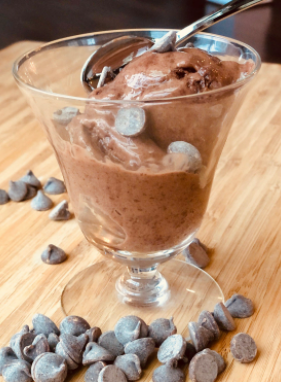
\includegraphics{pictures/protein-gelato.png}
\caption{Protein Gelato}
\end{figure}

Ready in 15 minutes. Serves 5 people. Rest time 3 hours.

\hypertarget{ingredients-5}{%
\subsection{Ingredients}\label{ingredients-5}}

\begin{enumerate}
\def\labelenumi{\arabic{enumi}.}
\item
  2 of Premier Protein Chocolate Shake or any other ready to drink Chocolate shake.
\item
  1 Sugar free Jell-O Chocolate (4 1/2 cups of servings pack)
\item
  Chocolate chips (for garnishing)
\end{enumerate}

\hypertarget{preparation-5}{%
\subsection{Preparation}\label{preparation-5}}

\begin{enumerate}
\def\labelenumi{\arabic{enumi}.}
\item
  In a big bowl empty both the chocolate drinks, add Jell-O and whisk it well for 2 mins. Let it rest for 5 mins and then whisk again.
\item
  Let it stay in the freezer for 1 hour and then take it out and whisk again. Repeat this again after one hour, this time blend it in a blender for creamier texture. You can repeat this one more time for extra creamy texture.
\item
  You can make this in advance and serve it the day of your dinner. When you want to serve, let it stay out of the freezer for 5 mins before serving. For best results, churn it just before serving. Serve it with some chocolate chips sprinkled on the top.
\end{enumerate}

\hypertarget{baked-brussel-sprouts}{%
\section{Baked Brussel Sprouts}\label{baked-brussel-sprouts}}

\begin{figure}
\centering
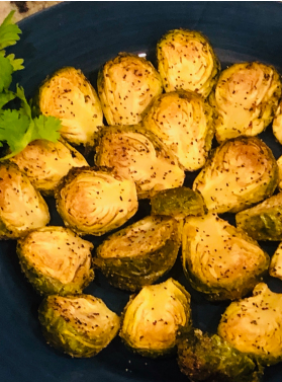
\includegraphics{pictures/baked-brussel-sprouts.png}
\caption{Baked Brussel sprouts}
\end{figure}

Ready in 25 minutes. Serves 2 people.

\hypertarget{ingredients-6}{%
\subsection{Ingredients}\label{ingredients-6}}

\begin{enumerate}
\def\labelenumi{\arabic{enumi}.}
\item
  Brussel Sprouts 4 cups cut in half (Stem side)
\item
  Kosher Salt 1/3 tsp
\item
  Black Pepper 1/4 tsp
\item
  Olive oil 1 tsp
\end{enumerate}

\hypertarget{preparation-6}{%
\subsection{Preparation}\label{preparation-6}}

\begin{enumerate}
\def\labelenumi{\arabic{enumi}.}
\item
  Heat the oven at 400 ° F. In a bowl add the cut Brussel sprouts and sprinkle salt and pepper. Drizzle the oil and toss them well so it gets well coated with the seasoning.
\item
  Place them on a baking tray with all face down (with cut side down) and bake them for 10 minutes.
\item
  Flip them and bake further for 10 minutes.
\item
  Serve them hot with your choice of protein.
\end{enumerate}

\hypertarget{garden-fresh-omelette}{%
\section{Garden Fresh Omelette}\label{garden-fresh-omelette}}

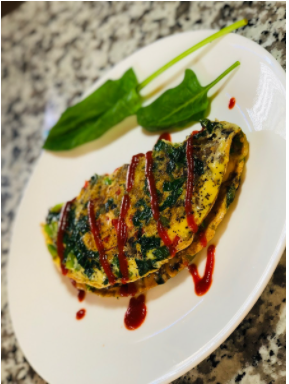
\includegraphics{pictures/garden-fresh-omlette.png}
Ready in 20 minutes. Serves 1.

\hypertarget{ingredients-7}{%
\subsection{Ingredients}\label{ingredients-7}}

\begin{enumerate}
\def\labelenumi{\arabic{enumi}.}
\item
  Eggs 2
\item
  Spinach 1/4 cup
\item
  Peppers (multi-color) 1/4 cup
\item
  Coriander finely chopped 1 tbsp
\item
  Diced Mushroom 1/4 cup
\item
  Salt 1/4 tsp
\item
  Black pepper powder 1/4 tsp
\item
  Feta Cheese 1 1/2 tsp (optional)
\end{enumerate}

\hypertarget{preparation-7}{%
\subsection{Preparation}\label{preparation-7}}

\begin{enumerate}
\def\labelenumi{\arabic{enumi}.}
\item
  Break the eggs in a bowl, add salt pepper powder and beat it well.
\item
  Heat a pan and spray some oil, add all the cut vegetables and stir them for 3 to 4 mins. The spinach will reduce in size.
\item
  Now add the beaten egg on top and cover the pan with a lid.
\item
  Add cheese and flip it in half. Cook it through and serve hot with sriracha sauce.
\end{enumerate}

\hypertarget{from-here-where}{%
\chapter{From here, where?}\label{from-here-where}}

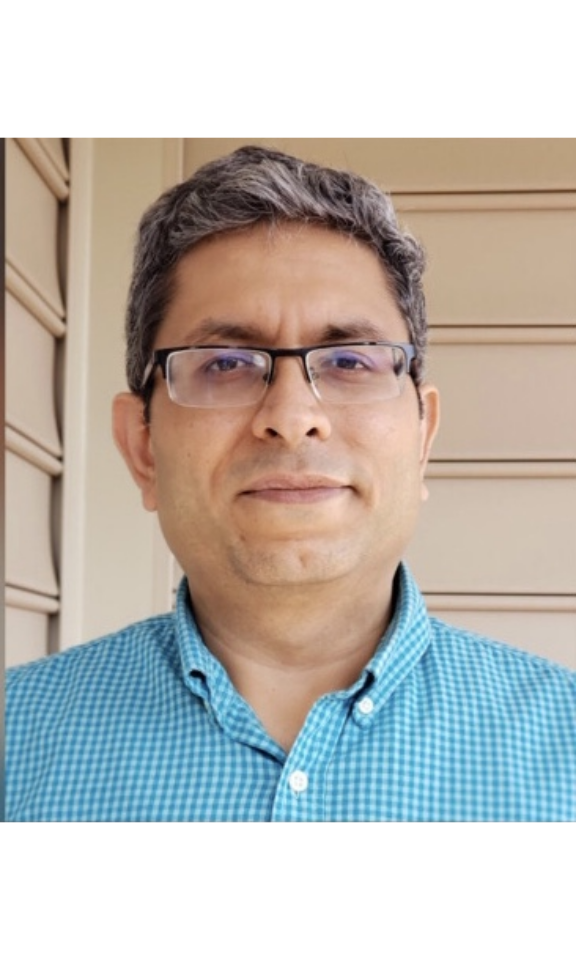
\includegraphics{bookdownproj_files/figure-latex/unnamed-chunk-28-1.pdf}

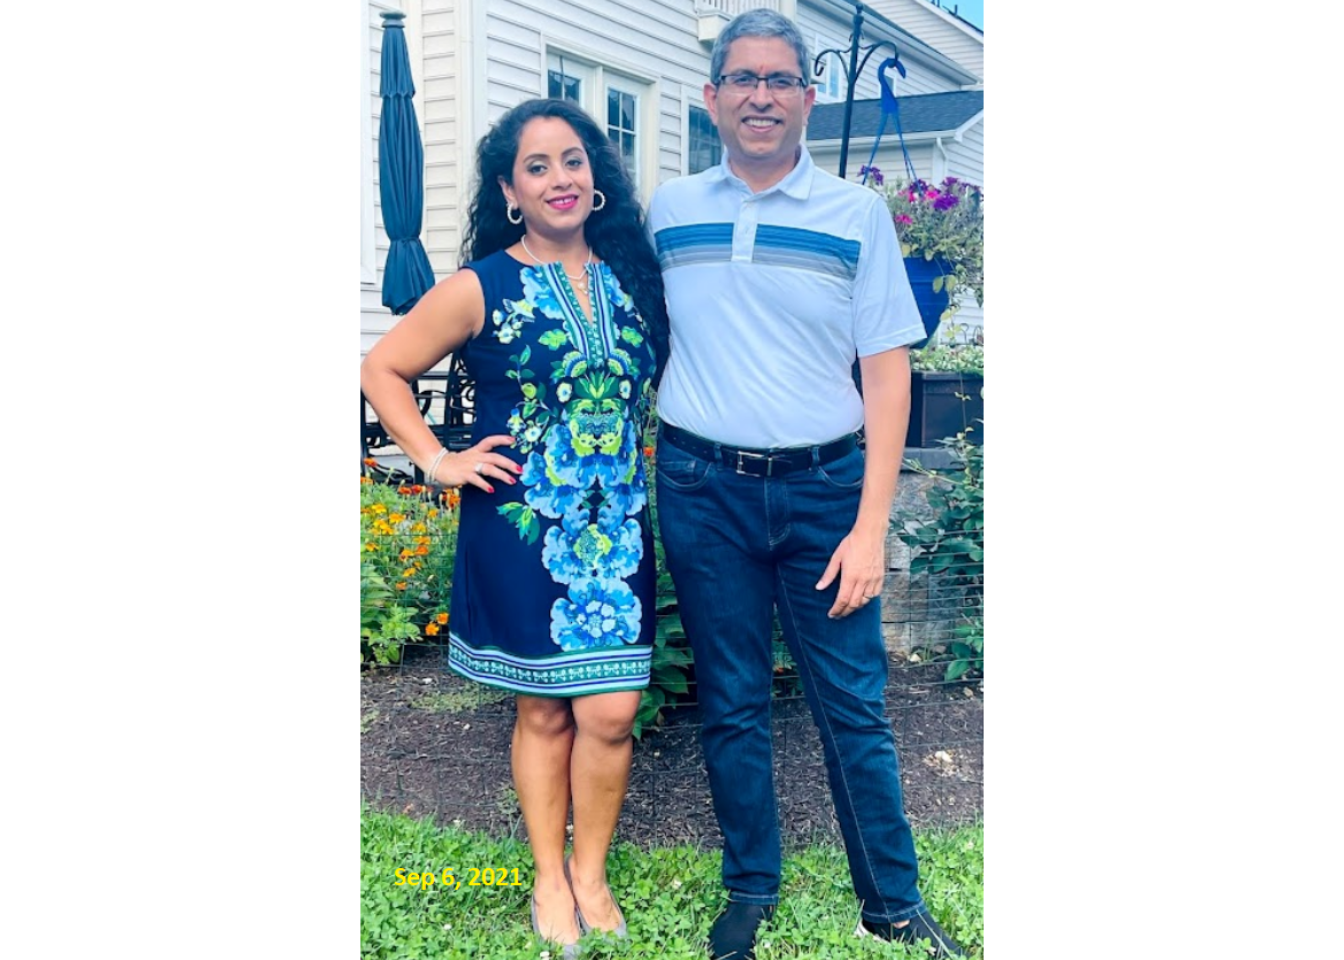
\includegraphics{bookdownproj_files/figure-latex/unnamed-chunk-29-1.pdf}

Here are the customary before, after and the not so customary the year after pictures. I am not a particularly picture friendly person but I do think a picture here highlights the amount of change much more so than numbers ever can.

The good thing about journaling (or writing a book for that matter) is that when you go back and revisit the written word it immediately transports you back in time and then hindsight makes you realize ``oh, that is what I was thinking, how naive was I?''. What I think now about the road ahead is different from what I was thinking same time last year which is documented in the first edition of this book. Last year I was thinking purely in terms of fitness goals but now my field of view is much wider. Anyhow, I am keeping the section from the first edition as is and adding a new one for the second edition as well.

\hypertarget{the-road-ahead-the-2021-version}{%
\section{The road ahead, the 2021 version}\label{the-road-ahead-the-2021-version}}

While 2 years of work cannot bring back 2 lost decades of very little work on my physical and mental health, but the human body is still a very resilient machine. As I write at another place in this book ``the right time to start was yesterday, the best time to start is today!''.

I want to extend my new found levels of physical fitness and ability to focus to explore things I always wanted to do but never thought I could do: be a more outdoors person and spend more time in nature (hiking, mountaineering), learn new skills (swimming), read more books (8 books and counting in 2021), teach at a university, but most importantly, find a purpose that puts everything in perspective and makes everything worthwhile.

I was never good at sports growing up; however I vividly remember one winter afternoon while I was in college and playing cricket, I was hitting everything out of the park. I could not believe that it was me timing the ball to perfection, finding gaps in the field, and hitting fours and sixes. And then just like that, it was gone, I could never repeat what I did that one afternoon, until more than two decades later one morning in the gym when I was doing a circuit of heavy deadlifts. I experienced what people call the \textbf{flow} state, I was able to achieve a 1 rep max on the deadlift and then go on to do the same on the benchpress, my focus was razor sharp, I felt no fatigue, heart rate was normal and I felt I could go on and on (it is especially at such times you need a good trainer who takes an executive decision to say no, this is enough, we are stopping now). It was a magical feeling and unlike that one winter afternoon of decades past, I do not want it to be a moment in time. I want to keep experiencing it now, and decades from now.

\hypertarget{the-road-ahead-from-the-first-edition}{%
\section{The road ahead, from the first edition}\label{the-road-ahead-from-the-first-edition}}

What do we do when our target is met? The proverbial last mile is extremely hard as we are finding out and you can see in the charts presented in the previous chapters. Going with the optimistic assumption that we will achieve our weight and strength targets in the next 2 to 3 months, what do we do next?

The natural answer is that sustaining ourselves at that level of health is going to be a challenge in itself and a tough one at that. What I feel at this time is that this has been such a hard fought (not to mention expensive) battle that the very thought that this could all go away sends a chill down the spine. It is also true that I have been up this hill before and slid back.

What is going to help is to set a new target, that will change the problem from just being one of sustenence to one of achieving a new target. Setting your eyes on the next peak gives an aspirational goal to look up to. Aspirations make you wake up in the morning and get moving. When aspirations are standing on the legs of recent achievements, anything is possible.

My younger one wants to get into wrestling, he is 7 years old. Maybe he and I will train together some day! Let's see where this mid-life ``obsession'' takes me.

\hypertarget{postscript}{%
\section{Postscript}\label{postscript}}

What I realized over the past two years was that what most people perceive as a \textbf{``boring \& disciplined'' life is actually a ``healthy and therefore happy'' life}. I am a person of far less eloquence to say it better than this quote (\href{https://www.univie.ac.at/logotherapy/quote_stimulus.html}{ascribed to Victor Frankel})

Between stimulus and response lies a space. In that space lie our freedom and power to choose a response. In our response lies our growth and our happiness.

\hypertarget{post-postscript}{%
\section{Post Postscript}\label{post-postscript}}

My learning from the past 2 years can be summarized into the following three bullet points:

\begin{itemize}
\item
  Put a high premium on your sleep, do not compromise on sleep for frivolous activities (say no to \href{https://en.wikipedia.org/wiki/Bedtime_procrastination}{bedtime procrastination}). 8 hours of good sleep is probably the single most important thing you can do for your health.
\item
  Reduce processed food (flour, sugar) from your diet, as much as possible and stick to consuming food in an eating window that is consistent both in terms of duration and time of day (mine is 16:8, but 12:12 would usually work for most people).
\item
  Have a consistent strength training regimen, 3 to 5 times a week. You want to do this not just for building a fit body but also (and more importantly) a sharper brain.
\end{itemize}

I sincerely believe that following the above three points would help achieving the worthy goal of long-term health.

\hypertarget{about-the-author}{%
\chapter{About the author}\label{about-the-author}}

\includegraphics{bookdownproj_files/figure-latex/unnamed-chunk-30-1.pdf}

My name is Amit Arora. I live in Clarksburg, Maryland with my wife Nidhi and two sons Nabhit (12) and Aadit (8). I have a bachelor's degree in engineering and a master's degree in data science. I love reading, writing, working with data, and yes, strength training.

If you would like to reach out to me for comments or questions, please feel free to write to me at \url{amiarora@gmail.com}. You can find me on Twitter at \href{https://twitter.com/aarora79}{aarora79}, Instagram \href{https://www.instagram.com/ilivethedata/}{ilivethedata} and at LinkedIn at \url{https://www.linkedin.com/in/amit-arora-539120a/}. Send your tweets and Instagram posts about this book with the hashtag \textbf{\#blueberriesinmysalad}.

\hypertarget{podcasts-videos-and-references}{%
\chapter{Podcasts, Videos and References}\label{podcasts-videos-and-references}}

As one of my professors in graduate school used to say, read this for cultural enrichment, I am providing here a list of links from the Internet that I stumbled upon and found useful. Hope you find these useful as well.

\hypertarget{general}{%
\section{General}\label{general}}

\textbf{The Huberman Lab Podcast}

\url{https://hubermanlab.com/}

This podcast is at the top of my list and for good reason. Imagine being able to sit in a class with a professor patiently delving into the depths of latest research but keeping the material at a level consumable by informed and interested individuals. This is that podcast. Dr Huberman talks about all things health, whether it is sleep, hormones, circadian rhythms, muscle building and so much more. The best part is that he explains the mechanics of why things work the way they work and then provides protocols that can be (relatively) easily incorporated into daily life. I have benefited immensely from this podcast.

\textbf{The Rich Roll Podcast}

\url{https://www.richroll.com/all-episodes/}

I stumbled upon this one following YouTube recommendations and got hooked immediately. Every week, Rich talks to guests about mindset, human performance and of course nutrition and health. Rich's own life story is fascinating, and I would highly recommend reading his very motivational and illuminating autobiography ``Finding Ultra''.

\textbf{Found My Fitness by Dr Rhonda Patrick}

\url{https://www.foundmyfitness.com/}

If you like an academic take on the latest research in health \& fitness, then you will love this.

\hypertarget{supplements}{%
\section{Supplements}\label{supplements}}

\textbf{Dr Rhonda Patrick's supplement list (not endorsed by her)}

\url{https://fastlifehacks.com/dr-rhonda-patricks-supplements-list/}

I found this page by literally doing a Google search one day thinking, I have watched so many of her videos, wonder what supplements does she take?

\hypertarget{circadian-rhythm-tre}{%
\section{Circadian Rhythm \& TRE}\label{circadian-rhythm-tre}}

\textbf{Dr Satchin Panda's TED Talk on Circadian Rhythm}

\url{https://www.youtube.com/watch?v=erBJuxVR7IE}

Health lies in healthy circadian habits.

\textbf{Dr Satchin Panda with Dr Rhonda Patrick on TRE and Circadian Rhythm}

\url{https://www.youtube.com/watch?v=-R-eqJDQ2nU}

90 minutes of extremely detailed discussion on Circadian Rhythm and TRE.

\hypertarget{fasting-mimicking-diet}{%
\section{Fasting Mimicking Diet}\label{fasting-mimicking-diet}}

\textbf{Dr Valter Longo with Dr Rhonda Patrick on fasting mimicking diet and it's effect on longevity and serious diseases}

\url{https://www.youtube.com/watch?v=d6PyyatqJSE}

How fasting helps in ways you may not have thought of.

\hypertarget{exercise}{%
\section{Exercise}\label{exercise}}

\textbf{Jason Walsh, how do actors get ready in shape for movies}

\url{https://www.youtube.com/watch?v=y5-R-TICKSw}

Inspirational!

\textbf{Aamir Khan, Dangal body transformation}

\url{https://www.youtube.com/watch?v=1aVw1gZ9Ncg}

I watch this if I ever feel like skipping a workout!!

\hypertarget{appendix-a}{%
\chapter{Appendix A}\label{appendix-a}}

\hypertarget{food-checklist-for-clean-eating-challenge}{%
\section{Food checklist for clean eating challenge}\label{food-checklist-for-clean-eating-challenge}}

This table lists the food items we could think of (from what we generally eat) in each of the categories listed for the 30-day clean eating challenge. It also contains certain other categories that we added based on the food items in our pantry. The purpose here was to get a clear Yay or Nay listed alongside each food item so that we knew exactly what is allowed and did not end up with a day 0 crisis at our hands.

\begin{longtable}[t]{lll}
\toprule
Food Category & Food Item & Allowed?\\
\midrule
\endfirsthead
\multicolumn{3}{@{}l}{\textit{(continued)}}\\
\toprule
Food Category & Food Item & Allowed?\\
\midrule
\endhead

\endfoot
\bottomrule
\endlastfoot
Meat \& Fish & Lamb & Y\\
Meat \& Fish & Goat & Y\\
Meat \& Fish & Chicken & Y\\
Meat \& Fish & Salmon & Y\\
Meat \& Fish & Tilapia & N
Prefer Cod\\
\addlinespace
Meat \& Fish & Shrimp & Y\\
Meat \& Fish & Ham & Y\\
Eggs & Organic Cage Free & Y\\
Vegetables & Turnip & Y\\
Vegetables & Spinach & Y\\
\addlinespace
Vegetables & Kale & Y\\
Vegetables & Dill & Y\\
Vegetables & Fenugreek & Y\\
Vegetables & Lettuce & Y\\
Vegetables & Curry Leaves & Y\\
\addlinespace
Vegetables & Mustard Leaves & Y\\
Vegetables & Carrots & Y\\
Vegetables & Radish & Y\\
Vegetables & Zucchini & Y\\
Vegetables & Squash & Y\\
\addlinespace
Vegetables & Brussel Sprouts & Y\\
Vegetables & Broccoli & Y\\
Vegetables & Peppers & Y\\
Vegetables & Snow Peas & Y\\
Vegetables & Peas & Y\\
\addlinespace
Vegetables & Celery & Y\\
Vegetables & Tomato & Y\\
Vegetables & Brinjal & Y\\
Vegetables & Spring Onions & Y\\
Vegetables & Beet Roots & Y\\
\addlinespace
Vegetables & Avocado & Y\\
Vegetables & Okra & Y\\
Vegetables & Cauliflower & Y\\
Vegetables & Sweet Potato & Y\\
Vegetables & Tindora & Y\\
\addlinespace
Vegetables & Bitter Gourd & Y\\
Vegetables & Bottle Gourd & Y\\
Vegetables & Cucumber & Y\\
Vegetables & Green Papaya & Y\\
Nuts & Almond & Y
Keep to a minimum\\
\addlinespace
Nuts & Pistachio & Y\\
Nuts & Walnut & Y\\
Nuts & Peanuts & Y\\
Dried Fruits & Raisins & Y
Upto 2oz/day of dried fruits\\
Dried Fruits & Cranberry & Y\\
\addlinespace
Dried Fruits & Dates (please approve!) & Y\\
Dried Fruits & Apricots & Y\\
Dried Fruits & Prunes & Y\\
Dried Fruits & Figs & Y\\
Seeds & Sunflower & Y\\
\addlinespace
Seeds & Melon & Y\\
Seeds & Chia & Y\\
Seeds & Basil & Y\\
Seeds & Mustard & Y\\
Seeds & Fenugreek & Y\\
\addlinespace
Seeds & Sesame & Y\\
Seeds & Fennel & Y\\
Fruits & Blueberry & Y
Upto 3servings/week of fruits\\
Fruits & Strawberry & Y\\
Fruits & Blackberry & Y\\
\addlinespace
Fruits & Raspberry & Y\\
Fruits & Kiwi & Y\\
Fruits & Pomegranate & Y\\
Fruits & Pears & Y\\
Fruits & Papaya & Y\\
\addlinespace
Fruits & Pineapple & Y\\
Fruits & Orange & Y\\
Fruits & Cantaloupe & Y\\
Fruits & Watermelon & Y\\
Fruits & Peach & Y\\
\addlinespace
Fruits & Plum & Y\\
Fruits & Apple (green and red) & Y\\
Fruits & Banana & Y\\
Fruits & Grapes & Y\\
Fruits & Star fruit & Y\\
\addlinespace
Fruits & Guava & Y\\
Fruits & Honey dew & Y\\
Fruits & Mango & Y\\
Oils & Olive oil & Y\\
Oils & Ghee & Y\\
\addlinespace
Oils & Avocado Oil & Y\\
Oil & Canola Oil & Y\\
Oil & Seasme seed oil & Y\\
Oil & Kerrygold butter & Y\\
Herbs \& Spices & Lemon & Y\\
\addlinespace
Herbs \& Spices & Curry Leaves & Y\\
Herbs \& Spices & Parsley & Y\\
Herbs \& Spices & Coriander & Y\\
Herbs \& Spices & Turmeric & Y\\
Herbs \& Spices & Salt & Y\\
\addlinespace
Herbs \& Spices & Cajun Spice & Y\\
Herbs \& Spices & Asafetida & Y\\
Herbs \& Spices & Cardamom & Y\\
Herbs \& Spices & Black Cardamom & Y\\
Herbs \& Spices & Red Chillies & Y\\
\addlinespace
Herbs \& Spices & Oregano & Y\\
Herbs \& Spices & Lemon Leaves & Y\\
Herbs \& Spices & Cloves & Y\\
Herbs \& Spices & Cinnamon & Y\\
Herbs \& Spices & Pepper & Y\\
\addlinespace
Herbs \& Spices & Whole Black Pepper & Y\\
Herbs \& Spices & Garlic & Y\\
Herbs \& Spices & Ginger & Y\\
Herbs \& Spices & Saffron & Y\\
Herbs \& Spices & Cloves & Y\\
\addlinespace
Milk & Dairy & N\\
Milk & Almond milk & Y\\
Milk & Coconut Milk & Y\\
Others & Soy Sauce & Y
Gluten free only\\
Others & Schezwan Sauce & Y\\
\addlinespace
Others & Chilly Garlic Paste & Y\\
Others & Sparkling Water & Y\\
Others & Selzer Water & Y\\
Others & Club Soda & N\\
Others & Black Coffee & Y\\
\addlinespace
Others & Tea & Y\\
Others & Caffeine free tea & Y\\
Others & Aloe Vera & Y\\
Others & Honey & Y
Very sparingly\\
Others & Off the shelf dressings & N\\
\addlinespace
Others & Mustard Sauce & Y\\
Others & Vinegar & Y\\*
\end{longtable}

\end{document}
